\documentclass[12pt, titlepage, french]{report}
%% -----------------------------
%% Encodage
%% -----------------------------
\usepackage[utf8]{inputenc}
\usepackage[T1]{fontenc}
\usepackage{babel}
\usepackage{lmodern}
%
%%% -----------------------------
%%% Définition de variables
%%% -----------------------------
%\def\auteur{Alec James van Rassel}
%\def\BackgroundColor{white}
%
%%% -----------------------------
%%% Margin and layout
%%% -----------------------------
%% Determine the margin for cheatsheet
%\usepackage[landscape, hmargin=1cm, vmargin=1.7cm]{geometry}
\usepackage{multicol}
\usepackage{sectsty}
\usepackage{titlesec}
%%% -----------------------------
%%%	Sections et chapitres
%%% -----------------------------
\titleformat{\chapter}
  {\normalfont\LARGE\bfseries}{\thechapter}{1em}{}
\titlespacing*{\chapter}{0pt}{3.5ex plus 1ex minus .2ex}{2.3ex plus .2ex}
\sectionfont{\color{cobalt}}
\subsectionfont{\color{indigo(web)}}
%%%
%%%	Avec cette commande, \section à le même comportement que \section* mais les sections apparaissent dans le TOC;
%%%	-	Ceci est appliqué aux sous-sections et sous-sous-sections, pas uniquement aux sections.
%
\setcounter{secnumdepth}{0}
%%%
%%%	Pour inclure les sous-sections dans la table des matières (TOC).
%%%
%%	Niveaux pour les classes book et report:
%%	-1:	part;			0:	chapter;		1:	section;			2:	subsection;	
%%	3:	subsubsection;	4:	paragraph;	5:	subparagraph;
%%	NOTE:	0 existe seulement pour les classes book et report et est part pour la class article.
%%%
\setcounter{tocdepth}{3}

%% -----------------------------
%% URL and links
%% -----------------------------
\usepackage{hyperref}
\usepackage{nameref}
\hypersetup{colorlinks = true, urlcolor = white, linkcolor = black}

%% -----------------------------
%% Document policy (en décommenter seulement une)
%% -----------------------------
%	\usepackage{concrete}
%	\usepackage{mathpazo}
%	\usepackage{frcursive} %% permet d'écrire en lettres attachées
%	\usepackage{aeguill}
%	\usepackage{mathptmx}
%	\usepackage{fourier} 

%% -----------------------------
%% Math configuration
%% -----------------------------
\usepackage[fleqn]{amsmath}
\usepackage{amsthm, amssymb, latexsym, amsfonts}
\usepackage{empheq}
\usepackage{numprint}
\usepackage{dsfont} % Pour avoir le symbole du domaine Z

%%% -----------------------------
%%% Raccourcis mathématiques
%%% -----------------------------
\newcommand{\reels}{\mathbb{R}}
\newcommand{\entiers}{\mathbb{Z}}
\newcommand{\naturels}{\mathbb{N}}
\newcommand{\eval}{\biggr \rvert}
\usepackage{cancel}
\newcommand{\derivee}[1]{\frac{\partial}{\partial #1}}
\newcommand{\prob}[1]{\Pr \left( #1 \right)}
\newcommand{\esp}[1]{\mathrm{E} \left[ #1 \right]} % espérance
\newcommand{\variance}[1]{\mathrm{Var} \left( #1   \right)}
\newcommand{\covar}[1]{\mathrm{Cov} \left( #1   \right)}
\newcommand{\laplace}{\mathcal{L}}
\newcommand{\deriv}[2][]{\frac{\partial^{#1}}{\partial #2^{#1}}}
\newcommand{\e}[1]{\mathrm{e}^{#1}}
\newcommand{\te}[1]{\text{exp}\left\{#1\right\}}
\DeclareMathSymbol{\shortminus}{\mathbin}{AMSa}{"39}

% To indicate equation number on a specific line in align environment
\newcommand\numberthis{\addtocounter{equation}{1}\tag{\theequation}}


%%% -----------------------------
%%% 	Paquetage de notation actuarielle
%%% -----------------------------
\usepackage{actuarialsymbol}
\usepackage{actuarialangle}

%%% -----------------------------
%%% Notation matricielle pour les symboles mathématiques
%%%
%%  (\bm{•})
%%% -----------------------------
\usepackage{bm}
%% Notation matricielle pour les variables
\newcommand{\matr}[1]{\mathbf{#1}}

%% -----------------------------
%% Configuration de tcolorbox
%% -----------------------------
\usepackage[most]{tcolorbox}
\tcbuselibrary{xparse}
\tcbuselibrary{breakable}
%%	-----------------------------
%%
%%	Arguments du paquetage
%%	+	breakable: allows box to be split over several pages
%%	+	segmentation style: To customize the \tcbline seperator
%%	
%%	-----------------------------
%%

%%
%% Coloured box "definition" for definitions
%%
\DeclareTColorBox{theorems}{ o}			% #1 parameter
{
	enhanced,
	title = #1,
	colback=bluebell, % color of the box
	colframe=blue(pigment),
	colbacktitle=blue!80!black,
	fonttitle = \bfseries,
	boxed title style={size=small,colframe=purple!50!black} ,
	attach boxed title to top center = {yshift=-3mm,yshifttext=-1mm},
	left=0pt,
  	right=0pt,
    box align=center,
    ams align*
%  	top=-10pt
}
\DeclareTColorBox{distributions}{ o }			% #1 parameter
{
	enhanced,
	title = #1,
	colback=ashgrey, % color of the box
%	colframe=blue(pigment),
	breakable,
	colframe=arsenic,	
	colbacktitle=aurometalsaurus,
	fonttitle = \bfseries,
	boxed title style={size=small,colframe=arsenic} ,
	attach boxed title to top center = {yshift=-3mm,yshifttext=-1mm},
%	left=0pt,
%  	right=0pt,
%    box align=center,
%    ams align*
%  	top=-10pt
}
\DeclareTColorBox{outcomes}{ o }			% #1 parameter
{
	enhanced,
	title = #1,
	colback=bluebell, % color of the box
%	colframe=blue(pigment),
%	colframe=asparagus,	
	breakable,
	colbacktitle=airforceblue,
	fonttitle = \bfseries,
	boxed title style={size=small,colframe=arsenic} ,
	attach boxed title to top center = {yshift=-3mm,yshifttext=-1mm},
%	left=0pt,
%  	right=0pt,
%    box align=center,
%    ams align*
%  	top=-10pt
}
\DeclareTColorBox{ASM_chapter}{ o }			% #1 parameter
{
	enhanced,
	title = #1,
	colback=darkseagreen, % color of the box
%	colframe=blue(pigment),
%	colframe=asparagus,	
	colbacktitle=britishracinggreen,
	fonttitle = \bfseries,
	boxed title style={size=small,colframe=arsenic} ,
	attach boxed title to top center = {yshift=-3mm,yshifttext=-1mm},
	segmentation style = {dashed, white},
	breakable
%	left=0pt,
%  	right=0pt,
%    box align=center,
%    ams align*
%  	top=-10pt
}
\DeclareTColorBox{YTB_vids}{ o }			% #1 parameter
{
	enhanced,
	title = #1,
	colback=red_rectangle, % color of the box
%	colframe=blue(pigment),
%	colframe=asparagus,	
	colbacktitle=lava,
	fonttitle = \bfseries,
	boxed title style={size=small,colframe=arsenic} ,
	attach boxed title to top center = {yshift=-3mm,yshifttext=-1mm},
	segmentation style = {dashed, white},
	breakable
%	left=0pt,
%  	right=0pt,
%    box align=center,
%    ams align*
%  	top=-10pt
}
%%
%% Coloured box "algo" for algorithms
%%
\newtcolorbox{algo}[ 1 ]
{
	colback = blue!5!white,
	colframe = blue!75!black,
	fonttitle = \bfseries,title=#1
}
%%
%% Coloured box "formula" for formulas
%%
\newtcolorbox{formula}[ 1 ]
{
	colback = green!5!white,
	colframe = darkseagreen,
	fonttitle = \bfseries,title=#1
}
%%
%% Coloured box "CHPT_SUMM" pour résumés des chapitres de l'ASM
%%
%\newtcolorbox[auto counter]{CHPT_SUMM}[ 2 ][] 	%pour ajouter du numérotage automatique
\newtcolorbox{CHPT_SUMM}[ 2 ][]
{
	colback = green!5!white,
	colframe = darkseagreen,
	breakable,
	enhanced,
	fonttitle = \bfseries,
%	title = Chapitre~\thetcbcounter: #2, 		pour inclure le numérotage automatique
	title = #2,
	#1
}
\newtcolorbox[list inside = CHPT]{CHPT_SUMM_AUTO}[ 2 ][]
{
	colback = green!5!white,
	colframe = darkseagreen,
	breakable,
	enhanced,
	fonttitle = \bfseries,
%	title = Chapitre~\thetcbcounter: #2, 		pour inclure le numérotage automatique
	title = #2,
	nameref = #2,
	after upper = {\addcontentsline{toc}{subsubsection}{#2}},
%	phantomlabel = {#2},
	#1
}
\newtcolorbox[auto counter, list inside = CHPT]{CHPT_SUMM_AUTO_NUMB}[ 2 ][]
{
	colback = green!5!white,
	colframe = darkseagreen,
	breakable,
	enhanced,
	fonttitle = \bfseries,
	title = Chapter~\thetcbcounter: #2, 		
%	title = #2,
	nameref = #2,
	after upper = {\addcontentsline{toc}{subsubsection}{\thetcbcounter: #2}},
%	phantomlabel = {#2},
	#1
}
%%
%% Coloured box "FORMULA_SUMM" pour résumés des formules de l'ASM
%%
\newtcolorbox{FORMULA_SUMM}[ 1 ]
{
	colback = babyblueeyes,
	colframe = airforceblue,
	breakable,
	fonttitle = \bfseries,title=#1
}
%%
%% Coloured box "YTB_SUMM" pour résumés des vidéos Youtube
%%
\newtcolorbox{YTB_SUMM}[ 2 ][]
{
	colback = red!5!white,
	colframe = darkterracotta,
	breakable,
	enhanced,
%	    frame hidden,
	fonttitle = \bfseries,
	title=#2,
	#1
}

%% -----------------------------
%% Graphiques et images
%% -----------------------------
\usepackage{graphicx}
\usepackage{pict2e}
\usepackage{tikz}

%%
%%	Crée un cercle
%%	Arguments:
%%	+	size
%%	+	colour
%%	
%%	Example:
%%	+	\tikzcircle[green, fill=blue]{1.5pt}
%%	+	\tikzcircle{2pt}
%%
\newcommand{\tikzcircle}[2][red,fill=red]{\tikz[baseline=-0.5ex]\draw[#1,radius=#2] (0,0) circle ;}

%%% -----------------------------
%%% insérer des pages pdf dans un document
%%% -----------------------------
\usepackage{pdfpages}

%%% -----------------------------
%%% Color configuration
%%% -----------------------------
\usepackage{color, soulutf8, colortbl}

%%% -----------------------------
%%%	Définitions de couleurs
%%% -----------------------------
\definecolor{darkterracotta}{rgb}{0.8, 0.31, 0.36}   % red pastel ish
\definecolor{lava}{rgb}{0.81, 0.06, 0.13}
\definecolor{wildwatermelon}{rgb}{0.99, 0.42, 0.52}  % red ish
\definecolor{bostonuniversityred}{rgb}{0.8, 0.0, 0.0} % rich red
\definecolor{asparagus}{rgb}{0.53, 0.66, 0.42}		% sorta militarygreen but pastel
\definecolor{darkseagreen}{rgb}{0.56, 0.74, 0.56}    % pastel light green
\definecolor{britishracinggreen}{rgb}{0.0, 0.26, 0.15} %dark green
\definecolor{airforceblue}{rgb}{0.36, 0.54, 0.66}	% nice teal blue pastel
\definecolor{babyblueeyes}{rgb}{0.63, 0.79, 0.95}	% pastel blue-ish
\definecolor{applegreen}{rgb}{0.55, 0.71, 0.0}		% green with some aqua
\definecolor{indigo(web)}{rgb}{0.29, 0.0, 0.51}
\definecolor{cobalt}{rgb}{0.0, 0.28, 0.67}
\definecolor{azure(colorwheel)}{rgb}{0.0, 0.5, 1.0}
\definecolor{darkpastelpurple}{rgb}{0.59, 0.44, 0.84}
\definecolor{darkgreen}{rgb}{0.0, 0.2, 0.13}			
\definecolor{burntorange}{rgb}{0.8, 0.33, 0.0}		
\definecolor{burntsienna}{rgb}{0.91, 0.45, 0.32}		
\definecolor{ao(english)}{rgb}{0.0, 0.5, 0.0}		% ACT-2003
\definecolor{amber(sae/ece)}{rgb}{1.0, 0.49, 0.0} 	% ACT-2004
\definecolor{green_rectangle}{RGB}{131, 176, 84}		% ACT-2004
\definecolor{red_rectangle}{RGB}{241,112,113}		% ACT-2004
\definecolor{blue_rectangle}{RGB}{83, 84, 244}		% ACT-2004
\definecolor{blue(pigment)}{rgb}{0.2, 0.2, 0.6}
\definecolor{bluebell}{rgb}{0.64, 0.64, 0.82}
\definecolor{amethyst}{rgb}{0.6, 0.4, 0.8}
\definecolor{amethyst-light}{rgb}{0.6, 0.4, 0.8}
\definecolor{aurometalsaurus}{rgb}{0.43, 0.5, 0.5}
\definecolor{arsenic}{rgb}{0.23, 0.27, 0.29}			%	dark black-grey ish pastel
\definecolor{ashgrey}{rgb}{0.7, 0.75, 0.71}
%
% Useful shortcuts for coloured text
%
\newcommand{\orange}{\textcolor{orange}}
\newcommand{\red}{\textcolor{red}}
\newcommand{\cyan}{\textcolor{cyan}}
\newcommand{\blue}{\textcolor{blue}}
\newcommand{\green}{\textcolor{green}}
\newcommand{\purple}{\textcolor{magenta}}
\newcommand{\yellow}{\textcolor{yellow}}

%% -----------------------------
%% Enumerate environment configuration
%% -----------------------------
%
% Custum enumerate & itemize Package
%
\usepackage{enumitem}
%
% French Setup for itemize function
%
\frenchbsetup{StandardItemLabels=true}
%
% Change default label for itemize
%
\renewcommand{\labelitemi}{\faAngleRight}


%% -----------------------------
%% Tabular column type configuration
%% -----------------------------
\newcolumntype{C}{>{$}c<{$}} % math-mode version of "l" column type
\newcolumntype{L}{>{$}l<{$}} % math-mode version of "l" column type
\newcolumntype{R}{>{$}r<{$}} % math-mode version of "l" column type
\newcolumntype{f}{>{\columncolor{green!20!white}}p{1cm}}
\newcolumntype{g}{>{\columncolor{green!40!white}}m{1.2cm}}
\newcolumntype{a}{>{\columncolor{red!20!white}$}p{2cm}<{$}}	% ACT-2005
% configuration to force a line break within a single cell
\usepackage{makecell}


%% -----------------------------
%% Fontawesome for special symbols
%% -----------------------------
\usepackage{fontawesome}

%
%%% -----------------------------
%%% Footer/Header Customization
%%% -----------------------------
%\usepackage{lastpage}
%\usepackage{fancyhdr}
%\pagestyle{fancy}
%%
%% Page background color
%%
%\pagecolor{\BackgroundColor}


%% END OF PREAMBLE
% ---------------------------------------------
% ---------------------------------------------
%% -----------------------------
%% Section Font customization
%% -----------------------------
\title{
	Guide d'étude	\\
	\large Examen SRM: Statistics for Risk Modeling 	\\
	Society of Actuaries (SOA)}
\vspace{-8ex}
\date{}
\author{Alec James van Rassel}

\begin{document}

\maketitle

\tableofcontents

\clearpage

\part*{Préliminaires}

\section{Rappel des bases de statistiques}

\begin{YTB_vids}[Vidéos YouTube]
\begin{itemize}
	\item	\href{https://www.youtube.com/watch?v=bsZGt-caXO4}{StatQuest: One or Two Tailed P-Values}
	\item	\href{https://www.youtube.com/watch?v=KS6KEWaoOOE}{Khan Academy: P-values and significance tests}
\end{itemize}
\end{YTB_vids}

\subsection{Notes sur les vidéos YouTube}

\begin{YTB_SUMM}{\href{https://www.youtube.com/watch?v=bsZGt-caXO4}{StatQuest: One or Two Tailed P-Values}}
\begin{itemize}
	\item	\textbf{Test} new treatment \tikzcircle[burntorange, fill=burntorange]{3pt} vs old treatment \tikzcircle[black, fill=black]{3pt}
	\begin{itemize}
		\item	One-tailed: $\mathcal{H}_{1}:$ The new treatment \tikzcircle[burntorange, fill=burntorange]{3pt} is \textit{better} than the old treatment \tikzcircle[black, fill=black]{3pt}.
		\item	Two-tailed: $\mathcal{H}_{1}:$ The new treatment \tikzcircle[burntorange, fill=burntorange]{3pt} is \textit{better}, \textit{worse} or \textit{not significantly different} than the old treatment \tikzcircle[black, fill=black]{3pt}.
	\end{itemize}
	\item	\textbf{P-Hacking}
	\begin{itemize}
		\item	Deciding to test if the new treatment \tikzcircle[burntorange, fill=burntorange]{3pt} is \textit{better} rather than \textit{better}, \textit{worse} or \textit{not significantly different} than the old treatment \tikzcircle[black, fill=black]{3pt} \textit{after} seeing the skewed distribution.
	\end{itemize}
	\item	\textbf{False Positive} \textit{(recall the image of the normal distribution with the points)}
	\begin{itemize}
		\item	Usually, the two samples for \tikzcircle[burntorange, fill=burntorange]{3pt} and \tikzcircle[black, fill=black]{3pt} overlap (recall image where they're overlapping) but it can happen that they don't (recall image where they're spaced out) in which case the p-value is less than $0.05$ and we have a \textbf{\textit{false positive}}.
	\end{itemize}
	\item	To decide which $t$ test to use, ask ourselves \textbf{what we want to learn from the test} and then decide.
\end{itemize}
\end{YTB_SUMM}

\begin{YTB_SUMM}{\href{https://www.youtube.com/watch?v=KS6KEWaoOOE}{Khan Academy: P-values and significance tests}}
\begin{itemize}
	\item	Test de signification
	\begin{enumerate}[label=\roman*]
		\item	Déterminer la question
		\item	Établir les connus
	\end{enumerate}
	\begin{enumerate}
		\item	Définir les hypothèses $\mathcal{H}_{0}$ et $\mathcal{H}_{a}$
		\item	Établir un niveau de signification $\alpha$ (souvent $0.05$)
		\item	Obtenir un échantillon
		\item	Trouver la p-value
		\begin{itemize}
			\item	p-value = Pr\{ statistique de test si $\mathcal{H}_{0}$ est vrai \} $\neq$  Pr\{ $\mathcal{H}_{0}$ est vrai sachant la statistique de test \}
		\end{itemize}
		\item	Décider
		\begin{itemize}
			\item	Si p-value $< \alpha$  alors on rejète l'hypothèse nulle
			\item	Si p-value $\geq \alpha$ alors on ne peut pas rejeter l'hypothèse nulle
		\end{itemize}
	\end{enumerate}
\end{itemize}
\end{YTB_SUMM}

\clearpage

\section{Autres ressources}
\begin{FORMULA_SUMM}{Liens}
\begin{itemize}
	\item	\href{https://physics.info/music/}{Article} sur la musique et le bruit;
	\item	\href{https://www.quantstart.com/articles/White-Noise-and-Random-Walks-in-Time-Series-Analysis/}{Article} sur l'analyse de séries chronologiques avec \textsc{R};
\end{itemize}
\end{FORMULA_SUMM}

\part*{Sujets à l'étude}

\chapter[Basics of statistical learning]{Basics of statistical learning (7.5\% à 12.5\%)}

\subsection{Information}

\begin{distributions}[Objective]
Understand key concepts of statistical learning
\end{distributions}

\begin{outcomes}[Learning outcomes]
\begin{enumerate}
	\item	Expliquer les différents types de problèmes, et différentes méthodes, de modélisation. Y compris: 
	\begin{itemize}
		\item	Apprentissage supervisé vs non-supervisé
		\item	Régression vs classification	
	\end{itemize}
	\item	Expliquer les méthodes courantes pour évaluer la précision d'un modèle.
	\item	Utiliser les méthodes de base d'analyse exploratoire de données y compris la validation et vérification de données.
\end{enumerate}
\end{outcomes}

\begin{ASM_chapter}[Related lessons ASM]
\begin{enumerate}
	\item	\hyperref[BASICS]{Basics of Statistical Learning}
\end{enumerate}
\end{ASM_chapter}

\begin{YTB_vids}[Vidéos YouTube]
\begin{itemize}
	\item	\hyperref[SQ-BASICS-ML-INTRO]{StatQuest: A Gentle Introduction to Machine Learning}
	\item	\hyperref[SQ-BASICS-ML-BIASVARIANCE]{StatQuest: Machine Learning Fundamentals: Bias and Variance}
	\item	\hyperref[SQ-BASICS-QUANTILES]{StatQuest: StatQuest: Quantiles and Percentiles, Clearly Explained!!!}
	\item	\hyperref[SQ-BASICS-QQPLOTS]{StatQuest: Quantile-Quantile plots (QQ plots), clearly explained}
	\item	\hyperref[SQ-BASICS-QUANTILE-NORMALISATION]{StatQuest: Quantile Normalization}
\end{itemize}
\end{YTB_vids}

\subsection{Résumés des chapitres}

\begin{CHPT_SUMM}[label = {BASICS}]{\addcontentsline{toc}{subsubsection}{1. Basics of Statistical Learning}1. Basics of Statistical Learning}
	\begin{itemize}
		\item	Définitions de base
		\item	Comparaisons
		\begin{itemize}
			\item	Prévision vs inférence
			\item	Paramétrique vs non-paramétrique 
			\item	Flexibilité vs interprétabilité
			\item	Apprentissage supervisé vs non-supervisé
			\item	Régression vs classification
			\item	Biais vs variance 
		\end{itemize}
		\item	Types de variables
		\begin{itemize}
			\item	Continue
			\item	Catégorique
			\begin{itemize}
				\item[]	S'il y a une ordre logique, c'est \textit{ordinal} sinon nominal.
			\end{itemize}
			\item	Comptage
		\end{itemize}
		\item	Graphiques (scatter, box, qq)
	\end{itemize}
\end{CHPT_SUMM}

\subsection{Notes sur les vidéos YouTube}

\begin{YTB_SUMM}[label = {SQ-BASICS-ML-INTRO}]{\href{https://www.youtube.com/watch?v=Gv9_4yMHFhI&list=PLblh5JKOoLUICTaGLRoHQDuF_7q2GfuJF&index=2&t=0s}{StatQuest: A Gentle Introduction to Machine Learning}}
\begin{itemize}
	\item	Le but de l'apprentissage machine est de faire des \textbf{prévisions}. 
	\item	Les \textit{arbres de décisions} peuvent être utilisés pour la prévision ou la \textbf{classification} et la régression pour la prévision.
	\item	Peut importe la méthode, l'important est de mesurer la \textit{\textbf{précision} des prévisions}.
	\item	On peut donc tester notre méthode avec du \textbf{testing data}.
	\item	\textbf{Bias-Variance tradeoff}: Être bien ajusté, mais avoir des mauvaise prévisions.
\end{itemize}
\end{YTB_SUMM}

\begin{YTB_SUMM}[label = {SQ-BASICS-ML-BIASVARIANCE}]{\href{https://www.youtube.com/watch?v=EuBBz3bI-aA&list=PLblh5JKOoLUICTaGLRoHQDuF_7q2GfuJF&index=6}{StatQuest: Machine Learning Fundamentals: Bias and Variance}}
\begin{itemize}
	\item	\textbf{Biais}: Inhabilité pour une méthode de prévision de capturer la vraie relation. Pour exemple:
	\begin{itemize}
		\item	Essayer de fit une droite aux points du vidéo; évidemment elle ne peut pas reproduire la vraie relation \textbf{VS} une squiggly line qui peut avec little to no biais.
		\item	Alors, la squiggly line sera mieux ajusté aux données d'entrainement mais pas aux testing data; alias, elle sera \textbf{overfitted}.
	\end{itemize}
	\item	\textbf{Variance}: Variance de l'ajustement entre ensembles de données.
	\begin{itemize}
		\item	La squiggly line aura une variance très élevée mais pas la droite; la droite est cohérente et aura toujours un \textbf{SSE} similaire.
	\end{itemize}
	\item	On cherche donc la meilleur combinaison des deux méthodes. Plusieurs méthodes existent pour la trouver dont la \textbf{régularisation}, le \textit{boosting} et le \textit{bagging}.
\end{itemize}
\end{YTB_SUMM}

\begin{YTB_SUMM}[label = {SQ-BASICS-QUANTILES}]{\href{https://www.youtube.com/watch?v=IFKQLDmRK0Y&feature=youtu.be}{StatQuest: StatQuest: Quantiles and Percentiles, Clearly Explained!!!}}
Visualise the chart with the 15 points to which we add the lines.
\begin{enumerate}
	\item	The \textbf{median} is a quantile because it splits the data into 2 equally sized groups.
	\begin{itemize}
		\item	The (0.5 | 50\%) quantile value is 4.5.
	\end{itemize}
	\item	The (0.25 | 25\%) quantile is such that (25\% | a quarter) of the points are less than it.
	\item	\textbf{Technically}, quantiles are line which divide the data into equally sized groups.
	\item	\textbf{Technically}, percentiles are just quantiles which divide the data into 100 equally sized groups.
	\begin{itemize}
		\item	In practice, terminology is much more flexible;
		\item	Even if there's less than 100\%, we still call the ( median | 50\% quantile) the 50$^{th}$ percentile.
		\item	To calculate a quantile / percentile, just calculate how many values are less than it.
	\end{itemize}
	\item	There are many other ways to calculate quantiles, R has 9 just by itself!
	\item	The lesson however, is that the smaller the sample the more variable the results.
\end{enumerate}
\end{YTB_SUMM}

\begin{YTB_SUMM}[label = {SQ-BASICS-QQPLOTS}]{\href{https://www.youtube.com/watch?v=okjYjClSjOg&list=PLblh5JKOoLUIcdlgu78MnlATeyx4cEVeR&index=20}{StatQuest: Quantile-Quantile plots (QQ plots), clearly explained}}
\begin{enumerate}
	\item	Give each data point it's quantile.
	\item	Get a normal curve.
	\item	Add all the quantiles obtained to the curve.
	\begin{itemize}
		\item	That's to say the percentage and not the value.
	\end{itemize}
	\item	Plot QQ graph.
	\begin{itemize}
		\item	If the data were normal, most data points would be on the line;
		\item	If the fit is not good, can try a different distribution;
		\item	Thus, can use the QQ plot to see which distribution fits the data.
	\end{itemize}
\end{enumerate}
\begin{itemize}
	\item	Could also use the QQ plot to compare 2 datasets.
	\item	For example, if the second one had less data points we could use quartiles instead!
	\item	We add the points at the intersection of the 2 datasets' quantiles and add a straight line.
\end{itemize}
\end{YTB_SUMM}

\begin{YTB_SUMM}[label = {SQ-BASICS-QUANTILE-NORMALISATION}]{\href{https://www.youtube.com/watch?v=ecjN6Xpv6SE&feature=youtu.be}{StatQuest: Quantile Normalization}}

\tikzset{every picture/.style={line width=0.75pt}} %set default line width to 0.75pt        
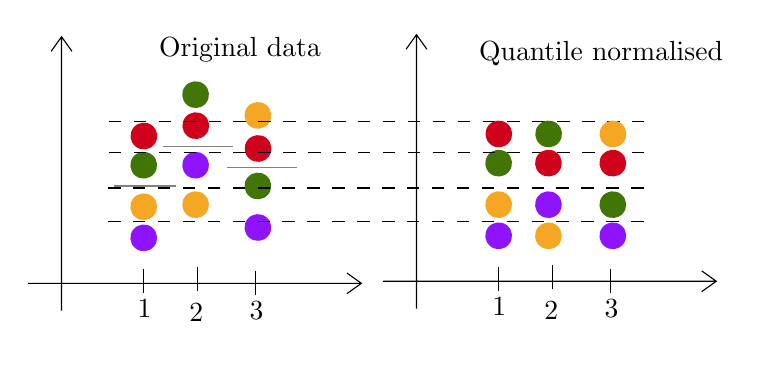
\begin{tikzpicture}[x=0.75pt,y=0.75pt,yscale=-1,xscale=1]
%uncomment if require: \path (0,195.33333206176758); %set diagram left start at 0, and has height of 195.33333206176758

%Shape: Axis 2D [id:dp4071697184363743] 
\draw  (31,131.8) -- (191.5,131.8)(47.05,13) -- (47.05,145) (184.5,126.8) -- (191.5,131.8) -- (184.5,136.8) (42.05,20) -- (47.05,13) -- (52.05,20)  ;
%Flowchart: Connector [id:dp47796321909784445] 
\draw  [draw opacity=0][fill={rgb, 255:red, 65; green, 117; blue, 5 }  ,fill opacity=1 ] (90.71,69.91) .. controls (87.96,67.66) and (83.9,68.07) .. (81.65,70.83) .. controls (79.4,73.59) and (79.81,77.64) .. (82.57,79.89) .. controls (85.33,82.14) and (89.39,81.73) .. (91.63,78.97) .. controls (93.88,76.21) and (93.47,72.16) .. (90.71,69.91) -- cycle ;
%Flowchart: Connector [id:dp775136720322851] 
\draw  [draw opacity=0][fill={rgb, 255:red, 144; green, 19; blue, 254 }  ,fill opacity=1 ] (90.71,104.91) .. controls (87.96,102.66) and (83.9,103.07) .. (81.65,105.83) .. controls (79.4,108.59) and (79.81,112.64) .. (82.57,114.89) .. controls (85.33,117.14) and (89.39,116.73) .. (91.63,113.97) .. controls (93.88,111.21) and (93.47,107.16) .. (90.71,104.91) -- cycle ;
%Flowchart: Connector [id:dp479825470074684] 
\draw  [draw opacity=0][fill={rgb, 255:red, 245; green, 166; blue, 35 }  ,fill opacity=1 ] (90.71,89.91) .. controls (87.96,87.66) and (83.9,88.07) .. (81.65,90.83) .. controls (79.4,93.59) and (79.81,97.64) .. (82.57,99.89) .. controls (85.33,102.14) and (89.39,101.73) .. (91.63,98.97) .. controls (93.88,96.21) and (93.47,92.16) .. (90.71,89.91) -- cycle ;
%Flowchart: Connector [id:dp8772408378730552] 
\draw  [draw opacity=0][fill={rgb, 255:red, 208; green, 2; blue, 27 }  ,fill opacity=1 ] (90.79,55.84) .. controls (88.03,53.6) and (83.98,54.01) .. (81.73,56.77) .. controls (79.48,59.52) and (79.89,63.58) .. (82.65,65.83) .. controls (85.41,68.08) and (89.46,67.66) .. (91.71,64.91) .. controls (93.96,62.15) and (93.55,58.09) .. (90.79,55.84) -- cycle ;
%Flowchart: Connector [id:dp7273952498995546] 
\draw  [draw opacity=0][fill={rgb, 255:red, 65; green, 117; blue, 5 }  ,fill opacity=1 ] (115.71,35.91) .. controls (112.96,33.66) and (108.9,34.07) .. (106.65,36.83) .. controls (104.4,39.59) and (104.81,43.64) .. (107.57,45.89) .. controls (110.33,48.14) and (114.39,47.73) .. (116.63,44.97) .. controls (118.88,42.21) and (118.47,38.16) .. (115.71,35.91) -- cycle ;
%Flowchart: Connector [id:dp21583380928952534] 
\draw  [draw opacity=0][fill={rgb, 255:red, 144; green, 19; blue, 254 }  ,fill opacity=1 ] (115.71,69.91) .. controls (112.96,67.66) and (108.9,68.07) .. (106.65,70.83) .. controls (104.4,73.59) and (104.81,77.64) .. (107.57,79.89) .. controls (110.33,82.14) and (114.39,81.73) .. (116.63,78.97) .. controls (118.88,76.21) and (118.47,72.16) .. (115.71,69.91) -- cycle ;
%Flowchart: Connector [id:dp367353299394227] 
\draw  [draw opacity=0][fill={rgb, 255:red, 245; green, 166; blue, 35 }  ,fill opacity=1 ] (115.71,88.91) .. controls (112.96,86.66) and (108.9,87.07) .. (106.65,89.83) .. controls (104.4,92.59) and (104.81,96.64) .. (107.57,98.89) .. controls (110.33,101.14) and (114.39,100.73) .. (116.63,97.97) .. controls (118.88,95.21) and (118.47,91.16) .. (115.71,88.91) -- cycle ;
%Flowchart: Connector [id:dp9918881154852264] 
\draw  [draw opacity=0][fill={rgb, 255:red, 208; green, 2; blue, 27 }  ,fill opacity=1 ] (115.79,50.84) .. controls (113.03,48.6) and (108.98,49.01) .. (106.73,51.77) .. controls (104.48,54.52) and (104.89,58.58) .. (107.65,60.83) .. controls (110.41,63.08) and (114.46,62.66) .. (116.71,59.91) .. controls (118.96,57.15) and (118.55,53.09) .. (115.79,50.84) -- cycle ;
%Flowchart: Connector [id:dp8737482771717215] 
\draw  [draw opacity=0][fill={rgb, 255:red, 65; green, 117; blue, 5 }  ,fill opacity=1 ] (145.71,79.91) .. controls (142.96,77.66) and (138.9,78.07) .. (136.65,80.83) .. controls (134.4,83.59) and (134.81,87.64) .. (137.57,89.89) .. controls (140.33,92.14) and (144.39,91.73) .. (146.63,88.97) .. controls (148.88,86.21) and (148.47,82.16) .. (145.71,79.91) -- cycle ;
%Flowchart: Connector [id:dp8886502638185938] 
\draw  [draw opacity=0][fill={rgb, 255:red, 144; green, 19; blue, 254 }  ,fill opacity=1 ] (145.71,99.91) .. controls (142.96,97.66) and (138.9,98.07) .. (136.65,100.83) .. controls (134.4,103.59) and (134.81,107.64) .. (137.57,109.89) .. controls (140.33,112.14) and (144.39,111.73) .. (146.63,108.97) .. controls (148.88,106.21) and (148.47,102.16) .. (145.71,99.91) -- cycle ;
%Flowchart: Connector [id:dp12839712018807292] 
\draw  [draw opacity=0][fill={rgb, 255:red, 245; green, 166; blue, 35 }  ,fill opacity=1 ] (145.71,45.91) .. controls (142.96,43.66) and (138.9,44.07) .. (136.65,46.83) .. controls (134.4,49.59) and (134.81,53.64) .. (137.57,55.89) .. controls (140.33,58.14) and (144.39,57.73) .. (146.63,54.97) .. controls (148.88,52.21) and (148.47,48.16) .. (145.71,45.91) -- cycle ;
%Flowchart: Connector [id:dp22911262187569625] 
\draw  [draw opacity=0][fill={rgb, 255:red, 208; green, 2; blue, 27 }  ,fill opacity=1 ] (145.79,61.84) .. controls (143.03,59.6) and (138.98,60.01) .. (136.73,62.77) .. controls (134.48,65.52) and (134.89,69.58) .. (137.65,71.83) .. controls (140.41,74.08) and (144.46,73.66) .. (146.71,70.91) .. controls (148.96,68.15) and (148.55,64.09) .. (145.79,61.84) -- cycle ;
%Straight Lines [id:da7437423031647632] 
\draw    (140.63,126) -- (140.63,137.3) ;


%Straight Lines [id:da3500611217714251] 
\draw    (112.63,124) -- (112.63,135.3) ;


%Straight Lines [id:da4946427268334965] 
\draw    (86.63,125) -- (86.63,136.3) ;


%Straight Lines [id:da39022019683066134] 
\draw [color={rgb, 255:red, 128; green, 128; blue, 128 }  ,draw opacity=1 ]   (126.96,75.91) -- (160.46,75.91) ;


%Straight Lines [id:da3674903648864307] 
\draw [color={rgb, 255:red, 128; green, 128; blue, 128 }  ,draw opacity=1 ]   (95.96,65.91) -- (129.46,65.91) ;


%Straight Lines [id:da08905855224756842] 
\draw [color={rgb, 255:red, 128; green, 128; blue, 128 }  ,draw opacity=1 ]   (72.5,84.89) -- (102.32,84.89) ;


%Straight Lines [id:da8838665914886257] 
\draw  [dash pattern={on 4.5pt off 4.5pt}]  (69.89,53.9) -- (330.83,53.9) ;


%Shape: Axis 2D [id:dp5094712129345804] 
\draw  (202,130.8) -- (362.5,130.8)(218.05,12) -- (218.05,144) (355.5,125.8) -- (362.5,130.8) -- (355.5,135.8) (213.05,19) -- (218.05,12) -- (223.05,19)  ;
%Flowchart: Connector [id:dp9701135659715163] 
\draw  [draw opacity=0][fill={rgb, 255:red, 65; green, 117; blue, 5 }  ,fill opacity=1 ] (261.71,68.91) .. controls (258.96,66.66) and (254.9,67.07) .. (252.65,69.83) .. controls (250.4,72.59) and (250.81,76.64) .. (253.57,78.89) .. controls (256.33,81.14) and (260.39,80.73) .. (262.63,77.97) .. controls (264.88,75.21) and (264.47,71.16) .. (261.71,68.91) -- cycle ;
%Flowchart: Connector [id:dp19815624460829806] 
\draw  [draw opacity=0][fill={rgb, 255:red, 144; green, 19; blue, 254 }  ,fill opacity=1 ] (261.71,103.91) .. controls (258.96,101.66) and (254.9,102.07) .. (252.65,104.83) .. controls (250.4,107.59) and (250.81,111.64) .. (253.57,113.89) .. controls (256.33,116.14) and (260.39,115.73) .. (262.63,112.97) .. controls (264.88,110.21) and (264.47,106.16) .. (261.71,103.91) -- cycle ;
%Flowchart: Connector [id:dp5444970436061509] 
\draw  [draw opacity=0][fill={rgb, 255:red, 245; green, 166; blue, 35 }  ,fill opacity=1 ] (261.71,88.91) .. controls (258.96,86.66) and (254.9,87.07) .. (252.65,89.83) .. controls (250.4,92.59) and (250.81,96.64) .. (253.57,98.89) .. controls (256.33,101.14) and (260.39,100.73) .. (262.63,97.97) .. controls (264.88,95.21) and (264.47,91.16) .. (261.71,88.91) -- cycle ;
%Flowchart: Connector [id:dp4129473941443531] 
\draw  [draw opacity=0][fill={rgb, 255:red, 208; green, 2; blue, 27 }  ,fill opacity=1 ] (261.79,54.84) .. controls (259.03,52.6) and (254.98,53.01) .. (252.73,55.77) .. controls (250.48,58.52) and (250.89,62.58) .. (253.65,64.83) .. controls (256.41,67.08) and (260.46,66.66) .. (262.71,63.91) .. controls (264.96,61.15) and (264.55,57.09) .. (261.79,54.84) -- cycle ;
%Straight Lines [id:da49630299738040096] 
\draw    (311.63,125) -- (311.63,136.3) ;


%Straight Lines [id:da3409139232705698] 
\draw    (283.63,123) -- (283.63,134.3) ;


%Straight Lines [id:da9094998541395087] 
\draw    (257.63,124) -- (257.63,135.3) ;


%Straight Lines [id:da2261043426810294] 
\draw  [dash pattern={on 4.5pt off 4.5pt}]  (69.89,68.9) -- (330.83,68.9) ;


%Straight Lines [id:da5824626395640147] 
\draw  [dash pattern={on 4.5pt off 4.5pt}]  (69.5,85.89) -- (330.44,85.89) ;


%Straight Lines [id:da7047611196217718] 
\draw  [dash pattern={on 4.5pt off 4.5pt}]  (69.5,101.89) -- (330.44,101.89) ;


%Flowchart: Connector [id:dp8893219442781508] 
\draw  [draw opacity=0][fill={rgb, 255:red, 208; green, 2; blue, 27 }  ,fill opacity=1 ] (285.71,68.91) .. controls (282.96,66.66) and (278.9,67.07) .. (276.65,69.83) .. controls (274.4,72.59) and (274.81,76.64) .. (277.57,78.89) .. controls (280.33,81.14) and (284.39,80.73) .. (286.63,77.97) .. controls (288.88,75.21) and (288.47,71.16) .. (285.71,68.91) -- cycle ;
%Flowchart: Connector [id:dp3959621528301924] 
\draw  [draw opacity=0][fill={rgb, 255:red, 245; green, 166; blue, 35 }  ,fill opacity=1 ] (285.71,103.91) .. controls (282.96,101.66) and (278.9,102.07) .. (276.65,104.83) .. controls (274.4,107.59) and (274.81,111.64) .. (277.57,113.89) .. controls (280.33,116.14) and (284.39,115.73) .. (286.63,112.97) .. controls (288.88,110.21) and (288.47,106.16) .. (285.71,103.91) -- cycle ;
%Flowchart: Connector [id:dp1772629821607905] 
\draw  [draw opacity=0][fill={rgb, 255:red, 144; green, 19; blue, 254 }  ,fill opacity=1 ] (285.71,88.91) .. controls (282.96,86.66) and (278.9,87.07) .. (276.65,89.83) .. controls (274.4,92.59) and (274.81,96.64) .. (277.57,98.89) .. controls (280.33,101.14) and (284.39,100.73) .. (286.63,97.97) .. controls (288.88,95.21) and (288.47,91.16) .. (285.71,88.91) -- cycle ;
%Flowchart: Connector [id:dp852667519103441] 
\draw  [draw opacity=0][fill={rgb, 255:red, 65; green, 117; blue, 5 }  ,fill opacity=1 ] (285.79,54.84) .. controls (283.03,52.6) and (278.98,53.01) .. (276.73,55.77) .. controls (274.48,58.52) and (274.89,62.58) .. (277.65,64.83) .. controls (280.41,67.08) and (284.46,66.66) .. (286.71,63.91) .. controls (288.96,61.15) and (288.55,57.09) .. (285.79,54.84) -- cycle ;
%Flowchart: Connector [id:dp42164729435747383] 
\draw  [draw opacity=0][fill={rgb, 255:red, 208; green, 2; blue, 27 }  ,fill opacity=1 ] (316.71,68.91) .. controls (313.96,66.66) and (309.9,67.07) .. (307.65,69.83) .. controls (305.4,72.59) and (305.81,76.64) .. (308.57,78.89) .. controls (311.33,81.14) and (315.39,80.73) .. (317.63,77.97) .. controls (319.88,75.21) and (319.47,71.16) .. (316.71,68.91) -- cycle ;
%Flowchart: Connector [id:dp1353268144862132] 
\draw  [draw opacity=0][fill={rgb, 255:red, 144; green, 19; blue, 254 }  ,fill opacity=1 ] (316.71,103.91) .. controls (313.96,101.66) and (309.9,102.07) .. (307.65,104.83) .. controls (305.4,107.59) and (305.81,111.64) .. (308.57,113.89) .. controls (311.33,116.14) and (315.39,115.73) .. (317.63,112.97) .. controls (319.88,110.21) and (319.47,106.16) .. (316.71,103.91) -- cycle ;
%Flowchart: Connector [id:dp5695947224831286] 
\draw  [draw opacity=0][fill={rgb, 255:red, 65; green, 117; blue, 5 }  ,fill opacity=1 ] (316.71,88.91) .. controls (313.96,86.66) and (309.9,87.07) .. (307.65,89.83) .. controls (305.4,92.59) and (305.81,96.64) .. (308.57,98.89) .. controls (311.33,101.14) and (315.39,100.73) .. (317.63,97.97) .. controls (319.88,95.21) and (319.47,91.16) .. (316.71,88.91) -- cycle ;
%Flowchart: Connector [id:dp5282331948658441] 
\draw  [draw opacity=0][fill={rgb, 255:red, 245; green, 166; blue, 35 }  ,fill opacity=1 ] (316.79,54.84) .. controls (314.03,52.6) and (309.98,53.01) .. (307.73,55.77) .. controls (305.48,58.52) and (305.89,62.58) .. (308.65,64.83) .. controls (311.41,67.08) and (315.46,66.66) .. (317.71,63.91) .. controls (319.96,61.15) and (319.55,57.09) .. (316.79,54.84) -- cycle ;

% Text Node
\draw (87,144) node   [align=left] {1};
% Text Node
\draw (112,154) node   [align=left] {2\\};
% Text Node
\draw (141,145) node   [align=left] {3};
% Text Node
\draw (258,143) node   [align=left] {1};
% Text Node
\draw (283,153) node   [align=left] {2\\};
% Text Node
\draw (312,144) node   [align=left] {3};
% Text Node
\draw (307,21) node   [align=left] {Quantile normalised};
% Text Node
\draw (133,19) node   [align=left] {Original data};


\end{tikzpicture}

The idea for quantile normalisation ressembles the offset in linear regression. You account for differences in samples to adequately compare them.
\begin{enumerate}
	\item[]	 To compensate for the differences in lightbulb intensity across samples, want to normalise the data points; you can see the difference in means across all three \textcolor{gray}{in gray}.
	\item	Focus on the maximum value of each sample and take the mean.
	\item[]	Extend this mean onto the new plot and that becomes the new value for all 3 samples.
	\item	Repeat for all the points.
	\item[]	The end result is that the \textbf{values are all the same} but the \textbf{order of the colours is maintained} enabling an adequate comparison.
\end{enumerate}
\end{YTB_SUMM}

\newpage
\chapter[Linear Models]{Linear Models (40\% à 50\%)}

\subsubsection{Information}

\begin{distributions}[Objective]
Understand key concepts concerning Generalized Linear Models
\end{distributions}

\begin{outcomes}[Learning outcomes]
\begin{enumerate}
	\item	Décrire et expliquer les composantes de la famille exponentielle et des fonctions de lien.
	\item	Estimer les paramètres par Least Squares et maximum de vraisemblance.
	\item	Interpréter les tests de vérification pour l'ajustement de modèle et la vérification des postulats graphiquement et numériquement.
	\item	Sélectionner un modèle approprié en prenant en compte:
	\begin{itemize}
		\item	Distributions et fonctions de lien
		\item	Transformations de variables, et leurs interactions
		\item	Statistique (du khi-carré) de Pearson
		\item	Tests $t$ et $F$
		\item	AIC et BIC
		\item	Test du Rapport de Vraisemblance (TRV)
	\end{itemize}
	\item	Interpréter les résultats du modèle dans le cadre de son utilisation pour résoudre aux problèmes d'affaires sous-jacents
	\item	Calculer et interpréter les valeurs prédites ainsi que les intervalles de confiance et de prévision.
	\item	Comprendre que d'autres méthodes peuvent différer du modèle OLS comme la régression Lasso, Ridge et KNN.
\end{enumerate}
\end{outcomes}

\begin{ASM_chapter}[Related lessons ASM]
\begin{enumerate}
  \setcounter{enumi}{1}
	\item	\hyperref[LM-ESTIMATION]{Linear Regression:  Estimating parameters}
	\item	\hyperref[LM-STDERROR]{Linear Regression:  Standard Error, $R^{2}$, and $t$ statistic}
	\item	\hyperref[LM-F]{Linear Regression:  $F$ statistic}
	\tcbline
	\item	\hyperref[VALID-VALID]{Linear Regression:  Validation}
	\item	\hyperref[VALID-RESAMPLING]{Resampling methods}
	\item	\hyperref[VALID-SUBSETS]{Linear Regression:  Subset Selection}
	\item	\hyperref[VALID-SHRINKAGE]{Linear Regression:  Shrinkage and Dimension Reduction}
	\tcbline
	\item	\hyperref[PREV-PREDICTIONS]{Linear Regression:  Predictions}
	\item	\hyperref[PREV-INTERP]{Interpreting Regression Results}
	\tcbline
	\item	\hyperref[GLM-BASICS]{Generalized Linear Models:  Basics}
	\item	\hyperref[GLM-CAT]{Generalized Linear Models:  Categorical Response}
	\item	\hyperref[GLM-COUNT]{Generalized Linear Models:  Count Response}
	\item	\hyperref[GLM-MEZ-FIT]{Generalized Linear Models:  Measures of Fit}
	\tcbline
	\item	\hyperref[PCA-KNN]{PCA: $K$-Nearest neighbors}
\end{enumerate}
\end{ASM_chapter}

\begin{YTB_vids}[Vidéos YouTube]
\begin{itemize}
	\item	\href{https://www.youtube.com/watch?v=2QeDRsxSF9M&t=369s}{Khan Academy: Pearson's chi square test (goodness of fit)}
	\item	\href{https://www.youtube.com/watch?v=PaFPbb66DxQ&list=PLblh5JKOoLUIzaEkCLIUxQFjPIlapw8nU&index=1}{StatQuest: Fitting a line to data, aka least squares, aka linear regression}
	\item	\href{https://www.youtube.com/watch?v=2AQKmw14mHM&list=PLblh5JKOoLUIzaEkCLIUxQFjPIlapw8nU&index=10}{StatQuest: R-squared explained}
	\item	\href{https://www.youtube.com/watch?v=nk2CQITm_eo&list=PLblh5JKOoLUIzaEkCLIUxQFjPIlapw8nU&index=2}{StatQuest: Linear Models Pt.1 - Linear Regression}
	\item	\href{https://www.youtube.com/watch?v=u1cc1r_Y7M0&list=PLblh5JKOoLUIzaEkCLIUxQFjPIlapw8nU&index=3}{StatQuest: Linear Regression in R}
	\item	\href{https://www.youtube.com/watch?v=zITIFTsivN8&list=PLblh5JKOoLUIzaEkCLIUxQFjPIlapw8nU&index=5}{StatQuest: Linear Models Pt.1.5 - Multiple Regression}
	\item	\href{https://www.youtube.com/watch?v=hokALdIst8k}{StatQuest: Multiple Regression in R}
	\item	\href{https://www.youtube.com/watch?v=NF5_btOaCig&list=PLblh5JKOoLUIzaEkCLIUxQFjPIlapw8nU&index=6}{StatQuest: Linear Models Pt.2 - t-tests and ANOVA}
	\item	\href{https://www.youtube.com/watch?v=CqLGvwi-5Pc&list=PLblh5JKOoLUIzaEkCLIUxQFjPIlapw8nU&index=7}{StatQuest: Linear Models Pt.3 - Design Matrices}
	\item	\href{https://www.youtube.com/watch?v=Hrr2anyK_5s&list=PLblh5JKOoLUIzaEkCLIUxQFjPIlapw8nU&index=8}{StatQuest: Linear Models Pt.3 - Design Matrix Examples in R}
	\tcbline
	\item	\href{https://www.youtube.com/watch?v=Z-jXJpVohiI}{Phil Chan: Introduction to the Hat matrix in regression}
	\item	\href{https://www.youtube.com/watch?v=eY-uOXQPXm8}{Phil Chan: Properties of the Hat matrix with proofs} \textit{(pas pertinent pour SRM, pas regarder dans ce cadre.)}
	\item	\href{https://www.youtube.com/watch?v=l2xG_yehq0k&t=146s}{Phil Chan: How is it the Hat matrix spans the column space of X? Really nice.}
	\item	\href{https://www.youtube.com/watch?v=-yIF_TXc6h0&t=96s}{Phil Chan: What does it mean to say the Hat matrix is an orthogonal projection?} \textit{(pas pertinent pour SRM, pas regarder dans ce cadre; pas encore regardé moi-même mais je le note comme référence.)}
	\item	\href{https://www.youtube.com/watch?v=UyAa5iwJ7m0&list=PLe0nS0mZ7vGGhYcDPNSVNu9gT3wGHbjhu&index=3}{Phil Chan: Should I look at raw, standardized, or studentized residuals? part 1 - what to look out for}
	\item	\href{https://www.youtube.com/watch?v=UyAa5iwJ7m0&list=PLe0nS0mZ7vGGhYcDPNSVNu9gT3wGHbjhu&index=4}{Phil Chan: Should I look at raw, standardized, or studentized residuals? part 2 - kinds of residuals}
	\item	\href{https://www.youtube.com/watch?v=mEdSj3wlN4Q}{Phil Chan: Should I look at raw, standardized, or studentized residuals? part 3}
	\item	\href{https://www.youtube.com/watch?v=s5X_Poq9dJA}{Phil Chan: What's the difference between an outlier and a leverage point in regression?}
	\item	\href{https://www.youtube.com/watch?v=31xA3hsxW6k}{Phil Chan: Influential points - Cook's distance, DFFITS, DFBETAS}
	\item	\href{https://www.youtube.com/watch?v=xc_X9GFVuVU&t=6m20s}{jbstatistics: Leverage and Influential Points in Simple Linear Regression} (\textit{didn't watch the whole thing because time, but he breaks down the formula for leverage very well towards the end})
	\item	\href{https://www.youtube.com/watch?v=0SBIXgPVex8}{Ben Lambert: Variance Inflation Factors: testing for multicollinearity}
	\item	\href{https://www.youtube.com/watch?v=fSytzGwwBVw}{StatQuest: Machine Learning Fundamentals: Cross Validation}
	\item	\href{https://www.youtube.com/watch?v=KjRrdb2x6dA}{Stephanie Glen: Adjusted R Squared}
	\item	\href{https://www.youtube.com/watch?v=8W2fGkU5LYU}{Ben Lambert: Adjusted R squared}
	\item	\href{https://www.youtube.com/watch?v=5fN2J8wYnfw}{ritvikmath: Vector Norms}
	\item	\href{https://www.youtube.com/watch?v=Q81RR3yKn30&list=PLblh5JKOoLUICTaGLRoHQDuF_7q2GfuJF}{StatQuest: Regularization Part 1: Ridge Regression}
	\item	\href{https://www.youtube.com/watch?v=NGf0voTMlcs&list=PLblh5JKOoLUICTaGLRoHQDuF_7q2GfuJF}{StatQuest: Regularization Part 2: Lasso Regression}
	\tcbline
	\item	\href{https://www.youtube.com/watch?v=yIYKR4sgzI8}{StatQuest: Logistic Regression}
	\item	\href{https://www.youtube.com/watch?v=pYxNSUDSFH4&feature=youtu.be}{StatQuest: Probability vs Likelihood}
	\item	\href{https://www.youtube.com/watch?v=XepXtl9YKwc&feature=youtu.be}{StatQuest: Maximum Likelihood, clearly explained!!!}
	\item[]
	\begin{distributions}[Pas regardé les 6 suivants mais je me les note comme référence au cas où que j'aurai le temps]
	\item	\href{https://www.youtube.com/watch?v=Dn6b9fCIUpM}{StatQuest: Maximum Likelihood For the Normal Distribution, step-by-step!}
	\item	\href{https://www.youtube.com/watch?v=p3T-_LMrvBc}{StatQuest: Maximum Likelihood for the Exponential Distribution, Clearly Explained! V2.0}
	\item	\href{https://www.youtube.com/watch?v=4KKV9yZCoM4}{StatQuest: Maximum Likelihood for the Binomial Distribution, Clearly Explained!!!}
	\item	\href{https://www.youtube.com/watch?v=vN5cNN2-HWE&feature=youtu.be}{StatQuest: Logistic Regression Details Pt1: Coefficients}
	\item	\href{https://www.youtube.com/watch?v=BfKanl1aSG0&feature=youtu.be}{Logistic Regression Details Pt 2: Maximum Likelihood}
	\item	\href{https://www.youtube.com/watch?v=xxFYro8QuXA&feature=youtu.be}{Logistic Regression Details Pt 3: R-squared and p-value}
	\end{distributions}
	\item	\href{https://www.youtube.com/watch?v=ARfXDSkQf1Y}{StatQuest: Odds and Log(Odds), Clearly Explained!!!}
	\item	\href{https://www.youtube.com/watch?v=8nm0G-1uJzA}{StatQuest: Odds Ratios and Log(Odds Ratios), Clearly Explained!!!}
	\tcbline
	\item	\href{https://www.youtube.com/watch?v=HVXime0nQeI&list=PLblh5JKOoLUICTaGLRoHQDuF_7q2GfuJF&index=33}{StatQuest: K-nearest neighbors, Clearly Explained}
\end{itemize}
\end{YTB_vids}

\section{Régression linéaire}

\subsection{Résumés des chapitres}

\begin{CHPT_SUMM}[label = {LM-ESTIMATION}]{\addcontentsline{toc}{subsubsection}{2. Linear Regression:  Estimating parameters}2. Linear Regression:  Estimating parameters}
\begin{enumerate}
	\item	Régression linéaire simple
	\begin{itemize}
		\item	Hypothèses pour les résidus;
		\item	Différentes formulations des estimateurs. Particulièrement, d'exprimer $\hat\beta_{1}$ en fonction du coefficient de corrélation, la covariance et les variances échantillonnalles.
	\end{itemize}
	\item	Régression linéaire multiple
	\begin{itemize}
		\item	Faire attention à la colinéarité;
		\item	Idée de ne pas avoir une colonne qui somme à un sinon intéraction avec la rangée de 1.
	\end{itemize}
	\item	Généralisations de régression linéaire
	\begin{itemize}
		\item	Régression linéaire pondérée;
		\item	Transformation (exposant, polynomiale, log, ...);
		\item	Famille de transformations Box-Cox.
	\end{itemize}
\end{enumerate}
\textbf{Note sur les exercices:} Généralement 2 types
\begin{enumerate}
	\item	Trouver estimations de $\hat\beta_{1}$ pour une régression linéaire simple;
	\item	Trouver estimations de $\hat\beta_{1}$ pour une régression linéaire multiple.
\end{enumerate}
Dans les deux cas c'est à partir de données qui incluent souvent le produit croisée des observations, ou la corrélation, etc.
\end{CHPT_SUMM}

\begin{CHPT_SUMM}[label = {LM-STDERROR}]{\addcontentsline{toc}{subsubsection}{3. Linear Regression: Standard Error\, $R^{2}$\, and $t$ statistic}3. Linear Regression: Standard Error\, $R^{2}$\, and $t$ statistic}
\begin{enumerate}
	\item	Residual Standard Error of the Regression
	\begin{itemize}
		\item	Bien distinguer toutes les différentes façons de dire et d'écrire les équations pour les sommes des carrées.
	\end{itemize}
	\item	$R^{2}$: Coefficient de détermination
	\begin{itemize}
		\item	Savoir les différentes façon de l'écrire afin d'être en mesure de le calculer à partir d'une variété d'information donnée.
	\end{itemize}
	\item	Statistique $t$
	\item	Graphique et algorithme de variable ajoutée et coefficient de corrélation partiel
	\begin{itemize}
		\item	Remember the algorithm for the added-variable plot (p.31)
		\item	Remember the formula for the partial correlation coefficient $\frac{t(b_{1})}{\sqrt{t(b_{1})^{2} + (n - p')}}$.
	\end{itemize}
\end{enumerate}
\textbf{Note sur les exercices:} Généralement de 3 à 4 types:
\begin{enumerate}
	\item	Trouver le $R^{2}$, MSE, etc. à partir d'information donnée; donc savoir les différentes formulations pour ces équations;
	\item	Trouver les statistiques t pour les paramètres;
	\item	Trouver des intervalles de confiance pour les paramètres;
	\item	Peut-être une sur le coefficient de corrélation mais c'est facile à trouver.
\end{enumerate}
Donc il faut concrètement comprendre la distinction et les formules pour les SS, $R^{2}$ et variance des coefficients.
\end{CHPT_SUMM}

\begin{CHPT_SUMM}[label = {LM-F}]{\addcontentsline{toc}{subsubsection}{4. Linear Regression: $F$ statistic}4. Linear Regression: $F$ statistic}
En gros le chapitre explique les deux différents tests F
\begin{enumerate}
	\item	Test de la validité gloable que l'on compare notre modèle à la moyenne.
	\begin{itemize}
		\item	Voir les vidéos de StatQuest, il couvre les tests F en expliquant le reste de la régression linéaire.
		\item	Savoir que pour un test du retrait d'une seule variable $\beta_{1}$, $F_{1, n - 2} = (t_{n - 2})^{2}$.
		\item	Savoir la connection avec le $R^{2}$ en divisant par le SST.
	\end{itemize}
	\item	Test pour le retrait de variables.
	\begin{itemize}
		\item	Également lien avec le $R^{2}$.
		\item	Faire attention au degrés de liberté si on donne les MSE pour les deux modèles; pas le même pour les deux.
	\end{itemize}
\end{enumerate}
\textbf{Note sur les exercices:} Généralement de 2 types:
\begin{enumerate}
	\item	Trouver la statistique F pour le test global;
	\item	Trouver la statistique F pour le test partiel. 
\end{enumerate}
Dans les deux cas, souvent la question donne de l'information partielle et il faut savoir utiliser les différentes formulations pour l'équation. Pour exemple, avec $R^{2}$, avec le $t^{2}$, avec SSR ou SSE, etc.
\end{CHPT_SUMM}

\subsection{Notes sur les vidéos YouTube}


\begin{YTB_SUMM}{\href{https://www.youtube.com/watch?v=PaFPbb66DxQ&list=PLblh5JKOoLUIzaEkCLIUxQFjPIlapw8nU&index=1}{StatQuest: Fitting a line to data, aka least squares, aka linear regression}}
Recall the basic formula $y = ax + b$.
\begin{enumerate}
	\item	In Least Squares, we want to find the starting point on the line ($b$ or $\beta_0$) and the slope ($a$ or $\beta_1$) to minimise the distance of the points to the line.
\end{enumerate}
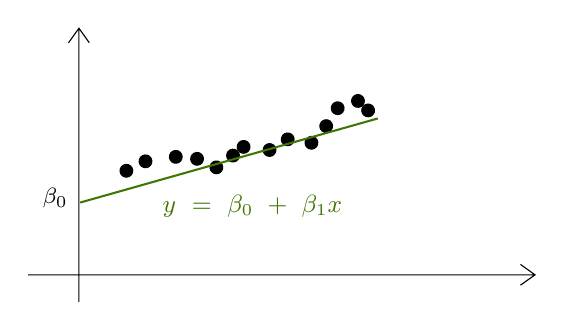
\begin{tikzpicture}[x=0.75pt,y=0.75pt,yscale=-1,xscale=1]
%uncomment if require: \path (0,195.33333206176758); %set diagram left start at 0, and has height of 195.33333206176758

%Shape: Axis 2D [id:dp35721852247943175] 
\draw  (31,131.8) -- (275.17,131.8)(55.42,13) -- (55.42,145) (268.17,126.8) -- (275.17,131.8) -- (268.17,136.8) (50.42,20) -- (55.42,13) -- (60.42,20)  ;
%Flowchart: Connector [id:dp7405838412090233] 
\draw  [fill={rgb, 255:red, 0; green, 0; blue, 0 }  ,fill opacity=1 ] (110.41,78.3) .. controls (109.09,77.23) and (108.9,75.3) .. (109.97,73.99) .. controls (111.04,72.68) and (112.96,72.49) .. (114.28,73.56) .. controls (115.59,74.62) and (115.78,76.55) .. (114.71,77.86) .. controls (113.65,79.17) and (111.72,79.37) .. (110.41,78.3) -- cycle ;
%Flowchart: Connector [id:dp4208481249614251] 
\draw  [fill={rgb, 255:red, 0; green, 0; blue, 0 }  ,fill opacity=1 ] (85.57,79.5) .. controls (84.26,78.43) and (84.06,76.5) .. (85.13,75.19) .. controls (86.2,73.88) and (88.13,73.69) .. (89.44,74.75) .. controls (90.75,75.82) and (90.95,77.75) .. (89.88,79.06) .. controls (88.81,80.37) and (86.88,80.57) .. (85.57,79.5) -- cycle ;
%Flowchart: Connector [id:dp7170407416997207] 
\draw  [fill={rgb, 255:red, 0; green, 0; blue, 0 }  ,fill opacity=1 ] (145.33,74.04) .. controls (144.02,72.97) and (143.82,71.05) .. (144.89,69.73) .. controls (145.96,68.42) and (147.89,68.23) .. (149.2,69.3) .. controls (150.51,70.36) and (150.71,72.29) .. (149.64,73.6) .. controls (148.57,74.91) and (146.64,75.11) .. (145.33,74.04) -- cycle ;
%Flowchart: Connector [id:dp9831981842904083] 
\draw  [fill={rgb, 255:red, 0; green, 0; blue, 0 }  ,fill opacity=1 ] (127.73,76.73) .. controls (126.42,75.66) and (126.22,73.73) .. (127.29,72.42) .. controls (128.36,71.11) and (130.29,70.92) .. (131.6,71.98) .. controls (132.91,73.05) and (133.1,74.98) .. (132.04,76.29) .. controls (130.97,77.6) and (129.04,77.8) .. (127.73,76.73) -- cycle ;
%Flowchart: Connector [id:dp6597419850766411] 
\draw  [fill={rgb, 255:red, 0; green, 0; blue, 0 }  ,fill opacity=1 ] (192.81,54.97) .. controls (191.5,53.9) and (191.3,51.97) .. (192.37,50.66) .. controls (193.44,49.35) and (195.37,49.15) .. (196.68,50.22) .. controls (197.99,51.29) and (198.19,53.22) .. (197.12,54.53) .. controls (196.05,55.84) and (194.12,56.04) .. (192.81,54.97) -- cycle ;
%Flowchart: Connector [id:dp12644057862139046] 
\draw  [fill={rgb, 255:red, 0; green, 0; blue, 0 }  ,fill opacity=1 ] (165.51,70.57) .. controls (164.2,69.5) and (164,67.57) .. (165.07,66.26) .. controls (166.14,64.95) and (168.07,64.75) .. (169.38,65.82) .. controls (170.69,66.89) and (170.89,68.82) .. (169.82,70.13) .. controls (168.75,71.44) and (166.82,71.63) .. (165.51,70.57) -- cycle ;
%Flowchart: Connector [id:dp9469181871169179] 
\draw  [fill={rgb, 255:red, 0; green, 0; blue, 0 }  ,fill opacity=1 ] (172.62,62.54) .. controls (171.31,61.47) and (171.11,59.54) .. (172.18,58.23) .. controls (173.25,56.92) and (175.18,56.72) .. (176.49,57.79) .. controls (177.8,58.86) and (178,60.79) .. (176.93,62.1) .. controls (175.86,63.41) and (173.93,63.6) .. (172.62,62.54) -- cycle ;
%Flowchart: Connector [id:dp7748779153505232] 
\draw  [fill={rgb, 255:red, 0; green, 0; blue, 0 }  ,fill opacity=1 ] (154.07,68.91) .. controls (152.76,67.84) and (152.57,65.91) .. (153.64,64.6) .. controls (154.71,63.29) and (156.63,63.09) .. (157.94,64.16) .. controls (159.26,65.23) and (159.45,67.16) .. (158.38,68.47) .. controls (157.31,69.78) and (155.39,69.98) .. (154.07,68.91) -- cycle ;
%Flowchart: Connector [id:dp5494330788804085] 
\draw  [fill={rgb, 255:red, 0; green, 0; blue, 0 }  ,fill opacity=1 ] (76.36,84.06) .. controls (75.05,82.99) and (74.85,81.06) .. (75.92,79.75) .. controls (76.99,78.44) and (78.92,78.25) .. (80.23,79.31) .. controls (81.54,80.38) and (81.74,82.31) .. (80.67,83.62) .. controls (79.6,84.93) and (77.67,85.13) .. (76.36,84.06) -- cycle ;
%Flowchart: Connector [id:dp5890644622068899] 
\draw  [fill={rgb, 255:red, 0; green, 0; blue, 0 }  ,fill opacity=1 ] (100.16,77.35) .. controls (98.85,76.28) and (98.65,74.35) .. (99.72,73.04) .. controls (100.79,71.73) and (102.72,71.53) .. (104.03,72.6) .. controls (105.34,73.67) and (105.53,75.6) .. (104.46,76.91) .. controls (103.4,78.22) and (101.47,78.42) .. (100.16,77.35) -- cycle ;
%Flowchart: Connector [id:dp10183370135658154] 
\draw  [fill={rgb, 255:red, 0; green, 0; blue, 0 }  ,fill opacity=1 ] (119.71,82.41) .. controls (118.4,81.35) and (118.2,79.42) .. (119.27,78.11) .. controls (120.34,76.8) and (122.27,76.6) .. (123.58,77.67) .. controls (124.89,78.74) and (125.09,80.67) .. (124.02,81.98) .. controls (122.95,83.29) and (121.02,83.48) .. (119.71,82.41) -- cycle ;
%Flowchart: Connector [id:dp13579805852853988] 
\draw  [fill={rgb, 255:red, 0; green, 0; blue, 0 }  ,fill opacity=1 ] (132.83,72.55) .. controls (131.52,71.48) and (131.32,69.55) .. (132.39,68.24) .. controls (133.46,66.93) and (135.39,66.74) .. (136.7,67.81) .. controls (138.01,68.87) and (138.2,70.8) .. (137.13,72.11) .. controls (136.07,73.42) and (134.14,73.62) .. (132.83,72.55) -- cycle ;
%Flowchart: Connector [id:dp1916741178210739] 
\draw  [fill={rgb, 255:red, 0; green, 0; blue, 0 }  ,fill opacity=1 ] (178.15,53.91) .. controls (176.84,52.84) and (176.64,50.92) .. (177.71,49.61) .. controls (178.78,48.29) and (180.71,48.1) .. (182.02,49.17) .. controls (183.33,50.24) and (183.53,52.16) .. (182.46,53.47) .. controls (181.39,54.79) and (179.46,54.98) .. (178.15,53.91) -- cycle ;
%Flowchart: Connector [id:dp17036893605725] 
\draw  [fill={rgb, 255:red, 0; green, 0; blue, 0 }  ,fill opacity=1 ] (187.94,50.41) .. controls (186.62,49.34) and (186.43,47.41) .. (187.5,46.1) .. controls (188.57,44.79) and (190.49,44.59) .. (191.8,45.66) .. controls (193.12,46.73) and (193.31,48.66) .. (192.24,49.97) .. controls (191.17,51.28) and (189.25,51.48) .. (187.94,50.41) -- cycle ;
%Straight Lines [id:da2624274909662574] 
\draw [color={rgb, 255:red, 65; green, 117; blue, 5 }  ,draw opacity=1 ][line width=0.75]    (56.05,96.98) -- (199.41,56.48) ;



% Text Node
\draw (44,95) node  [font=\footnotesize] [align=left] {$\displaystyle \beta _{0}$};
% Text Node
\draw (139,99) node  [font=\small,color={rgb, 255:red, 65; green, 117; blue, 5 }  ,opacity=1 ] [align=left] {$\displaystyle y\ =\ \beta _{0} \ +\ \beta _{1} x$};


\end{tikzpicture}
\begin{enumerate}
  \setcounter{enumi}{1}
	\item	The distance of the points to the line are the \textbf{residuals} $\varepsilon$.
	\item	When we plot the SSR for the different possible curve, we pick the one with the \textit{smallest SSR}. 
	\begin{itemize}
		\item	That is to say, we pick the one with the \textbf{Least Squares}.
		\item 	That curve is the curve such that the derivative has a slope of 0 and it becomes the \textbf{Least Squares Estimator}.
	\end{itemize}
\end{enumerate}
\end{YTB_SUMM}

\begin{YTB_SUMM}{\href{https://www.youtube.com/watch?v=2AQKmw14mHM&list=PLblh5JKOoLUIzaEkCLIUxQFjPIlapw8nU&index=10}{StatQuest: R-squared explained}}
For comprehension, we define the measure of correlation by $R$ rather than $\rho$.
\begin{enumerate}
	\item	The main idea to retain is that $R^{2}$ is a \textbf{metric of correlation}.
	\item	In fact, $R^{2}$ is literally the \textbf{correlation squared},  $R^{2} = (R)^{2}$.
	\begin{itemize}
		\item	The advantage is that it's much easier to interpret and to calculate.
		\item	It's not obvious that $R = 0.7$ is twice as good as $R = 0.5$ but $R^{2} = 0.7^{2} = 0.5$ is clearly twice as good as $R^{2} = 0.5^{2} = 0.25$.
	\end{itemize}
	\item	The same idea from the Least Squares video is used, we want the line that will minimise the SSR. Now however, we want to \textbf{quantify how good} this new \textbf{line is} and we use the $R^{2}$.
	\item	$R^{2} = \frac{\text{Var}(\text{mean}) - \text{Var}(\text{Least Squares line})}{\text{Var}(\text{mean})}$. 
	\begin{itemize}
		\item	That is to say we divide the difference in the variation of the points to the line (SSR) by the variation of the points to the line that goes through the mean;
		\item	Thereby, this has to be between 0 and 1 since the SSR for any line is $\le$ SSR for the line going through the mean;
		\item	Thus $0 \le R^{2} \le 1$ and it is a percentage.
	\end{itemize}
	\item	The interpretation of $R^{2}$ can be either:
	\begin{itemize}
		\item	There is 81\% less variation around the line than the mean;
		\item	The line explains 81\% of the variation of the relationship between the two variables.
	\end{itemize}
	\item	Thus, logically we want to maximise the $R^{2}$.
	\item	\textbf{Note}: $R^{2}$ doesn't indicate the direction of the relationship like $R$ does.
\end{enumerate}
\end{YTB_SUMM}

\begin{YTB_SUMM}{\href{https://www.youtube.com/watch?v=nk2CQITm_eo&list=PLblh5JKOoLUIzaEkCLIUxQFjPIlapw8nU&index=2}{StatQuest: Linear Models Pt.1 - Linear Regression}}
\begin{enumerate}
	\item	Reminder on $R^{2}$ 
	\begin{itemize}
		\item	Evaluates how well a line fits;
		\item	SS(mean) = (data - mean)$^{2}$: Sum of Squares around the mean ($\bar{y}$);
		\item	$\text{Var}(\text{mean}) = \frac{(\text{data} - \text{mean})^{2}}{n}$: Variation of the data around the mean ($\bar{y}$);
		\item	SS(fit) = (data - fit)$^{2}$: Sum of Squares around the fitted Least Squares line;
		\item	$\text{Var}(\text{fit}) = \frac{(\text{data} - \text{fit})^{2}}{n}$: Variation of the data around the best fit line;
		\item	In general, $\text{Var}(\text{something}) = \frac{SS(\text{something})}{\text{number of things}}$;
		\item	Thus, $R^{2} = \frac{SS(\text{mean}) - SS(\text{fit})}{SS(\text{mean})} \Leftrightarrow \frac{\text{Var}(\text{mean}) - \text{Var}(\text{fit})}{\text{Var}(\text{mean})}$.
	\end{itemize}	
	\item	Note on \textbf{adding variables}
	\begin{itemize}
		\item	More parameters will always have a "\textit{\textbf{better}}" fit because the Least Squares line will set useless variables's parameters to 0;
		\item	Thereby, the SS(fit) will decrease causing the $R^{2}$ to increase;
		\item	This is not always a good thing. For example, if we add the result of a coin flip as a variable then it is possible that by chance heavier mice will get more heads. This would mean that a nonsensical variable would lead to a better $R^{2}$;
		\item	This is why often times the adjusted $R^{2}_{a}$ is reported instead of the $R^{2}$.
	\end{itemize}		
	\item	Note on the \textbf{number of data points}
	\begin{itemize}
		\item	If, for example, there were only 2 points then the line would have a perfect fine leading to a $R^{2} = 1$.
		\item	However, this is true for any 2 points with a line connecting them.
		\item	Therefore, we want a measure of the significance of the $R^{2}$, we want a \textbf{p-value}.
	\end{itemize}
	\item	To account for the 2 problems of the \textit{number of parameters} and the \textit{amount of data}, we define $F$. 
	\begin{itemize}
		\item	First, we compare what the equations mean in text:	
\setlength{\mathindent}{-2cm}				
		\begin{align*}
			R^{2}	&=	\frac{\text{variance in size that \textbf{IS} explained by adding weight}}{\text{variance in size \textbf{WITHOUT} weight taken into account}}	\\
			F	&=	\frac{\text{variance in size that \textbf{IS} explained by adding weight}}{\text{variance in size \textbf{NOT} explained by adding weight}}	
		\end{align*}
		Thus, the denominator of $F$ is the variance of the points to the line, or, \textbf{the error} in the prediction of mouse size.
		\item	More formally, we get:
		\begin{align*}
			R^{2}	&=	\frac{SS(\text{mean}) - SS(\text{fit})}{SS(\text{mean})}	\\
			F	&=	\frac{\left(SS(\text{mean}) - SS(\text{fit})\right)/\left(p_{\text{fit}} - p_{\text{mean}}\right)}{SS(\text{fit})/\left(n - p_{\text{fit}}\right)}
	\end{align*}
\setlength{\mathindent}{1cm}
		\item	$\left(p_{\text{fit}} - p_{\text{mean}}\right)$ is the difference in parameters between the 2 lines; i.e., the number of parameters in addition to the y-intercept.
		\item	$\left(n - p_{\text{fit}}\right)$ is the number of observations minus the number of parameters.
		\item	These 2 are the \textbf{degrees of freedom} for the $F$ distribution.		
	\end{itemize}
	\item	Recall the \textbf{histogram of} the blocks of the $F$ values for many random samples.
	\begin{itemize}
		\item	The p-value is obtained from the $F$ distribution and is: 
		$\frac{\text{number of blocks that are just as, if not more, extreme than the block for the fitted line}}{\text{the total number of blocks from all the simulations}}$;
		\item	In practice this is \textbf{approximated with a curve} where the \textbf{degrees of freedom} are the \textbf{shape parameters}.
		\item	We note that as the \textbf{number of points goes up}, the tail tapers off (light-tailed) and thus the \textbf{p-value gets smaller}.
		\item	This makes sense as the approximation gets closer to reality, the result is more credible and thereby more significant.
	\end{itemize}	
\end{enumerate}
\end{YTB_SUMM}

\begin{YTB_SUMM}{\href{https://www.youtube.com/watch?v=zITIFTsivN8&list=PLblh5JKOoLUIzaEkCLIUxQFjPIlapw8nU&index=5}{StatQuest: Linear Models Pt.1.5 - Multiple Regression}}
	\begin{enumerate}
		\item	Same thing as simple linear regression but with more parameters.
		\item	$R^{2}$ is the same but $p_{\text{fit}}$ will increase as $p_{\text{mean}}$ stays equal to 1.
		\item	In both cases, this would be comparing the model (simple or multiple regression) to the mean but we can compare them to each other!
		\begin{itemize}
			\item	If want to know whether the addition of a second parameter, say tail length, is worth the time and effort it'll take to collect it's data we do a \textbf{partial $F$ test}:
			\begin{equation*}
				F	=	\frac{SS(\text{simple}) - SS(\text{multiple})/\left(   p_{\text{multiple}} - p_{\text{simple}} \right)}{SS(\text{multiple}) / \left( n - p_{\text{multiple}}\right)}
			\end{equation*}
		\end{itemize}
	\end{enumerate}
\end{YTB_SUMM}

\begin{YTB_SUMM}{\href{https://www.youtube.com/watch?v=NF5_btOaCig&list=PLblh5JKOoLUIzaEkCLIUxQFjPIlapw8nU&index=6}{StatQuest: Linear Models Pt.2 - t-tests and ANOVA}}
\begin{enumerate}
	\item	The \textbf{goal} of a t-test is to \textbf{compare means} and see if there's a \textbf{significant difference} between them.
	\item	General steps to a t-test are the following (while visualising a t-test and simple linear regression side-by-side):
	\begin{enumerate}
		\item	Ignore x-axis and find the overall mean
		\item	Calculate the SS(mean) for both the t-test and regression
		\item	Fit a line (we care about the x-axis now). Recall that the t-test is two lines:
		\begin{itemize}
			\item	Use indicator variables represented by a \textbf{design matrix} which has 1's for the first group and 0's for the other, and vice-versa for all observations.
			\item	The equation becomes $y = \text{column 1} \mu_{1} + \text{column 2} \mu_{2}$.
		\end{itemize}
		\item	Calculate F now that the SS(mean) and SS(fit) is found.
		\begin{itemize}
			\item	Note that $p_{\text{mean}} = 1$ because there is only the intercept as an argument.
			\item	$p_{\text{fit}} = 2$ because of the 2 indicator variables for t-test and the 2 parameters for regression.
		\end{itemize}
	\item	\textbf{ANOVA} is a generalization with more than just 2 groups' means to compare.
	\begin{itemize}
		\item	$p_{\text{mean}} = 1$ like before.
		\item	$p_{\text{fit}}$ is the number of groups / the number of parameters; 5 in the example.
		\item	Note that the design matrix can be rewritten with a column of 1's and is usally seen that way.
	\end{itemize}
	\end{enumerate}
\end{enumerate}
\end{YTB_SUMM}

\begin{YTB_SUMM}{\href{https://www.youtube.com/watch?v=CqLGvwi-5Pc&list=PLblh5JKOoLUIzaEkCLIUxQFjPIlapw8nU&index=7}{StatQuest: Linear Models Pt.3 - Design Matrices}}
\begin{enumerate}
	\item	Plus in one row at a time
	\item	Idea of 2 lines and predicted value will be on one or the other depending on the indicator variable.
	\item	Idea of comparing to the mean \textit{or} a simpler model
\end{enumerate}
\end{YTB_SUMM}

\section{Validation, sélection et qualité d'ajustement}

\subsection{Résumés des chapitres}

\begin{CHPT_SUMM}[label = {VALID-VALID}]{\addcontentsline{toc}{subsubsection}{5. Linear Regression:  Validation}5. Linear Regression:  Validation}
\begin{enumerate}
	\item	Validating model assumptions
	\begin{itemize}
		\item	Matrice chapeau $\bm{H}$ et leverage $h_{ii}$
		\item	Variance des résidus
		\item	Types de résidus
		\begin{itemize}
			\item	Résidus (raw);
			\item	Résidus standardisés;
			\item	Résidus studentisés.
		\end{itemize}
		\item	Postulats appliqués à la variable réponse
		\begin{enumerate}
			\item	Linéarité -> vérifié avec un QQplot;
			\item	Normalité -> vérifé avec un graphique des résidus $\hat{\varepsilon}$ contre les prévisions $\hat{Y}$;
			\item	Homoscédasticité -> vérifiés avec un graphique des résidus contre chaque variable explicative qui ne devrait pas avoir de tendance (\textbf{pattern}) discernable (pour exemple, quadratique);
			\item	Indépendance des observations -> vérifiés avec la même graphique mais dans un ordre dont la corrélation est attendue (pour exemple, si données chronologiques selon le temps).
		\end{enumerate}
	\end{itemize}
	\item	Outliers and influential points
	\begin{itemize}
		\item	2 types d'observations différents \textbf{(voir vidéos)}:
		\begin{enumerate}
			\item	\textbf{Outliers}: espacés horizontalement et détectable par un \textbf{résidu élevé}.
			\item	\textbf{Leverage points}: espacés verticalement et détectable par un \textbf{high leverage}; cependant, pas nécessairement mauvais.
		\end{enumerate}
		\item	De plus, il y a des \textbf{influential points} (les mauvais leverage points).
		\item	\textbf{Cook's distance} pour mesurer l'impact global sur les estimations des paramètres lorsque l'on retire chaque observation une à la fois.
	\end{itemize}
	\item	Collinearity of explanatory variables; VIF
	\begin{itemize}
		\item	Calcul du VIF$_{j}$ et du $R^{2}_{(j)}$;
		\item	Relation avec l'écart-type estimé du paramètre $\hat\beta_{j}$.
	\end{itemize}
\end{enumerate}
\textbf{Note sur les exercices:} 
\begin{enumerate}
	\item	Généralement peu d'exercices des examens.
	\begin{itemize}
		\item	Des exercices des examens, quelques choix multiples dont il faut dire quels affirmations sont vrai/faux de graphiques;
		\item	Important est surtout de bien saisir les concepts et savoir les différentes formulations pour les équations (Cooks' Distance, VIF / $s_{b_{j}}$, 		$\dots$).
	\end{itemize}
	\item	Exercices de \textbf{résidus} aucune question d'examen, mais semble plus logique que ce soit englobé par une question plus générale.
	\item	Exercices de \textbf{influential points}	:
	\begin{itemize}
		\item	une question d'examen;
		\item	Faire des relations des différents formules pour les trouver à partir d'info partielle.
	\end{itemize}
	\item	Exercices sur le \textbf{VIF}
	\begin{itemize}
		\item	Bien saisir le concept de faire une régression sur une autre variable explicative;
		\item	Savoir la lien entre VIF et $s_{b_{j}}$;
		\item	Savoir ce que représente $s_{x_{j}}$ et bien saisir.
	\end{itemize}
\end{enumerate}
\end{CHPT_SUMM}

\begin{CHPT_SUMM}[label = {VALID-RESAMPLING}]{\addcontentsline{toc}{subsubsection}{6. Resampling methods}6. Resampling methods}
\begin{enumerate}
	\item	Les méthodes classiques statistiques posent, et testent, des hypothèses.
	\begin{itemize}
		\item	Cependant, ces méthodes sont seulement valides pour des modèles de régression linéaire.
	\end{itemize}
	\item	Les méthodes modernes utilisent la technologie pour directement évaluer la qualité des prévisions d'un modèle avec le MSE.
	\begin{itemize}
		\item	Ces méthodes sont valides pour tous les modèles;
		\item	Le livre rappelle la balance entre la variance et le biais pour le MSE.
	\end{itemize}
	\item	La problématique principale est que si l'on utilise toutes les données pour établir le modèle on ne peut pas le tester. Le chapitre couvre donc 2 méthodes de séparer les données pour les tester:
	\begin{enumerate}
		\item	\textbf{Validation set approach}: On partitionne aléatoirement l'ensemble de données en 1 ensemble d'entrainement et un ensemble de validation.
		\begin{itemize}
			\item	Habituellement, l'ensemble de validation comporte entre 25 et 35\% des données;
			\item	Un désavantage est que le modèle est ajusté sur seulement une partie des données et donc la variabilité des résultats augmente et le MSE sera une sur-estimation du vrai MSE;
			\item	Un autre désavantage est que puisque la séparation est aléatoire, le MSE peut être très variable.
		\end{itemize}
		\item	\textbf{Cross-validation}: Partitionne les données systématiquement et prends la moyenne des MSE des sous-ensembles. 2 méthodes sont abordées:
		\begin{enumerate}
			\item	\textbf{Leave One Out Cross Validation (LOOCV)}: Ajuste le modèle en excluant une observation à la fois pour toutes les observations et en prends la moyenne.
			\item	\textbf{k-fold Cross Validation}: Partitionne les données en k sous-ensembles et en prends la moyenne.
		\end{enumerate}
	\end{enumerate}
	\item	Le livre explique les pros/cons des différentes méthodes.
\end{enumerate}
\textbf{Note sur les exercices:} 
\begin{enumerate}
	\item	Savoir différents statistiques pour out of sample et la validation croisée;
	\item	Savoir le lien entre k-fold et LOOOCV et le lien avec la variance/biais.
\end{enumerate}
\end{CHPT_SUMM}

\begin{CHPT_SUMM}[label = {VALID-SUBSETS}]{\addcontentsline{toc}{subsubsection}{7. Linear Regression:  Subset Selection}7. Linear Regression:  Subset Selection}
L'importance de la section est surtout de comprendre que puisque l'ajustement sera toujours \textit{meilleur} avec plus de paramètres, nous devons établir des méthodes de réduire le nombre de paramètres. 

S'il y a $p$ paramètres, alors il y a $2^{p}$ possibilités de modèles. Il est donc important de comprendre qu'on ne peut pas tester autant de possibilités de modèles et donc qu'on doit établir des méthodes de sélection de modèle algorithmique.

Finalement, on veut comparer des différents modèles et c'est de là que vient les différentes statistiques de comparaison de modèles qui prennent en compte le nombre de paramètres $p$ ainsi que l'ajustement du modèle $SS(\text{résidus})$.

\begin{enumerate}
	\item	Sélection de sous-ensembles
	\begin{itemize}
		\item	Les deux méthodes les mieux connues sont la sélection \textbf{backward} et la sélection \textbf{forward};
		\item	Il faut savoir non seulement leurs algorithmes, mais comprendre qu'ils font partie de l'approche \textbf{stepwise};
		\item	Faut savoir et comprendre le nombre de modèles possible maximal;
		\item	Faut savoir et comprendre que ces méthodes ne garantie pas le meilleur modèle;
		\item	Faut savoir la \textbf{mixed method} qui est en réalité assez semblable à faire des drop1;
		\item	Lire et comprendre les différents problèmes.
	\end{itemize}
	\item	Sélection du meilleur modèle
	\begin{itemize}
		\item	La validation croisée est la plus précise mais nécessite beaucoup de computing power;
		\item	La pénalité qu'on applique avec les diverses statistiques servent à estimer l'inflation du MSE en comparaison au vrai MSE;
		\item	Lire et savoir les différentes formules pour l'AIC, BIC, $C_{p}$ de Mallow, $R^{2}_{a}$;
		\item	Comprendre que la pénalité du BIC est supérieur à celle de l'AIC et donc qu'il aura tendance à conserver moins de paramètres.s
	\end{itemize}
\end{enumerate}
\textbf{Note sur les exercices:} Généralement 5 types
\begin{enumerate}
	\item	Déterminer le nombre de possibilités de modèles selon les différents algorithmes stepwise;
	\item	Sélectionner un modèle selon stepwise;
	\item	Calculer / isoler le $C_{p}$ de Mallows;
	\item	Calculer / isoler le $C_{a}^{2}$.
\end{enumerate}
\end{CHPT_SUMM}

\begin{CHPT_SUMM}[label = {VALID-SHRINKAGE}]{\addcontentsline{toc}{subsubsection}{8. Linear Regression:  Shrinkage and Dimension Reduction}8. Linear Regression:  Shrinkage and Dimension Reduction}
\begin{enumerate}
	\item	\textbf{Shrinkage methods}: On fait la sélection de variables soit en réduisant les coefficients ou en les retirant.
	\begin{itemize}
		\item	Régression \textbf{Ridge}: utile pour la multicolinéarité en réduisant des coefficients;
		\item	Régression \textbf{Lasso}: utile pour la sélection de variables en posant des coefficients égale à 0;
		\item	Dans les deux cas, on trouve la balance entre l'augmentation du biais et la diminution de la variance où le MSE est minimisé;
		\item	Nous avons soit le \textbf{tuning parameter}---$\lambda$---ou le \textbf{budget alloué}---\textbf{s}.
	\end{itemize}
	\item	\textbf{Méthodes de réduction de dimensions}: \textbf{Au lieu} de \textit{\textbf{réduire}} le nombre de variables nécessaire pour le modèle, on \textbf{\textit{crée}} des \textbf{nouvelles variables} qui sont des \textbf{combinaisons linéaires} des variables originales.
	\item[]	Deux méthodes abordées: 
	\begin{enumerate}
		\item	\textbf{Principal Components Regression}: méthode \textit{non-supervisée} (sans variable réponse) d'\textbf{identifier les variables} pour lesquelles les données sont \textbf{le plus variable};
		\item[]	\textbf{Note}: Ceci est principalement couvert au \textbf{chapitre 17}, et on ne devrait pas vraiment s'attendre à le comprendre ici.
		\begin{itemize}
%			\item	Pour sélectionner le \textbf{principal component} $Z_{1} = \sum_{j} \phi_{j1} X_{j}$, on fait la sélection des $\phi_{j1}$ t.q. $\sum \phi^{2}_{j1} = 1$ et la variance de $\sum_{j = 1}^{k} \phi_{j1}(X_{j} - \bar{X}_{j})$ est maximisée. Sa direction est celle minimisant l'écart entre la ligne et les données;
%			\item	Le deuxième \textbf{principal component} est choisit tel qu'il n'est pas corrélé au premier et que la variance est maximisée. Sa direction est perpendiculaire au premier;
%			\item	Les vecteurs $Z_{i}$ ont $n$ composantes (comme les $X_{i}$). Pour exemple, les composantes de $Z_{1}$ sont $z_{i1} = \sum_{j = 1}^{k}\phi_{j1}(x_{ij} - \bar{x_{j}})$;
			\item	Les $\phi_{ji}$ sont surnommés les \textbf{loadings} et les $z_{i1}$ les \textbf{principal component scores};
			\item	Les \textit{scores} sont la distance entre les points et les \textit{principal components};
			\item	La \textbf{régression} de principal components (PCR) est \textbf{sur les principal components};
			\item	Puisqu'ils sont des moyennes pondérées de toutes les variables, PCR ne \textbf{fait pas la sélection de variable} et est semblable à la régression ridge dans ce sens;
			\item	Le plus de composantes, le plus faible le biais et le plus élevé la variance.
		\end{itemize}
		\item	\textbf{Partial Least Squares}: méthode \textit{supervisée};
		\begin{itemize}
			\item	Puisque la variable réponse est prise en compte, la direction n'est pas aussi bien ajusté;
			\item	Les prédicteurs cependant seront mieux à expliquer la réponse;
			\item	Réduit le biais en comparaison au PCA, mais augmente la variance et donc n'est pas globalement supérieur au PCA.
		\end{itemize}
	\end{enumerate}
	\item	\textbf{The curse of dimensionality}: Adding variables to a model with many variables will cause the model to deteriorate, unless the variables are truly related to the response.
	\begin{itemize}
		\item	Si le nombre de variable est large, particulièrement si $p \ge n$, l'ajustement sera parfait met les coefficients seront mal-définis;
		\item	Donc, les statistiques vont indiquer un superbe modèle alors qu'en réalité il va très mal performer.
	\end{itemize}
\end{enumerate}
\textbf{Note sur les exercices:} Généralement soit:
\begin{enumerate}
	\item	Questions qualitatives
	\begin{itemize}
		\item	Les questions d'exam semblaient être  +/- juste ça;
		\item	Bien saisir le lien avec le SSE et les différentes méthodes de régression;
		\item	Savoir et comprendre le lien entre le budget alloué $s$ et $\lambda$;
		\item	Savoir et comprendre la distinction entre PCA et PLS.
	\end{itemize}
	\item	Questions quantitatives
	\begin{itemize}
		\item	Les questions les plus semblable à ce qui pourrait être dans l'exam je crois que ce serait comme 8.14 ou 8.3/8.8, le reste j'ai vraiment l'impression que c'est plus pour qu'on saisit les concepts.
	\end{itemize}
\end{enumerate}
\end{CHPT_SUMM}

\subsection{Notes sur les vidéos YouTube}


\begin{YTB_SUMM}{\href{https://www.youtube.com/watch?v=Z-jXJpVohiI}{Phil Chan: Introduction to the Hat matrix in regression}}
It is essential to visualize the plane from the video.
\begin{enumerate}
	\item	$\matr{H}$ is a function of the explanatory variables; $\matr{H} = \matr{X(X^{\top}X)^{-1}X^{\top}}$.
	\begin{itemize}
		\item	It is called the \textbf{hat} matrix;
		\item	It is an \textbf{orthogonal} \textbf{projection} matrix that \og \textit{maps a vector into the column space spanned by $\bm{X}$} \fg{}.
	\end{itemize}
	\item	It is called the \textbf{Hat} matrix because it puts a \textit{hat} on $\bm{Y}$; $\matr{\hat{Y} = H Y}$.
	\begin{itemize}
		\item	The proof for this consists of realizing we can isolate $\bm{\hat{\beta}}$ in the formula.
	\end{itemize}
	\item	It is an \textbf{orthogonal} matrix because it picks the point on the plane (column space) closest to the real observation. By definition, that will be the point directly below the value. That is to say, the \textit{\textbf{orthogonal}} point.
	\item	The project matrix $\matr{I - H = M}$ maps the plan orthogonal to the previous one. That is to say, the space between the observation and the original plane.
	\begin{itemize}
		\item	Doing this, we can visually see that $\matr{Y = HY + MY}$.
	\end{itemize}
\end{enumerate}
\end{YTB_SUMM}

\begin{YTB_SUMM}{\href{https://www.youtube.com/watch?v=l2xG_yehq0k&t=146s}{Phil Chan: How is it the Hat matrix spans the column space of X? Really nice.}}
This video explains why the hat matrix is what it is from a different angle which really helps to better understand.
\begin{enumerate}
	\item	$\bm{H}$ is a \textit{projection matrix} of a vector (which is a function of $\bm{X}$) onto a column space.
	\begin{itemize}
	\item	Visualise the $H = (v_1 \ v_2  \ \dots \ v_n)$ where there are bars above and below the $v_{i}$s to exemplify \textit{span}.	
	\end{itemize}
	\item	We want to get $\bm{\hat{\beta}}$ from the equation $\matr{Y = X }\bm{\hat{\beta}}$ but we can't just inverse $\bm{X}$.
	\begin{itemize}
		\item	If $\bm{X}$ were square that would mean that there would be as many observations as parameters ($n = p$);
		\item	If $\bm{Y}$ were \og \textit{on the same column space as $\bm{X}$} \fg{} then $\bm{Y}$ would be on the same plane as $\bm{X}$ which is of course almost never the case;
		\item	This is why we have $\bm{\hat{Y}}$ \textit{which \textbf{is}} on the column space of $\bm{X}$;
		\item	Finally, we recall from the previous video that that point will have to be \textit{orthogonal} to $\bm{Y}$ and deduce that distance \textbf{must be $\matr{Y - \hat{Y} = Y - X} \bm{\hat{\beta}}$}.
	\end{itemize}
	\item	The next step is to realize the inner product of the observations to this vector must be zero and therefore that $\matr{X^{\top}(Y - \hat{Y})} = 0$.
	\begin{itemize}
		\item	Finally we isolate this to find $\matr{\hat{\beta} = X(X^{\top}X)^{-1}X^{\top}Y}$ which means $\bm{H}$ must be $\matr{(X^{\top}X)^{-1}X^{\top}}$.
	\end{itemize}
\end{enumerate}
\end{YTB_SUMM}

\begin{YTB_SUMM}{\href{https://www.youtube.com/watch?v=UyAa5iwJ7m0&list=PLe0nS0mZ7vGGhYcDPNSVNu9gT3wGHbjhu&index=3}{Phil Chan: Should I look at raw, standardized, or studentized residuals? part 1 - what to look out for}}
\begin{enumerate}
	\item	The (raw) residual $\hat\varepsilon_{i} = \text{observation}_{i} - \text{predicted}_{i}$.
	\item	Want the graphics to be random.
	\begin{itemize}
		\item	If there are far points that could suggest outliers;
		\item	If there is a pattern with the points (for example quadratic) that could suggest a non-linear relationship / collinearity;
		\item	If there is a pattern with the points and we plot it against time that could suggest (auto)correlation;
		\item	If there is an irregular variance that could suggest heteroscedasticity.
	\end{itemize}
	\item	Moral of the story, better with either the studentised or standardised residuals than the raw residuals.
\end{enumerate}
\end{YTB_SUMM}

\begin{YTB_SUMM}{\href{https://www.youtube.com/watch?v=UyAa5iwJ7m0&list=PLe0nS0mZ7vGGhYcDPNSVNu9gT3wGHbjhu&index=4}{Phil Chan: Should I look at raw, standardized, or studentized residuals? part 2 - kinds of residuals}}
There are 2 main problems that explain why we use the standardised or studentised residuals instead of the raw residuals:
\begin{enumerate}
	\item	The \textbf{heteroscedasticity} assumption \textbf{\textit{doesn't} mean} the \textbf{variance} will be the \textbf{same for all (raw) residuals}.
	\begin{itemize}
		\item	If that were true, we'd have a horizontal line for the (raw) residuals which is never the case.
		\item	The reality is thus that some (raw) residuals' variance will be larger than others'.
	\end{itemize}
	\item	The (raw) \textbf{residuals} are \textbf{measured} in the \textbf{same units} \textbf{as the observations}.
	\begin{itemize}
		\item	In case this doesn't make sense, recall that $\matr{\hat{\varepsilon} = Y - \hat{Y}}$.
		\item	For example, they could range from -60000 to 340000 and thus it's hard to know whether that's good or bad.
		\item	It also makes it difficult to compare the (raw) residuals of different models.
	\end{itemize}
	\item	Thus we transform them by reducing by the mean and standardising by the standard deviation; that is to say, a \textbf{standard normal distribution}.
	\begin{itemize}
		\item	It is interesting to note that the 3 residuals (raw, standardised, and studentised) will all look similar but have a different y-axis.
		\item	With the transformation, this means that variance will be $\approx 1$ because we've converted it into a standard normal distribution.
		\item	The intuition for the general rule that we want the residuals to be between -3 and 3 is that 99.7\% of observations will be within 3 standard deviations of the mean. That is to say, $3 \sigma = 3 (1)$.
		\item	Therefore, \textbf{we can} still have some observations outside this range however it doesn't necessarily mean they're outliers. We should be concerned only if there are several.
	\end{itemize}
\end{enumerate}
\end{YTB_SUMM}

\begin{YTB_SUMM}{\href{https://www.youtube.com/watch?v=mEdSj3wlN4Q}{Phil Chan: Should I look at raw, standardized, or studentized residuals? part 3}}
Recall the formula $\text{Var}(\hat{\varepsilon}_{i}) = \sigma^{2}(1 - h_{ii})$ with $1/n \le h_{ii} \le 1$.

$h_{ii}$ is the \textbf{leverage} of point $i$. 
\begin{enumerate}
	\item	If $h_{ii}$ were the same for all observations, then the variance would be constant but this is not realistic.
	\item	The problem in finding the variance is not with $h_{ii}$, which is a \textbf{function of the observations}, but rather in finding the \textbf{unknown} variance of the error term $\sigma^{2} = \text{Var}(\varepsilon_{i})$.
	\item	The difference between the standardised and studentised residuals is thus the estimation of $\sigma^{2}$.
	\begin{itemize}
		\item	For the standardised residuals, $\sigma^{2} = s^{2} = \frac{\text{SSE}}{n - p'}$;
		\item	For the studentised residuals, we estimate the model with the $i^{\text{th}}$ observation excluded and obtain the variance of the error term $\sigma^{2}_{(i)}$ the same way \textbf{with the \textit{new} model}.
	\end{itemize}
	\item	It is important to understand that the variation of the residuals $\text{Var}(\hat{\varepsilon})$ can come from \textbf{either of} the 2 components of the formula. 
	\begin{itemize}
		\item	Visually, it is hard to differentiate which one is causing the variance; 
		\item	For heteroscedasticity verification however, we're interested in the variance of the error term $\sigma^{2}$.
	\end{itemize}
\end{enumerate}
\end{YTB_SUMM}

\begin{YTB_SUMM}{\href{https://www.youtube.com/watch?v=s5X_Poq9dJA}{Phil Chan: What's the difference between an outlier and a leverage point in regression?}}
The graph below has a mass of points with an outlier (point A) and two leverage points (B and C):

\tikzset{every picture/.style={line width=0.75pt}} %set default line width to 0.75pt        
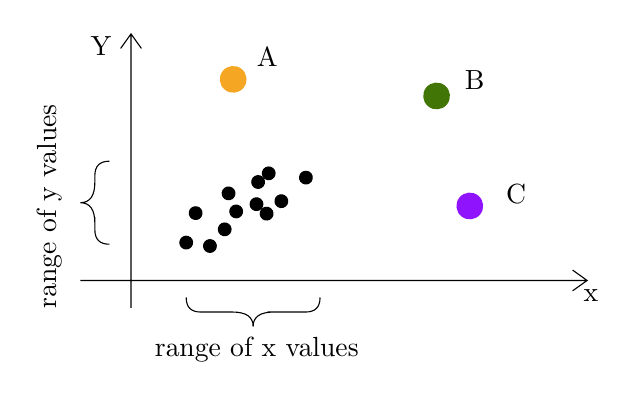
\begin{tikzpicture}[x=0.75pt,y=0.75pt,yscale=-1,xscale=1]
%uncomment if require: \path (0,195.33333206176758); %set diagram left start at 0, and has height of 195.33333206176758

%Shape: Axis 2D [id:dp9794330225749337] 
\draw  (31,131.8) -- (275.17,131.8)(55.42,13) -- (55.42,145) (268.17,126.8) -- (275.17,131.8) -- (268.17,136.8) (50.42,20) -- (55.42,13) -- (60.42,20)  ;
%Flowchart: Connector [id:dp830729222821748] 
\draw  [fill={rgb, 255:red, 0; green, 0; blue, 0 }  ,fill opacity=1 ] (114.73,86.73) .. controls (113.42,85.66) and (113.22,83.73) .. (114.29,82.42) .. controls (115.36,81.11) and (117.29,80.92) .. (118.6,81.98) .. controls (119.91,83.05) and (120.1,84.98) .. (119.04,86.29) .. controls (117.97,87.6) and (116.04,87.8) .. (114.73,86.73) -- cycle ;
%Flowchart: Connector [id:dp6451039498288915] 
\draw  [fill={rgb, 255:red, 0; green, 0; blue, 0 }  ,fill opacity=1 ] (118.81,101.97) .. controls (117.5,100.9) and (117.3,98.97) .. (118.37,97.66) .. controls (119.44,96.35) and (121.37,96.15) .. (122.68,97.22) .. controls (123.99,98.29) and (124.19,100.22) .. (123.12,101.53) .. controls (122.05,102.84) and (120.12,103.04) .. (118.81,101.97) -- cycle ;
%Flowchart: Connector [id:dp8011172696007964] 
\draw  [fill={rgb, 255:red, 0; green, 0; blue, 0 }  ,fill opacity=1 ] (91.51,117.57) .. controls (90.2,116.5) and (90,114.57) .. (91.07,113.26) .. controls (92.14,111.95) and (94.07,111.75) .. (95.38,112.82) .. controls (96.69,113.89) and (96.89,115.82) .. (95.82,117.13) .. controls (94.75,118.44) and (92.82,118.63) .. (91.51,117.57) -- cycle ;
%Flowchart: Connector [id:dp8507144087849559] 
\draw  [fill={rgb, 255:red, 0; green, 0; blue, 0 }  ,fill opacity=1 ] (98.62,109.54) .. controls (97.31,108.47) and (97.11,106.54) .. (98.18,105.23) .. controls (99.25,103.92) and (101.18,103.72) .. (102.49,104.79) .. controls (103.8,105.86) and (104,107.79) .. (102.93,109.1) .. controls (101.86,110.41) and (99.93,110.6) .. (98.62,109.54) -- cycle ;
%Flowchart: Connector [id:dp928443309589182] 
\draw  [fill={rgb, 255:red, 0; green, 0; blue, 0 }  ,fill opacity=1 ] (80.07,115.91) .. controls (78.76,114.84) and (78.57,112.91) .. (79.64,111.6) .. controls (80.71,110.29) and (82.63,110.09) .. (83.94,111.16) .. controls (85.26,112.23) and (85.45,114.16) .. (84.38,115.47) .. controls (83.31,116.78) and (81.39,116.98) .. (80.07,115.91) -- cycle ;
%Flowchart: Connector [id:dp894085737436997] 
\draw  [fill={rgb, 255:red, 0; green, 0; blue, 0 }  ,fill opacity=1 ] (119.83,82.55) .. controls (118.52,81.48) and (118.32,79.55) .. (119.39,78.24) .. controls (120.46,76.93) and (122.39,76.74) .. (123.7,77.81) .. controls (125.01,78.87) and (125.2,80.8) .. (124.13,82.11) .. controls (123.07,83.42) and (121.14,83.62) .. (119.83,82.55) -- cycle ;
%Flowchart: Connector [id:dp3127096830825926] 
\draw  [fill={rgb, 255:red, 0; green, 0; blue, 0 }  ,fill opacity=1 ] (104.15,100.91) .. controls (102.84,99.84) and (102.64,97.92) .. (103.71,96.61) .. controls (104.78,95.29) and (106.71,95.1) .. (108.02,96.17) .. controls (109.33,97.24) and (109.53,99.16) .. (108.46,100.47) .. controls (107.39,101.79) and (105.46,101.98) .. (104.15,100.91) -- cycle ;
%Flowchart: Connector [id:dp6496496287297344] 
\draw  [fill={rgb, 255:red, 0; green, 0; blue, 0 }  ,fill opacity=1 ] (113.94,97.41) .. controls (112.62,96.34) and (112.43,94.41) .. (113.5,93.1) .. controls (114.57,91.79) and (116.49,91.59) .. (117.8,92.66) .. controls (119.12,93.73) and (119.31,95.66) .. (118.24,96.97) .. controls (117.17,98.28) and (115.25,98.48) .. (113.94,97.41) -- cycle ;
%Flowchart: Connector [id:dp37437672154336576] 
\draw  [fill={rgb, 255:red, 0; green, 0; blue, 0 }  ,fill opacity=1 ] (104.04,87.25) .. controls (105.47,88.15) and (105.9,90.04) .. (105,91.47) .. controls (104.09,92.9) and (102.2,93.33) .. (100.77,92.42) .. controls (99.34,91.52) and (98.92,89.63) .. (99.82,88.2) .. controls (100.72,86.77) and (102.61,86.34) .. (104.04,87.25) -- cycle ;
%Flowchart: Connector [id:dp2062562321723702] 
\draw  [fill={rgb, 255:red, 0; green, 0; blue, 0 }  ,fill opacity=1 ] (88.19,96.75) .. controls (89.62,97.65) and (90.05,99.54) .. (89.14,100.97) .. controls (88.24,102.4) and (86.35,102.83) .. (84.92,101.92) .. controls (83.49,101.02) and (83.06,99.13) .. (83.96,97.7) .. controls (84.87,96.27) and (86.76,95.84) .. (88.19,96.75) -- cycle ;
%Flowchart: Connector [id:dp6022505758892014] 
\draw  [fill={rgb, 255:red, 0; green, 0; blue, 0 }  ,fill opacity=1 ] (141.32,79.64) .. controls (142.75,80.54) and (143.18,82.43) .. (142.27,83.86) .. controls (141.37,85.29) and (139.48,85.72) .. (138.05,84.81) .. controls (136.62,83.91) and (136.19,82.02) .. (137.09,80.59) .. controls (138,79.16) and (139.89,78.73) .. (141.32,79.64) -- cycle ;
%Flowchart: Connector [id:dp45176419201286167] 
\draw  [fill={rgb, 255:red, 0; green, 0; blue, 0 }  ,fill opacity=1 ] (129.48,91.01) .. controls (130.91,91.91) and (131.34,93.8) .. (130.44,95.23) .. controls (129.54,96.66) and (127.64,97.09) .. (126.21,96.19) .. controls (124.78,95.28) and (124.36,93.39) .. (125.26,91.96) .. controls (126.16,90.53) and (128.05,90.1) .. (129.48,91.01) -- cycle ;
%Flowchart: Connector [id:dp8281323481872875] 
\draw  [draw opacity=0][fill={rgb, 255:red, 65; green, 117; blue, 5 }  ,fill opacity=1 ] (206.71,37.91) .. controls (203.96,35.66) and (199.9,36.07) .. (197.65,38.83) .. controls (195.4,41.59) and (195.81,45.64) .. (198.57,47.89) .. controls (201.33,50.14) and (205.39,49.73) .. (207.63,46.97) .. controls (209.88,44.21) and (209.47,40.16) .. (206.71,37.91) -- cycle ;
%Flowchart: Connector [id:dp37135050597913954] 
\draw  [draw opacity=0][fill={rgb, 255:red, 144; green, 19; blue, 254 }  ,fill opacity=1 ] (222.71,90.91) .. controls (219.96,88.66) and (215.9,89.07) .. (213.65,91.83) .. controls (211.4,94.59) and (211.81,98.64) .. (214.57,100.89) .. controls (217.33,103.14) and (221.39,102.73) .. (223.63,99.97) .. controls (225.88,97.21) and (225.47,93.16) .. (222.71,90.91) -- cycle ;
%Flowchart: Connector [id:dp6196495516071849] 
\draw  [draw opacity=0][fill={rgb, 255:red, 245; green, 166; blue, 35 }  ,fill opacity=1 ] (108.71,29.91) .. controls (105.96,27.66) and (101.9,28.07) .. (99.65,30.83) .. controls (97.4,33.59) and (97.81,37.64) .. (100.57,39.89) .. controls (103.33,42.14) and (107.39,41.73) .. (109.63,38.97) .. controls (111.88,36.21) and (111.47,32.16) .. (108.71,29.91) -- cycle ;
%Shape: Brace [id:dp8715697539003557] 
\draw   (82,140) .. controls (82,144.67) and (84.33,147) .. (89,147) -- (104.25,147) .. controls (110.92,147) and (114.25,149.33) .. (114.25,154) .. controls (114.25,149.33) and (117.58,147) .. (124.25,147)(121.25,147) -- (139.5,147) .. controls (144.17,147) and (146.5,144.67) .. (146.5,140) ;
%Shape: Brace [id:dp457515066568027] 
\draw   (45,74.33) .. controls (40.33,74.33) and (38,76.66) .. (38,81.33) -- (38,84.33) .. controls (38,91) and (35.67,94.33) .. (31,94.33) .. controls (35.67,94.33) and (38,97.66) .. (38,104.33)(38,101.33) -- (38,107.33) .. controls (38,112) and (40.33,114.33) .. (45,114.33) ;

% Text Node
\draw (121,24) node   [align=left] {A};
% Text Node
\draw (221,35) node   [align=left] {B};
% Text Node
\draw (241,90) node   [align=left] {C};
% Text Node
\draw (116,165) node   [align=left] {range of x values};
% Text Node
\draw (277,139) node   [align=left] {x};
% Text Node
\draw (41,19) node   [align=left] {Y};
% Text Node
\draw (16,96) node  [rotate=-270] [align=left] {range of y values};

\end{tikzpicture}
\begin{enumerate}
	\item	To understand the difference between \textbf{outliers} and \textbf{leverage points} it is important to compare them to the mass of points and \textbf{\textit{not} the regression line}.
	\item	Outliers are points which are away from the main mass of points in the y direction (vertically).
	\begin{itemize}
		\item	When we \textit{then} add the regression line, we see this means that \textbf{outliers have a large residual}.
	\end{itemize}
	\item	Leverage points are away from the main mass of points in the x direction (horizontally).
	\begin{itemize}
		\item	There is a distinction to make between "\textit{good}" and "\textit{bad}" leverage points.
		\item	Visually, if we drew a line we can see that B is not too far out of the direction it would have whilst C is.
		\begin{itemize}
			\item	"\textit{good}" leverage points won't "damage" the model, i.e. influence the line's direction, too much.
			\item	"\textit{bad}" leverage points will. For example, C would drag the line down; it would be an \textbf{influential point}.
		\end{itemize}
		\item	To visualise, we can imagine a see-saw with C dragging down the main mass a bit:
	\end{itemize}

\tikzset{every picture/.style={line width=0.75pt}} %set default line width to 0.75pt        

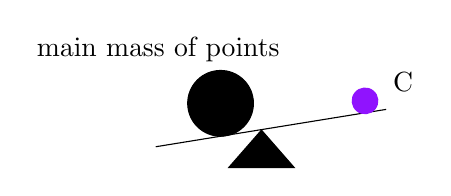
\begin{tikzpicture}[x=0.75pt,y=0.75pt,yscale=-1,xscale=1]
%uncomment if require: \path (0,195.33333206176758); %set diagram left start at 0, and has height of 195.33333206176758

%Shape: Triangle [id:dp18456202589144266] 
\draw  [fill={rgb, 255:red, 0; green, 0; blue, 0 }  ,fill opacity=1 ] (127.75,77) -- (143.5,95) -- (112,95) -- cycle ;
%Straight Lines [id:da9328191879797818] 
\draw    (76.83,85) -- (187.83,67) ;


%Flowchart: Connector [id:dp004607171227282825] 
\draw  [fill={rgb, 255:red, 0; green, 0; blue, 0 }  ,fill opacity=1 ] (98.04,76.34) .. controls (91.27,70.82) and (90.26,60.85) .. (95.78,54.08) .. controls (101.3,47.31) and (111.27,46.29) .. (118.04,51.81) .. controls (124.82,57.34) and (125.83,67.3) .. (120.31,74.08) .. controls (114.79,80.85) and (104.82,81.87) .. (98.04,76.34) -- cycle ;
%Flowchart: Connector [id:dp3540795933589729] 
\draw  [draw opacity=0][fill={rgb, 255:red, 144; green, 19; blue, 254 }  ,fill opacity=1 ] (181.71,57.91) .. controls (178.96,55.66) and (174.9,56.07) .. (172.65,58.83) .. controls (170.4,61.59) and (170.81,65.64) .. (173.57,67.89) .. controls (176.33,70.14) and (180.39,69.73) .. (182.63,66.97) .. controls (184.88,64.21) and (184.47,60.16) .. (181.71,57.91) -- cycle ;

% Text Node
\draw (78,38) node   [align=left] {main mass of points};
% Text Node
\draw (196,54) node   [align=left] {C};


\end{tikzpicture}

\end{enumerate}
\end{YTB_SUMM}

\begin{YTB_SUMM}{\href{https://www.youtube.com/watch?v=31xA3hsxW6k}{Phil Chan: Influential points - Cook's distance, DFFITS, DFBETAS}}
\begin{enumerate}
	\item	Influential points affect both \textbf{output} and \textbf{conclusions} important ways.
	\item	The video covers 3 measures:
	\begin{itemize}
		\item	Cook's distance and DFFIT measure the \textbf{overall} change in paremeters when \textbf{each point in turn} is deleted.
		\item	DFBETA breaks it down to the individual change per parameter.
	\end{itemize}
	\item	More generally, the level of inflation is proportional to the scaled residual (\textbf{outlyingness}) and it's \textbf{degree of leverage} in a multiplicative way.
	\begin{equation*}
		\text{influence on parameters} = f(\text{leverage}) \times g(\text{outlyingness})
	\end{equation*}
	\item	Finally, the important lesson is \textbf{don't just delete terms}, \textit{reason it}.
	\begin{itemize}
		\item	The example has a model of prestige in function of income and education with a minister as an outlier. 
		\item	If we just deleted the minister without thinking, we'd of missed an important insight into the model.
	\end{itemize}
\end{enumerate}
\end{YTB_SUMM}

\begin{YTB_SUMM}{\href{https://www.youtube.com/watch?v=xc_X9GFVuVU}{jbstatistics: Leverage and Influential Points in Simple Linear Regression}}
I didn't watch the whole video (because time) but it breaks down the formula for leverage very well towards the end.
\begin{enumerate}
	\item	The formula for leverage is $h_{ii} = \frac{1}{n} + \frac{(x_{i} - \bar{x})^{2}}{\sum_{j = 1}^{n}(x_{j} - \bar{x})^{2}}$.
	\begin{itemize}
		\item	Thus if the point $x_{i}$ is far from the average, the denominator wll be large causing the leverage to be high and vice-versa.
	\end{itemize}
\end{enumerate}
\end{YTB_SUMM}

\begin{YTB_SUMM}{\href{https://www.youtube.com/watch?v=0SBIXgPVex8}{Ben Lambert: Variance Inflation Factors: testing for multicollinearity}}
\begin{enumerate}
	\item	The idea of the VIF is that we want to evaluate relationships between variables.
	\begin{itemize}
		\item	Usually, we would use a \textit{correlation matrix} to compare the correlation of 2 variables and see if there's any relationship between them;
		\item	Usually, we would use a \textit{scatterplot} to compare one variable to all of the others and see if there's any relationships between them;
		\item	The "\textit{problem}" with both of these is that they're \textbf{\textit{bivariate} methods only};
		\item	Therefore, we want to generalize these and want to \textbf{explain one variable} as a \textbf{combination}, \textit{or \textbf{linear combination}}, \textbf{of the other variables}.
	\end{itemize}
	\item	That being the idea for the \textbf{VIF}, we regress one of the explanatory variable $x_{j}$ as a fonction of all the others.
	\item	We then find the $R^{2}$ of this new regression denoted $R^{2}_{(j)}$.
	\item	We then repeat this for all of the explanatory variables in the regression.
	\begin{itemize}
		\item	A \textbf{high value} of $R^{2}_{(j)}$ means it's likely there is \textbf{multicolinearity} with the \textbf{\textit{linear} combination} of the other variables;
		\item	However, $R^{2}$ is hard to compare so we want to \textbf{\textit{inflate} the differences} between the different values of $R^{2}_{(j)}$.
	\end{itemize}
	\item	Therefore, we define $\text{VIF}_{j} = \frac{1}{1 - R^{2}_{(j)}}$.
	\begin{itemize}
		\item	If $R^{2}_{(j)}$ is large, then so will the $\text{VIF}_{j}$; 
		\item	As such, we want to minimise the $\text{VIF}_{j}$.
	\end{itemize}
\end{enumerate}
\end{YTB_SUMM}

\begin{YTB_SUMM}{\href{https://www.youtube.com/watch?v=fSytzGwwBVw}{StatQuest: Machine Learning Fundamentals: Cross Validation}}
This video enables us to see the direct link between the holdout sample method, k-fold CV, and LOOCV. Also, visualise the four 25\% blocks for the cross-validation.
\begin{enumerate}
	\item	If we used all the data for training, then there'd be no way to test the algorithm.
	\item	A \textit{slightly} better idea would be to use 75\% of the data for training and 25\% for testing.
	\begin{itemize}
		\item	The downside is that the 25\% we choose is arbitrary, why one block and not another?
	\end{itemize}
	\item	An \textit{even better} idea is thus to adjust the model with 3 blocks and test one the 4th one 4 times. 
	\begin{itemize}
		\item	This is \textbf{$k$-fold cross validation} with $k = 4$.
	\end{itemize}
	\item	If we set $k = n$, we adjust the model and test the data for every observation. This is $n$-fold cross-validation, or rather \textbf{Leave One Out Cross-Validation \textit{(LOOCV)}}.
	\item	A \textbf{tuning parameter} is a parameter that's not estimated but guessed (like lambda in Ridge/Lasso regression). We can therefore use $k$-fold cross validation to help find the best value for it.
\end{enumerate}
\end{YTB_SUMM}

\begin{YTB_SUMM}{\href{https://www.youtube.com/watch?v=Q81RR3yKn30&list=PLblh5JKOoLUICTaGLRoHQDuF_7q2GfuJF}{StatQuest: Regularization Part 1: Ridge Regression}}
\begin{enumerate}
	\item	J'ai écouté ce vidéo et le prochain pendant la session et ils sont incroyable pour bien expliquer. Cependant, pas le temps en ce moment pour les regarder encore.
\end{enumerate}
\end{YTB_SUMM}

\begin{YTB_SUMM}{\href{https://www.youtube.com/watch?v=NGf0voTMlcs&list=PLblh5JKOoLUICTaGLRoHQDuF_7q2GfuJF}{StatQuest: Regularization Part 2: Lasso Regression}}
\begin{enumerate}
	\item	J'ai écouté ce vidéo et le dernier pendant la session et ils sont incroyable pour bien expliquer. Cependant, pas le temps en ce moment pour les regarder encore.
\end{enumerate}
\end{YTB_SUMM}

\section{Prévisions et interprétations}

\subsection{Résumés des chapitres}

\begin{CHPT_SUMM}[label = {PREV-PREDICTIONS}]{\addcontentsline{toc}{subsubsection}{9. Linear Regression:  Predictions}9. Linear Regression:  Predictions}
\noindent
\begin{tabular}{|l|l|}
\hline
\rowcolor[HTML]{21650A} 
\multicolumn{1}{|c|}{\cellcolor[HTML]{21650A}{\color[HTML]{FFFFFF} \textbf{Parameter Risk}}}                                                        & \multicolumn{1}{c|}{\cellcolor[HTML]{21650A}{\color[HTML]{FFFFFF} \textbf{Process Risk}}}                                                               \\ \hline
\rowcolor[HTML]{B8F0A5} 
intervalle de confiance                                                                                                                             & intervalle de prévision                                                                                                                                 \\ \hline
\rowcolor[HTML]{B8F0A5} 
pour la valeur moyenne                                                                                                                              & pour la valeur prédite                                                                                                                                  \\ \hline
\rowcolor[HTML]{B8F0A5} 
E$[Y^* | x^*] = \beta_0 + \beta_1 x^*$                                                                                                              & $Y^* = \beta_0 + \beta_1 x^*$                                                                                                             \\ \hline
\rowcolor[HTML]{B8F0A5} 
{\color[HTML]{333333} $\hat{y}^* \pm t_{1 - \frac{\alpha}{2}, n - 2} s \sqrt{\frac{1}{n} + \frac{(x^* - \bar{x})^2}{\sum_{i = 1}^{n}(x_i - \bar{x})^2}}$} & {\color[HTML]{333333} $\hat{y}^* \pm t_{1 - \frac{\alpha}{2}, n - 2} s \sqrt{1 + \frac{1}{n} + \frac{(x^* - \bar{x})^2}{\sum_{i = 1}^{n}(x_i - \bar{x})^2}}$} \\ \hline
\end{tabular}

En régression linéaire multiple, $\widehat{\text{Var}}(y^{*}) = s^{2}(1 + \matr{(x^{*})^{\top}(X^{\top}X)^{-1}x^{*}})$
\textbf{Note sur les exercices:} 
\begin{enumerate}
	\item	Les questions d'examen semble être plus axée sur utiliser les relations pour arriver à un intervalle de prévision;
	\item	Ne semble pas que le multivarié serait sur l'examen donc difficile de juger si apprendre ses formules vaut la peine.
\end{enumerate}
\end{CHPT_SUMM}

\begin{CHPT_SUMM}[label = {PREV-INTERP}]{\addcontentsline{toc}{subsubsection}{10. Interpreting Regression Results}10. Interpreting Regression Results}
\begin{enumerate}
	\item	Statistical significance.
	\begin{itemize}
		\item	Statistical significance $\neq$ practical significance. L'estimation du paramètre pourrait être trops faible pour avoir un vrai impact en dollars et sous;
		\item	$s_{b_{j}} = \frac{s}{\sqrt{n - 1}}\frac{\sqrt{VIF_{j}}}{s_{x_{j}}}$ est donc influencé par 4 facteurs, une augmentation de la signifiance (décroissance de $s_{b_{j}}$) peut être en raison de:
		\begin{enumerate}
			\item	Une baisse de $s$ qui peut être réduit en mesurant plus précisément $y$;
			\item	Une baisse du $VIF_{j}$ qui être réduit en utilisant des variables explicatives moins colinéaires;
			\item	Une augmentation de $\sqrt{n - 1}$ en ayant plus d'observations;
			\item	Une augmentation de $s_{x_{j}}$ avec des variables plus écartées.
		\end{enumerate}
	\end{itemize}
	\item	Utilités des modèles de régression.
	\item[]	Déterminer si le prix d'une maison est raisonnable avec un modèle de régression linéaire simple.
	\item	Sélection de variables.
	\item[]	\textbf{Positifs} du overfitting:
	\begin{itemize}
		\item	Prévisions seront sans biais. Exclure une variable pertinente peut mener à un biais.
	\end{itemize}
	\item[]	\textbf{Négatifs} du overfitting:
	\begin{itemize}
		\item	Les modèles plus simple sont plus faciles à interpréter;
		\item	Les modèles plus simples vont mieux performer avec des données externes;
		\item	Les variables inutiles peuvent mener à de la colinéarité;
	\end{itemize}
	\item	Data collection
	\begin{itemize}
		\item	\textbf{Sampling frame error}: mauvaise population est utilisée pour choisir un échantillon. (pour exemple, ceux qui achète des bonds pensent déjà vivre plus longtemps donc ce n'est pas un échantillon représentatif de la population);
		\item	Les variables explicatives pourrait être \textbf{censurées}. Des données censurées de façon significative peut mener à un biais dans l'estimation des coefficients;
		\item	Les variables explicatives pourrait être \textbf{tronquées}. Ceci est un problème plus sévère que des données censurées puisqu'elles ne sont pas observées du tout;
		\item	L'\textbf{exclusion} de variables explicatives peut mener à un \textbf{biais};
		\item[]	De plus, ceci peut mener à l'inclusion de variables endogènes (dépendantes sur d'autres variables) comme l'exemple de séries chronos.
		\item	Il peut avoir un problème de \textbf{données manquantes}.
	\end{itemize}
\end{enumerate}
\end{CHPT_SUMM}

\section{Modèles linéaires généralisés}

\subsection{Résumés des chapitres}

\begin{CHPT_SUMM}[label = {GLM-BASICS}]{\addcontentsline{toc}{subsubsection}{11. Basics}11. Basics}
\begin{enumerate}
	\item	Famille exponentielle linéaire
	\begin{itemize}
		\item	Paramètres de dispersion et d'\textbf{échelle};
		\item	Savoir Tweedie;
	\end{itemize}
	\item	Fonction de lien
	\begin{itemize}
		\item	Modéliser \textit{une fonction} de la moyenne - prédicteur linéaire;
		\item	L'estimation du GLM est sans biais lorsque la fonction de lien canonique est utilisée;
	\end{itemize}
	\item	Estimation
	\begin{itemize}
		\item	Matrice d'information Fisher;
		\item	Les dérivées partielles sont les \textit{scores};
	\end{itemize}
	\item	Sur-dispersion
	\begin{itemize}
		\item	Estimation du paramètre de dispersion via la statistique du khi-carré de Pearson;
	\end{itemize}
\end{enumerate}
\textbf{Note sur les exercices:} 
\begin{enumerate}
	\item	Trouver des fonctions d'une distribution t.q. $\text{Var}(Y)$, $\text{V}(\mu)$, $b(\theta)$, etc.;
	\item	Déterminer si une distribution fait partie de la famille exponentielle (domaine, etc.);
	\item	\textbf{Trouver la prévision de l'espérance ou la variance} à partir de données;
	\item[]	Vraiment beaucoup de ce dernier type pour MAS-I / S et c'est \textbf{vraiment facile}, donc probable que ce serait dans SRM;
	\item	Questions à choix multiple.
\end{enumerate}
\end{CHPT_SUMM}

\begin{CHPT_SUMM}[label = {GLM-CAT}]{\addcontentsline{toc}{subsubsection}{12. Categorical Response}12. Categorical Response}
\begin{enumerate}
	\item	Binomial (binary) response
	\begin{itemize}
		\item	$\eta$ est le \textbf{systematic component};
		\item	Dans un \textbf{logistic model}, $\eta = \ln\left( \frac{\pi}{1 - \pi} \right)$;
		\item	Idée du \textit{treshold interpretation} avec $y^{*} = \eta + \varepsilon$ que l'on isole;
	\end{itemize}
	\item[]	On devrait s'attendre à peu, ou aucune, questions sur ces 2 sujets (réponse ordinale et nominale) et l'auteur suggère qu'on \textbf{peut même les sauter en entier si on est pressé}.
	\item	Nominal response	
	\begin{itemize}
		\item	Généralisation du binary response avec plus de catégories, $c > 2$;
		\item	Peut calculer le \textbf{relative odds} de la catégorie $j$ à la catégorie de base $c$.
	\end{itemize}
	\item	Ordinal response
	\begin{itemize}
		\item	Les catégories ont un ordre;
		\item	Idée du odds ratio qui est maintenant cumulatif et peut soit avoir un coefficient différent pour chaque catégorie ou pas (sauf l'intercepte qui sera toujours différent).
	\end{itemize}
\end{enumerate}
\textbf{Note sur les exercices:} Personnellement j'en ai arraché pas mal dans ce chapitre avec la réponse nominale / ordinale. Ceci dit, peu probable que ce sera dans l'exam donc c'est ça.
\begin{enumerate}
	\item	Réponse binaire généralement:
	\begin{itemize}
		\item	Exercices qu'il faut trouver le odds ratio (5, 9 à 12, 17);
		\item	Exercices qu'il faut trouver une prob / une différence de probs (4, 6 à 8, 13 à 16).
	\end{itemize}
	\item	Réponse nominale généralement:
	\begin{itemize}
		\item	Exercices qu'il faut trouver le odds ratio (19 à 20);
		\item	Exercices qu'il faut trouver une prob / une différence de probs (21 à 24).
	\end{itemize}
	\item	Réponse ordinale généralement:
	\begin{itemize}
		\item	Exercices qu'il faut trouver le odds ratio / cumulative odds ratio / relative odds ratio (26, 27, 32);
		\item	Exercices qu'il faut trouver une prob / une différence de probs (25, 27, 29 à 31, 33 à 35);
		\item	J'ai éprouvé beaucoup de difficulté à bien comprendre comment isoler la probabilité et/ou le odds ratio pour le lien logit; mais, peu probable que ce soit dans l'examen donc à votre guise.
	\end{itemize}
\end{enumerate}
\end{CHPT_SUMM}

\begin{CHPT_SUMM}[label = {GLM-COUNT}]{\addcontentsline{toc}{subsubsection}{13. Count Response}13. Count Response}
\begin{enumerate}
	\item	Poisson response
	\item	Sur-dispersion et modèles avec binomiale négative;
	\item[]	Noter la formule pour estimer le paramètre de dispersion et le lien avec celle de chapitre 11.
	\item	Other count models
	\item[]	Noter que les formules pour la \textcolor{darkpastelpurple}{l'espérance} et la \textcolor{teal}{variance} sont du même format pour les trois.
	\begin{enumerate}
		\item	\textbf{Zero-inflated} models;
		\begin{align*}
			\Pr(Y = j) &= 
			\begin{cases}
				\pi	+ (1 - \pi) h(0)	&	j = 0	\\
				(1 - \pi) h(j)		&	j > 0	\\
			\end{cases}	\\
			\text{E}[Y_{i}]		&=	\textcolor{darkpastelpurple}{(1 - \pi_{i}) \mu_{i}}	\\
			\text{Var}(Y_{i})	&=	\textcolor{darkpastelpurple}{(1 - \pi_{i}) \mu_{i}} + \textcolor{teal}{\pi_{i} (1 - \pi_{i})} \textcolor{cyan}{\mu_{i}^{2}}
		\end{align*}
		\item	\textbf{Hurdle} models: Rationale is that the response is the result of a two-step process:
		\begin{itemize}
			\item	The decision to make the count greater than 0 (the hurdle);
			\item	Determining the non-zero count.
		\end{itemize}
		\begin{align*}
			\Pr(Y = j) &= 
			\begin{cases}
				\pi	&	j = 0	\\
				k h(j)	&	j > 0	\\
			\end{cases}	\\
			\text{E}[Y_{i}]		&=	\textcolor{darkpastelpurple}{k \mu_{i}}	\\
			\text{Var}(Y_{i})	&=	\textcolor{darkpastelpurple}{k \mu_{i}} + \textcolor{teal}{k (1 - k)} \textcolor{cyan}{\mu_{i}^{2}} \\
			&\text{De plus, on trouve: } \\
			k < 1 &\Rightarrow 1 - k > 0 \therefore \text{Var} > \text{E}	\\
			k > 1 &\Rightarrow 1 - k < 0 \therefore \text{Var} < \text{E}	
		\end{align*}
		où $k = \frac{1 - \pi}{1 - h(0)}$
		\item	\textbf{Heterogeneity} models;
		\item[] Lorsque $\{Y_{i} | \alpha_{i} \} \sim \text{Poisson}$, on a:
		\begin{align*}
			\text{E}[Y_{i}]		&=	\textcolor{darkpastelpurple}{\mu_{i}}	\\
			\text{Var}(Y_{i})	&=	\textcolor{darkpastelpurple}{\mu_{i}} + \textcolor{teal}{\text{Var}(\text{e}^{\alpha_{i}})} \textcolor{cyan}{\mu_{i}^{2}}
		\end{align*}
		\item	\textbf{Latent} models;
	\end{enumerate}
\end{enumerate}
\textbf{Note sur les exercices:} 
\begin{enumerate}
	\item	Poisson
	\begin{itemize}
		\item	Une bonne question un peu plus tricky serait une comme le numéro 5;
		\item	De plus, le numéro 9 est une bonne pratique pour question que je crois pourrait être dans l'examen;
		\item	Aussi, des questions classiques comme trouver la variance/espérance/offset/... ce à quoi les questions d'examen semble plus se rapprocher.
	\end{itemize}
	\item	Autres
	\begin{itemize}
		\item	Ça revient pas mal toujours à soit trouver une prob (hurdle et poisson gonflée à zéro) ou trouver la variance / espérance (tous);
		\item	Pour apprendre les formules des variances / espérance, ça devient facile en voyant la pattern commune aux trois!;
		\item	Dans tous les cas, il n'avait pas de questions d'exam sur ces 4 modèles et la feuille de formule de Coaching n'inclut pas les formules pour.
	\end{itemize}
\end{enumerate}
\end{CHPT_SUMM}

\begin{CHPT_SUMM}[label = {GLM-MEZ-FIT}]{\addcontentsline{toc}{subsubsection}{14. Measures of Fit}14. Measures of Fit}
\textbf{Note importante}: Lorsqu'on test si un modèle est une simplification adéquate d'un autre, on teste (pour exemple):
\begin{align*}
	\mathcal{H}_{0}&: \beta_{1} = \beta_{2} = 0	&
	\mathcal{H}_{1}&: \beta_{1} \neq 0 \cup \beta_{2} \neq 0
\end{align*}
Mais ceci \textit{n'est \textbf{pas} un test bilatéral}! En réalité, on test:
\begin{align*}
	\mathcal{H}_{0}&: p = 0	&
	\mathcal{H}_{1}&: p > 0 
\end{align*}
Ce qui est un test unilatéral et donc on veut que la statistique du TRV soit $> \chi^{2}_{q, 1 - \alpha}$. Le seuil n'est pas divisé par deux.
\begin{enumerate}
	\item	\textbf{Pearson chi-square}: Pour évaluer la qualité d'ajustement d'un modèle.
	\begin{itemize}
		\item	Si les données sont groupées on utilise la première définition avec le $X^{2} = \sum_{i = 1}^{n}\frac{(n_{i} - n \hat{p}_{i})^{2}}{n \hat{p}_{i}}$;
		\item	Si les donnés sont par observations (indépendantes) on utilise $X^{2} = \sum_{i = 1}^{n}\frac{(y_{i} - \hat{\mu}_{i})^{2}}{\phi \text{V}(\hat{\mu}_{i})}$.
	\end{itemize}
	\item	\textbf{Likelihood Ratio Test \textit{(LRT)}}
	\begin{itemize}
		\item	On peut voir le test du rapport de vraisemblance comme l'équivalent du test $F$ pour les GLMs;
		\item[]	On évalue si un modèle, ou un ensemble de ses paramètres, est significatif	s;
		\item	Statistique: $LRT = -2(\tilde{\ell} - \hat{\ell}) \approx	\chi_{q}^{2}$;
		\item[]	$q$ est le nombre de contraintes (paramètres à retirer)
		\item[]	$\hat{\ell}$ est la log-vraisemblance du modèle sans contraintes \textbf{(complet)};
		\item[]	$\tilde{\ell}$ est la log-vraisemblance du modèle avec contraintes \textbf{(réduit)};
	\end{itemize}
	\item	\textbf{Deviance}: Pour évaluer la qualité d'ajustement d'un modèle;
	\item[]	$D = 2 \phi \left( \ell(\bm{b}_{\text{saturé}}) - \ell(\bm{b}) \right) \approx \chi^{2}_{n - p'}$.
	\begin{itemize}
		\item	On peut voir la déviance comme la \textit{déviance}, ou \textbf{l'écart}, entre les observations et les prévisions. 
		\item[]	Si ceci semble familier, c'est puisque c'est l'interprétation du SSE en régression linéaire simple;
		\item[]	Donc, \textit{(\textbf{je} pose que)} on peut voir la déviance comme étant l'équivalent aux GLMs \textbf{de la famille exponentielle} du SSE;
		\item	La loi normale exemplifie ceci avec une déviance = SSE;
		\item	Par la suite, les déviances des distributions Bernoulli et Poisson deviennent logique avec ceci en tête:
		\begin{align*}
			D	&=	-2 \left( \underset{y_{i} = 1}{\sum} \ln(\hat{y}_{i}) \underset{y_{i} = 0}{\sum} \ln(1 - \hat{y}_{i}) \right)	\\
			D	&=	2 \sum_{i = 1}^{n} \left[ y_{i} \ln \left( \frac{y_{i}}{\hat{y}_{i}} \right) - (y_{i} - \hat{y}_{i}) \right]
		\end{align*}
		\item[]	De plus, lorsqu'un lien log et que le coefficient $\beta_{0}$ sont utilisés, et que la somme des résidus est nulle ($\sum (y_{i} - \hat{y}_{i}) = 0$) on obtient $\ln(1) = 0$. Ce faisant, la deuxième partie de la formule de la déviance pour la Poisson peut être omise;
		\item	Plus formellement, le \textbf{modèle saturé} est le modèle avec le \textit{meilleur ajustement possible}. C'est-à-dire qu'il y a un paramètre par observation;
		\item	La \textbf{scaled deviance} est la statistique comparant le modèle saturé au modèle proposé;
		\item	La \textbf{déviance} est ré-obtenue en multipliant le paramètre d'échelle $\phi$ avec la scaled deviance;
	\item On généraliser également le TRV, $LRT = -2(\tilde{\ell} - \hat{\ell}) = (\tilde{D} - \hat{D}) \approx	\chi_{q}^{2}$;
		\begin{itemize}
			\item	Donc, avec la déviance on appel le modèle complet / sans contraintes le \textit{modèle saturé} puisqu'on compare notre modèle à celui de base au lieu de comparer 2 modèles;
			\item	Pareillement, lorsqu'on récrit le TRV avec la déviance on retourne à la notation réduit vs complet (avec vs sans contraintes);
			\item	Finalement, on note que la log-vraisemblance du modèle complet (saturé) devrait être supérieure à celle du modèle réduite;
		\end{itemize}
	\end{itemize}
	\item	Penalized loglikelihood tests
	\begin{align*}
		AIC &= -2 \ell(\bm{\hat{\beta}}) + 2 p'	&
		BIC &= -2 \ell(\bm{\hat{\beta}}) + \ln (n) p'
	\end{align*}
	\begin{itemize}
		\item	On rappel que $\bm{\hat{\beta}}$ est le vecteur des $p' = p + 1$ coefficients et donc la pénalité est de $p'$;
		\item	Cependant, s'il a également un paramètre de dispersion $\phi$ à estimer alors la pénalité est $p + 2$;
	\end{itemize}
	\item	Max-scaled $R^{2}$ and pseudo-$R^{2}$
	\begin{align*}
		R^{2}_{ms}	&=	\frac{1 - \e{2\left(\ell_{0} - \ell(\bm{\hat{\beta}})\right)/n}}{1 - \e{2 \ell_{0}/n}}	&
		R^{2}_{pse.}	&=	\frac{\ell_{0} - \ell(\bm{\hat{\beta}})}{\ell_{0} - \hat{\ell}}
	\end{align*}
	\begin{itemize}
		\item	Le \og \textit{problème} \fg{} avec le max-scaled $R^{2}_{ms}$ est qu'il sera uniquement 1 pour un modèle parfait puisqu'avec un modèle parfait, $\ell(\bm{\hat{\beta}}) = 0$ et donc le ratio est de 1;
		\item	Dans le cas de régression linéaire simple, le pseudo $R^{2}_{pse.}$ se réduit à uniquement $R^{2}$;
	\end{itemize}
	\item	Résidus
	\begin{itemize}
		\item	Utilités:
		\begin{itemize}
			\item	Identifier les covariantes et/ou les pattern;
			\item	Identifier les outliers;
			\item	Illustrer l'hétéroscédasticité / tendances temporelles;
			\item	Individuellement illustrer l'impact d'une variable explicative sur le modèle;
		\end{itemize}
		\item	\textbf{Pearson} 
		\item	\textbf{Deviance} 
		\item	\textit{Anscombe} 
	\end{itemize}
\end{enumerate}
\textbf{Note sur les exercices:} 
\begin{enumerate}
	\item	\textbf{Pearson chi-square} (3 -> 1 past/sample exam questions)
	\begin{itemize}
		\item	Bien distinguer le cas de données groupées du cas de données individuelles;
		\item	Noter que la fonction de variance est celle pour la famille exponentielle dans la 2e définition;
	\end{itemize}
	\item	\textbf{LRT et deviance} (12 -> 5 past/sample exam questions)
	\begin{itemize}
		\item	Beaucoup d'anciennes questions d'examens donc à savoir;
		\item	Très utile de connaître les formules de la déviance pour les 3 distributions ainsi que la simplification pour la Poisson sinon faut recalculer à chaque fois;
		\item	Bien saisir les seuils et les tests d'hypothèse pour la khi-carré;
	\end{itemize}
	\item	\textbf{AIC} et \textbf{BIC} (12 -> 6 past exam questions)
	\begin{itemize}
		\item	Ces questions sont plutôt difficiles et ont apparu systématiquement dans les examens de la S/MAS-I. Ce faisant, il me semble logique qu'elles apparaissent dans SRM;
		\item	Je conseille de noter ce type d'exercices comme des exercices à pratiquer puisqu'il faut vraiment connaître les liens entre le TRV/AIC/BIC comme sa poche;
		\item	Également, faut comprendre l'impact et le raisonnement sous-jacente à la pénalité des paramètres;
	\end{itemize}
	\item	Max-scaled $R^{2}$ and pseudo-$R^{2}$: savoir les formules. (4)
	\item	Résidus: savoir les formules. (4)
\end{enumerate}
\end{CHPT_SUMM}

\subsection{Notes sur les vidéos YouTube}

\begin{YTB_SUMM}{\href{https://www.youtube.com/watch?v=yIYKR4sgzI8}{StatQuest: Logistic Regression}}
\begin{enumerate}
	\item	Logistic regression predicts whether something is T/F, instead of predicting something continuous like size.
	\item	Instead of fitting a line, we fit a "s" shaped logistic function.
	\begin{itemize}
		\item	The curve therefore goes from 0 to 1 and \textbf{predicts a probability} that a mouse is obese based on its weight;
		\item	If we weighed a heavy mouse, a high probability it's obese; if weighed a light mouse high probability it's not obese.
	\end{itemize}
	\item	Logistic regression usually \textbf{used for classification}.
	\item[]	For example, if the probability that a mouse is obese is > 50\% then we'll \textbf{classify} it as obese.
	\item	We can make simple models. 
	\item[]	For example, Obesity in function of Weight.
	\item	We can have continuous, categorical, etc. types of variables.
	\begin{itemize}
		\item	We test if a variable's effect on the prediction is significantly different from 0 but can't directly compare 2 models like in linear regression (Wald's test).
	\end{itemize}
	\item	Logistic regression \textbf{fits the line differently} than linear regression
	\begin{itemize}
		\item	In linear regression, we fit with least squares where the sum of the residuals is minimised;
		\item	In logistic regression we don't have the same concept of a "residual" and thereby can't use least squares nor calculate $R^{2}$ but uses maximum likelihood instead;
		\item	Calculate likelihood of observing each data point and multiply them together;
		\item	Then shift the line and repeat until the curve with the maximum likelihood is found.
	\end{itemize}
\end{enumerate}
\end{YTB_SUMM}


\begin{YTB_SUMM}{\href{https://www.youtube.com/watch?v=pYxNSUDSFH4&feature=youtu.be}{StatQuest: Probability vs Likelihood}}
\begin{enumerate}
	\item	Probability is what we're used to: Prob(mouse weighs 34 grams | mean = 34, standard deviation = 2.5) = \textbf{Pr(data | distribution)}.
	\item[]	We find the most likely observations given some parameters for the curve. 
	\item[]	It's the area under a fixed distribution.
	\item	Likelihood: L(mean = 34, standard deviation = 2.5 | mouse weighs 34 grams) = \textbf{L(distribution | data)}.
	\item[]	We find the most likely curve given some oboservation(s).
	\item[]	Likelihoods are the y-axis value for fixed data points with distributions which can be moved.
\end{enumerate}
\end{YTB_SUMM}

\begin{YTB_SUMM}{\href{https://www.youtube.com/watch?v=XepXtl9YKwc&feature=youtu.be}{StatQuest: Maximum Likelihood, clearly explained!!!}}
\begin{enumerate}
	\item	Depending on where we plot the normal density curve, the probability of observing our data points can go up or down.
	\item	We plot the curve around the mean which we then shift around.
	\item	We shift the location of the mean, around which the curve is centered, until we find the location that maximises the \textbf{likelihood} of observing the weights we measured.
	\item[]	This is the \textbf{maximum likelihood estimate for the mean} (of the distribution, not data but for a normal those are equal).	
	\item	The MLE for the standard deviation is the same procedure.
\end{enumerate}

\tikzset{every picture/.style={line width=0.75pt}} %set default line width to 0.75pt        

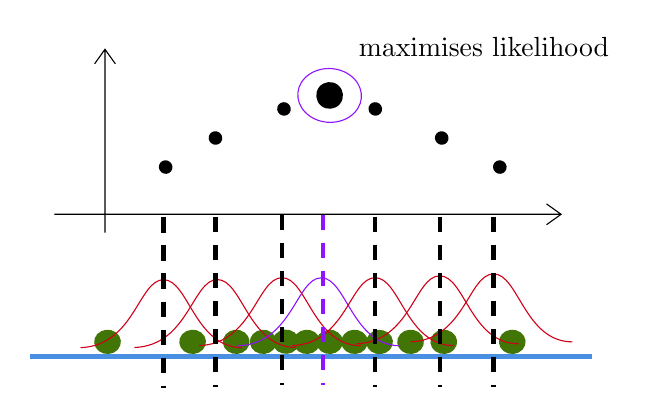
\begin{tikzpicture}[x=0.75pt,y=0.75pt,yscale=-1,xscale=1]
%uncomment if require: \path (0,195.33333206176758); %set diagram left start at 0, and has height of 195.33333206176758

%Flowchart: Connector [id:dp16864482457380792] 
\draw  [draw opacity=0][fill={rgb, 255:red, 65; green, 117; blue, 5 }  ,fill opacity=1 ] (75.71,159.09) .. controls (72.96,157.04) and (68.9,157.42) .. (66.65,159.93) .. controls (64.4,162.44) and (64.81,166.13) .. (67.57,168.17) .. controls (70.33,170.21) and (74.39,169.84) .. (76.63,167.33) .. controls (78.88,164.82) and (78.47,161.13) .. (75.71,159.09) -- cycle ;
%Flowchart: Connector [id:dp9802591055616827] 
\draw  [draw opacity=0][fill={rgb, 255:red, 65; green, 117; blue, 5 }  ,fill opacity=1 ] (137.71,159.09) .. controls (134.96,157.04) and (130.9,157.42) .. (128.65,159.93) .. controls (126.4,162.44) and (126.81,166.13) .. (129.57,168.17) .. controls (132.33,170.21) and (136.39,169.84) .. (138.63,167.33) .. controls (140.88,164.82) and (140.47,161.13) .. (137.71,159.09) -- cycle ;
%Flowchart: Connector [id:dp05225203779633203] 
\draw  [draw opacity=0][fill={rgb, 255:red, 65; green, 117; blue, 5 }  ,fill opacity=1 ] (116.71,159.09) .. controls (113.96,157.04) and (109.9,157.42) .. (107.65,159.93) .. controls (105.4,162.44) and (105.81,166.13) .. (108.57,168.17) .. controls (111.33,170.21) and (115.39,169.84) .. (117.63,167.33) .. controls (119.88,164.82) and (119.47,161.13) .. (116.71,159.09) -- cycle ;
%Flowchart: Connector [id:dp2760284772295425] 
\draw  [draw opacity=0][fill={rgb, 255:red, 65; green, 117; blue, 5 }  ,fill opacity=1 ] (171.71,159.09) .. controls (168.96,157.04) and (164.9,157.42) .. (162.65,159.93) .. controls (160.4,162.44) and (160.81,166.13) .. (163.57,168.17) .. controls (166.33,170.21) and (170.39,169.84) .. (172.63,167.33) .. controls (174.88,164.82) and (174.47,161.13) .. (171.71,159.09) -- cycle ;
%Flowchart: Connector [id:dp6624437432554011] 
\draw  [draw opacity=0][fill={rgb, 255:red, 65; green, 117; blue, 5 }  ,fill opacity=1 ] (150.71,159.09) .. controls (147.96,157.04) and (143.9,157.42) .. (141.65,159.93) .. controls (139.4,162.44) and (139.81,166.13) .. (142.57,168.17) .. controls (145.33,170.21) and (149.39,169.84) .. (151.63,167.33) .. controls (153.88,164.82) and (153.47,161.13) .. (150.71,159.09) -- cycle ;
%Flowchart: Connector [id:dp03313254158829326] 
\draw  [draw opacity=0][fill={rgb, 255:red, 65; green, 117; blue, 5 }  ,fill opacity=1 ] (194.71,159.09) .. controls (191.96,157.04) and (187.9,157.42) .. (185.65,159.93) .. controls (183.4,162.44) and (183.81,166.13) .. (186.57,168.17) .. controls (189.33,170.21) and (193.39,169.84) .. (195.63,167.33) .. controls (197.88,164.82) and (197.47,161.13) .. (194.71,159.09) -- cycle ;
%Flowchart: Connector [id:dp8229616225061853] 
\draw  [draw opacity=0][fill={rgb, 255:red, 65; green, 117; blue, 5 }  ,fill opacity=1 ] (182.71,159.09) .. controls (179.96,157.04) and (175.9,157.42) .. (173.65,159.93) .. controls (171.4,162.44) and (171.81,166.13) .. (174.57,168.17) .. controls (177.33,170.21) and (181.39,169.84) .. (183.63,167.33) .. controls (185.88,164.82) and (185.47,161.13) .. (182.71,159.09) -- cycle ;
%Flowchart: Connector [id:dp7001184718325861] 
\draw  [draw opacity=0][fill={rgb, 255:red, 65; green, 117; blue, 5 }  ,fill opacity=1 ] (221.71,159.09) .. controls (218.96,157.04) and (214.9,157.42) .. (212.65,159.93) .. controls (210.4,162.44) and (210.81,166.13) .. (213.57,168.17) .. controls (216.33,170.21) and (220.39,169.84) .. (222.63,167.33) .. controls (224.88,164.82) and (224.47,161.13) .. (221.71,159.09) -- cycle ;
%Flowchart: Connector [id:dp48826326309342183] 
\draw  [draw opacity=0][fill={rgb, 255:red, 65; green, 117; blue, 5 }  ,fill opacity=1 ] (206.78,159.16) .. controls (204.02,157.12) and (199.96,157.49) .. (197.71,160) .. controls (195.46,162.51) and (195.88,166.2) .. (198.63,168.24) .. controls (201.39,170.28) and (205.45,169.91) .. (207.7,167.4) .. controls (209.94,164.89) and (209.53,161.2) .. (206.78,159.16) -- cycle ;
%Flowchart: Connector [id:dp7605140271867799] 
\draw  [draw opacity=0][fill={rgb, 255:red, 65; green, 117; blue, 5 }  ,fill opacity=1 ] (270.71,159.09) .. controls (267.96,157.04) and (263.9,157.42) .. (261.65,159.93) .. controls (259.4,162.44) and (259.81,166.13) .. (262.57,168.17) .. controls (265.33,170.21) and (269.39,169.84) .. (271.63,167.33) .. controls (273.88,164.82) and (273.47,161.13) .. (270.71,159.09) -- cycle ;
%Flowchart: Connector [id:dp9918467121427432] 
\draw  [draw opacity=0][fill={rgb, 255:red, 65; green, 117; blue, 5 }  ,fill opacity=1 ] (237.71,159.09) .. controls (234.96,157.04) and (230.9,157.42) .. (228.65,159.93) .. controls (226.4,162.44) and (226.81,166.13) .. (229.57,168.17) .. controls (232.33,170.21) and (236.39,169.84) .. (238.63,167.33) .. controls (240.88,164.82) and (240.47,161.13) .. (237.71,159.09) -- cycle ;
%Flowchart: Connector [id:dp6215197594198278] 
\draw  [draw opacity=0][fill={rgb, 255:red, 65; green, 117; blue, 5 }  ,fill opacity=1 ] (161.65,159.02) .. controls (158.89,156.97) and (154.84,157.35) .. (152.59,159.86) .. controls (150.34,162.36) and (150.75,166.05) .. (153.51,168.1) .. controls (156.27,170.14) and (160.32,169.77) .. (162.57,167.26) .. controls (164.82,164.75) and (164.41,161.06) .. (161.65,159.02) -- cycle ;
%Curve Lines [id:da2652484332595779] 
\draw [color={rgb, 255:red, 208; green, 2; blue, 27 }  ,draw opacity=1 ]   (58.63,166.42) .. controls (84.63,165.51) and (86.63,133.68) .. (98.63,133.68) .. controls (110.63,133.68) and (113.63,166.42) .. (136.63,166.42) ;


%Curve Lines [id:da514115735600639] 
\draw [color={rgb, 255:red, 208; green, 2; blue, 27 }  ,draw opacity=1 ]   (84.57,166.35) .. controls (110.57,165.44) and (112.57,133.61) .. (124.57,133.61) .. controls (136.57,133.61) and (139.57,166.35) .. (162.57,166.35) ;


%Curve Lines [id:da48620018179231006] 
\draw [color={rgb, 255:red, 208; green, 2; blue, 27 }  ,draw opacity=1 ]   (115.71,165.46) .. controls (141.71,164.55) and (143.71,132.72) .. (155.71,132.72) .. controls (167.71,132.72) and (170.71,165.46) .. (193.71,165.46) ;


%Curve Lines [id:da5475113930938333] 
\draw [color={rgb, 255:red, 144; green, 19; blue, 254 }  ,draw opacity=1 ]   (134.63,165.51) .. controls (160.63,164.6) and (162.63,132.77) .. (174.63,132.77) .. controls (186.63,132.77) and (189.63,165.51) .. (212.63,165.51) ;


%Curve Lines [id:da6603466688287307] 
\draw [color={rgb, 255:red, 208; green, 2; blue, 27 }  ,draw opacity=1 ]   (160.57,165.44) .. controls (186.57,164.53) and (188.57,132.7) .. (200.57,132.7) .. controls (212.57,132.7) and (215.57,165.44) .. (238.57,165.44) ;


%Curve Lines [id:da7350885388643735] 
\draw [color={rgb, 255:red, 208; green, 2; blue, 27 }  ,draw opacity=1 ]   (191.71,164.55) .. controls (217.71,163.64) and (219.71,131.81) .. (231.71,131.81) .. controls (243.71,131.81) and (246.71,164.55) .. (269.71,164.55) ;


%Curve Lines [id:da8167876559532401] 
\draw [color={rgb, 255:red, 208; green, 2; blue, 27 }  ,draw opacity=1 ]   (217.64,163.63) .. controls (243.64,162.72) and (245.64,130.89) .. (257.64,130.89) .. controls (269.64,130.89) and (272.64,163.63) .. (295.64,163.63) ;


%Shape: Axis 2D [id:dp13149341674890747] 
\draw  (46,102.17) -- (290.17,102.17)(70.42,22.67) -- (70.42,111) (283.17,97.17) -- (290.17,102.17) -- (283.17,107.17) (65.42,29.67) -- (70.42,22.67) -- (75.42,29.67)  ;
%Straight Lines [id:da6554257366346852] 
\draw [color={rgb, 255:red, 74; green, 144; blue, 226 }  ,draw opacity=1 ][line width=1.5]    (34.17,170.67) -- (305.17,170.67) ;


%Straight Lines [id:da04519936834215055] 
\draw [color={rgb, 255:red, 0; green, 0; blue, 0 }  ,draw opacity=1 ][line width=1.5]  [dash pattern={on 5.63pt off 4.5pt}]  (98.63,103.67) -- (98.63,185.67) ;


%Straight Lines [id:da0546936538883096] 
\draw [color={rgb, 255:red, 0; green, 0; blue, 0 }  ,draw opacity=1 ][line width=1.5]  [dash pattern={on 5.63pt off 4.5pt}]  (123.63,103.33) -- (123.63,185.33) ;


%Straight Lines [id:da034029900096602006] 
\draw [color={rgb, 255:red, 0; green, 0; blue, 0 }  ,draw opacity=1 ][line width=1.5]  [dash pattern={on 5.63pt off 4.5pt}]  (155.63,102.33) -- (155.63,184.33) ;


%Straight Lines [id:da7302167475214083] 
\draw [color={rgb, 255:red, 0; green, 0; blue, 0 }  ,draw opacity=1 ][line width=1.5]  [dash pattern={on 5.63pt off 4.5pt}]  (200.63,103.33) -- (200.63,185.33) ;


%Straight Lines [id:da7572917651815845] 
\draw [color={rgb, 255:red, 0; green, 0; blue, 0 }  ,draw opacity=1 ][line width=1.5]  [dash pattern={on 5.63pt off 4.5pt}]  (231.63,103.33) -- (231.63,185.33) ;


%Straight Lines [id:da1834654835330778] 
\draw [color={rgb, 255:red, 0; green, 0; blue, 0 }  ,draw opacity=1 ][line width=1.5]  [dash pattern={on 5.63pt off 4.5pt}]  (257.63,103.33) -- (257.63,185.33) ;


%Straight Lines [id:da32238508942428457] 
\draw [color={rgb, 255:red, 144; green, 19; blue, 254 }  ,draw opacity=1 ][line width=1.5]  [dash pattern={on 5.63pt off 4.5pt}]  (175.63,102.33) -- (175.63,184.33) ;


%Flowchart: Connector [id:dp9444134217748508] 
\draw  [draw opacity=0][fill={rgb, 255:red, 0; green, 0; blue, 0 }  ,fill opacity=1 ] (182.71,39.91) .. controls (179.96,37.66) and (175.9,38.07) .. (173.65,40.83) .. controls (171.4,43.59) and (171.81,47.64) .. (174.57,49.89) .. controls (177.33,52.14) and (181.39,51.73) .. (183.63,48.97) .. controls (185.88,46.21) and (185.47,42.16) .. (182.71,39.91) -- cycle ;
%Flowchart: Connector [id:dp7514426273907349] 
\draw  [draw opacity=0][fill={rgb, 255:red, 0; green, 0; blue, 0 }  ,fill opacity=1 ] (158.69,48.91) .. controls (157.27,47.76) and (155.21,47.94) .. (154.09,49.32) .. controls (152.96,50.71) and (153.19,52.76) .. (154.61,53.91) .. controls (156.02,55.07) and (158.08,54.88) .. (159.21,53.5) .. controls (160.33,52.12) and (160.1,50.06) .. (158.69,48.91) -- cycle ;
%Flowchart: Connector [id:dp3682543414210395] 
\draw  [draw opacity=0][fill={rgb, 255:red, 0; green, 0; blue, 0 }  ,fill opacity=1 ] (202.69,48.91) .. controls (201.27,47.76) and (199.21,47.94) .. (198.09,49.32) .. controls (196.96,50.71) and (197.19,52.76) .. (198.61,53.91) .. controls (200.02,55.07) and (202.08,54.88) .. (203.21,53.5) .. controls (204.33,52.12) and (204.1,50.06) .. (202.69,48.91) -- cycle ;
%Flowchart: Connector [id:dp24505487020864902] 
\draw  [draw opacity=0][fill={rgb, 255:red, 0; green, 0; blue, 0 }  ,fill opacity=1 ] (234.69,62.91) .. controls (233.27,61.76) and (231.21,61.94) .. (230.09,63.32) .. controls (228.96,64.71) and (229.19,66.76) .. (230.61,67.91) .. controls (232.02,69.07) and (234.08,68.88) .. (235.21,67.5) .. controls (236.33,66.12) and (236.1,64.06) .. (234.69,62.91) -- cycle ;
%Flowchart: Connector [id:dp790226000694918] 
\draw  [draw opacity=0][fill={rgb, 255:red, 0; green, 0; blue, 0 }  ,fill opacity=1 ] (262.69,76.91) .. controls (261.27,75.76) and (259.21,75.94) .. (258.09,77.32) .. controls (256.96,78.71) and (257.19,80.76) .. (258.61,81.91) .. controls (260.02,83.07) and (262.08,82.88) .. (263.21,81.5) .. controls (264.33,80.12) and (264.1,78.06) .. (262.69,76.91) -- cycle ;
%Flowchart: Connector [id:dp6717973952893042] 
\draw  [draw opacity=0][fill={rgb, 255:red, 0; green, 0; blue, 0 }  ,fill opacity=1 ] (125.69,62.91) .. controls (124.27,61.76) and (122.21,61.94) .. (121.09,63.32) .. controls (119.96,64.71) and (120.19,66.76) .. (121.61,67.91) .. controls (123.02,69.07) and (125.08,68.88) .. (126.21,67.5) .. controls (127.33,66.12) and (127.1,64.06) .. (125.69,62.91) -- cycle ;
%Flowchart: Connector [id:dp7185747228456638] 
\draw  [draw opacity=0][fill={rgb, 255:red, 0; green, 0; blue, 0 }  ,fill opacity=1 ] (101.69,76.91) .. controls (100.27,75.76) and (98.21,75.94) .. (97.09,77.32) .. controls (95.96,78.71) and (96.19,80.76) .. (97.61,81.91) .. controls (99.02,83.07) and (101.08,82.88) .. (102.21,81.5) .. controls (103.33,80.12) and (103.1,78.06) .. (101.69,76.91) -- cycle ;
%Flowchart: Connector [id:dp6253213348265279] 
\draw  [color={rgb, 255:red, 144; green, 19; blue, 254 }  ,draw opacity=1 ] (188.19,34.94) .. controls (181.57,30.36) and (171.93,31.09) .. (166.65,36.59) .. controls (161.38,42.09) and (162.47,50.27) .. (169.09,54.86) .. controls (175.71,59.44) and (185.36,58.71) .. (190.63,53.21) .. controls (195.9,47.71) and (194.81,39.53) .. (188.19,34.94) -- cycle ;

% Text Node
\draw (253,21.33) node   [align=left] {maximises likelihood};


\end{tikzpicture}
\end{YTB_SUMM}

\section{$K$-Nearest Neighbors}

\subsection{Résumés des chapitres}

\begin{CHPT_SUMM}[label = {PCA-KNN}]{\addcontentsline{toc}{subsubsection}{15. $K$-Nearest neighbors}15. $K$-Nearest neighbors}
Le KNN est un alternatif à la régression comme les arbres de décision \textit{(chapitre 16)}. Le chapitre couvre le cas de variable réponse catégorique et le contexte de régression.
\begin{enumerate}
	\item	The \textbf{Bayes classifier}
	\item[]	Variable réponse catégorique
	\begin{itemize}
		\item	Si nous avons une variable réponse catégorique, nous ne pouvons pas utiliser des mesures comme le MSE puisque nous prévoyons des classes;
		\item	Il faut plutôt évaluer la qualité des classifications avec un taux d'erreur:
			\begin{align*}
			\frac{1}{n} \sum_{i = 1}^{n} I_{\{y_{i} \neq \hat{y}_{i} \}}
			\end{align*}
				Donc l'indicateur est de 1 s'il y a une mauvaise classification et de 0 sinon;
		\item	Le meilleur classificateur est le classificateur de Bayes qui classifie chaque observation selon la classe $j$ la plus probable étant donné ses prédicteurs $x_{0}$:
			\begin{align*}
			\underset{j}{\max} \Pr(Y = j | X = x_{0})
			\end{align*}
		\item	Pour exemple, s'il y avait 2 classes, on assigne la classe 1 si $\Pr( Y = 1 | X = x_{0}) > 0.5$;
		\item	Graphiquement, à 2 classes, la classification ressemblerait à ceci:
		
		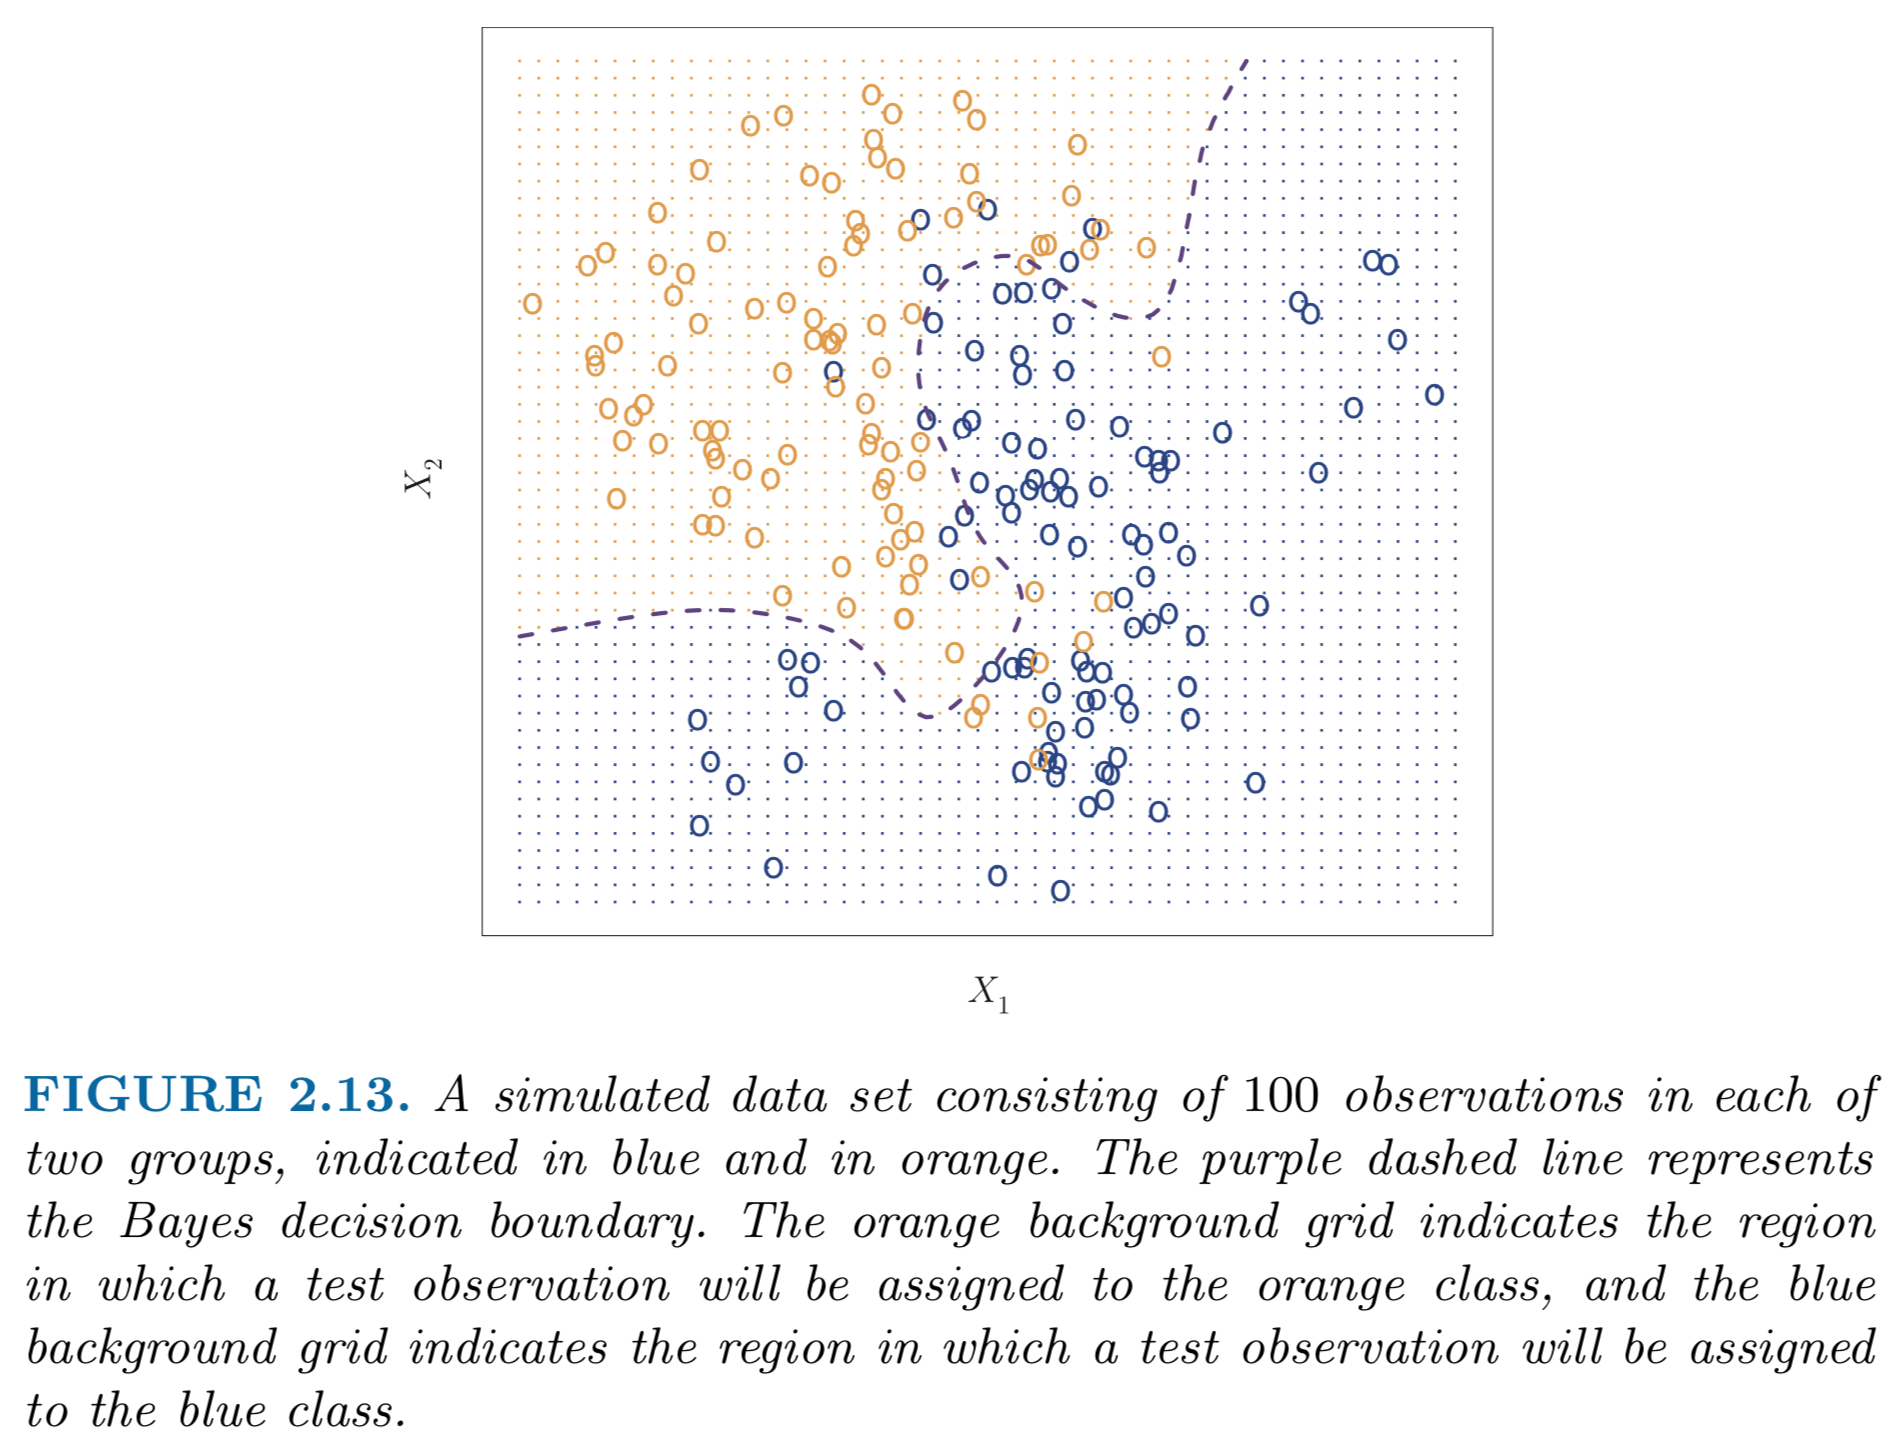
\includegraphics[scale=0.3]{src/ISLR-KNN-CLASSIF.png}	
		\item	Les barrière entre les groupes sont les \textit{Bayes decision boundaries};
		\item[]	Dans le cas de deux classes, il n'en a qu'une seule comme on peut voir;
		\item	On note qu'il y a des mauvaises classifications;
		\item	Puisque le classificateur de Bayes maximise $\Pr(Y = j | X = x_{0})$, le \textit{taux d'erreur de Bayes} est $1 - \underset{j}{\max} \Pr(Y = j | X = x_{0})$;
		\item	En général, le taux d'erreur globale prends la moyenne des probabilités pour toutes les valeurs possible de $X$:
			\begin{align*}
			1 - \text{E}[\underset{j}{\max} \Pr(Y = j | X = x_{0})]
			\end{align*}
		\item	On peut penser au taux d'erreur de Bayes comme l'erreur irréductible en régression;
	\end{itemize}
%%%	
	\item	\textbf{KNN classifier}
	\item[]	\textbf{Mise en garde} avec Bayes
	\begin{itemize}
		\item	En réalité, on ne connaît pas la distribution conditionnelle d'$Y$;
		\item	Ce faisant, le classificateur de Bayes sert plus comme un \textit{golden standard} auquel on peut comparer d'autres méthodes;
		\item	Les autres méthodes \textit{estiment} la probabilité conditionnelle puis classifient avec la valeur maximale \textit{estimée};
	\end{itemize}
	\item[]	Classification avec KNN
		\begin{enumerate}[label = \roman*.]
		\item	Sélectionner un nombre entier $K$;
		\item	Considérer les valeurs de $Y$ pour les $K$ points les plus près;
		\item	Poser:
			\begin{align*}
			\Pr(Y = j | X = x_{0})	
			=	\frac{\text{nombre de points où } Y = j }{\text{nombre de points } K}
			\end{align*}
		\item	Assigner la valeur de $Y$ avec le classificateur de Bayes
		\item[]	C'est-à-dire, la valeur la plus présente dans les $K$ points les plus près
		\end{enumerate}
	\item[]	Considérations
		\begin{itemize}
		\item	La valeur de $K$ a un énorme impact;
		\item[]	Si $K$ est \textit{trop faible}, la classification n'est \textit{pas assez flexible};
		\item[]	Si $K$ est \textit{trop élevée}, la classification est \textit{trop flexible} (overfitting);
		\item	Pour exemple :
		
		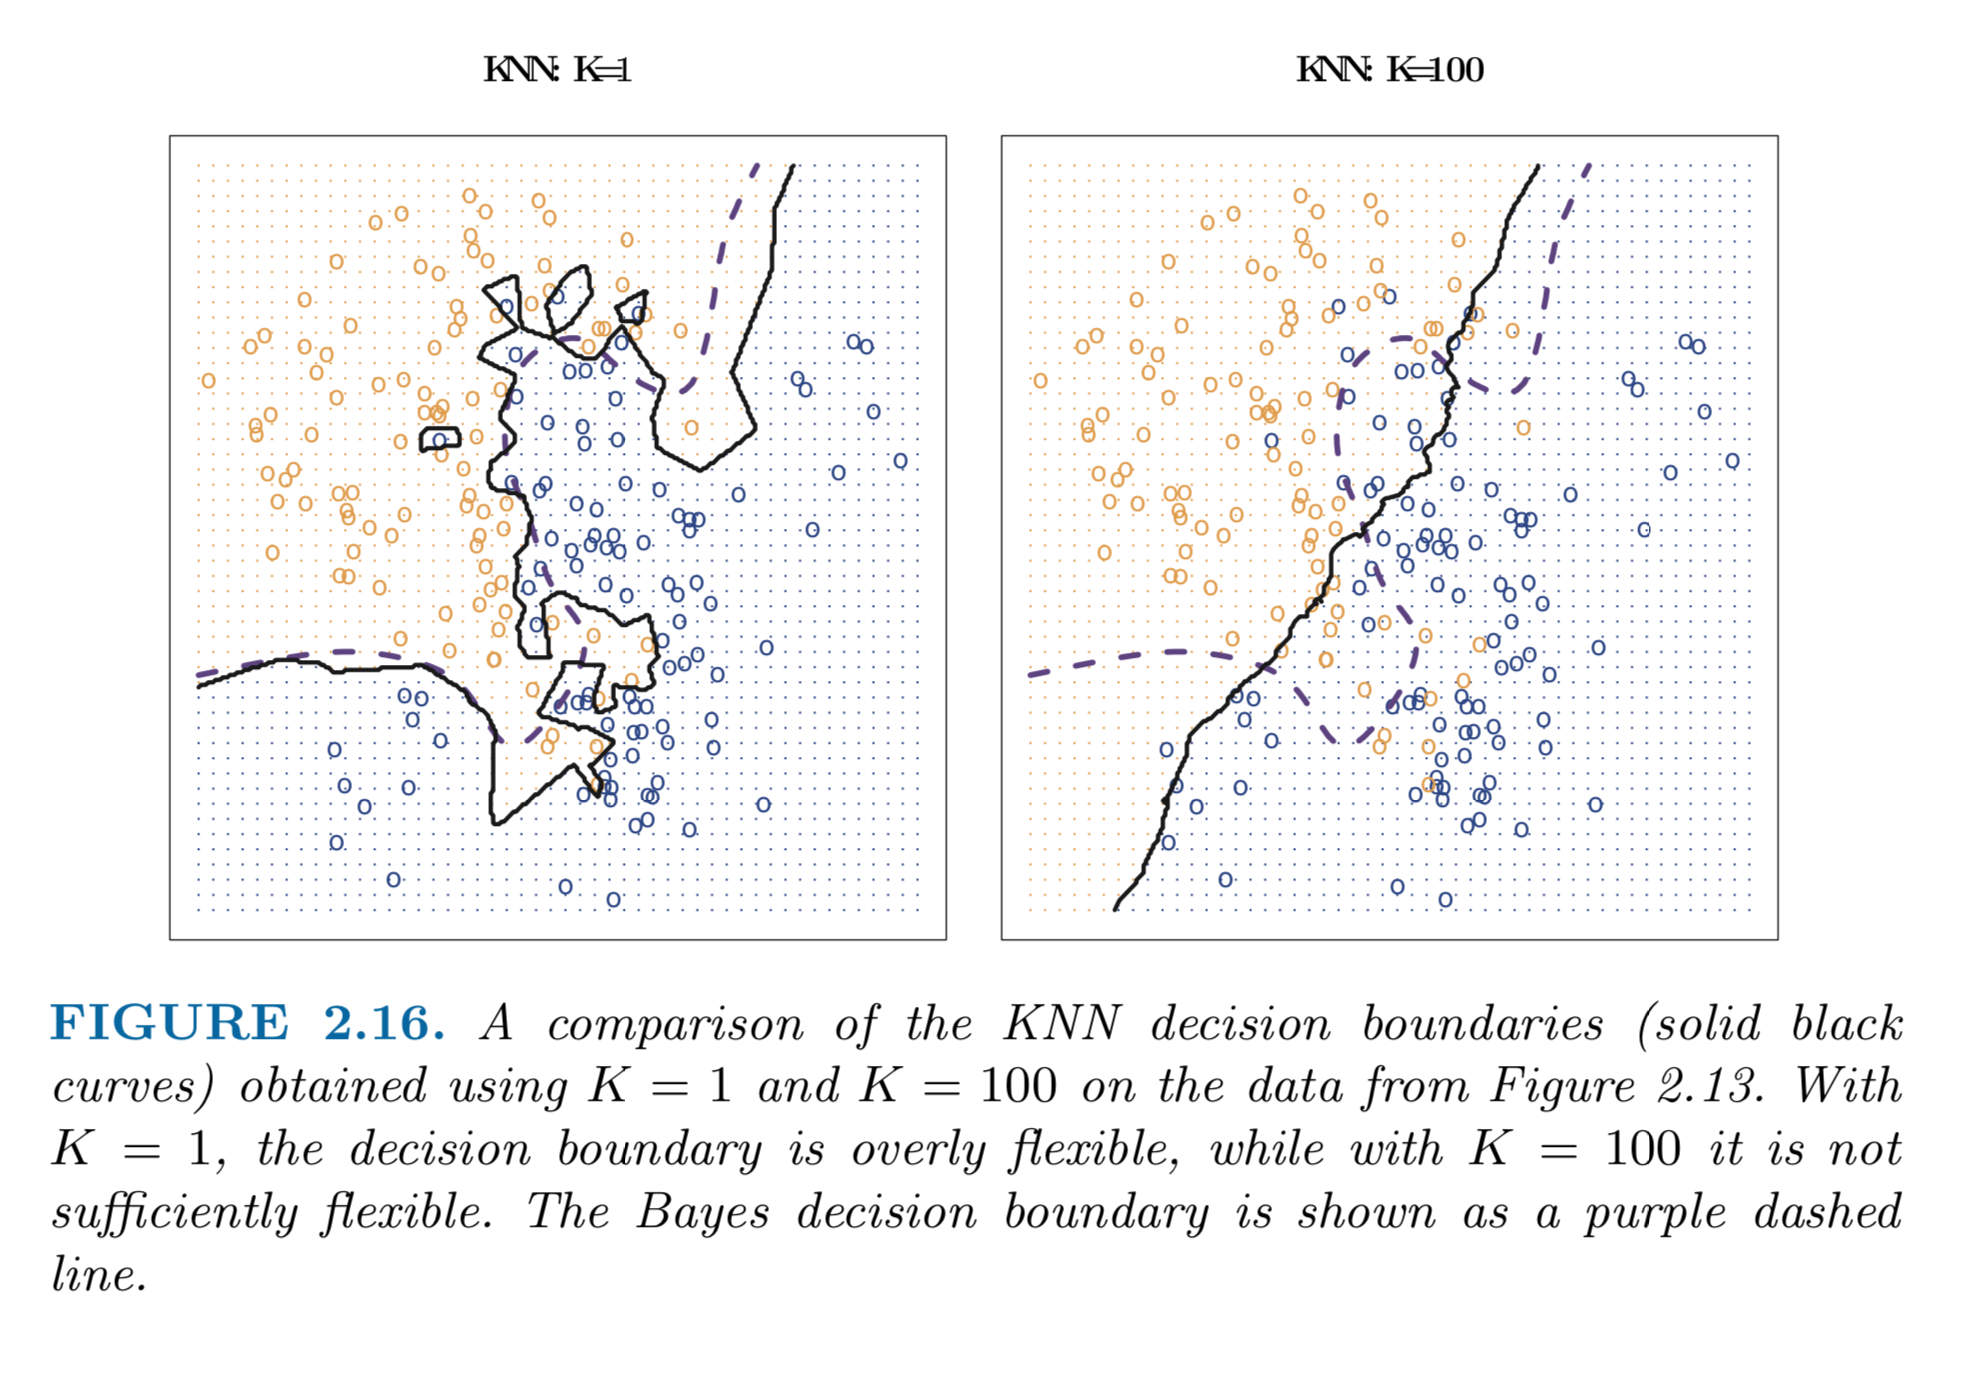
\includegraphics[scale=0.3]{src/ISLR-KNN-CLASSIF-K-choice.png}
		\item	Donc lorsque $K$ augmente, la variance augmente, mais le biais décroît et vice-versa;	
		\end{itemize}
%%%		
	\item	\textbf{Régression KNN}
	\item[]	\textbf{Description}
		\begin{itemize}
		\item	KNN est une méthode non paramétrique qui ne spécifie pas de \textit{functional relation} entre la variable réponse et les variables explicatives;
		\item[]	En contraste, la régression linéaire pose qu'il existe une relation linéaire alors que ceci n'est pas nécessairement le cas;
		\item	En régression KNN, la valeur de $K$ est sélectionné et la valeur de la variable réponse à tout point est la moyenne des valeurs aux $K$ points les plus près;
		\item	La régression va donc donner une \textit{fonction stepwise};
		\end{itemize}
	\item[]	\textbf{Problèmes et considérations}
		\begin{itemize}
		\item	L'impact de $K$ a le même concept qu'en classification;
		\item	Pour exemple : 
		
		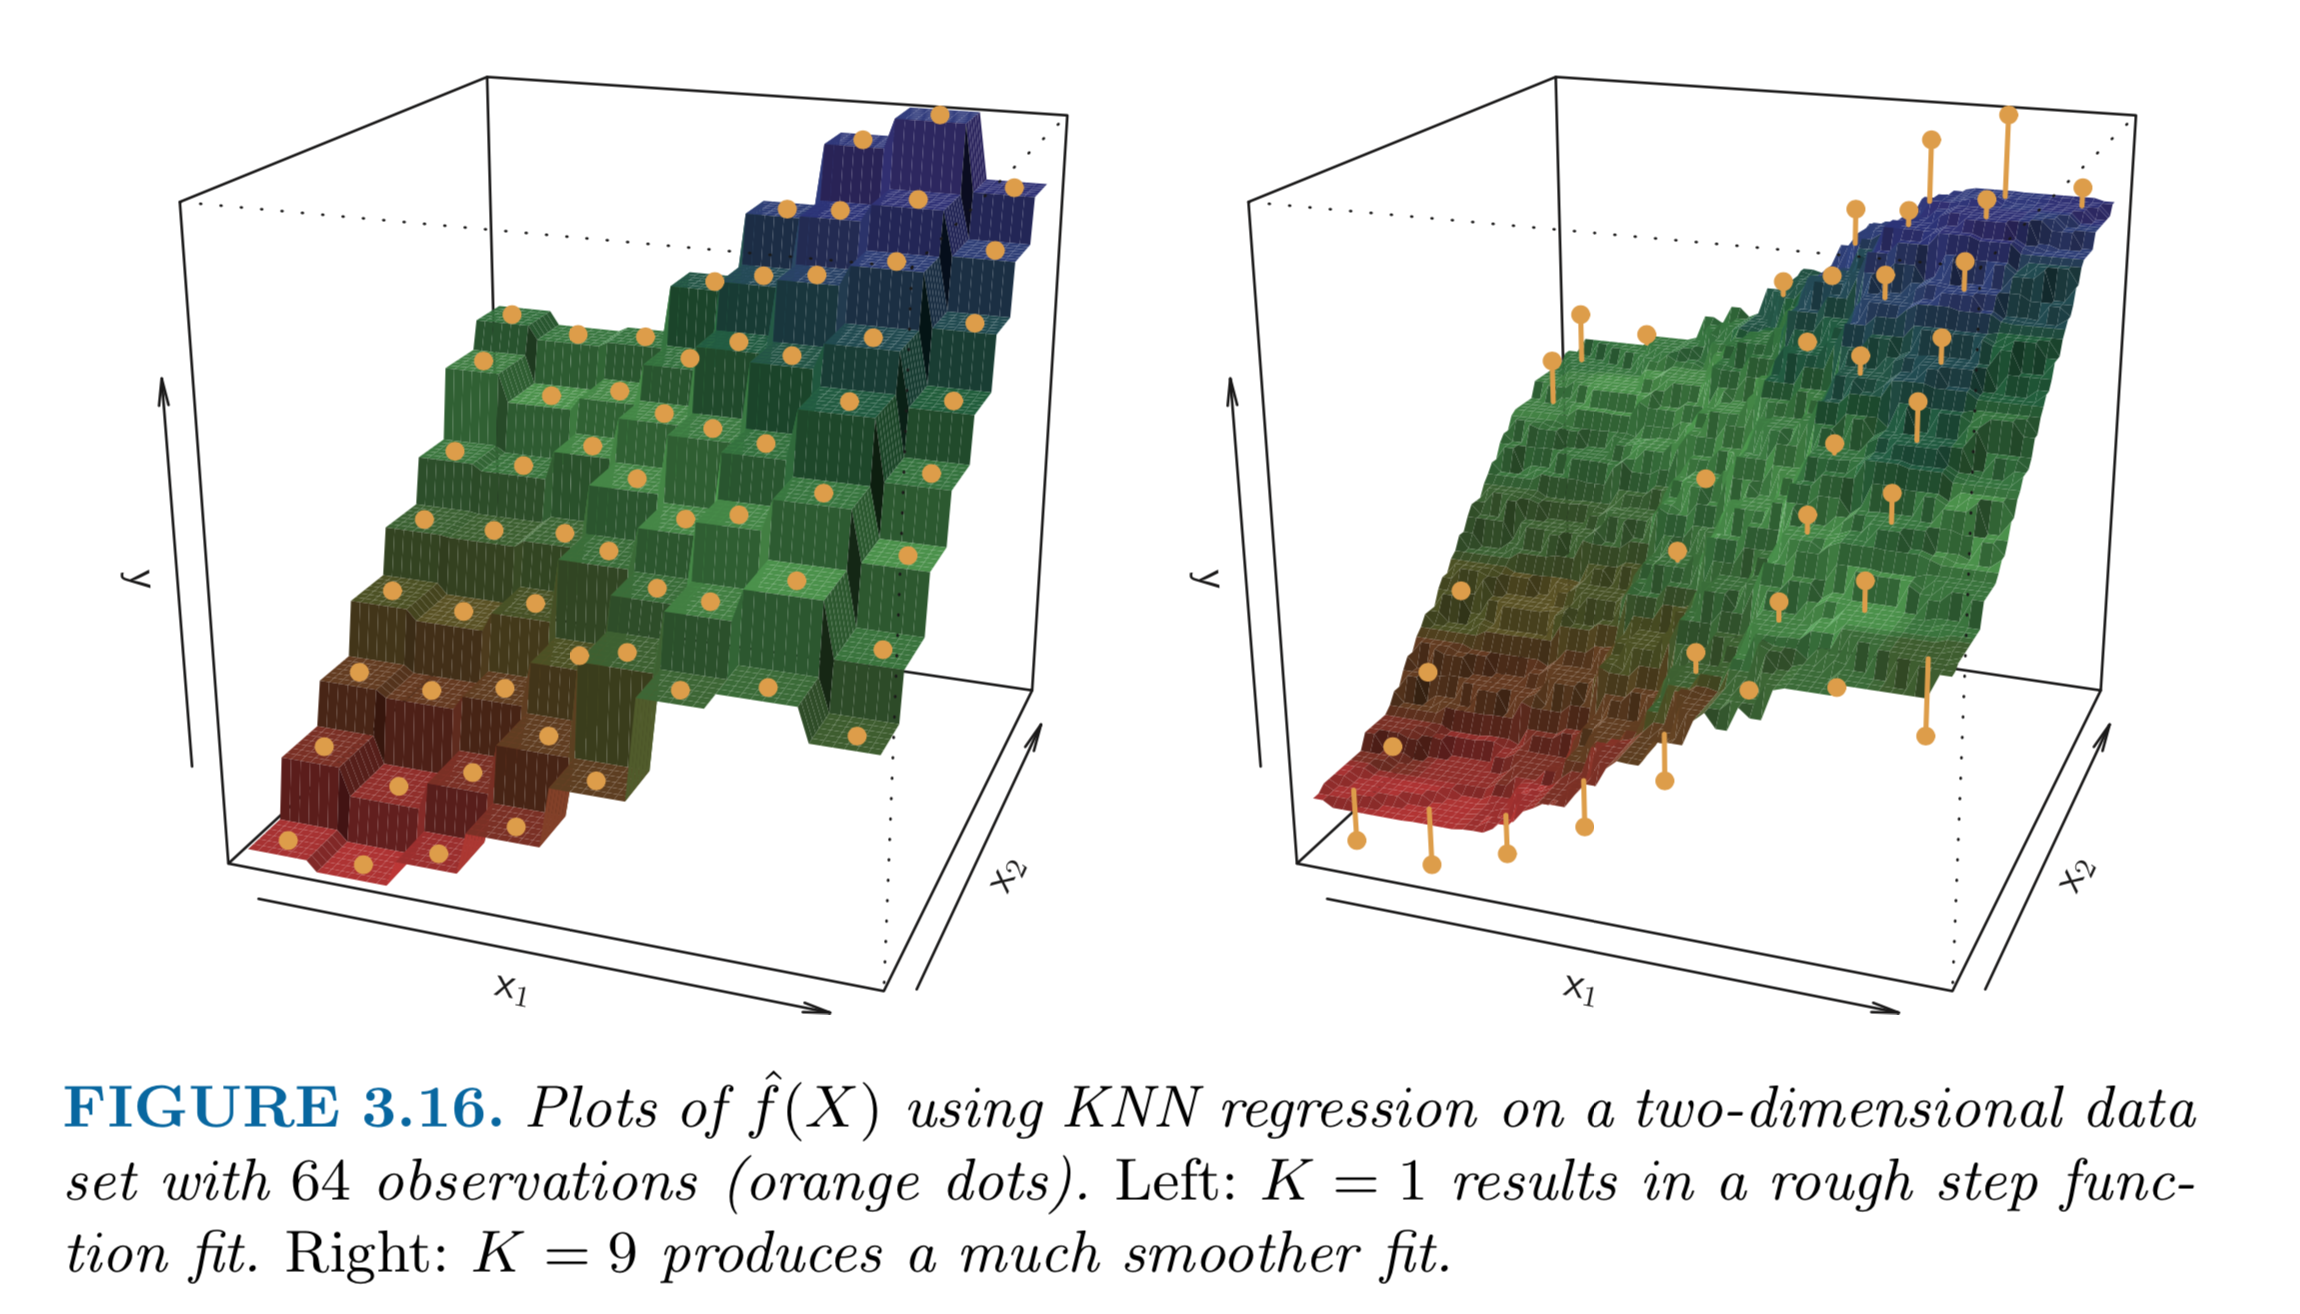
\includegraphics[scale=0.25]{src/ISLR-KNN-CLASSIF-K-regression.png}\label{fig:KNN-3D}
		\item[]	On note donc des points bien moins \textit{smooth} à la gauche qu'à la droite;
		\item[]	La valeur optimale dépend donc encore du trade-off entre le biais et la variance;
		\item	Pour exemple, les prévisions:
		
		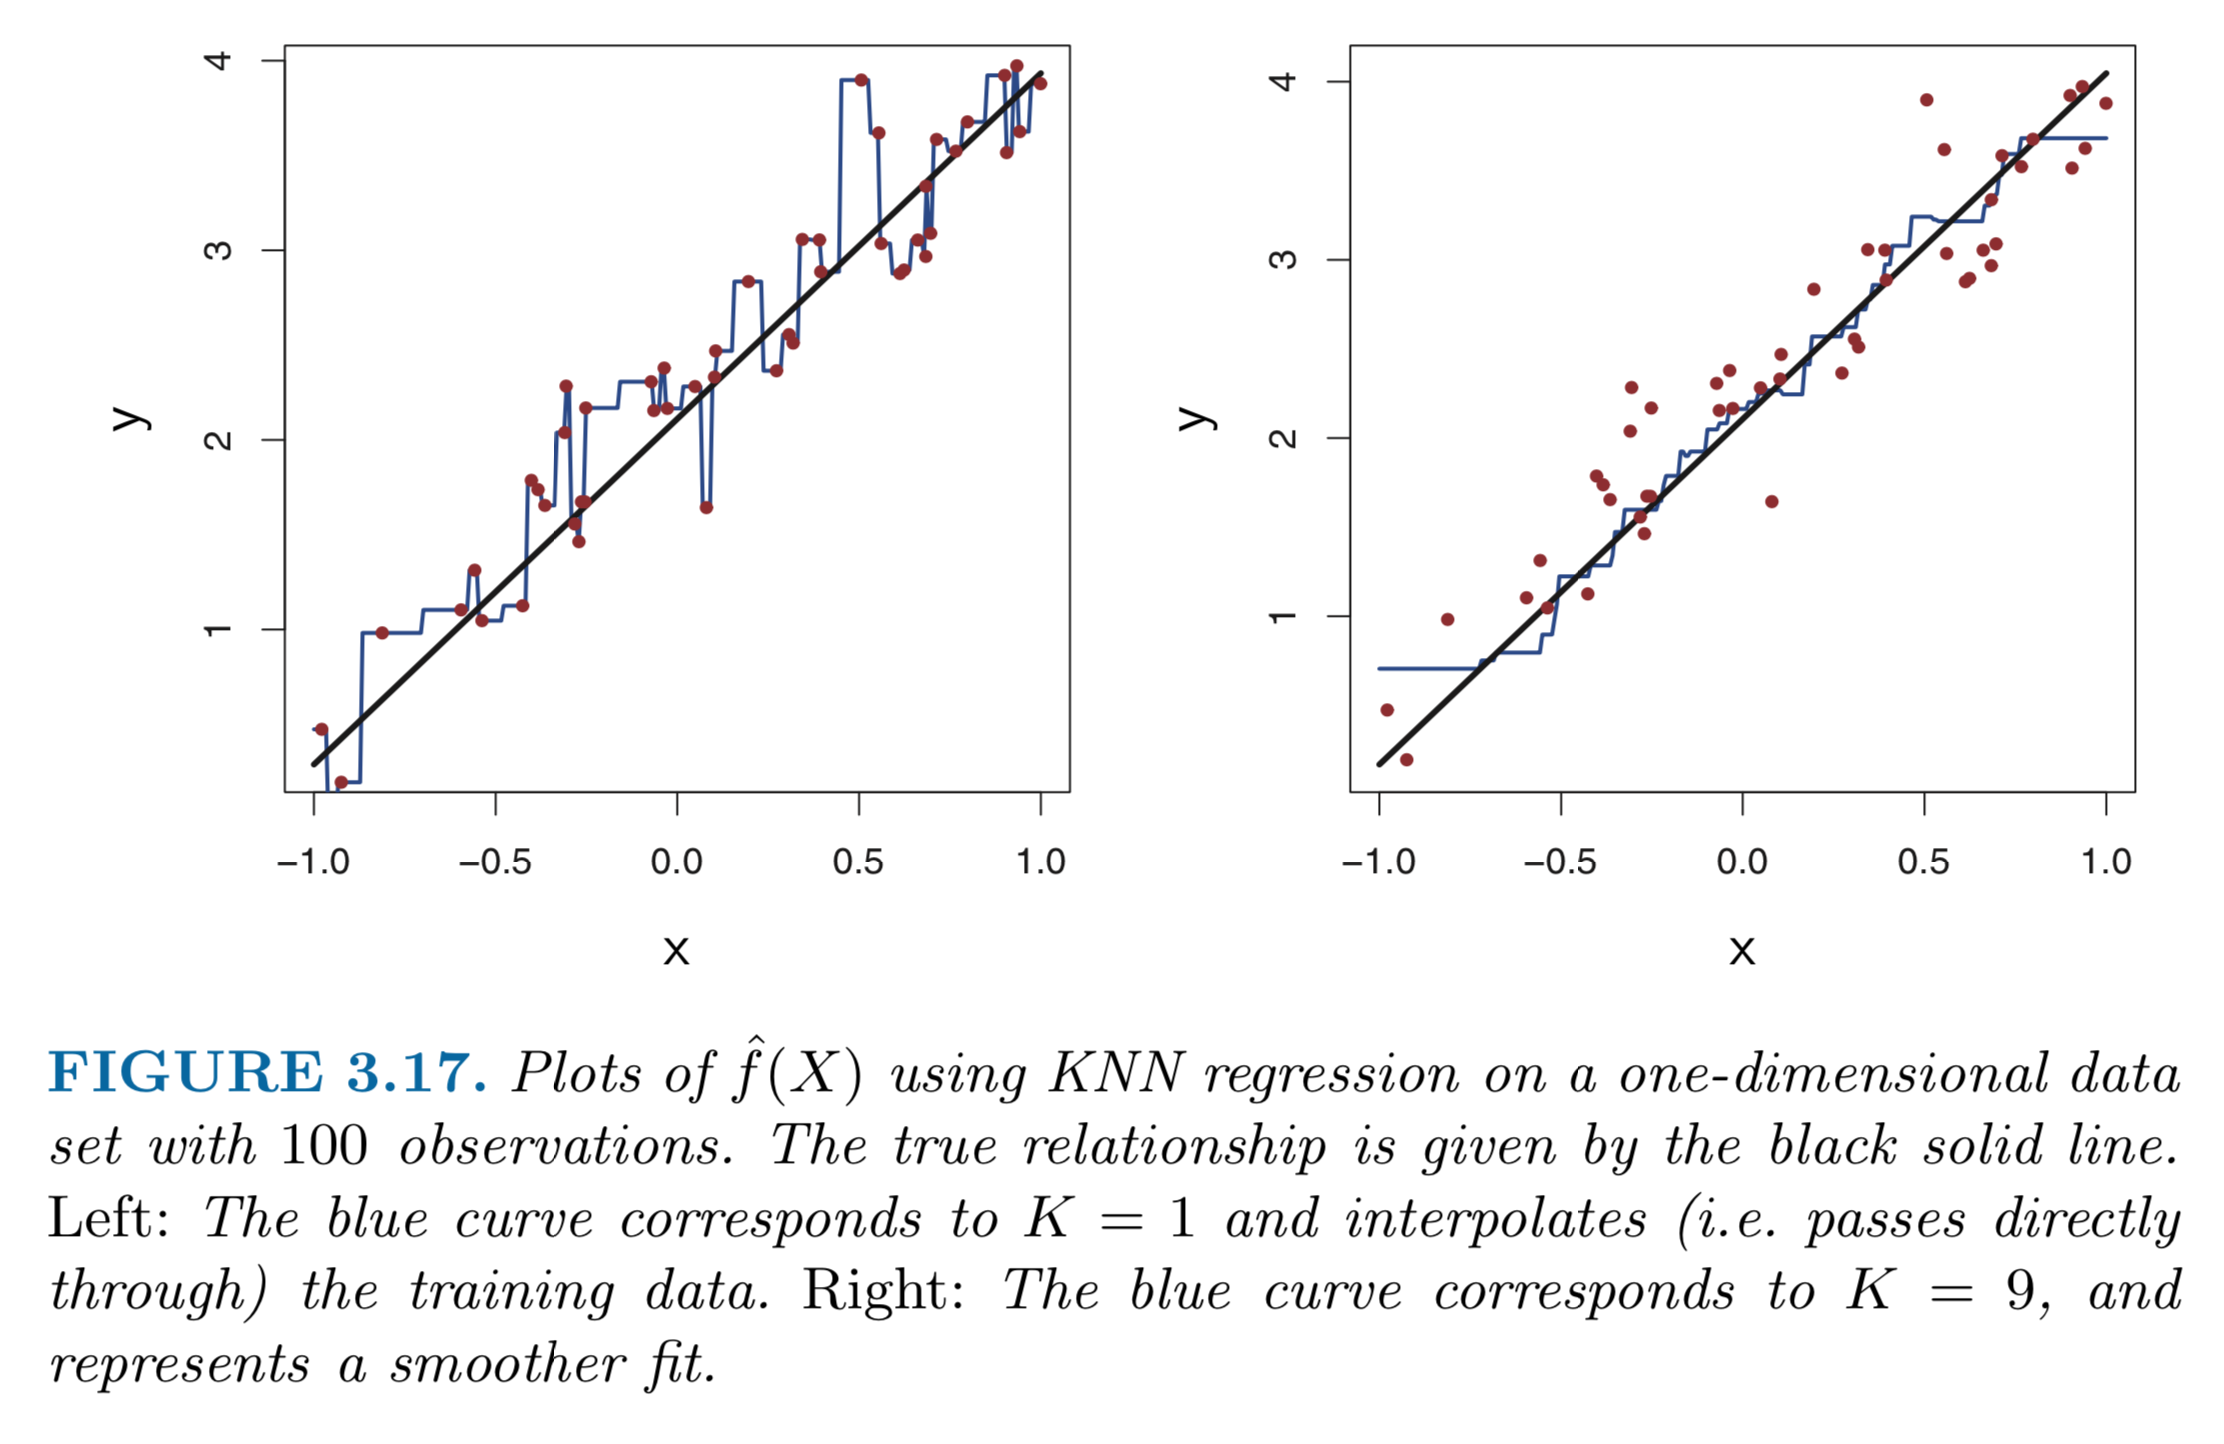
\includegraphics[scale=0.25]{src/ISLR-KNN-CLASSIF-K-regression-LINE.png}
		\item	La meilleure méthode dépend en fait des données;
		\item[]	Si une relation linéaire existe, alors la régression linéaire est mieux et vice-versa;
		\item	Également, il est possible que les $K$ points les plus \textit{près} ne soient pas près du tout et donc que la valeur soit fondée sur des observations très éloignées;
		\item	De plus, la régression linéaire est plus simple à interpréter;
		\end{itemize}
\end{enumerate}
\textbf{Note sur les exercices:} Généralement:
\begin{enumerate}
	\item	Questions reliées à Bayes 
		\begin{itemize}
		\item	Calculer un le taux d'erreur de Bayes (1, 2, 3);
		\item[]	Particulièrement avec une densité ou des probs ce qui nous force à vraiment comprendre les bornes et tout;
		\item	Isoler une decision boundary
		\item[] Particulièrement avec plus de 2 groupes qui nécessite plus de compréhension (4, 5);
		\end{itemize}	
	\item	Semble probable qu'il y aura des questions qualitatives comme le numéro 6;
	\item	Questions reliées au $K$-NN 
		\begin{itemize}
		\item	Calculer des prévisions (7, 8)
		\item	Calculer des taux d'erreurs (9);
		\item	\textbf{Faire la régression} (10, 11);
		\end{itemize}
	\item	Pour ma part, j'ai de la misère à comprendre les calculs mais par la fin j'ai catché;
	\item[]	Cela dit, va falloir que je refais les exercices pour vraiment comprendre;
	\item[]	La théorie n'est pas compliqué, faut juste conceptualiser les calculs, bornes, etc.;
\end{enumerate}
\end{CHPT_SUMM}

\newpage

\chapter[Time Series Models]{Time Series Models (12.5\% à 17.5\%)}

\subsection{Information}

\begin{distributions}[Objective]
Understand key concepts concerning regression-based time series models.
\end{distributions}

\begin{outcomes}[Learning outcomes]
\begin{enumerate}
	\item	Définir et expliquer les concepts, et composantes, des processus de séries chronologiques stochastiques. Incluant:
	\begin{itemize}
		\item	Les marches aléatoires
		\item	Stationnarité
		\item	Auto-corrélation
	\end{itemize}
	\item	Décrire des modèles de séries chronologiques précis dont:
	\begin{itemize}
		\item	Exponential smoothing
		\item	Autoregressive (AR)
		\item	Autoregressive Conditionally Heteroskedastic (ARCH et GARCH)
	\end{itemize}
	\item	Calculer et interpréter les valeurs prédites et leurs intervalles de confiance.
\end{enumerate}
\end{outcomes}

\begin{ASM_chapter}[Related lessons ASM]
\begin{enumerate}
  \setcounter{enumi}{18}
	\item	\hyperref[timeseries19]{Time Series: Basics}
	\item	\hyperref[timeseries20]{Time Series: Autoregressive Models}
	\item	\hyperref[timeseries21]{Time Series: Forecasting Models}
\end{enumerate}
\end{ASM_chapter}

\begin{YTB_vids}[Vidéos YouTube]
\begin{itemize}
	\item	\href{https://www.youtube.com/watch?v=7A83lXbs6Ik}{Dr. Daniel Soper: Visualizing Random Walks in Three Dimensions}
	\item	\href{https://www.youtube.com/watch?v=-gmlyRRscXo}{Ben Lambert: Time series vs cross sectional data}
	\item	\href{https://www.youtube.com/watch?v=bWo_ka37szw&list=PLvo9ZnEQG5oXC-cg8ecXr6SJZWprEL1UC&index=3}{Ben Lambert: Time series Gauss Markov conditions}
	\item	\href{https://www.youtube.com/watch?v=LgIOgb-6mYA&list=PLvo9ZnEQG5oXC-cg8ecXr6SJZWprEL1UC&index=3}{Ben Lambert: Strict exogeneity}
	\item	\href{https://www.youtube.com/watch?v=a7_3qX67e7c&list=PLvo9ZnEQG5oXC-cg8ecXr6SJZWprEL1UC&index=4}{Ben Lambert: Strict exogeneity assumption - intuition}
	\item	\href{https://www.youtube.com/watch?v=DeORzP0go5I&list=PLvcbYUQ5t0UHOLnBzl46_Q6QKtFgfMGc3&index=14}{ritvikmath: Time Series Talk : Autocorrelation and Partial Autocorrelation}
	\item	\href{https://www.youtube.com/watch?v=oY-j2Wof51c&list=PLvcbYUQ5t0UHOLnBzl46_Q6QKtFgfMGc3&index=6}{ritvikmath: Time Series Talk: Stationarity}
	\item	\href{https://www.youtube.com/watch?v=cr4zIXAmSRI}{ritvikmath: Time Series Talk : White Noise}
	\item	\href{https://www.youtube.com/watch?v=VPNijQ2L3XM&list=PLvcbYUQ5t0UHOLnBzl46_Q6QKtFgfMGc3&index=4}{ritvikmath: Time Series Talk : Lag operator} \textit{(pas super important pour SRM)}
	\item	\href{https://www.youtube.com/watch?v=5-2C4eO4cPQ}{ritvikmath: Time Series Talk : Autoregressive Model}
	\item	\href{https://www.youtube.com/watch?v=voryLhxiPzE&list=PLvcbYUQ5t0UHOLnBzl46_Q6QKtFgfMGc3&index=6}{ritvikmath: Time Series Talk : Moving Average Model}
%	\item	\href{https://www.youtube.com/watch?v=_tgB-ri9-8c&list=PLvcbYUQ5t0UHOLnBzl46_Q6QKtFgfMGc3&index=10}{ritvikmath: Time Series Talk: Moving Average and ACF}
	\item	\href{https://www.youtube.com/watch?v=HhvTlaN06AM&list=PLvcbYUQ5t0UHOLnBzl46_Q6QKtFgfMGc3&index=9}{ritvikmath: Time Series Talk: ARMA Model}
	\item	\href{https://www.youtube.com/watch?v=3UmyHed0iYE&list=PLvcbYUQ5t0UHOLnBzl46_Q6QKtFgfMGc3&index=9}{ritvikmath: Time Series Talk: ARIMA Model}
	\item	\href{https://www.youtube.com/watch?v=Li95a2biFCU&list=PLvcbYUQ5t0UHOLnBzl46_Q6QKtFgfMGc3&index=8}{ritvikmath: Time Series Talk: ARCH Model}
%	\item	\href{https://www.youtube.com/watch?v=4hrMdu9CSQs&list=PLvcbYUQ5t0UHOLnBzl46_Q6QKtFgfMGc3&index=3}{ritvikmath: Time Series Talk: What is seasonality?}
	\item	\href{https://www.youtube.com/watch?v=WjeGUs6mzXg&list=PLvcbYUQ5t0UHOLnBzl46_Q6QKtFgfMGc3&index=2}{ritvikmath: Time Series Talk: Seasonal ARIMA Model}
\end{itemize}
\end{YTB_vids}

\subsection{Résumés des chapitres}

\begin{CHPT_SUMM}[label = {timeseries19}]{\addcontentsline{toc}{subsubsection}{19. Time Series: Basics}19. Time Series: Basics}
Time series -> Séries chronologiques
\begin{enumerate}
	\item	\textbf{Introduction}
	\item[]	\textbf{Séries chronologiques}
		\begin{itemize}
		\item	Série d'observations $y_{1}, y_{2}, \dots, y_{T}$ sur des intervalles de temps consécutives;
		\item	L'analyse de séries chronologiques consiste à essayer de déchiffrer des patterns dans les séries pour en faire des prévisions;
		\item[]	Ces patterns peuvent prendre plusieurs formes y inclut de relier les observations $y_{t}$ aux observations précédentes de la série ou, au temps lui-même;
		\end{itemize}
	\item[]	\textbf{Données}
		\begin{itemize}
		\item	\textbf{Longitudinales}: Données d'un processus variant avec le temps;
		\item	\textbf{Transversales (cross-sectional)}: l'inverse, elles ne sont pas organisées chronologiquement;
		\item	Pour bien saisir la distinction, on peut visualiser des données \textbf{transversales comme une image} et des \textbf{longitudinales comme une vidéo};
		\item	La différence entre des données chronologiques vs transversales est bien expliquée dans le vidéo de Ben Lambert;
		\end{itemize}
	\item[]	\textbf{Modèle} de 
		\begin{itemize}
		\item	\textbf{causalité}: Sans variables explicatives reliées au temps;
		\item[]	\textcolor{darkterracotta}{Négatif}: les modèles de causalité dépistent la \textbf{corrélation} et \emph{pas} la causalité;
		\item[]	\textcolor{darkterracotta}{Négatif}: les modèles de causalité doivent connaître les valeurs des variables indépendantes pour faire des prévisions sur la variable dépendante;
		\item	\textbf{série chronologique}: L'inverse.
		\item[]	\textcolor{ao(english)}{Positif}: Les modèles de séries chronologiques peuvent trouver des relations causales avec le temps;
		\end{itemize}
	\item[]	\textbf{3 composantes} aux séries chronologiques :
		\begin{enumerate}
		\item	\textbf{Trend} $T_{t}$: Long term pattern des données;
		\item	\textbf{Seasonality} $S_{t}$: Cyclical pattern des données;
		\item	\textbf{Random patterns} $\varepsilon_{t}$;
		\end{enumerate}	
	\item[]	\textbf{Tendance} 
		\begin{enumerate}
			\item	Additive: 		$y_{t} = T_{t} + S_{t} + \varepsilon_{t}$
			\item	Multiplicative: 	$y_{t} = T_{t} \times S_{t} + \varepsilon_{t}$
		\end{enumerate}
	\item[]	\textbf{Ajustement et évaluation} :
		\begin{itemize}
		\item	Lorsqu'il y une tendance, ou un cycle, \textbf{saisonnale} on peut ajuster le modèle avec une variable binaire;
		\item	Lorsqu'il y a une transition (\textbf{Regime change}) on peut ajuster le modèle avec une variable binaire égale à 0 avant le point fixé et 1 après;
		\item	Un scatter plot du modèle contre le temps, i.e. un \textbf{time series plot}, permet d'évaluer la série chronologique. 
		Pour exemple:
		
		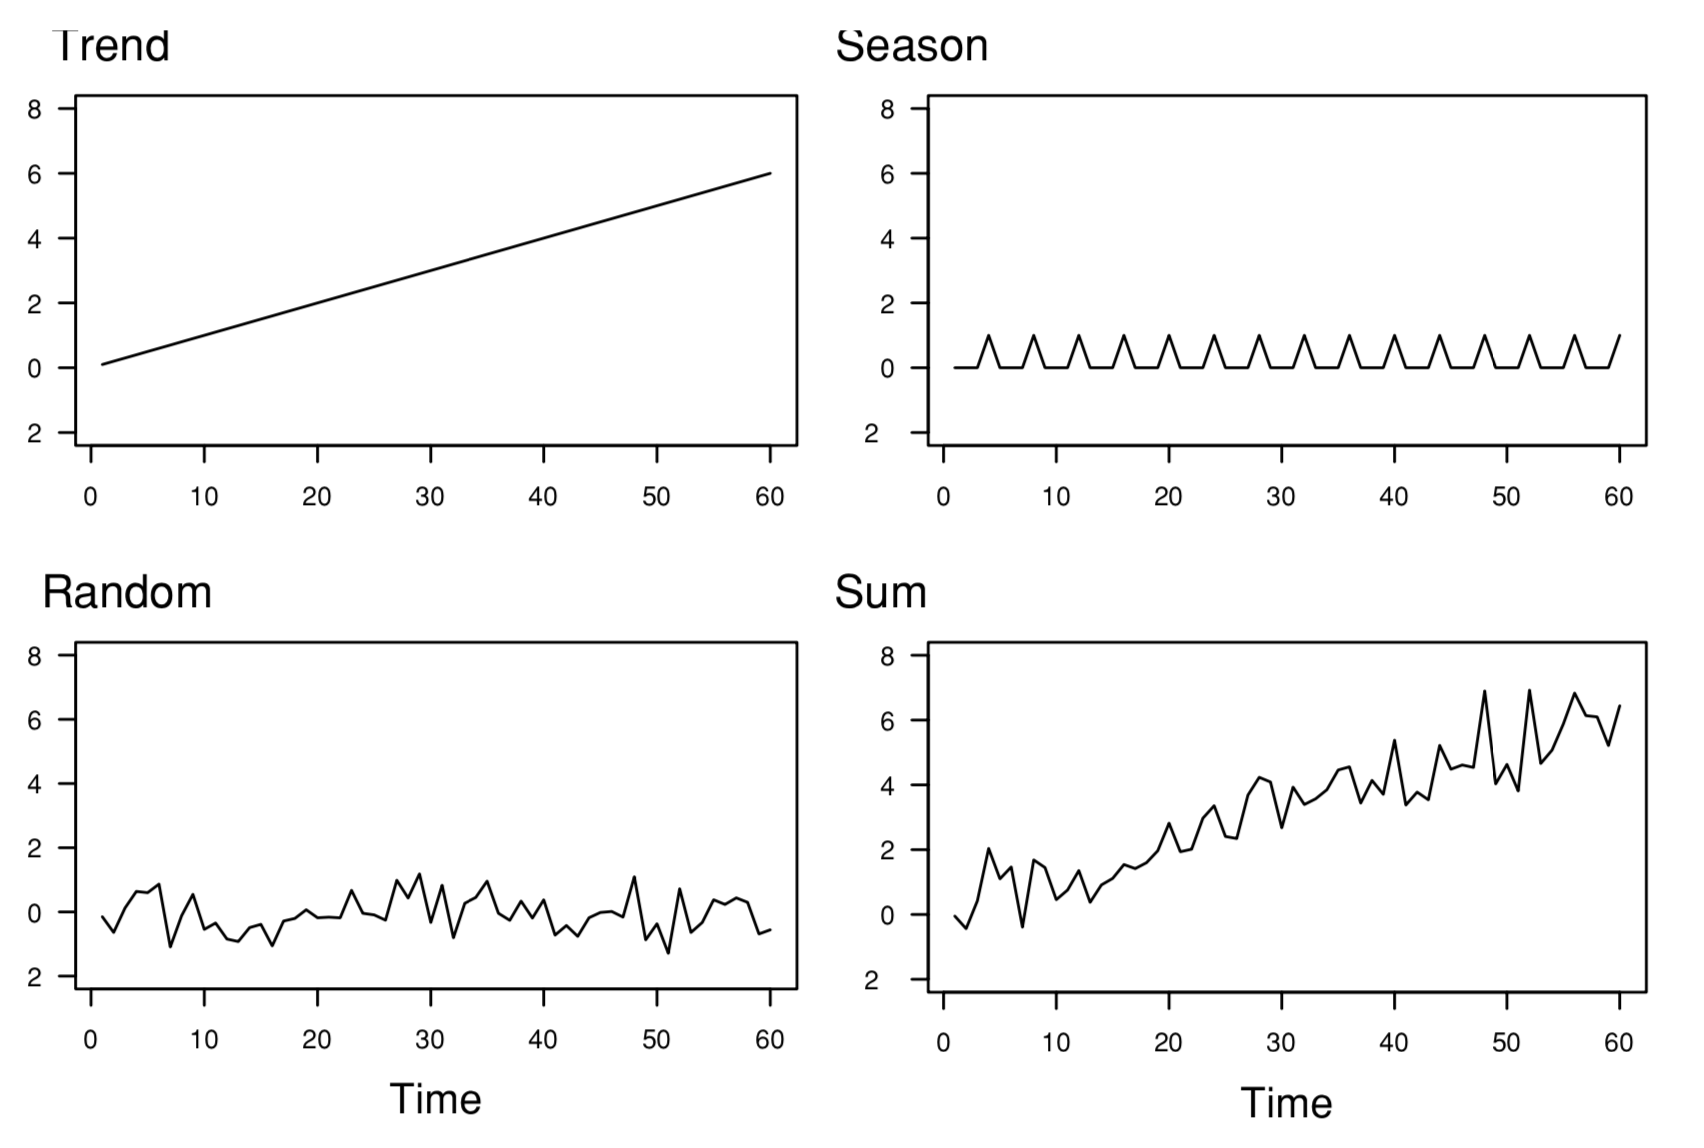
\includegraphics[scale=0.35]{src/time-series-plots.png}
		\end{itemize}
	\item[]	\textbf{Problèmes} :
		\begin{itemize}
		\item	On surnomme parfois les prévisions de séries chronologiques comme étant des prévisions \og \textbf{naïves} \fg{}. 
		\item[]	Les prévisions des modèles de série chronologique prennent en compte uniquement les observations passées pour faire des prévisions;
		\item[]	Elles ne sont \textbf{\textit{ni} ajustées} \textit{ni} \textbf{évaluées} pour des \textbf{relations causales}. 
		\item[]	Ce faisant, elles ne sont pas très représentatives de la réalité et sont \textbf{\textit{naïves}};
		\item	De plus, le modèle de régression va allouer le \textbf{plus de poids aux observations} avec des variables explicatives \textbf{anormalement élevées};
		\item[]	On peut visualiser que si le temps est une variable explicative, alors les données les plus récentes et les plus anciennes seraient les plus éloignées du temps moyen;
		\item[]	\textit{Pour exemple}, si le temps va de 1 à 10 alors le temps moyen est de 5.5 et les points au début et à la fin sont les plus éloignés;
		\item[]	Le modèle va donc attribuer \textbf{plus de poids} aux observations \textbf{récentes et anciennes} qu'aux autres, ce qui n'est pas idéal;
		\item[]	Ce problème est adressé avec du \textbf{smoothing} au chapitre 21;		
		\end{itemize} 
	\item[]	\textbf{Incertitude} des prévisions:
		\begin{itemize}
		\item	Avec des données transversales, le plus éloigné un point est de la masse principale, le moins nous sommes certains des prévisions;
		\item[]	Ce faisant, nous sommes majoritairement intéressés aux prévisions sur des points près de la masse principale;
		\item 	Pareillement, avec des données chronologiques, le plus loin dans le futur une prévision, le moins nous en sommes certains;
		\item[]	Ce faisant, nous sommes majoritairement intéressés aux prévisions d'évènements pas trop loin dans le temps; 
		\end{itemize} 
%%%		
	\item	\textbf{Moyenne} et \textbf{variance}
	\item[]	\textbf{Stationnarité}
		\begin{itemize}
		\item	Si la \textbf{moyenne} \textit{(au temps t)} $\text{E}[y_{t}] = \mu(t)$ ne varie pas dans le temps, la série est \textbf{stationnary in the mean};
		\item[]	Ce faisant, on peut l'estimer avec les valeurs observées;
		\item	Pareillement, si la \textbf{variance} \textit{(au temps t)} $\text{Var}(y_{t}) = \sigma^{2}(t)$ ne varie pas dans le temps, la série est \textbf{stationnary in the variance};
		\item[]	Ce faisant, on peut l'estimer avec la variance échantillonnale;
		\item	Cependant, lorsque les données sont corrélées (ce à quoi on s'attend) alors la variance échantillonnale va \textbf{sous-estimer} la vraie variance;
		\item	L'\textbf{auto-corrélation, ou \textit{serial correlation})} est mesuré par la corrélation échantillonnale;
		\item[]	À noter que la sous-estimation de la variance devient de moins en moins importante plus la taille de la série augmente;
		\item	La distance $k$ des observations d'une série chronologique au temps $t$ avec la même série au temps $t + k$ est le \textbf{lag};
		\item	Si la série a une espérance stationnaire et que la variance et corrélation sont fonction seulement du \textit{lag}, et non du temps lui-même, alors la série est dite \textbf{\textit{(weakly)} stationary} \textbf{(par défaut)};
		\item	Si aucun des moments plus élevés ne varie avec le temps, alors la série est \textbf{\textit{strongly} stationary};
		\end{itemize}
%%%		
	\item	\textbf{White noise}: Une série chronologique \textbf{white noise}  $w_{t}$ est caractérisé par:
	\begin{itemize}
		\item	L'indépendance des termes;
		\item[]	Ce faisant, la corrélation $r_{k}$ à tous \textbf{lag} \textit{supérieurs à 0} est de 0 ($r_{0}$ est toujours égale à 1);
		\item	Une espérance constante $\mu_w$;
		\item[]	Habituellement, elle est nulle;
		\item	Une variance constante $\sigma^{2}_w$;
		\item	Habituellement, on suppose également la normalité;
	\end{itemize}
%	
	\item[]	Réduction de série alias \textbf{time series \textit{filtering}}:
		\begin{itemize}
		\item	Nous cherchons toujours à réduire toute série chronologique à une série white noise en \textbf{identifiant des patterns};
		\item	Pour visualiser ce que le time series filtering représente, on observe ces graphiques d'ondes sonores d'instruments:
		
		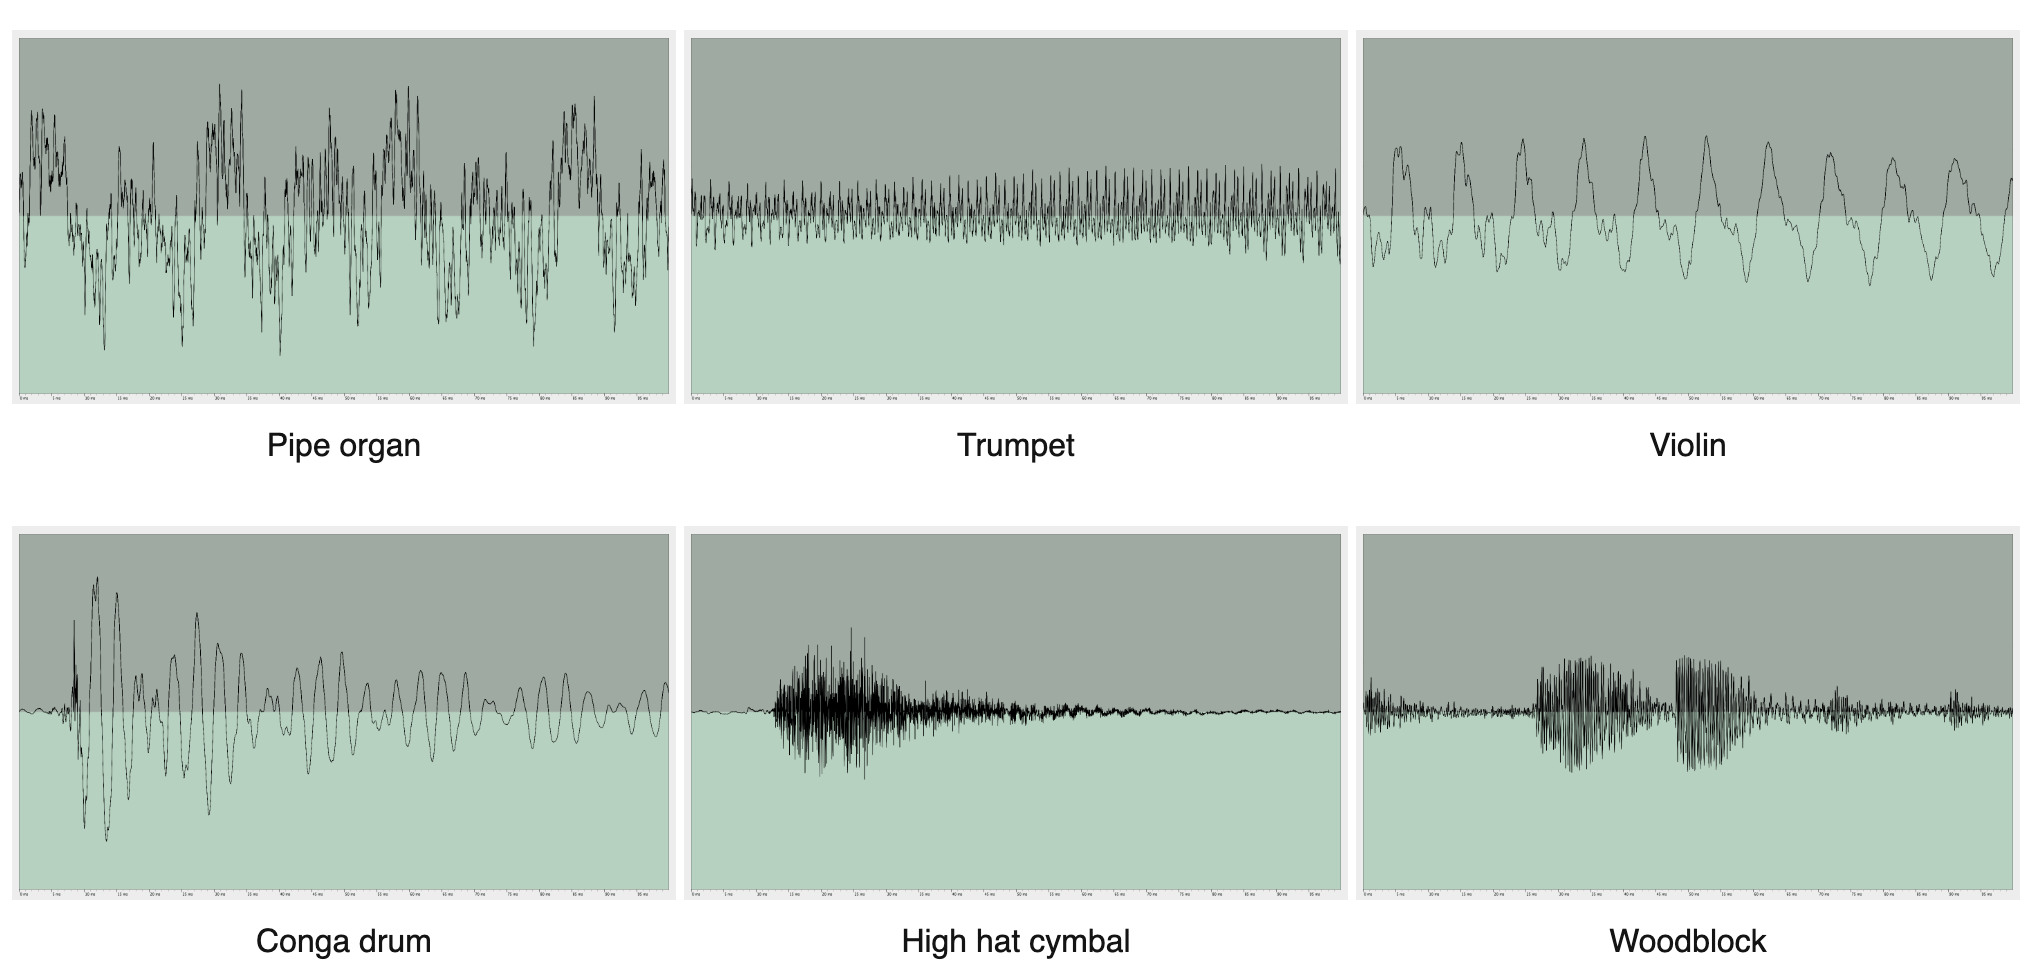
\includegraphics[scale=0.3]{src/music-waves.png}
		\item[]	Et si nous avions une combinaison de ces fréquences:
		
		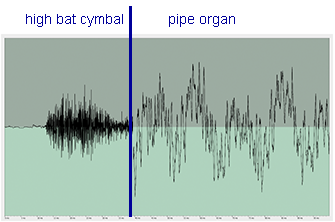
\includegraphics[scale=0.6]{src/regime-change-wave.png}
%		\item	Sans annotations, on pourrait peut-être porté à croire qu'il n'y a pas de tendances dans certaines de ces images;
		\item	Cette idée d'observer des tendances dans des graphiques d'ondes sonores est exactement la même idée que le \textit{time series filtering};
		\item[]	On cherche à identifier des tendances, des cycles, des changements de régime, etc. dans une série pouvant sembler d'être aléatoire;
		\item	Dans le même ordre d'idée, lorsqu'un musicien joue son instrument on imagine que ce n'est pas parfait et qu'il y a un certain niveau d'erreur!
		\item[]	Ceci est donc le \textbf{white noise}, l'erreur aléatoire de la fréquence observée à la fréquence attendue;
		\item[]	Alors, pour néanmoins reconnaître une fréquence d'instrument imparfait, on alloue une variabilité (ou déviance) à la série \og parfaite \fg{};
		\item	La partie inexplicable par les patterns qui demeure est dite d'être \textbf{irréductible} et est donc traitée comme du \textbf{\textit{white noise}};
		\end{itemize}
%		
	\item[]	\label{sec:ex_rand_walk} \textbf{Exemples théoriques} de \textbf{filtering}: 
		\begin{itemize}
		\item	Différencier une marche aléatoire (voir ci-dessous);
		\item	Prendre le log de la série. Ceci peut stabiliser la variance;
		\item	Finalement, prendre le log de la différence des séries qui correspond \textit{approximativement} à des changements proportionnels;
		\end{itemize}
%%%
	\item	\textbf{Marches aléatoires}: Une \textbf{marche aléatoire} est:
		\begin{itemize}
		\item	Une série chronologique \textbf{\textit{non}-stationnaire};
		\item	Ayant comme valeur le niveau initial $y_{0}$ en plus de l'accumulation du \textit{white noise} $w_{t}$;
		\item	L'expression est donc de la forme: $y_{t} = y_{t - 1} + w_{t}, t \ge 1$.
		\end{itemize}
%		
	\item[]	\textbf{Notes} sur l'\textit{espérance} et la \textit{variance}:
		\begin{itemize}
		\item	Si $\mu_{c} = 0$ la série est néanmoins non-stationnaire puisque la variance croît avec le temps;
		\item	Si $\mu_{w} \neq 0$ la série est une marche aléatoire \textbf{avec drift} où $\mu_{w}$ est le drift;
		\item	On déduit de plus que la différence entre marches aléatoires $y_{t} - y_{t - 1}$ est du white noise;
		\end{itemize}
	\item[]	Pour distinguer et comprendre la distinction entre une tendance dans le temps (à gauche) et une marche aléatoire (à droite) on compare les deux:
	\begin{align*}
		y_{t}	&= 	y_{0} + t k + \varepsilon_{t}	&
		&\text{vs}	&
		y_{t}	&= 	y_{0} + t \mu_{w}  + \sum_{j = 1}^{t} \varepsilon_{j}	
	\end{align*}
	D'où on peut voir le lien entre l'erreur d'un modèle causal et d'un modèle chronologique. Malgré une espérance identique, si $k = \mu_{w}$ la variance de la série chrono va croître avec le temps;
%%%		
	\item	\textbf{Control charts}: Graphiques pour observer l'évolution d'un processus avec le temps.
		\begin{itemize}
		\item	Les données sont placées en ordre chronologique;
		\item	Le graphique comporte une ligne centrale et deux lignes pour les bornes supérieures et inférieures (typiquement Q1 et Q3);
		\item	L'axe des y sert à évaluer la moyenne du processus et l'axe des x permet d'observer l'étendu;
		\item	Ce faisant, l'utilité est un peu semblable à celle d'un boxplot:
			\begin{itemize}
			\item	On évalue si un processus est relativement stable en observant leur distribution relative au temps;
			\item	En revanche, un boxplot permet vérifier que les données n'ont pas trop de points aberrants et qu’elles ne sont pas trop répandues;
			\item	On peut donc évaluer si un processus est stable (en contrôle) ou instable (hors de contrôle);
			\end{itemize}
		\end{itemize}
	\item[]	\textbf{Xbar charts}: Calculer la moyenne des séries de $k$ observations.
		\begin{itemize}
		\item	Pour exemple avec $k = 5$, on calcule la moyenne des observations 1 à 5, 6 à 10, 11 à 15, etc.;
		\item	Puisque la variance des moyennes sera plus faible que la variance de la série, des tendances inhabituelles devraient être plus apparentes;
		\end{itemize}
	\item[]	\textbf{R charts}: Calculer l'étendu des séries de $k$ observations.
		\begin{itemize}
		\item	L'étendu est la valeur maximale - la valeur minimale;
		\item	Ceci donne une idée de la dispersion des données pour évaluer la volatilité et évaluer des patterns;
		\end{itemize}
	\item[]	Exemple de xbar plot:
	
	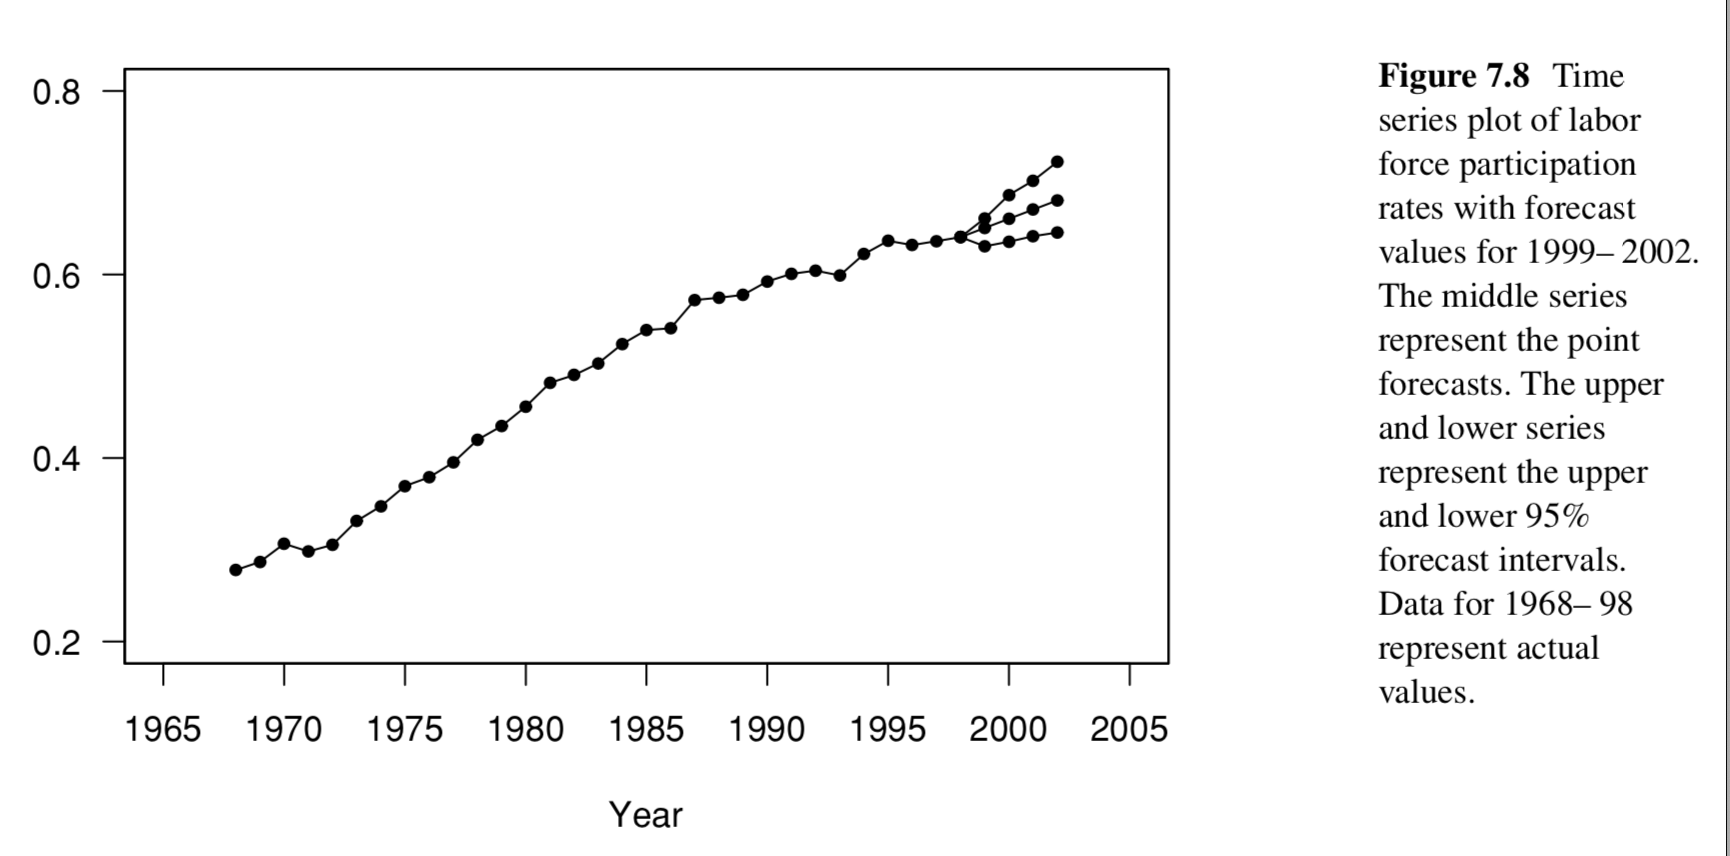
\includegraphics[scale=0.35]{src/xbar-plots.png}
%%%	
	\item	\textbf{Evaluating forecasts} \textit{(évaluer les prévisions)}
	\item[]	On utilise le \textbf{out-of-sample validation}
		\begin{itemize}
		\item	Les données sont partitionnées jusqu'au point fixe $T_{1}$ où $T_{1} < T$;
		\item	Ces données sont utilisés pour ajuster le modèle et le reste pour le tester;
		\item	Avec les données de test on calcule le résidu $e_{t} = \hat{y}_{t} - y_{t}$;
		\end{itemize}
	\item[]	Par la suite on évalue la qualité du modèle avec ces statistiques \emph{(voir formules)}:
	\begin{itemize}
		\item	Le \textbf{Mean Error} (ME) et \textbf{Mean Percentage Error} (MPE) détectent des \textbf{trend patterns};
		\item	\textbf{Cependant}, ils ne \textbf{détectent pas} des problèmes lorsque les \textit{résidus sont positifs et négatifs} avec une \textit{moyenne faible} alors que les \textbf{autres mesures oui};
		\item	De plus, MPE ne peut pas être utilisé lorsque la série contient des 0s et peut être incohérente avec des termes négatifs;
		\item	Le \textbf{Mean Square Error} (MSE) et \textbf{Mean Absolute Error} (MAE) adressent le problème de résidus nuls avec ME et le \textbf{Mean Absolute Percentage Error} (MAPE) pour le MPE;
		\item	Cependant, le MAPE a les même problèmes que le MPE avec les termes nuls;
	\end{itemize}
\end{enumerate}
\textbf{Note sur les exercices:} 
\begin{enumerate}
	\item	Systématiquement les examens de la CAS ont une question où il faut calculer le sample correlation pour un tableau de données dont fort probable ce sera dans SRM (1 à 6);
	\item	Question qu'il faut trouver la prévision ou l'écart-type (d'ailleurs, 2 des sample questions de SRM portent sur ceci);
	\item	Question qualitative sur les propriétés (stationnarité, prévisions, homogénéité, etc.);
	\item	Question comme 17 à 20 dont il faut calculer une des statistiques pour un random walk ou du white noise;
	\item	Avec un peu de réflexion la logique derrière les 5 formules devient évidente et il n'est pas nécessaire de les mémoriser;
\end{enumerate}
\end{CHPT_SUMM}

\begin{FORMULA_SUMM}{Formules chapitre 19}
%\textbf{ASTUCE}: La corrélation échantillonnale peut être calculé avec la TI-30XS. $r_{k} = \frac{\sum XY}{\sum X^{2}}$ où la colonne des $X$ exclue le  premier terme et la colonne des $Y$ le dernier.

\begin{align*}
	s^{2}	&=	\frac{\sum_{t = 1}^{n}(y_{t} - \bar{y})^{2}}{n - 1}	&
	r_{k}	&=	\frac{\sum_{t = k + 1}^{T}(y_{t - k} - \bar{y})(y_{t} - \bar{y})}{\sum_{t = 1}^{T}(y_{t} - \bar{y})^{2}}	\\
	r_{0}	&=	1
\end{align*}
\begin{align*}
	\textcolor{amethyst}{M}E	
	&=	\frac{1}{\textcolor{amethyst}{T - T_{1}}} \sum_{t = T_{1} + 1}^{T} e_{t}	&
	\textcolor{amethyst}{M}\textcolor{teal}{P}E	
	&=	\frac{\textcolor{teal}{100}}{\textcolor{amethyst}{T - T_{1}}} \sum_{t = T_{1} + 1}^{T} \frac{e_{t}}{\textcolor{teal}{y_{t}}}	\\
	\textcolor{amethyst}{M}\textcolor{lava}{S}E	
	&=	\frac{1}{\textcolor{amethyst}{T - T_{1}}} \sum_{t = T_{1} + 1} e_{t}^{\textcolor{lava}{2}}	\\
	\textcolor{amethyst}{M}\textcolor{burntorange}{A}E	
	&=	\frac{1}{\textcolor{amethyst}{T - T_{1}}} \sum_{t = T_{1} + 1}^{T} {\color{burntorange}\bigg|}e_{t}{\color{burntorange}\bigg|}	&	
	\textcolor{amethyst}{M}\textcolor{burntorange}{A}\textcolor{teal}{P}E	
	&=	\frac{\textcolor{teal}{100}}{\textcolor{amethyst}{T - T_{1}}} \sum_{t = T_{1} + 1}^{T} {\color{burntorange}\bigg|} \frac{e_{t}}{\textcolor{teal}{y_{t}}}{\color{burntorange}\bigg|}	\\
\end{align*}

Une marche aléatoire est définie par $y_{t} = y_{t - 1} + w_{t}$ lorsque $t \ge 1	$. Ce faisant, on peut définir la série de white noise $w_{t} = y_{t} - y_{t - 1}$.

\begin{minipage}[t]{0.5\linewidth}
Pour une série white noise $w_{t}$:
\begin{align*}
	\text{Var}(w_{t})	
		&=	\sigma^{2}_{w}	\\
	\text{E}[w_{t}]	
		&=	\mu_{w}			
\end{align*}
\end{minipage}
\begin{minipage}[t]{0.5\linewidth}
Pour une marche aléatoire $y_{t}$ :
\begin{align*}
	\text{Var}(y_{t})	
		&=	t \sigma^{2}_{w}	\\	
	\text{E}[y_{t}]	
		&=	y_{0} + {\color{burntorange}\underset{\text{drift si } \mu_w \neq 0}{\underbrace{t \mu_{w}}}}		
\end{align*}
\end{minipage}
\noindent
\begin{tabular}{|p{4.5cm}|c|c|}
\hline
\rowcolor[HTML]{21650A} 
		\multicolumn{1}{|c|}{\cellcolor[HTML]{21650A}{\color[HTML]{FFFFFF} \textbf{Measure}}}                
	&	\multicolumn{1}{c|}{\cellcolor[HTML]{21650A}{\color[HTML]{FFFFFF} \textbf{White noise}}}	
	&	\multicolumn{1}{c|}{\cellcolor[HTML]{21650A}{\color[HTML]{FFFFFF} \textbf{Random walk}}}	\\	
\hline
\rowcolor[HTML]{B8F0A5}	Estimated standard error		&	$se_{\hat{y}_{T + l}} = s_{y}\sqrt{1 + \frac{1}{T}}$	&	$se_{\hat{y}_{T + l}} = s_{w}\sqrt{l}$ 	\\ \hline
\rowcolor[HTML]{B8F0A5}	$l$-period lookahead forecast &	$\hat{y}_{T + l} = \bar{y} \; \forall l$	&	$\hat{y}_{T + l} = y_{T} \textcolor{burntorange}{+ l \bar{w}}$	\\	
\hline
\rowcolor[HTML]{B8F0A5}	Forecast interval of $y_{T + l}$	&	$\bar{y} \pm t_{T - 1, 1 - \frac{\alpha}{2}} s_{y}\sqrt{1 + \frac{1}{T}}$	&	\\	
\hline
\rowcolor[HTML]{B8F0A5}	\parbox{4.5cm}{\textbf{Approximate} 95\% forecast interval of $y_{T + l}$}	&	$\bar{y} \pm 2 s_{y}$	&	$\bar{y} + l \bar{w} \pm 2 s_{w} \sqrt{l}$	\\	
\hline
\end{tabular}
où $\bar{w}$ est la moyenne échantillonnale de $w_{t}$.

\end{FORMULA_SUMM}

\begin{CHPT_SUMM}[label = {timeseries20}]{\addcontentsline{toc}{subsubsection}{20. Time Series: Autoregressive Models}20. Time Series: Autoregressive Models}
Le chapitre 19 couvre l'identification de \textbf{patterns majeures} comme première étape pour faire des prévisions. Le chapitre 20 couvre l'identification de \textbf{tendances plus subtiles} et les modèles pour les accommoder.

\begin{enumerate}
	\item	Introduction
	\item[]	\textbf{Description}
		\begin{itemize}
		\item	Tout comme nous avons l'\textit{auto}-corrélation, nous avons les modèles \textbf{\textit{auto}régressifs};
		\item[]	On applique alors le même concept d'utiliser les valeurs précédentes de la série pour prévoir les prochaines;
		\item	\textbf{Modèle}
		\begin{align*}
			y_{t}	&=	\beta_{0} + \beta_{1} y_{t - 1} + \varepsilon_{t}
		\end{align*}
		\end{itemize}
	\item[]	\textbf{Stationnarité} et liens
		\begin{itemize}
		\item	On note que si $\beta_{1} = 1$ alors la série est une marche aléatoire et est non-stationnaire;
		\item	Également, si $\beta_1 = 0$ alors la série est du white noise;
		\item	Pour assurer la stationnarité, on veut donc $0 < |\beta_{1}| < 1$;

		\item[]	Ce faisant, le domaine de $\beta_{1}$ implique que le modèle auto-régressif sera stationnaire sans être une série white noise;
		\end{itemize}
	\item[]	Comment déterminer qu'un modèle auto-régressif est approprié
		\begin{enumerate}[label = \roman*.]
		\item	Utiliser un \textbf{control chart} pour évaluer la stabilité;
		\item[]	Le modèle AR(1) est stationnaire, on s'attend à un graphique relativement stable;
		\item	Utiliser un \textbf{scatterplot} de la dernière valeur contre la valeur présente de la série;
		\item[]	Le modèle AR(1) devrait, par définition, être corrélé avec la valeur précédente;
		\item	Évaluer la structure de l'\textbf{auto-corrélation};
		\item[]	On test que la série n'est pas du white noise ($\rho_{k} \neq 0$). Voir ci-dessous pour l'explication;
		\end{enumerate}
	\item[]	\textbf{Auto-corrélation}
		\begin{itemize}
		\item	On a que $\rho_{k} = \beta^{k}_{1}$ pour le modèle AR(1);
		\item[]	La logique est que la formule est récursive donc on multiplie les $\beta$ jusqu'à ce qu'on arrive à la première valeur de la série : 1;
		\item	Comme mentionné, si $\beta_{1} = 0$ la série est une série white noise;
		\item[]	Cela implique également que $\rho_{k} = 0$;
		\item	Le \textbf{test} sur l'auto-corrélation est donc de tester \textbf{si} $\rho_{k}$ est \textbf{significativement différent de 0};
		\item[]	Cependant, puisque $-1 < \rho_{k} < 1$, cela peut s'avérer difficile;
		\item[] On \textbf{évalue} donc le \textbf{standard error} de l'auto-corrélation plutôt que la corrélation elle-même;
		\setlength{\mathindent}{-1cm}
		\begin{align*}
			&\mathcal{H}_{0}: \text{Pas d'auto-corrélation \textit{(white noise)} et } se(r_{k}) \approx \frac{1}{\sqrt{T}}	\\
			&\mathcal{H}_{a}: \text{Auto-corrélation et } | se(r_{k}) | > \frac{2}{\sqrt{T}}	
		\end{align*}
		\setlength{\mathindent}{1cm}
		\end{itemize}
	\item[]	\textbf{Estimation} des coefficients
		\begin{itemize}
		\item	Pour comprendre l'estimation de $\beta_{1}$ avec un modèle auto-régressif, on rappel la formulation $b_{1} = r_{xy} \frac{s_{y}}{s_{x}}$;
		\item[]	Puisque la variable explicative est l'observation précédente, $s_{x} = s_{y}$ et $b_{1} = r_{xy}$;
		\item[]	La distinction importante est que le \textbf{modèle évolue dans le temps};
		\item[] Donc, nous n'avons pas la corrélation entre 2 différentes variables mais plutôt l'auto-corrélation entre \textbf{même variable à 2 différents moments};
		\item	Puisqu'il est irréaliste d'évaluer l'auto-corrélation $r_{k}$ à tous les moments $k$, $b_{1} \approx r_{1}$;
		\item	Également, on déduit que $\bar{x} = \bar{y}$ et $b_{0} \approx \bar{y} (1 - b_{1})$;
		\item	La série de prévisions, surnommée \textbf{smoothed series}, devient donc $\hat{y_{t}} = b_{0} + b_{1} y_{t - 1}$ et l'erreur $e_{t} = y_{t} - (b_{0} + b_{1} y_{t - 1})$;
		\end{itemize}
	\item[]	\textbf{Variance} et \textbf{prévisions}
		\begin{itemize}
		\item	Voir la boite de formule pour le raisonnement sous-jacent à la formule du MSE;
		\item	On peut généraliser l'équation de prévision pour obtenir la \textbf{\textcolor{amethyst}{$k$-step ahead} prévision} de $y_{T + k}$ avec $\hat{y}_{T + \textcolor{amethyst}{k}} = b_{0} + b_{1} \hat{y}_{T + \textcolor{amethyst}{k - 1}}$;
		\item	Voir le résumé des formules pour comprendre le raisonnement sous-jacent aux formules de prévisions;
		\end{itemize}
\end{enumerate}
\textbf{Note sur les exercices:} 
\begin{enumerate}
	\item	Calculs de base pour faire liens entre variances;
	\item[]	Semble trop basic pour être une question d'exam, les questions qui semble plus être du genre d'examen sont:
	\item	Faire des prévisions de façon récursive;
	\item	Intervalles de confiances / formules de variance de l'erreur	
\end{enumerate}
\end{CHPT_SUMM}

\begin{FORMULA_SUMM}{Formules chapitre 20}
La \textbf{vraie auto-corrélation} au lag $k$ pour un processus AR(1) stationnaire:
\begin{align*}
	\rho_{k}	
		&=	\beta_{1}^{k}	\\
\end{align*}

Estimations des coefficients
\begin{align*}
	b_{0}	
		&\approx		\bar{y} (1 - b_{1})	&
	b_{1}	
		&\approx		r_{1}	\\
\end{align*}

Prévisions
\begin{align*}
	\hat{y}_{t}	
		&=	b_{0} + b_{1} y_{t - 1}	&
	\hat{y}_{T + \textcolor{amethyst}{k}}
		&=	b_{0} + b_{1} \hat{y}_{T + \textcolor{amethyst}{k - 1}}, k \ge 1	\\
	e_{t}	
		&=	y_{t} - (b_{0} + b_{1} y_{t - 1})	\\
\end{align*}

MSE (variance du terme d'erreur):

\begin{minipage}[ht]{0.5\linewidth}
\begin{align*}
	s^{2}
		&=	\sum_{t = \textcolor{teal}{2}}^{T}	\frac{(e_{t} - \bar{e})^{2}}{\textcolor{burntorange}{T - 3}}	\\
	\widehat{\text{Var}}(y_{t})
		&=	\frac{s^{2}}{1 - b_{1}^{2}}
\end{align*}
\end{minipage}
\begin{minipage}[ht]{0.5\linewidth}
\begin{itemize}
	\item	\textcolor{teal}{$e_{1}$ n'existe pas puisque $y_{0}$ n'existe pas et donc il y a seulement $T - 1$ résidus;}
	\item	\textcolor{burntorange}{On pondère par $T - 3$ puisqu'il y a $T - 1$ observations et 2 paramètres à estimer. La formule est donc la même que d'habitude;}
\end{itemize}
\end{minipage}

Prévision:

\setlength{\mathindent}{-1cm}
\begin{minipage}[ht]{0.5\linewidth}
\begin{align*}
	se_{\hat{y}_{T + \textcolor{amethyst}{k}}} 
		&= 	s \sqrt{1 + b_{1}^{2} + \dots + b_{1}^{2\textcolor{amethyst}{(k - 1)}}}	\\
		&=	s \sqrt{\sum_{t = \textcolor{amethyst}{1}}^{\textcolor{amethyst}{k}} b_{1}^{2\textcolor{amethyst}{(t - 1)}}}	\\
	y_{\textcolor{amethyst}{T + k}}
		&\in		\hat{y}_{\textcolor{amethyst}{T + k}} \pm	t_{1 - \frac{\alpha}{2}, \textcolor{teal}{T - 3}} \, se_{\hat{y}_{T + \textcolor{amethyst}{k}}}	
\end{align*}
\end{minipage}
\begin{minipage}[ht]{0.5\linewidth}
\begin{itemize}
	\item	\textcolor{amethyst}{Voir le $k$-step ahead forecast pour comprendre la logique derrière la variance de l'erreur de prévision $\hat{y}_{T + \textcolor{amethyst}{k}}$;}
	\item	\textcolor{teal}{$T - 3$ pour la même raison que ci-dessus;}
\end{itemize}
\end{minipage}
\setlength{\mathindent}{1cm}
\end{FORMULA_SUMM}

\begin{CHPT_SUMM}[label = {timeseries21}]{\addcontentsline{toc}{subsubsection}{21. Time Series: Forecasting Models}21. Time Series: Forecasting Models}
\begin{enumerate}
	\item	\textbf{Moving, \textit{or running}, average} smoothing
	\item[]	\textbf{Description}
		\begin{itemize}
		\item	Modèle très naïf stipulant que \textbf{la prochaine observation} est la \textbf{moyenne} des k \textbf{dernières observations};
		\item	On peut penser à la \textbf{longueur} du moving average, $k$, comme une \textbf{fenêtre} d'observations sur lesquelles on applique le modèle de moving average;
		\end{itemize}
	\item[]	\textbf{Estimation} et \textbf{longueur} $k$ du moving average
		\begin{itemize}
		\item	L'estimation du modèle de moving average est défini comme :
			\begin{equation*}
			\hat{s}_{t}	
				=	\frac{y_{t - (k - 1)} + y_{t - (k - 2)} + \dots + y_{t}}{k}
			\end{equation*}
		Ce qui est essentiellement une reformulation de la moyenne échantillonnale;
		\item	Le plus large la fenêtre $k$, le plus \textit{smooth} le modèle et le plus la moyenne va tendre vers 0;
		\item[]	Également, si $k = 1$ aucun \textit{smoothing} n'est appliqué;
		\item	Pour bien saisir ceci voici un exemple avec $k = 24$ et $k = 12$ d'un modèle de smoothing:
		
		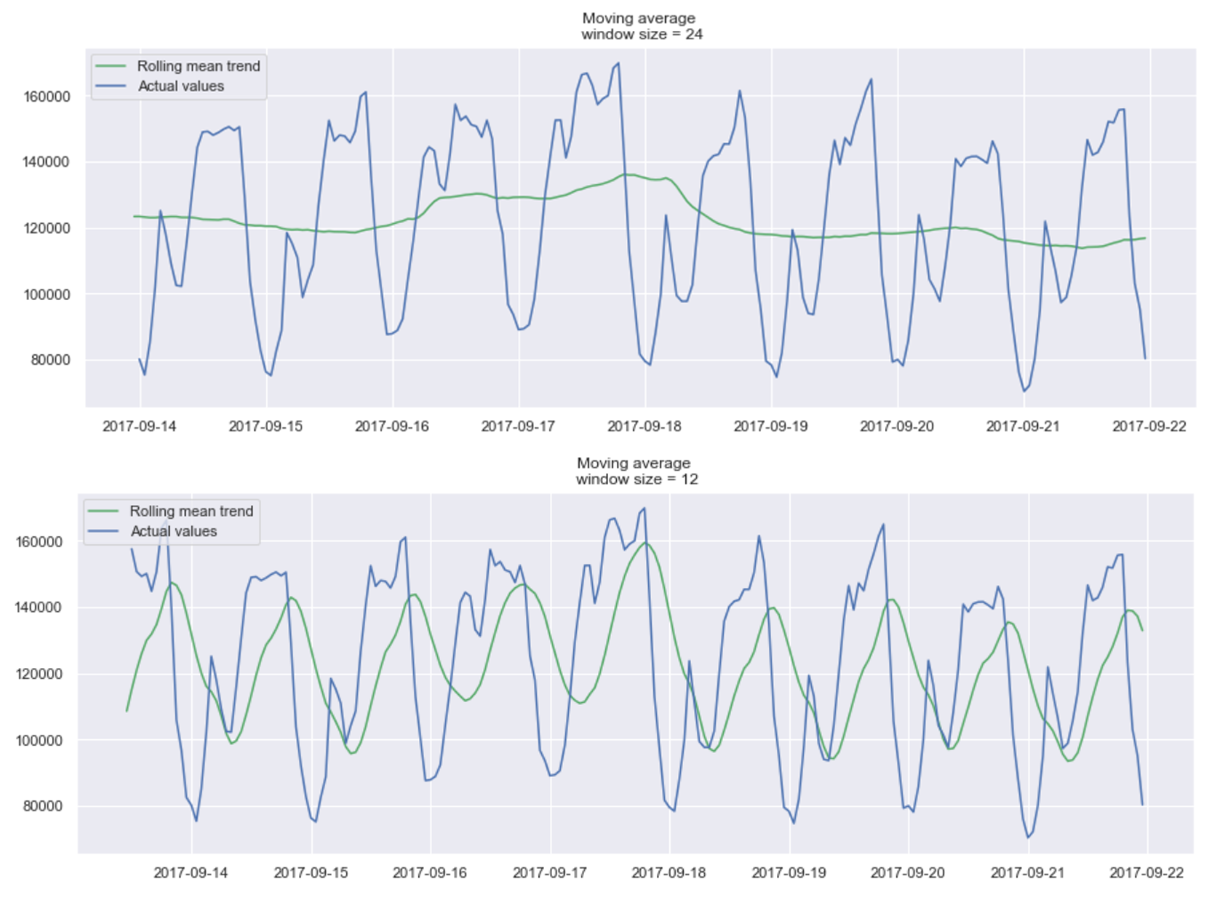
\includegraphics[scale=0.25]{src/smoothing-example.png}
		\item	Un bon exemple de ceci en pratique est l'indice des prix à la consommation pour stabiliser les augmentations et mieux identifier les tendances;
		\item	La balance est donc de bien balancer le $k$ pour identifier les tendances sans faire de \textbf{oversmoothing} et être incapable d'identifier les vraies tendances;
		\end{itemize}
	\item[]	\textbf{Prévisions}
		\begin{itemize}
		\item	La série peut également être réexprimée pour faire des prévisions :
			\begin{equation*}
			\hat{s}_{t}	=	\hat{s}_{t - 1} + \frac{y_{t} - y_{t - k}}{k}
			\end{equation*}
			S'il n'y a pas de tendance, $y_{t} - y_{t - k}$ s'annule et on prévoit $\hat{y}_{T + l} = \hat{s}_{T} \, \forall l$;
		\item	Si un modèle a une tendance linéaire, par exemple $y_{t} = \beta_{0} + \beta_{1} t + \varepsilon_{t}$, on peut le traiter avec du \textit{double smoothing};
		\end{itemize}
	\item[]	\textbf{Procédure} pour obtenir une série \textbf{doubly smoothed}
		\begin{enumerate}
		\item	Créer une \textbf{smoothed series} des valeurs $\hat{s}_{t}^{(1)}$ avec la même formule réécrite ci-dessous:
			\begin{equation*}
			\hat{s}_{t}^{(1)}	
				=	\frac{y_{t} + \dots + y_{t - (k - 1)}}{k}
			\end{equation*}
		\item	Pour	 créer une \textbf{doubly smoothed series}, réappliquer la même formule à la série qui a \textbf{déjà \textit{été smoothed}}:
			\begin{equation*}
			\hat{s}_{t}^{(2)}	
				=	\frac{\hat{s}_{t}^{(1)} + \dots + \hat{s}_{t - (k - 1)}^{(1)}}{k}
			\end{equation*}
		\end{enumerate}
	\item[]	\textbf{Estimations} de \textbf{double smoothing}
		\begin{itemize}
		\item	L'estimation de la tendance est alors
			\begin{equation*}
			b_{1, T}	
				=	\frac{2(\hat{s}_{t}^{(1)} - \hat{s}_{t}^{(2)})}{k - 1}
			\end{equation*}
		\item	Et la prévision $l$ lead times dans le futur :
			\begin{equation*}
			\hat{y}_{T + l}
				=	\hat{s}_{t} + b_{1, T}	
			\end{equation*}
		\end{itemize}
	\item[]	\textbf{Attribution de poids}
		\begin{itemize}
		\item	Le average smoothing est en réalité une \textit{minimisation des moindres carrés \textbf{pondérée}} assignant un poids de 1 pour les observations dans la fenêtre $k$ et de 0 pour les autres;
		\item[]	Ce faisant, il n'est pas optimal d'arbitrairement sélectionner un point $k$ où l'on segmente les données et d'ensuite attribuer le même poids aux observations sélectionnées;
		\item[]	En réalité, on veut donner plus de poids aux observations récentes qu'aux plus vieilles observations;
		\item[]	Allouer un poids décroissant aux observations est précisement ce que fait le \textit{exponential smoothing};
		\end{itemize}	
%%%			
	\item	\textbf{Exponential} smoothing	
	\item[]	\textbf{Lien} avec le moving average smoothing
		\begin{itemize}
		\item	Pour visualiser le lien avec le moving average et avec l'estimation des moindres carrés pondérés, l'expression du \textbf{exponential smoothed estimate} de la série est:
			\begin{equation*}
			\hat{s}_{t}
				=	\frac{y_{t} + w y_{t - 1} + w^{2} y_{t - 2} + \dots + w^{t} y_{0}}{1/(1 - w)}
			\end{equation*}
			d'où l'idée de pondération des observations s'éclaircit;
		\end{itemize}
	\item[]	\textbf{Description}
		\begin{itemize}
		\item	L'\textbf{exponential smoothing} utilise la même logique que le moving average smoothing mais en attribuant un \textbf{poids décroissant};
		\item[] Alias, on attribue plus d'importance aux observations récentes avec de moins en moins d'importance le plus on s'éloigne du présent;
		\item	On peut réécrire l'expression de façon récursive :
			\begin{equation*}
			\hat{s}_{t}
				=	w \hat{s}_{t - 1} + (1 - w) y_{t}
			\end{equation*}
		\item	Le poids (weight), ou \textbf{smoothing factor}, est \textbf{contenu entre 0 et 1} et représente \textbf{la vitesse} à laquelle le poids de l'observation précédente va \textbf{décroître};
		\item[]	Alors, le plus faible $w$, le plus \textit{smooth} la série
		\item[]	Pour concrétiser, en un exemple de différentes poids:
		
		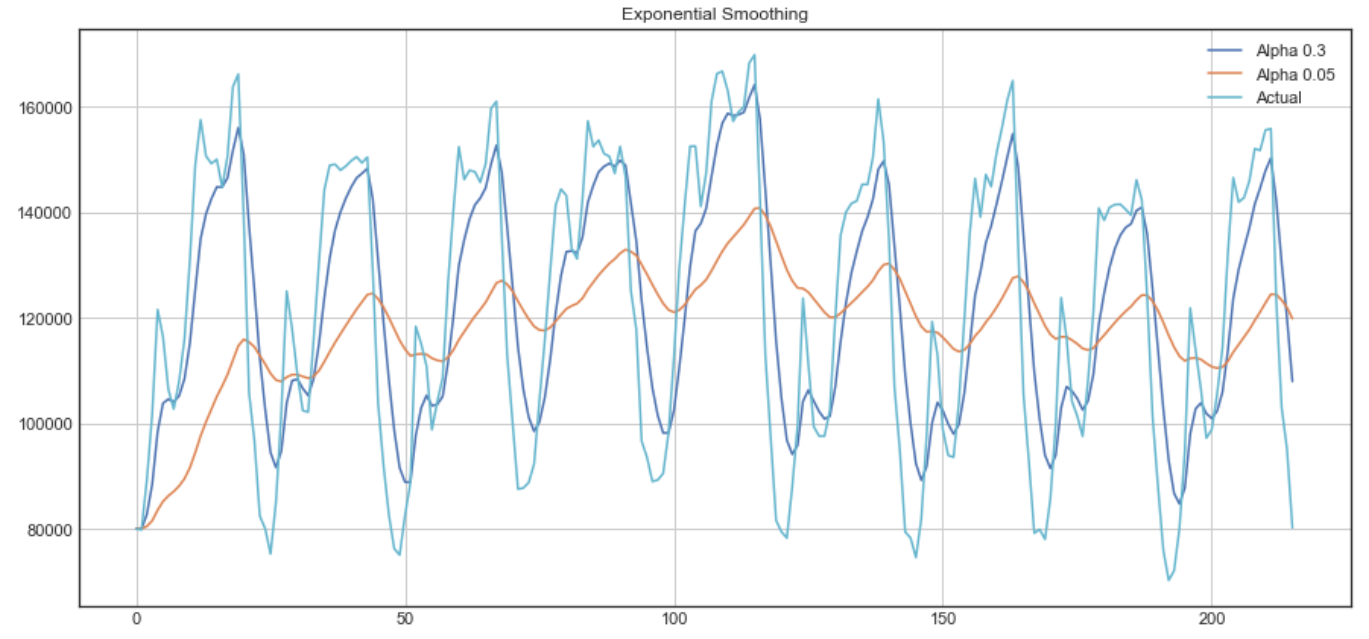
\includegraphics[scale=0.2]{src/exponential-smoothing-example.png}
		\end{itemize}
%		
	\item[]	\textbf{Prévision} de exponential smoothing
		\begin{itemize}
		\item	La prévision $l$ lead times dans le futur :
			\begin{equation*}
			\hat{y}_{T + l}
				=	b_{0, T} + b_{1, T} l
			\end{equation*}
		\item	De plus, le \textbf{one-step ahead prediction error} permet de comparer ce que le modèle aurait prédit dans le passé, $\hat{s}_{t - 1}$, contre les données que nous possédons $y_{t}$:
			\begin{equation*}
			\varepsilon_{t}
				=	y_{t} - \hat{s}_{t - 1}	
			\end{equation*}		
		\item[]	Les \textbf{prévisions} permettent alors d'\textbf{évaluer l'ajustement} du modèle;
		\item	On définit également la \textbf{Sum of Squared one-step ahead prediction error}:
			\begin{equation*}
			SS(w)
				=	\sum_{t = 1}^{T}(y_{t} - \hat{s}_{t - 1})^{2}, \, \hat{s}_{0} = y_{0}
			\end{equation*}
		\item[]	Puisque $SS(w)$ est fonction du poids, on choisit le poids la minimisant $SS(w)$;
		\end{itemize}	
%		
	\item[]	\textbf{Tendances linéaires} et \textbf{double smoothing}
		\begin{enumerate}
		\item[]	Pareillement au moving average smoothing, le présence de tendance linéaire est traitée avec du \textit{double smoothing}
		\item	Créer une \textbf{smoothed series} des valeurs $\hat{s}_{t}^{(1)}$ avec la formule simplifiée réécrite ci-dessous:
			\begin{equation*}
			\hat{s}_{t}^{(1)}	
				=	w \hat{s}^{(1)}_{t - 1} + (1 - w) y_{t}
			\end{equation*}
		\item	Pour	 créer une \textbf{doubly smoothed series}, utiliser l'étape précédente comme input:
			\begin{equation*}
			\hat{s}_{t}^{(2)}	
				=	w \hat{s}^{(2)}_{t - 1} + (1 - w) \hat{s}^{(1)}_{t}
			\end{equation*}
		\end{enumerate}
	\item[]	\textbf{Estimations} de \textbf{double exponential smoothing}
		\begin{itemize}
		\item	L'estimation de la tendance et de l'intercepte est alors
			\begin{align*}
			b_{1, T}	
				&=	\frac{(1 - w)}{w}\left(\hat{s}_{t}^{(1)} - \hat{s}_{t}^{(2)}\right)	\\
			b_{0, T}
				&=	2\hat{s}_{t}^{(1)} - \hat{s}_{t}^{(2)}
			\end{align*}
			où l'équation de l'intercepte est \textit{très semblable} à l'équation de la pente pour le moving average smoothing;
		\item	Et la prévision $l$ lead times dans le futur :
			\begin{equation*}
			\hat{y}_{T + l}
				=	b_{0, T} + b_{1, T} l	
			\end{equation*}
		\end{itemize}
%%%		
	\item	\textbf{Seasonal} models
	\item[]	\textbf{Description}
		\begin{itemize}
		\item	Les modèles de saisonnalité sont habituellement utilisés pour expliquer des phénomènes naturels;
		\item	Par exemple, la position du soleil dans le temps qui dépends de l'heure;
		\item	Ce faisant, les fonctions trigonométriques peuvent être utilisées pour ajuster des modèles avec saisonnalité;
		\item[]	Pour comprendre l'intuition sous-jacente à l'utilisation des fonctions trigonométriques, observer ce graphique de la fonction d'auto-corrélation:
		
		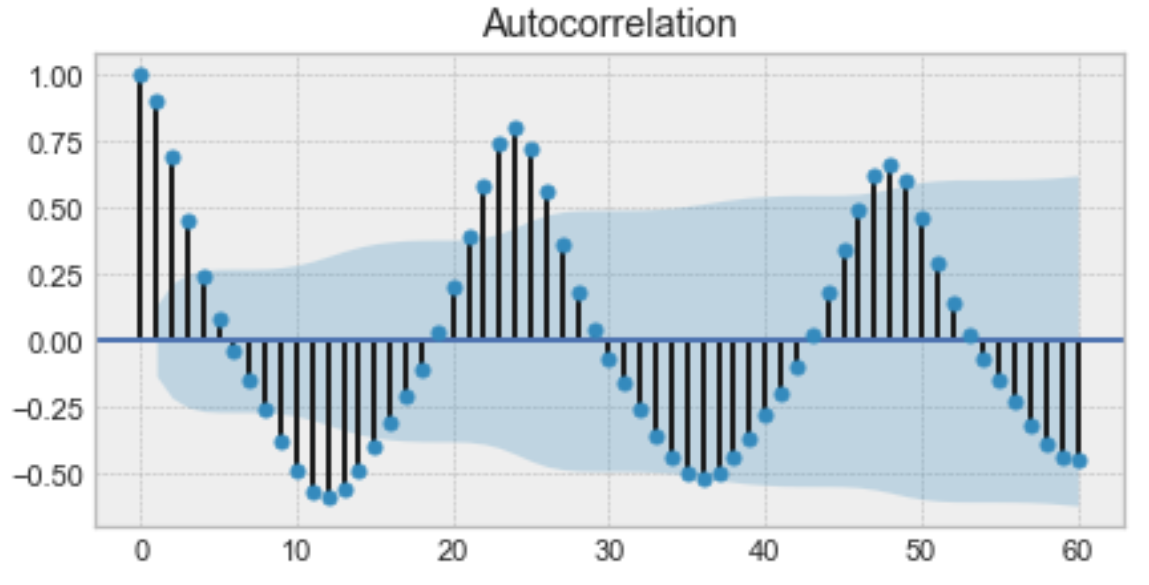
\includegraphics[scale=0.25]{src/sine-wave-autocorrelation.png}
		\item[]	Il y a de l'auto-corrélation cyclique;
		\item[] La 1ère valeur est très semblable à la 24ème, la 12ème à la 36ème, etc. et donc nous allons observer des valeurs très semblables à chaque 24 unité de temps;
		\item[]	De plus, le graphique \textbf{ressemble} évidemment \textbf{à une fonction sinusoïdale};
		\item 	Alors, nous avons un cycle \textbf{saisonnale} pouvant être \textbf{estimé par une fonction sinusoïdale};
		\end{itemize}
%		
	\item[]	\textbf{Fixed effects}
		\begin{itemize}
		\item	\og fixed effects \fg{} représente que la relation est fixe dans le temps;
		\item[]	Pour exemple, on ne s'attend pas à de la neige en juillet;
		\item	On peut représenter beaucoup de patterns avec des fonctions trigonométriques;
		\item	Pour exemple, soit la fonction $g(t) = a \sin (f t + b)$ avec:
		\item[]	$a$: l'\textbf{amplitude}, alias la valeur la plus élevée de la courbe;
		\item[]	$f$: la \textbf{fréquence}, alias le nombre de cycles sur l'intervalle $(0, 2\pi)$
		\item[]	$b$: le \textbf{déphasage};
		\item	Rappel: $\sin(x + y) = \cos(x) \sin(y) + \cos(y) \sin(x)$;
		\item	On réécrit $g(t)$ comme:
		\begin{align*}
			g(t)
				&=	a \sin (f t + b)	\\
				&=	\beta_{1} \sin(ft) + \beta_{2} \cos(ft)	
		\end{align*}
		où
		\begin{align*}
			\beta_{1}	
				&=	a \cos (b)	&
			\beta_{2}	
				&=	a \sin (b)	
		\end{align*}
		\item	Pour une série chrono avec une \textbf{seasonal base} (SB), on défini $f_{i} = \frac{2\pi i}{SB}$ pour l'équation générale:
		\begin{align*}
			S(t)
				&=	a_{i	} \sin (f_{i} t + b_{i})	\\
				&=	\sum_{i = 1}^{m} \{ \beta_{1i} \sin(f_{i}t) + \beta_{2i} \cos(f_{i}t)	 \} 
		\end{align*}
		Pour exemple, si le série était des observations mensuelles alors $SB = 12$;
		\item	Par la suite, on défini le modèle de régression linéaire multiple avec $p = 2m$, et $m \le SB/2$, variables explicatives: 
		\begin{align*}
			y_{t}
				&=	\beta_{0} + S_t + \varepsilon_{t}	\\
				&=	\beta_{0} + \sum_{i = 1}^{m} \{ \beta_{1i} \sin(f_{i}t) + \beta_{2i} \cos(f_{i}t)	 \} + \varepsilon_{t} 
		\end{align*}
		\end{itemize}
	\item[]	\textbf{Autoregressive seasonal models}
		\begin{itemize}
		\item	Le même concept d'avoir les \textit{lagged} variables réponses ($y_{t - 1}$) comme variable explicative peut être appliqué au modèles avec saisonnalité;
		\item	Nous avons donc le \textbf{Seasonal Autoregressive model of \textcolor{burntorange}{Order P}}, SAR(\textcolor{burntorange}{P}), défini comme:
		\begin{align*}
			y_{t}
				&=	\beta_{0} + \beta_{\textcolor{burntorange}{1}}y_{t - SB} + \beta_{\textcolor{burntorange}{2}} y_{t - \textcolor{burntorange}{2}SB} + \dots + \beta_{\textcolor{burntorange}{P}} y_{t - \textcolor{burntorange}{P} SB} + \varepsilon_{t}
		\end{align*}
		\item[]	Pour exemple, si $SB = 12$ alors SAR(\textcolor{burntorange}{1}) est défini comme étant $y_{t} = \beta_{0} + \beta_{\textcolor{burntorange}{1}}y_{t - 12} + \varepsilon_{t}$;
		\item	Chaque terme est donc fonction des P termes précédents;
		\end{itemize}
	\item[]	\textbf{Seasonal exponential smoothing}
		\begin{itemize}
		\item	Holt à généralisé le double exponential smoothing avec 2 smoothing parameters $w_{2}$ et $w_{1}$;
		\item[]	Ce faisant le niveau (intercepte) $\beta_{0}$ et la trend (tendance) $\beta_{1}$ n'ont pas besoin d'avoir le même smoothing parameter;
		\item	L'estimation des paramètres est:
			\begin{align*}
			b_{0, t}	
			&=	(1 - w_{1}) y_{t} + w_{1} (b_{0, t - 1} + b_{1, t - 1})	\\
			b_{1, t}	
			&=	(1 - w_{2}) (b_{0, t} - b_{0, t - 1}) + w_{2} b_{1, t - 1}	
			\end{align*}
		\item	La prévision du modèle avec tendance linéaire $y_{t} = \beta_{0} + \beta_{1}t + \varepsilon_{t}$ est donc la même qu'avec le double exponential smoothing $\hat{y}_{T + l} = b_{0, T} + b_{1, T} l$;
		\item	Par la suite, Winters à généralisé la procédure pour y inclure des \textit{tendances saisonnales};
		\item	Le résultat est le \textbf{Holt-Winters seasonal additive model}:
			\begin{align*}
			y_{t} 
			&= 	\beta_{0} + \beta_{1}t + S_{t} + \varepsilon_{t}
			\end{align*}		
		\item[]	où $S_{t} = S_{t - SB}$ et $S_{1} = S_{2} = \dots = S_{SB} = 0$;
		\item	Le nouveau modèle emploi \textbf{trois smoothing parameters}:		
			\begin{enumerate}
			\item[$w_{1}$]: level;
			\item[$w_{2}$]: trend;
			\item[$w_{3}$]: seasonality;
			\end{enumerate}
		\item	Les estimations des paramètres sont donc:
			\begin{align*}
			b_{0, t}	
			&=	(1 - w_{1}) (y_{t} - \hat{S}_{t - SB}) + w_{1} (b_{0, t - 1} +  b_{1, t - 1})	\\
			b_{1, t}	
			&=	(1 - w_{2}) (b_{0, t} - b_{0, t - 1}) + w_{2} b_{1, t - 1}	\\
			\hat{S}_{t}	
			&=	(1 - w_{3}) (y_{t} - b_{0, t}) + w_{3} \hat{S}_{t - SB}	
			\end{align*}
		\item	Les prévisions:
			\begin{align*}
			\hat{y}_{T + l}
			&=	b_{0, T} + b_{1, T} l + \hat{S}_{T}(l)
			\end{align*}		
		\item[]	où $\hat{S}_{T}(l) = \hat{S}_{T + l}$ pour $l = 1, \dots, SB$, $\hat{S}_{T}(l) = \hat{S}_{T + l - SB}$ pour $l = SB + 1, \dots, 2SB$, etc.;
		\item[]	Pour exemple, si $SB = 12$ alors $\hat{S}_{16} \Leftrightarrow \hat{S}_{4}(12) = \hat{S}_{4}$;	
		\end{itemize}
%%%		
	\item	\textbf{Unit root tests}
	\item[]	\textbf{Contexte}
		\begin{itemize}
		\item	Les \textit{unit root tests} servent à tester si une série est stationnaire ou pas;
		\item	Ce faisant, une série est non-stationnaire lorsqu'elle \textit{possède} une unit root;
		\item	Le test de Dickey-Fuller en est un exemple;
		\item	Le test sert à déterminer si la tendance d'une série chronologique est linéaire, auto-régressive, ou une marche aléatoire;	
		\item	Pour ce faire, on établit le système de régression:
			\begin{equation*}
			y_{t} - y_{t - 1}	
			=	\beta_{0} + (\phi - 1) y_{t - 1} + \beta_{1} t + \varepsilon_{t}
			\end{equation*}
		\item[]	On observe que: 
			\begin{enumerate}
			\item	Si $\phi = 1$, la série est une marche aléatoire avec $y_{t} = \beta_{0} + \beta_{1} t + y_{t - 1} + \varepsilon_{t} $;
			\item	Si $\phi < 1$ et que $\beta_{1} = 0$, la série est une auto-régression AR(1) avec $y_{t} = \beta_{0} + \phi y_{t - 1} + \varepsilon_{t}$ 
			\item[]	\textit{(Le paramètre $\phi$ est le paramètre de tendance habituellement écrit comme $\beta_{1}$)};
			\item	Si $\phi = 0$, la série est une tendance linéaire avec $y_{t} = \beta_{0} + \beta_{1} t + \varepsilon_{t} $;
			\end{enumerate}
		\end{itemize}
	\item[]	\textbf{Test} Dickey-Fuller et statistique $t$ :
		\begin{itemize}
		\item[]	Si la série est une marche aléatoire, $\phi = 1$, elle est \textit{non-stationnaire};
		\item	On cherche donc à faire un test très semblable au \textit{test d'auto-corrélation} du chapitre 20 pour \textbf{tester la stationnarité} de la série:
		\setlength{\mathindent}{-2cm}
			\begin{align*}
			\mathcal{H}_{0} &:	\phi = 1, \ \text{le modèle est non-stationnaire (marche aléatoire)}	\\
			\mathcal{H}_{1} &:	\phi < 1, \ \text{le modèle est stationnaire}	
			\end{align*}
		\setlength{\mathindent}{1cm}
		\item	Cependant, puisque sous l'hypothèse nulle la série est une marche aléatoire, $t_{ddl}$ \textit{ne suit \textbf{pas} la distribution $t$ habituelle} ($t_{ddl} \not\sim t$) mais plutôt une distribution spéciale;
		\end{itemize}
%		
	\item[]	Test \textbf{Dickey-Fuller} :
		\begin{itemize}
		\item	Le test \textit{Dickey-Fuller} est donc conçu pour ce test d'hypothèse;
		\item[\textbf{Note}]: Les valeurs critiques compilées par Dickey-Fuller sont plus élevées que le test habituel;
		\item[]	Ce faisant, il est plus difficile de rejeter l'hypothèse d'une marche aléatoire et est donc typique d'utiliser un seuil de 10\% au lieu de 5\% pour compenser;		
		\item	Le test pose que les erreurs $\varepsilon_{t}$ ne sont pas auto-corrélées alors que le \textit{test \textbf{augmenté} de Dickey-Fuller} le permet:
			\begin{equation*}
			y_{t} - y_{t - 1}	
			=	\beta_{0} + (\phi - 1) y_{t - 1} + \beta_{1} t + \sum_{j = 1}^{p} \phi_{j} (y_{t - j} - y_{t - j - 1}) + \varepsilon_{t}
			\end{equation*}
		\item[]	Le test augmenté inclut les lagged variables dans le modèle de régression;
		\item[]	Du fait, c'est la même idée que le généralisation du ARCH par le GARCH ci-dessous;
		\item	Typiquement, pour déterminer le nombre $p$ de variables lagged, le test est répété pour plusieurs valeurs possibles;
		\end{itemize}
%%%		
	\item	\textbf{Modèles de volatilité}
	\item[]	Description du modèle \textbf{ARCH}
		\begin{itemize}
		\item	C'est le \textbf{Auto Regressive Changing Heteroscedasticity}, ou \textit{Auto Regressive \textbf{Conditional} Heteroscedasticity}, model d'ordre p---ARCH(p):
		\item	\textit{Heteroscedasticité} veut juste dire que la volatilité, ou variance, n'est \textbf{pas constante} dans le temps;
		\item[]	En observant la graphique du vidéo sur ARCH de ritvikmath, on voit que la volatilité \textbf{change} dans le temps;
		\item[] Annuellement, il y a une période de temps pour laquelle les résidus sont très volatiles, mais que pour le reste de l'année elle est relativement stable;
		\item	C'est-à-dire, la volatilité est \textbf{conditionnelle} à le moment dans le temps où nous sommes;
		\item[]	L'erreur à un moment dépend de l'erreur au moment précédent et donc nous avons un  modèle \textbf{auto-régressif};
		\end{itemize}
	\item[]	\textbf{Variance} du modèle ARCH
		\begin{itemize}
		\item	La volatilité, ou plutôt variance $\text{Var}(\varepsilon_{t}) = \sigma^{2}_{t}$, d'aujourd'hui est fonction de celle du passé;
		\item	Pour un modèle d'ordre \textcolor{lava}{1}, ARCH(\textcolor{lava}{1}), on obtient:
			\begin{align*}
			\sigma^{2}_{t}	&=	w + \gamma_{\textcolor{lava}{1}} \varepsilon_{t - \textcolor{lava}{1}}^{2}
			\end{align*}
		\item[]	On peut voir la \textbf{volatilité à long-terme} $w$ un peu comme une volatilité \og \textit{moyenne} \fg{} à l'entour de laquelle les erreurs se situent;
		\item[]	Donc, $\gamma_{1}$ est l'importance, ou \textbf{poids}, à accorder à l'erreur de la période précédente;
		\item	Plus généralement, la variance conditionnelle d'un modèle d'ordre \textcolor{lava}{P} AR\textcolor{lava}{CH}(\textcolor{lava}{P}) est:
			\begin{align*}
			\sigma^{2}_{t}	&=	w + \sum_{j = 1}^{\textcolor{lava}{p}} \gamma_{j} \varepsilon_{t - j}^{2}
			\end{align*}
		\item	Et la variance inconditionnelle: 
			\begin{align*}
			\text{Var}(\varepsilon_{t})	
			&=	\frac{w}{1 - \sum \gamma_{j}}
			\end{align*}
		\item	Donc, plus P est large plus on capture des effets à plus long-terme;
		\item	Quelques conditions:
			\begin{align*}
			w &> 0	&	
			\gamma_{j} &\ge 0	&
			\sum_{j = 1}^{p} \gamma_{j} &< 1
			\end{align*}
		\end{itemize}
	\item[]	\textbf{Généralisation} du modèle ARCH
		\begin{itemize}
		\item	Nous avons le \textbf{\textit{Generalized} Auto Regressive Changing Heteroscedasticity} model d'ordre P textcolor{teal}{G}ARCH(p, \textcolor{teal}{q});
		\item	Le GARCH complément le ARCH de la même façon que le modèle de moving average complément le modèle auto-régressif;
		\item	Le \textcolor{teal}{G}AR\textcolor{lava}{CH}(\textcolor{lava}{p}, \textcolor{teal}{q}) inclut une dépendance sur les \textcolor{teal}{q} dernières variances:
			\begin{align*}
			\sigma^{2}_{t}	&=	w + \sum_{j = 1}^{\textcolor{lava}{p}} \gamma_{j} \varepsilon_{t - j}^{2} + \sum_{i = 1}^{\textcolor{teal}{q}} \delta_{i} \textcolor{teal}{\sigma^{2}_{t - i}}
			\end{align*}
		\item	Quelques conditions:
			\begin{align*}
			w &> 0	&	
			\delta_{i}	&\ge 0	&
			\gamma_{i} &\ge 0	&
			\sum_{j = 1}^{p} \gamma_{j} + \sum_{i = 1}^{q} \delta_{i} &< 1
			\end{align*}
		\end{itemize}
	\item[]	\textbf{Stationnarité} et \textbf{variance \textit{conditionnelle}}
		\begin{itemize}
		\item	Un modèle GARCH est stationnaire et a comme variance \textbf{in}conditionnelle:
			\begin{align*}
			\text{Var}(\varepsilon_{t})	
			&=	\frac{w}{1 - \sum \gamma_{j} - \sum \delta_{i}}
			\end{align*}
		\end{itemize}
\end{enumerate}

\textbf{Note sur les exercices:} 
\begin{enumerate}
	\item	Pour smoothing exponentiel, questions sont de récursivement calculer une prévision;
	\item	Pour le Holt-Winters model, calculer récursivement une prévision / les paramètres;
	\item	Pour le ARCH/GARCH ce serait quelque-chose avec les variances (style \# 15);
\end{enumerate}
\end{CHPT_SUMM}

\begin{FORMULA_SUMM}{Formules chapitre 21}
\begin{multicols*}{2}
Moving average smoothing

\begin{minipage}[ht]{0.5\linewidth}
\setlength{\mathindent}{-1cm}
\begin{align*}
	\hat{s}_{t}
		&=	\frac{y_{t - (k - 1)} + y_{t - (k - 2)} + \dots + y_{t}}{k}	\\
		&=	\hat{s}_{t - 1} + \frac{y_{t} - y_{t - k}}{k}	
\end{align*}
\setlength{\mathindent}{1cm}
\end{minipage}
\setlength{\mathindent}{-1cm}
\begin{align*}
	b_{1, T}	
		&=	\frac{2(\hat{s}_{t}^{(1)} - \hat{s}_{t}^{(2)})}{k - 1}	\\
	\hat{y}_{T + l}
		&=	\hat{s}_{t} + b_{1, T} l	\\
	\hat{s}_{t}^{(2)}	
		&=	\frac{\hat{s}_{t}^{(1)} + \dots + \hat{s}_{t - (k - 1)}^{(1)}}{k}	
\end{align*}
\setlength{\mathindent}{1cm}

\vfill\null
\

\begin{minipage}[ht]{0.5\linewidth}
Exponential smoothing
\setlength{\mathindent}{-1cm}
\begin{align*}
	\hat{s}_{t}
		&=	\frac{y_{t} + w y_{t - 1} + w^{2} y_{t - 2} + \dots + w^{t} y_{0}}{1/(1 - w)}		\\
		&=	w \hat{s}_{t - 1} + (1 - w) y_{t}	
\end{align*}
\setlength{\mathindent}{1cm}
\end{minipage}
\setlength{\mathindent}{-1cm}
\begin{align*}
	b_{1, T}	
		&=	\frac{(1 - w)}{w}\left(\hat{s}_{t}^{(1)} - \hat{s}_{t}^{(2)}\right)	\\
	\hat{y}_{T + l}
		&=	b_{0, T} + b_{1, T} l	\\
	\varepsilon_{t}
		&=	y_{t} - \hat{s}_{t - 1}	\\
	SS(w)
		&=	\sum_{t = 1}^{T}(y_{t} - \hat{s}_{t - 1})^{2}, \hat{s}_{0} = y_{0}	
\end{align*}
\setlength{\mathindent}{1cm}
\end{multicols*}

Seasonal models
Fixed effects
\begin{align*}
	y_{t}
		&=	\beta_{0} + S_t + \varepsilon_{t}	\\
		&=	\beta_{0} + \sum_{i = 1}^{m} \{ \beta_{1i} \sin(f_{i}t) + \beta_{2i} \cos(f_{i}t)	 \} + \varepsilon_{t} 
\end{align*}

SAR\textcolor{burntorange}{P}
\begin{align*}
	y_{t}
	&=	\beta_{0} + \beta_{\textcolor{burntorange}{1}}y_{t - SB} + \beta_{\textcolor{burntorange}{2}} y_{t - \textcolor{burntorange}{2}SB} + \dots + \beta_{\textcolor{burntorange}{P}} y_{t - \textcolor{burntorange}{P} SB} + \varepsilon_{t}	\\
\end{align*}

Holt-Winters seasonal additive model
\begin{align*}
	y_{t} 
	&= 	\beta_{0} + \beta_{1}t + S_{t} + \varepsilon_{t}
\end{align*}
\begin{align*}
	b_{0, t}	
	&=	(1 - w_{1}) (y_{t} - \hat{S}_{t - SB}) + w_{1} (b_{0, t - 1} +  b_{1, t - 1})	\\
	b_{1, t}	
	&=	(1 - w_{2}) (b_{0, t} - b_{0, t - 1}) + w_{2} b_{1, t - 1}	\\
	\hat{S}_{t}	
	&=	(1 - w_{3}) (y_{t} - b_{0, t}) + w_{3} \hat{S}_{t - SB}	
\end{align*}
\begin{align*}
	\hat{y}_{T + l}
	&=	b_{0, T} + b_{1, T} l + \hat{S}_{T}(l)
\end{align*}

\textbf{Unit root test}

\textbf{ARCH}

\textbf{GARCH}
\end{FORMULA_SUMM}


\subsection{Notes sur les vidéos YouTube}

\begin{YTB_SUMM}{\href{https://www.youtube.com/watch?v=-gmlyRRscXo}{Ben Lambert: Time series vs cross sectional data}}
Le vidéo est utile pour commencer à conceptualiser la différence en approche des données auxquelles nous sommes habituées (\textit{cross-sectional data}) des données de séries chronologiques.

Pour ce, et les prochains vidéos de Ben Lambert, $u_{t} = \varepsilon_{t}$.

\begin{minipage}{0.2\linewidth}
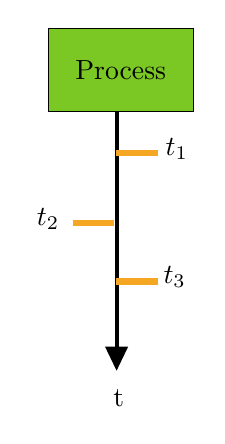
\begin{tikzpicture}[x=0.75pt,y=0.75pt,yscale=-1,xscale=1]
%uncomment if require: \path (0,300); %set diagram left start at 0, and has height of 300

%Shape: Rectangle [id:dp45341716963014833] 
\draw  [fill={rgb, 255:red, 109; green, 194; blue, 12 }  ,fill opacity=0.9 ] (74,51) -- (144,51) -- (144,91) -- (74,91) -- cycle ;
%Straight Lines [id:da3471781120754416] 
\draw [line width=1.5]    (107,91) -- (107,212) ;
\draw [shift={(107,216)}, rotate = 270] [fill={rgb, 255:red, 0; green, 0; blue, 0 }  ][line width=0.08]  [draw opacity=0] (11.61,-5.58) -- (0,0) -- (11.61,5.58) -- cycle    ;

%Straight Lines [id:da24464797721586562] 
\draw [color={rgb, 255:red, 245; green, 166; blue, 35 }  ,draw opacity=1 ][line width=2.25]    (85.83,145) -- (105.83,145) ;

%Straight Lines [id:da022853384994410142] 
\draw [color={rgb, 255:red, 245; green, 166; blue, 35 }  ,draw opacity=1 ][line width=2.25]    (106.83,173) -- (126.83,173) ;

%Straight Lines [id:da31936638200020173] 
\draw [color={rgb, 255:red, 245; green, 166; blue, 35 }  ,draw opacity=1 ][line width=2.25]    (106.83,111) -- (126.83,111) ;

% Text Node
\draw (108,229) node   [align=left] {t};
% Text Node
\draw (136,109) node   [align=left] {$\displaystyle t_{1}$};
% Text Node
\draw (74,143) node   [align=left] {$\displaystyle t_{2}$};
% Text Node
\draw (135,171) node   [align=left] {$\displaystyle t_{3}$};
% Text Node
\draw (109,71) node   [align=left] {Process};
\end{tikzpicture}
\end{minipage}
\begin{minipage}{0.8\linewidth}
\begin{itemize}
	\item	With cross-sectional data, we can think of the data as a population from which we take random samples;
	\item	With time series data however, it is not so simple;
	\item	Time series data is actually a \textbf{process} that evolves with time;
	\item	Thereby, when we see observations of the process, we're really sampling the process at different time (for example, $t_{1}, t_{2}, t_{3}, \dots$);
	\item	The \og \textit{population} \fg{} is actually all the observations for all the possible periods of in time but that is quite untangible;
	\item	Thus, we have more specific conditions than normal cross-sectional data with regards to independance, etc.
\end{itemize}   
\end{minipage}
\end{YTB_SUMM}

\begin{YTB_SUMM}{\href{https://www.youtube.com/watch?v=bWo_ka37szw&list=PLvo9ZnEQG5oXC-cg8ecXr6SJZWprEL1UC&index=3}{Ben Lambert: Time series Gauss Markov conditions}}
Rappel: $u_{t} = \varepsilon_{t}$.

On a appris en modèle à propos des 4 hypothèses pour un LM et que la 4ème n'était pas \textit{vraiment} nécessaire. En réalité, les 3 premières sont le théorème \textbf{Gauss-Markov} qui prouve qu'un estimateur est le \textbf{Best Linear Unbiased Estimator \textit{(BLUE)}}. 

Il est important de faire cette distinction pour les séries chronologiques puisque les conditions sont légèrement différentes d'une façon importante. Entres autres, puisque les données ne sont pas indépendantes nous avons plusieurs conditions pour la corrélation / colinéarité. Ce vidéo explique le tout.
\begin{enumerate}
	\item[]	The first three prove the estimator is unbiased.
	\item	Linearity: $Y_{t} = \alpha + \beta_{1} x_{1t} + \beta_{2} x_{2t} + \varepsilon_{t}$.
	\item[]	Thus we have $p = 2$.
	\item	Nul expectation
	\begin{align*}
		\text{E}[\varepsilon_{t} | x_{pk}] &=	0	&
		&\text{vs}	&
		\text{E}[\varepsilon_{i} | x_{pi}] &=	0
	\end{align*}
	\begin{itemize}
		\item	In linear regression, we only need the $i^{\text{th}}$ observation's expected value to be 0 for all $p$ parameters;
		\item	In time series however, we need the expected value of the observation over \textbf{all possible time intervals} $k$ to be 0. 
	\end{itemize}
	\item	No perfect colinearity (i.e. no multicolinearity)
	\item	Homoscedasticity
	\item[]	The same idea holds for the variance.
	\begin{align*}
		\text{Var}(\varepsilon_{t} | x_{pk}) &= \sigma^{2}	&
		&\text{vs}	&
		\text{Var}(\varepsilon_{i} | x_{pi}) &= \sigma^{2}
	\end{align*}
	\item	No serial correlation: $\text{cov}(\varepsilon_{t}, \varepsilon_{s} | x_{pk}) = 0$
	\item[]	The same idea holds again for the correlation.
\end{enumerate}
With these conditions, we prove the OLS is BLUE.
\end{YTB_SUMM}

\begin{YTB_SUMM}{\href{https://www.youtube.com/watch?v=LgIOgb-6mYA&list=PLvo9ZnEQG5oXC-cg8ecXr6SJZWprEL1UC&index=3}{Ben Lambert: Strict exogeneity}}
\begin{itemize}
	\item	By including the previous value in the model, we remove the problem of the monetary policy at time 2 being dependant on the monetary police 2 units of time ago;
	\item	It’s a \textbf{lagged effect} because the dependant variable depends on itself;
	\item	Also, adding the lagged variable makes the model \textit{dynamic};
	\item	However, what if the dependant variable, say sales, is actually dependant on a \textbf{function} of the sales at a previous time and not just the amount of sales themselves?
	\item	Well this is what we can't easily model and as such the model would have \textbf{weak exogeneity} and \textbf{NOT \textit{strict} exoogenity};
\end{itemize}
\end{YTB_SUMM}

\begin{YTB_SUMM}{\href{https://www.youtube.com/watch?v=a7_3qX67e7c&list=PLvo9ZnEQG5oXC-cg8ecXr6SJZWprEL1UC&index=4}{Ben Lambert: Strict exogeneity assumption - intuition}}
\begin{itemize}
	\item	Because sales is, obviously, highly correlated with itself then of course advertising will also seem very correlated;
	\item	The impact is that the OLS estimate of the parameter will be > the true parameter;
\end{itemize}
\end{YTB_SUMM}

\begin{YTB_SUMM}{\href{https://www.youtube.com/watch?v=5-2C4eO4cPQ&list=PLvcbYUQ5t0UHOLnBzl46_Q6QKtFgfMGc3&index=5}{ritvikmath: Time Series Talk : Autoregressive model}}
\begin{itemize}
	\item	Auto\textbf{regressive}: means regression
	\item	\textbf{Auto}regressive: means predict something based on past values of that same thing
	\item	\textbf{Emphasis} on how \textbf{natural} it is to want to \textit{predict the value} of something based on \textit{what it was} in the past;
	\item[]	For example, price of an item, number of houses sold per month, etc.;
	\item[]	Then you can \textbf{identify patterns} on how that something evolves over time;
	\item	Want to identify \textbf{which lags}, i.e. which \textit{past values}, are the most \textbf{important};
	\item[]	We don't want all the past values or model would be overly complex;
	\item	This is where the importance of seasonal patterns come into play;
	\item[]	For example, maybe the value 12 months ago is much more important than few previous months;
	\item	This is thus evaluated with the autocorrelation function (ACF);
	\item[]	We'd only want to include the lags with an ACF value above a certain band;
	\item	\textbf{We only want the lags whose direct effects are high in magnitude}	
	\item	Example from video:
	
	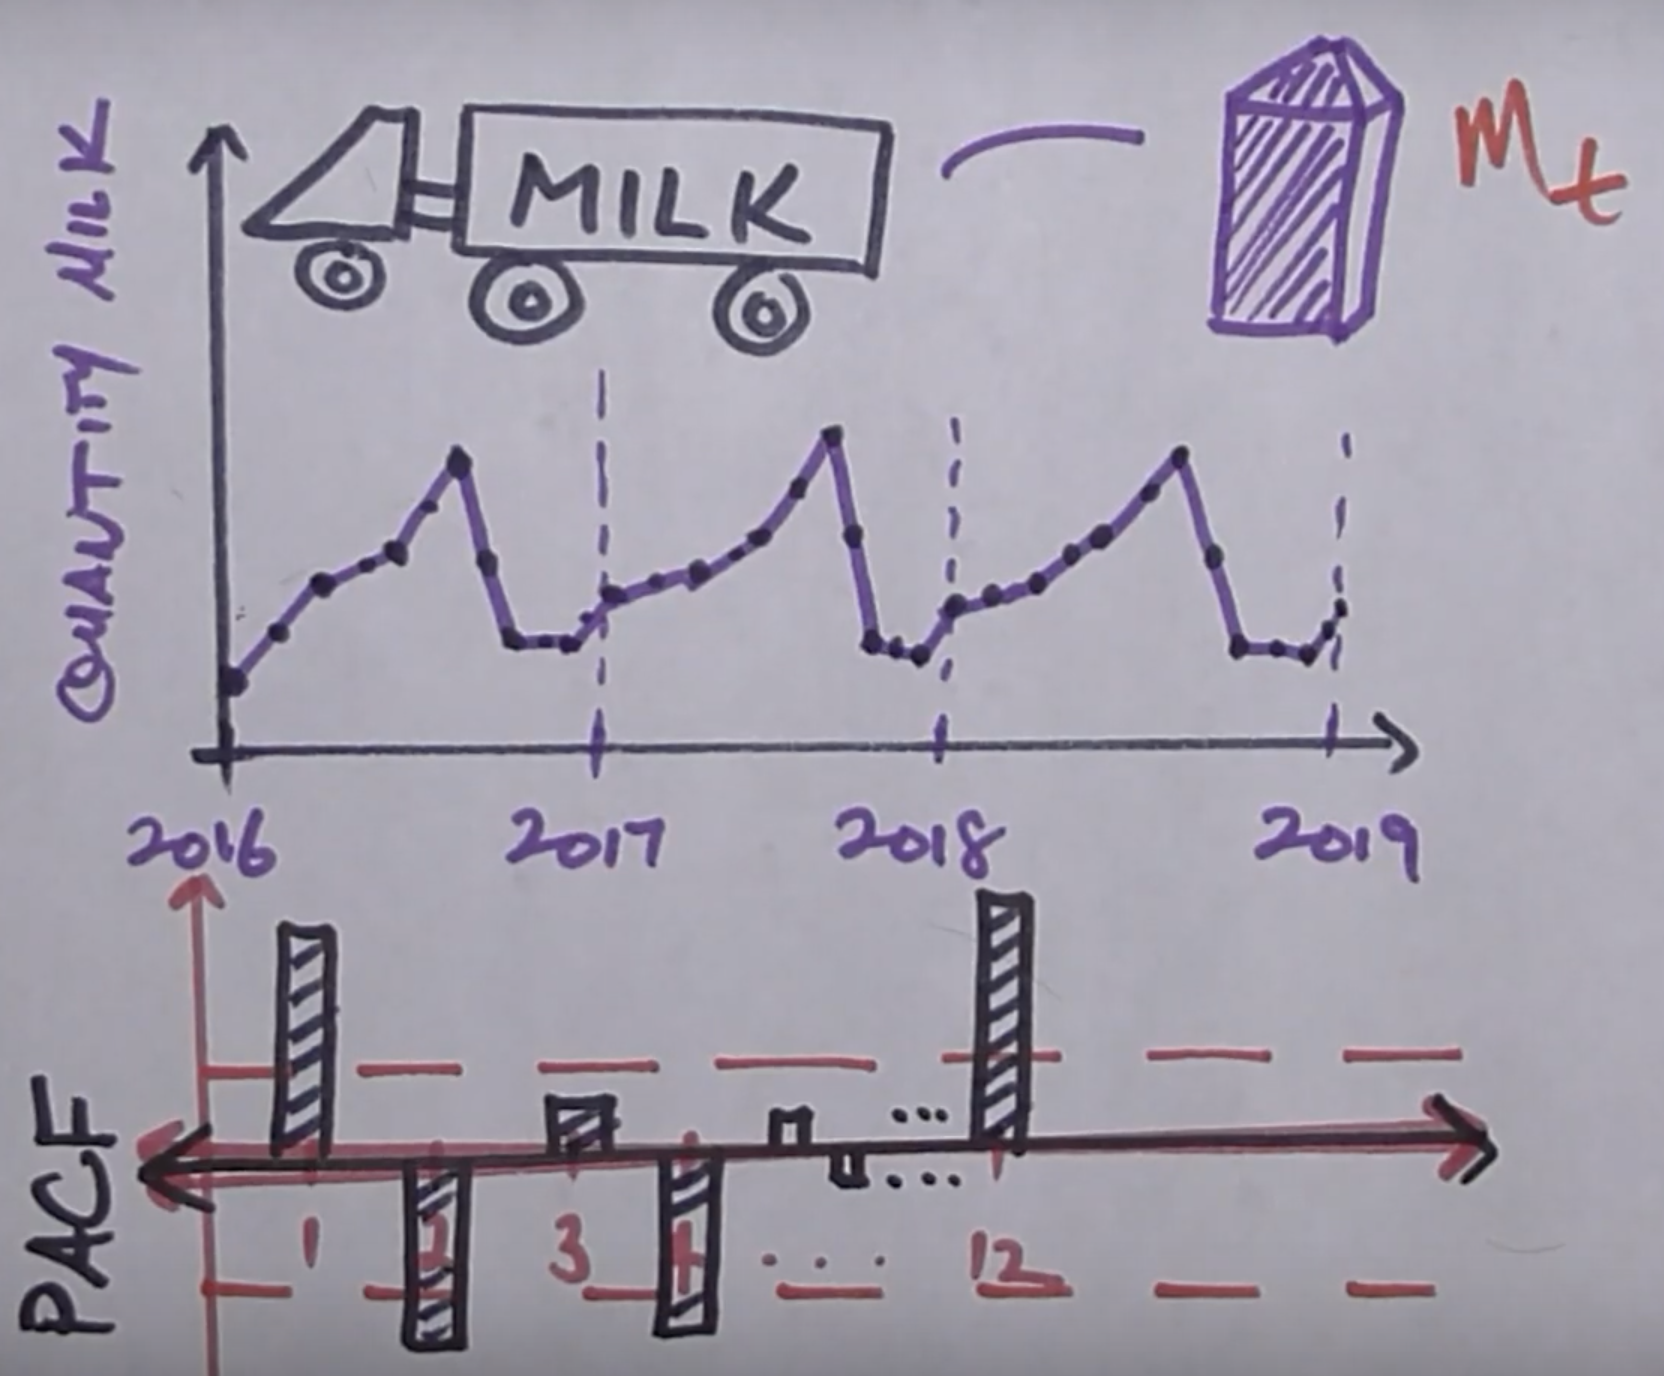
\includegraphics[scale=0.2]{src/ritvikmath-lags-pcf.png}
\end{itemize}
\end{YTB_SUMM}

\begin{YTB_SUMM}{\href{https://www.youtube.com/watch?v=voryLhxiPzE&list=PLvcbYUQ5t0UHOLnBzl46_Q6QKtFgfMGc3&index=6}{ritvikmath: Time Series Talk : Moving Average Model}}
Food equation: $\hat{f}_{t} = \mu + \phi_{1} \varepsilon_{t - 1} = 10 + 0.5 \varepsilon_{t - 1} $
\begin{itemize}
	\item	First parameter is the baseline;
	\item[]	Ceteris paribus, you would bring 10 cupcakes to the party so $\mu = 10$;
	\item	Professor's crazy and every month he's gonna say you brought the wrong number of cupcakes by a certain amount $\varepsilon_{t}$;
	\item[]	This amount is normally distributed with an average of $\mu_{\varepsilon}$ of cupcakes which is usually 0 and a variability of the wrong number of cupcakes $\sigma_{\varepsilon}$ that we'll say is 1;
	\item	$\varepsilon \sim \mathcal{N}(\mu_{\varepsilon} = 0, \sigma_{\varepsilon} = 1)$
	\item	Since we know he's a little crazy, want to take into account the error into the amount of cupcakes we bring each month;
	\item	Logically, each month we will therefore look at how close we were to bringing the right amount of cupcakes last month and take that into account;
	\item	The amount of consideration for last month's error is $\phi_{1}$ which we set to $0.5$;
	\item[]	Thereby, I'm always gonna bring 10 cupcakes but will adjust by whatever the professor said was my error last time;
	\item[]	The first month, I'd bring 10;
	\item[]	Last month I brought 10 and only needed 8 so my error was 2;
	\item[]	This month I'll bring $10 + 0.5 * (-2) = 9$;
	\item[]	The professor says I was off by one and should've brought 10;
	\item[]	The following month I'll bring $10 + 0.5 (1) = 10.5$ (pretend can bring fractionnal amount of cupcakes);
	
	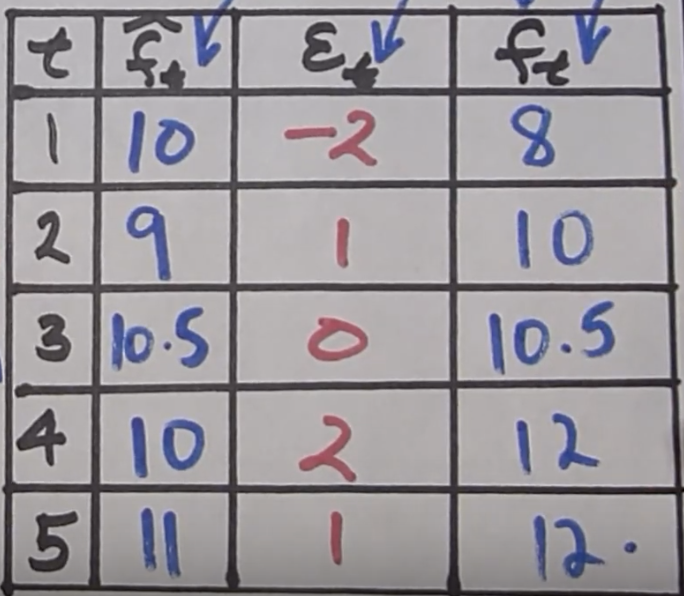
\includegraphics[scale=0.4]{src/ritvikmath-MA-table.png}
	\item	So we have our average, 10, and we move around it always being centered at 10 -> \textbf{\textit{moving} average model};
	\item	This is the MA(1) model because we only take into account last month's error;
	\item	The real amount of cupcakes would therefore be $f_{t} = \mu + \phi_{1} \varepsilon_{t - 1} + \textcolor{burntorange}{\varepsilon_{t}}$;
	\item[]	i.e., we take into account \textit{this month's error};
\end{itemize}
\end{YTB_SUMM}

\begin{YTB_SUMM}{\href{https://www.youtube.com/watch?v=HhvTlaN06AM&list=PLvcbYUQ5t0UHOLnBzl46_Q6QKtFgfMGc3&index=8}{ritvikmath: Time Series Talk: ARMA Model}}
Lightbulb manufacturer. Challenge is: how many lightbulbs ($k_{t}$) to manufacture?
\begin{itemize}
	\item	We use the \textbf{Auto Regressive Moving Average} \textcolor{amethyst}{AR}\textcolor{burntorange}{MA}(1, 1) model: 
	\begin{equation*}
		l_{t} = \beta_{0} + \textcolor{amethyst}{\beta_{1} l_{t - 1}} + \textcolor{burntorange}{\phi_{1} \varepsilon_{t - 1}} + \varepsilon_{t}
	\end{equation*}
	\item[]	The \textcolor{amethyst}{autoregressive bit} is the number of lightbulbs need to create last month;
	\item[]	The \textcolor{burntorange}{moving average bit} is the error from the previous time period;
	\item	Anything \og hat \fg{} is the forecast in time series;
	\begin{equation*}
		\hat{l}_{t} = \beta_{0} + \textcolor{amethyst}{\beta_{1} l_{t - 1}} + \textcolor{burntorange}{\phi_{1} \varepsilon_{t - 1}}
	\end{equation*}
	\item	Rule of thumb to identify the order of the ARMA model is the correlation functions
	\item[]	ACF helps identify the MA order because it measures direct effects;
	\item[]	PACF helps identify the AR order because it measures the moving average bit;
\end{itemize}
\end{YTB_SUMM}

\begin{YTB_SUMM}{\href{https://www.youtube.com/watch?v=3UmyHed0iYE&list=PLvcbYUQ5t0UHOLnBzl46_Q6QKtFgfMGc3&index=9}{ritvikmath: Time Series Talk: ARIMA Model}}
\begin{itemize}
	\item	Context is salesman of anchors;
	\item[]	The number of anchors sold is $a_{t}$;
	\item[]	We see the time series doesn't have a constant mean and thus is not stationnary;
	
	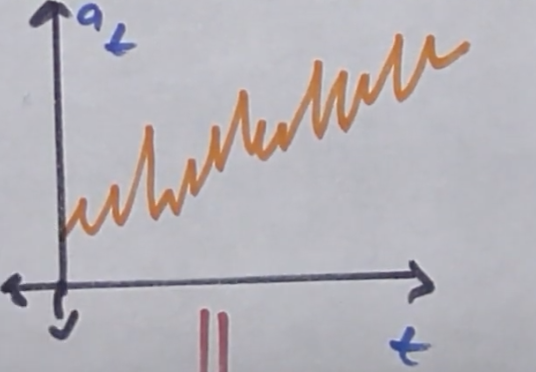
\includegraphics[scale=0.4]{src/ritvikmath-anchors-plot.png}
	\item[]	Therefore, we can't use the straight AR, MA, or ARMA models;
	\item	However, if we could \textbf{eliminate the trend} we could probably use it;
	\item[]	Enter, the ARIMA model;
	\item[]	When things look stationnary except for a trend, a \textbf{moving mean};
	\item	\textbf{Auto Regressive \textit{Integrated} Moving Average} (ARIMA) model;
	\item[]	Integrated means that \textbf{instead} of predicting the time series itself, we \textbf{predict \textit{differences} of the time series} between 2 times;
	
	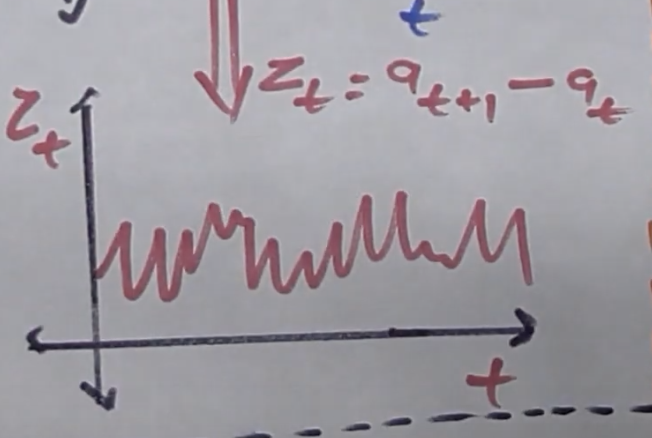
\includegraphics[scale=0.4]{src/ritvikmath-anchors-plot-diff.png}
	\item	If we take the diference between a linear function from one time stamp to the next, we expect linearity;
	\item[]	So, we expect the same behaviour from our time series;
	\item[]	We expect it to hover around a constant and that's what we see with the transformation;
\end{itemize}
\begin{itemize}
	\item	\textcolor{amethyst}{AR}\textcolor{teal}{I}\textcolor{burntorange}{MA}(\textcolor{amethyst}{p}, \textcolor{teal}{d}, \textcolor{burntorange}{q})
	\item[]	\textcolor{amethyst}{p} and \textcolor{burntorange}{q} are both orbiters but \textcolor{amethyst}{p} for the \textcolor{amethyst}{AR} part and \textcolor{burntorange}{q} for the \textcolor{burntorange}{MA} part;
	\item[]	\textcolor{teal}{d} is the orbiter for the \textcolor{teal}{Integrated (I)} part;
	\item	The second difference, \textcolor{teal}{d = 2}, would be creating a new series of the differences of the series of differences of the original series;
	\item[]	However, once is usually sufficient;
	\item	The integrated bit is take care of by $\textcolor{teal}{z_{t}}$ being a difference:
	\begin{equation*}
		\textcolor{teal}{z_{t}}	=	\textcolor{amethyst}{\phi_{1}} z_{t - 1} + \textcolor{burntorange}{\theta_{1}} \varepsilon_{t - 1}
	\end{equation*}	
	\item	To recover the original value, $a_{k}$, 
	\item	Alot of time series is just how complicated can we make this acronym
\end{itemize}
\end{YTB_SUMM}

\begin{YTB_SUMM}{\href{https://www.youtube.com/watch?v=4hrMdu9CSQs&list=PLvcbYUQ5t0UHOLnBzl46_Q6QKtFgfMGc3&index=10}{ritvikmath: Time Series Talk : What is seasonality?}}
\begin{itemize}	
	\item	Setup: Ice cream vendor;
	\item	\textbf{Seasonality}: Repeating \textbf{predictible} pattern \textbf{within a year}
	
	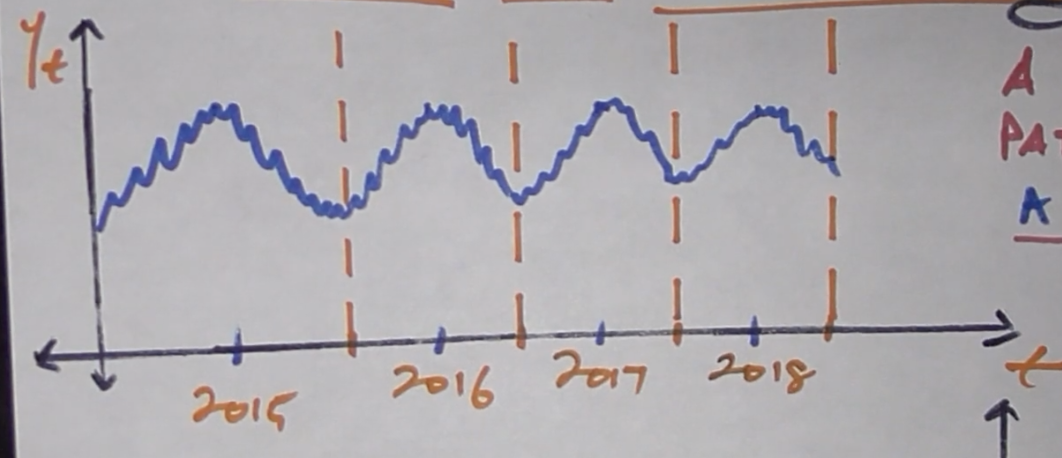
\includegraphics[scale=0.4]{src/ritvikmath-seasonality-plot.png}
	\item	If there's seasonality then it's \textit{not stationnary} so we want to remove it;
	\item[]	Lots of ways to remove it;
	
	\item	\textbf{Cycle}: Repeating pattern over the course of years, and \textbf{aren't predictible}
\end{itemize}
\end{YTB_SUMM}

\begin{YTB_SUMM}{\href{https://www.youtube.com/watch?v=VPNijQ2L3XM}{ritvikmath: Time Series Talk : Lag Operator}}
\begin{enumerate}
	\item	Takes alot of space to write out, for example, an ARMA(3, 3) model:
	\begin{equation*}
	y_{t} = \phi_{1}y_{t - 1} + \phi_{2}y_{t - 2} + \phi_{3}y_{t - 3} + \theta_{1} \varepsilon_{t - 1} + \theta_{2} \varepsilon_{t - 2} + \theta_{3} \varepsilon_{t - 3}
	\end{equation*}
	\item	So, we want to use the \textbf{backshift} or \textbf{lag} operator;
	\item	First, we rewrite the equation:
	\begin{equation*}
	y_{t} - \phi_{1}y_{t - 1} - \phi_{2}y_{t - 2} - \phi_{3}y_{t - 3} = \theta_{1} \varepsilon_{t - 1} + \theta_{2} \varepsilon_{t - 2} + \theta_{3} \varepsilon_{t - 3}
	\end{equation*}
	\item	And then plug in the lag operator $L$ such that $L y_{t} = y_{t - 1}$:
	\begin{equation*}
	1 \ y_{t} - \phi_{1} L y_{t} - \phi_{2} L^{2} y_{t} - \phi_{3} L^{3} y_{t} 
	= 
	\theta_{1} L \varepsilon_{t} + \theta_{2} L^{2} \varepsilon_{t} + \theta_{3} L^{3} \varepsilon_{t}
	\end{equation*}
	\item	Then we factor out the $y_{t}$ and $\varepsilon_{t}$:
	\begin{equation*}
	(1 - \phi_{1} L - \phi_{2} L^{2} - \phi_{3} L^{3}) y_{t} 
	= 
	(\theta_{1} L + \theta_{2} L^{2} + \theta_{3} L^{3}) \varepsilon_{t}
	\end{equation*}
	\item	Then we define the \textbf{lag polynomial}
	\begin{equation*}
	\Phi(L) y_{t} 
	= 
	\Theta(L) \varepsilon_{t}
	\end{equation*}
\end{enumerate}
\end{YTB_SUMM}

\begin{YTB_SUMM}{\href{https://www.youtube.com/watch?v=WjeGUs6mzXg&list=PLvcbYUQ5t0UHOLnBzl46_Q6QKtFgfMGc3&index=2}{ritvikmath: Time Series Talk: Seasonal ARIMA Model}}
\begin{itemize}
	\item	Seasonal ARIMA model;
	\item	\textcolor{ao(english)}{S}\textcolor{amethyst}{AR}\textcolor{teal}{I}\textcolor{burntorange}{MA} $(\textcolor{amethyst}{p}, \textcolor{teal}{d}, \textcolor{burntorange}{q}) (\textcolor{amethyst}{P}, \textcolor{teal}{D}, \textcolor{burntorange}{Q})_{\textcolor{ao(english)}{m}}$
	\item	Backshift operator $B$, aka lag operator, means to back up by one time unit
	\item	For example, $(1, \textcolor{teal}{1}, 1) (1, \textcolor{teal}{1}, 1)_{4}$  implies:
	\begin{equation*}
		\textcolor{amethyst}{(1 - \phi_{1} B)}\textcolor{amethyst}{(1 - \Phi_{1} B^{4})}\textcolor{teal}{(1 - B)}\textcolor{teal}{(1 - B^{4})} y_{t} = \textcolor{burntorange}{(1 + \theta_{1} B)} \textcolor{burntorange}{(1 + \Theta_{1} B^{4})} \varepsilon_{t}
	\end{equation*}
	The powers to the four correspond to the uppercase letters and are the seasonal components;
	\item	$z_{t} = y_{t} - y_{t - 4} = \phi_{1} z_{t - 1} + \Theta_{1} \varepsilon_{t - 4} + \varepsilon_{t}$
\end{itemize}
\end{YTB_SUMM}	

\begin{YTB_SUMM}{\href{https://www.youtube.com/watch?v=Li95a2biFCU&list=PLvcbYUQ5t0UHOLnBzl46_Q6QKtFgfMGc3&index=8}{ritvikmath: Time Series Talk: ARCH Model}}
\begin{itemize}
	\item	Situation: Run a movie theather and want to predict weekly ticket sales;
	\item	Steps to ARCH model:
		\begin{enumerate}
		\item	Fit best possible model to the data
		\item	Plot residuals $\varepsilon_{t}$
		
		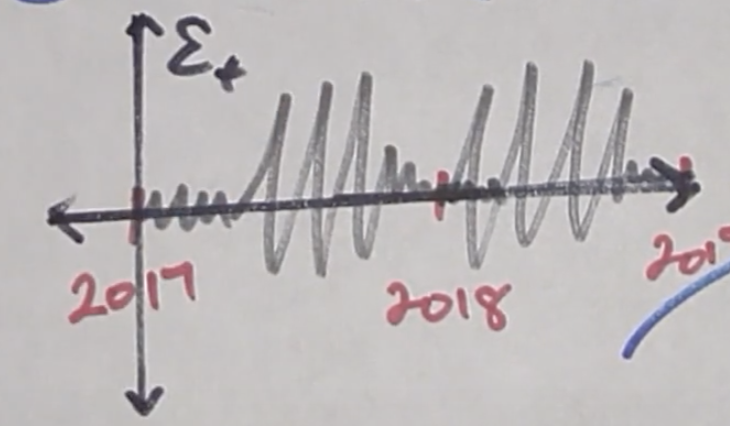
\includegraphics[scale=0.4]{src/ritvikmath-movie-plot-residuals.png}
		\end{enumerate}
	\item	We see that in the middle of each year (summer) way more volatile than the rest of the year but why?
	\item[]	Maybe there's lots of really good and really bad movies in summer so hard to predict;
	\item[]	Beginning of year / end of year, maybe there's better or less movies so more consistent;
	\item	BUT, the important is that there are \textbf{annual patterns} which we could \textbf{use to predict} the sales;
	\item	Enter the \textbf{Auto Regressive Conditional Heteroscedasticity}, or \textbf{Auto Regressive Changing Heteroscedasticity}, (ARCH) Model;
		\begin{itemize}
		\item	Heteroscedasticity just means the \textbf{volatility} is \textbf{not constant};
		\item[]	Logically, we see there's alot of volatility at times but not all the time;
		\item	That's to say, the volatility is \textbf{conditional} on where we are rather than being constant;
		\item	Further more, depending on where we are means we need an \textbf{auto-regressive} model;
		\end{itemize}
	\item	For an ARCH(1) model:
	\item	The variance, or volatility, of the error today $\text{Var}(\varepsilon_{t}) = \sigma^{2}_{t}$ is $\sigma^{2}_{t} = \alpha_{0} + \alpha_{1} \sigma^{2}_{t - 1}$;
	\item[]	That is, a constant $\alpha_{0}$ plus another constant $\alpha_{1}$ time the volatility of yesterday $\varepsilon_{t - 1}$;
	\item[]	So, how crazy, or far, you're swinging from the mean $\alpha_{0}$ today $\sigma^{2}_{t}$ will be a function of how far you were swinging from the mean yesterday $\sigma^{2}_{t - 1}$;
	\item	We then find the formula for the error $\varepsilon_{t}$ as:
	\begin{align*}
		\varepsilon_{t}	&=	w_{t} \sqrt{\alpha_{0} + \alpha_{1} \varepsilon_{t - 1}^{2}}
	\end{align*}
	\item[]	So we have the unpredictible white noise $w_{t}$ times the root of the mean $\alpha_{0}$ plus the square of yesterday's error $\varepsilon_{t - 1}$ multiplied by the trend $\alpha_{1}$;
	\item	Since a square root is only positive, the white noise $w_{t}$ serves as a indicator of whether it'll be negative or positive;
	\item[]	That's why we can go from a very large to a very small value from one period to the next;
	\item	For an ARCH(\textcolor{lava}{2}) this becomes:
	\begin{align*}
		\varepsilon_{t}	&=	w_{t} \sqrt{\alpha_{0} + \alpha_{1} \varepsilon_{t - 1}^{2} \textcolor{lava}{+ \alpha_{2}  \varepsilon_{t - 2}^{2}}}
	\end{align*}
	So today's error is a function of both yesterday and two days ago's error;
	\item	If yesterday's error is large then so will today;
	\item	To better see the \textcolor{blue_rectangle}{auto-regressive} part, we expand the square of the error of a ARCH(1) model:
	\begin{align*}
		\textcolor{blue_rectangle}{ \varepsilon_{t}^{2}}	&=	w_{t}^{2} \alpha_{0} + w_{t}^{2} \alpha_{1} \textcolor{blue_rectangle}{ \varepsilon_{t - 1}^{2}}
	\end{align*}
	\item	For an ARCH(1) model we'd expect to see high auto-correlation between the present error  $\varepsilon_{t}$ and the error lagged by one $\varepsilon_{t - 1}$
	
	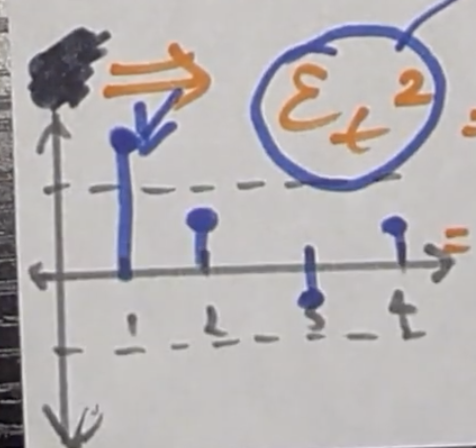
\includegraphics[scale=0.4]{src/ritvikmath-movie-plot-residuals-ARCH.png}
\end{itemize}
\end{YTB_SUMM}

%\begin{YTB_SUMM}{\href{}{ritvikmath: Time Series Talk : }}
%\begin{itemize}
%	\item	
%\end{itemize}
%\end{YTB_SUMM}

\newpage
\chapter[Principal Component Analysis]{Principal Component Analysis (2.5\% à 7.5\%)}

\subsubsection{Information}

\begin{distributions}[Objective]
Understand key concepts concerning Principal Components Analysis
\end{distributions}

\begin{outcomes}[Learning outcomes]
\begin{enumerate}
	\item	Définir des composantes principales
	\item	Interpréter les résultats d'une analyse en composantes principales tout en considérant:
	\begin{itemize}
		\item	\og Loading Factors \fg{} 
		\item	Proportion de la variance expliquée
	\end{itemize}
	\item	Expliquer les utilités et applications de l'analyse en composantes principales
\end{enumerate}
\end{outcomes}

\begin{ASM_chapter}[Related lessons ASM]
\begin{enumerate}
  \setcounter{enumi}{16}
	\item	\hyperref[PCA-KNN]{Principal Component Analysis}
\end{enumerate}
\end{ASM_chapter}

\begin{YTB_vids}[Vidéos YouTube et liens]
\begin{itemize}
	\item	\href{https://blog.bioturing.com/2018/06/14/principal-component-analysis-explained-simply/}{biotutoring: Principal component analysis explained simply (blog)}
	\item	\href{https://blog.bioturing.com/2018/06/18/how-to-read-pca-biplots-and-scree-plots/}{biotutoring: How to read PCA biplots and scree plots (blog)}
	\item	\href{https://www.youtube.com/watch?v=HMOI_lkzW08&list=PLblh5JKOoLUICTaGLRoHQDuF_7q2GfuJF&index=23}{StatQuest: PCA main ideas in only 5 minutes!!!}
%	\item	\href{https://www.youtube.com/watch?v=_UVHneBUBW0&t=16s}{StatQuest: Principal Component Analysis (PCA) clearly explained (2015)} (outdated, focuses on eigenvector approach)
	\item	\href{https://www.youtube.com/watch?v=FgakZw6K1QQ}{StatQuest: Principal Component Analysis (PCA) (step by step)}
	\item	\href{https://www.youtube.com/watch?v=oRvgq966yZg&list=PLblh5JKOoLUICTaGLRoHQDuF_7q2GfuJF&index=24}{StatQuest: PCA - Practical Tips}
%	\item	\href{https://www.youtube.com/watch?v=0Jp4gsfOLMs}{StatQuest: PCA in R} (to watch!)
%	\item	\href{https://www.youtube.com/watch?v=GEn-_dAyYME}{StatQuest: MDS and PCoA}
	\item	\hyperref[MDS-PCOA]{StatQuest: MDS and PCoA}
\end{itemize}
\end{YTB_vids}

\begin{CHPT_SUMM}[label = {PCA-PCA}]{\addcontentsline{toc}{subsubsection}{17. Principal Component Analysis}17. Principal Component Analysis}

Les chapitres 17 et 18 (Cluster analysis) sont des chapitres traitant sur l'apprentissage non supervisé. En apprentissage non supervisé on ne cherche pas à prédire, mais plutôt à apprendre des données. Par exemple, Google qui te suggère des sites selon ce que tu click dessus habituellement, ce que le monde semblable à toi click, etc.

\begin{enumerate}
	\item	\textbf{Loadings} et \textbf{scores}
	\item[]	\textbf{Préliminaire}
		\begin{itemize}
		\item	There is a set of $p$ features (aka independant variables) $X_{1}, \dots, X_{p}$;
		\item	There are $n$ observations;
		\item	Pour toutes les $n$ observations, on soustrait leur moyenne $\bar{x}_{i}$ des $p$ variables $x_{ij}$ pour que la moyenne de chacune des $p$ variables soit nulle:
			\begin{align*}
			\sum_{i = 1}^{n} x_{ij} &= 0, \, \forall \ j = 1, \dots, p
			\end{align*}
		\end{itemize}
	\item[]	\textbf{Description}
		\begin{itemize}
		\item	PCA finds a low-demensional representation of the data set that contains as much as possible of the variation;
		\item	PCA seeks a small number of dimensions that are as \textit{interesting} as possible;
		\item	\textit{interesting} is measured by the amount of variability of the observations along each \textit{dimension} or, \textit{principal component};
		\end{itemize}
	\item[]	\textbf{Finding} the principal components
		\begin{itemize}
		\item	The \textit{first principal component} is the \textit{normalized} linear combination of it's \textit{loadings} $\phi_{11}, \dots, \phi_{p1}$ and the features $X_{1}, \dots, X_{p}$:
			\begin{equation*}
			Z_{1}	=	\phi_{11} X_{1} + \dots + \phi_{p1} X_{p}
 			\end{equation*}
		at the point where it's variance, $\text{Var}(Z_{1})$, is \textit{maximised};
		\item	\textit{maximising} the variance represents explaining as much of the variability of the points as possible;
		\item	\textit{Normalized} means that the $\sum_{j = 1}^{p} \phi_{j1}^{2} = 1$;
		\item[]	Alors, on maximise \textit{sous contraintes}, comme avec Ridge et Lasso, sauf que l'on applique également une \textit{pondération} des variables:
			\setlength{\mathindent}{-1cm}
			\begin{align*}
			\max 
				\left\{ \frac{1}{n} \sum_{i = 1}^{n} \left( \sum_{j = 1}^{p} \phi_{j1} x_{ij} \right)^{2} \right\} \, 
			\text{sous contraite que } 
				\sum_{j = 1}^{p} \phi_{ji}^{2} = 1
			\end{align*}
			\setlength{\mathindent}{1cm}
		\item	Les loadings sont donc des \textit{poids} pour chacune des variables explicatives $X_{1}, \dots, X_{p}$;
		\item	En bref, chaque composante principale, $Z_{i}$, a $p$ loadings, $\phi_{ji}$, sélectionnés en maximisant sa variabilité;
		\item	De plus, pour maximiser les composantes principales après 1 on ajoute la contrainte que $Z_{m}$ n'est pas corrélé avec $Z_{k}$ pour tout $k < m$;
		\item[]	Ceci est fondé sur l'algèbre linéaire et les \textit{eigenvectors} mais ce n'est pas dans le cadre de l'examen;
		\item[]	Cela dit, l'idée est que pour ne pas être corrélé la deuxième composante principale direction sera \textbf{orthogonale} à la première;
		\item[]	Pour la suite, chaque composante principale sera orthogonale à l'hyperplan des composantes principales précédentes;
		\end{itemize}
	\item[]	\textbf{Scores} des observations
		\begin{itemize}
		\item	Chacune des $n$ observations ont des \og coordonnées \fg{} $z_{ki}$ dans le \textit{$Z$ coordinate system} surnommées des \textbf{scores};
		\item	Il y a $p$ scores pour chacune des $n$ observations;
		\item[] Pour example, les scores de la première observation sont:
			\begin{align*}
			z_{k1}	&=	\sum_{j = 1}^{p} \phi_{j1} x_{kj}, \ k = 1, \dots, n
			\end{align*}
		\item	Donc, chaque composante principale trouvé avec est une \textit{combinaison linéaire} des $p$ features;
		\item	Alors on \textit{réduit les \textbf{dimensions}}, le nombre de variables, avec des \textit{\textbf{combinaisons} des variables} existantes corrélées;
		\item[]	En contraste, Ridge \textit{réduit les \textbf{coefficients}} des variables corrélées;
%		\item	Le score $i$ de l'observation $k$ est la distance du point $k$ de 0, dans la direction, ou \textit{dimension}, $Z_{i}$;
		\item	Le plus faible le \textit{score}, le plus corrélé ou près les points;
		\item 	Cependant, il peut s'avérer compliqué d'interpréter juste des chiffres et donc nous avons le \textit{biplot};
		\end{itemize}
%%%		
	\item	\textbf{Biplots}
	\begin{itemize}
		\item	Un biplot plot à la fois les loading vector (voir vidéo de StatQuest, très bien expliqué) et les loading scores;
		\item[]	Les loadings vectors aident à visualiser dans quelle direction chacune des variables est dirigée;
		\item[]	Les loadings scores sont les coordonnées des observations;
		
		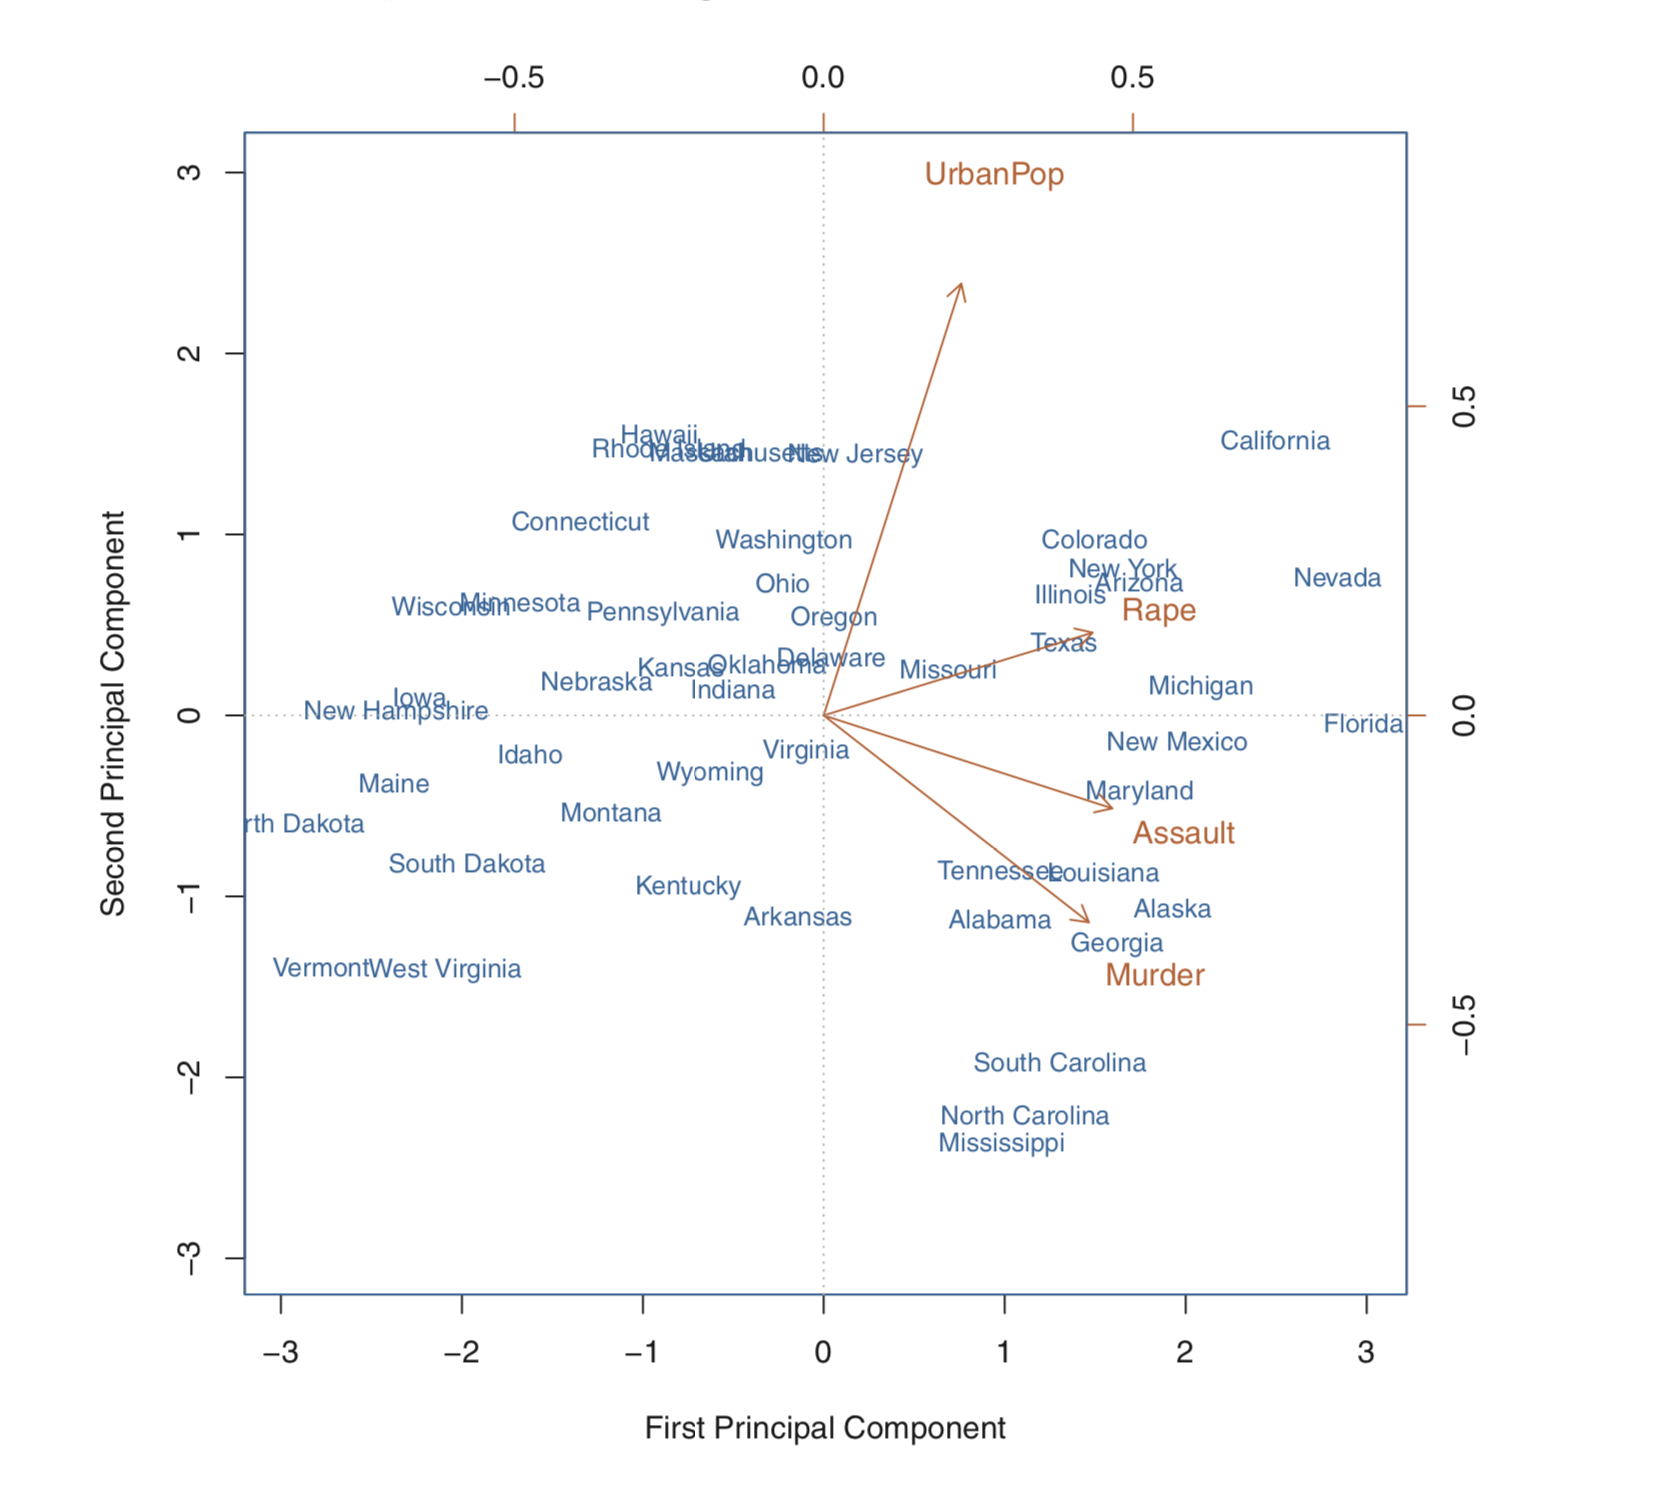
\includegraphics[scale=0.4]{src/PCA-BIPLOT.png}
		\item	On peut donc, entres autres, en déduire:
			\begin{itemize}
			\item	l'influence de chaque variable sur les observations;
			\item	Si des vecteurs de direction sont semblables alors les variables se recoupent;
			\item	Si des points sont plus dans un coin que l'autre, selon les vecteurs, on peut déduire quelles variables ont un plus gros impact;
			\item	On peut d'ici faire des regroupements de points semblables, etc.;
			\end{itemize}
		\item	On note que les variables du graphique ci-dessus sont standardisées;
		\item[]	Donc, la majorité des points sont entre -3 et 3 (99.7\% des points d'une distribution normale standardisée sont entre -3 et 3);
		
	\end{itemize}
%%%	
	\item	Approximation and scaling
	\item[]	\textbf{Approximation}
	\begin{itemize}
		\item	Nous développons davantage la discussion sur les composantes principales comme	 des surfaces linéaires à basse dimension les \textit{plus près} des observations;
		\item	Par exemple, pour la première composante principale: 
		
		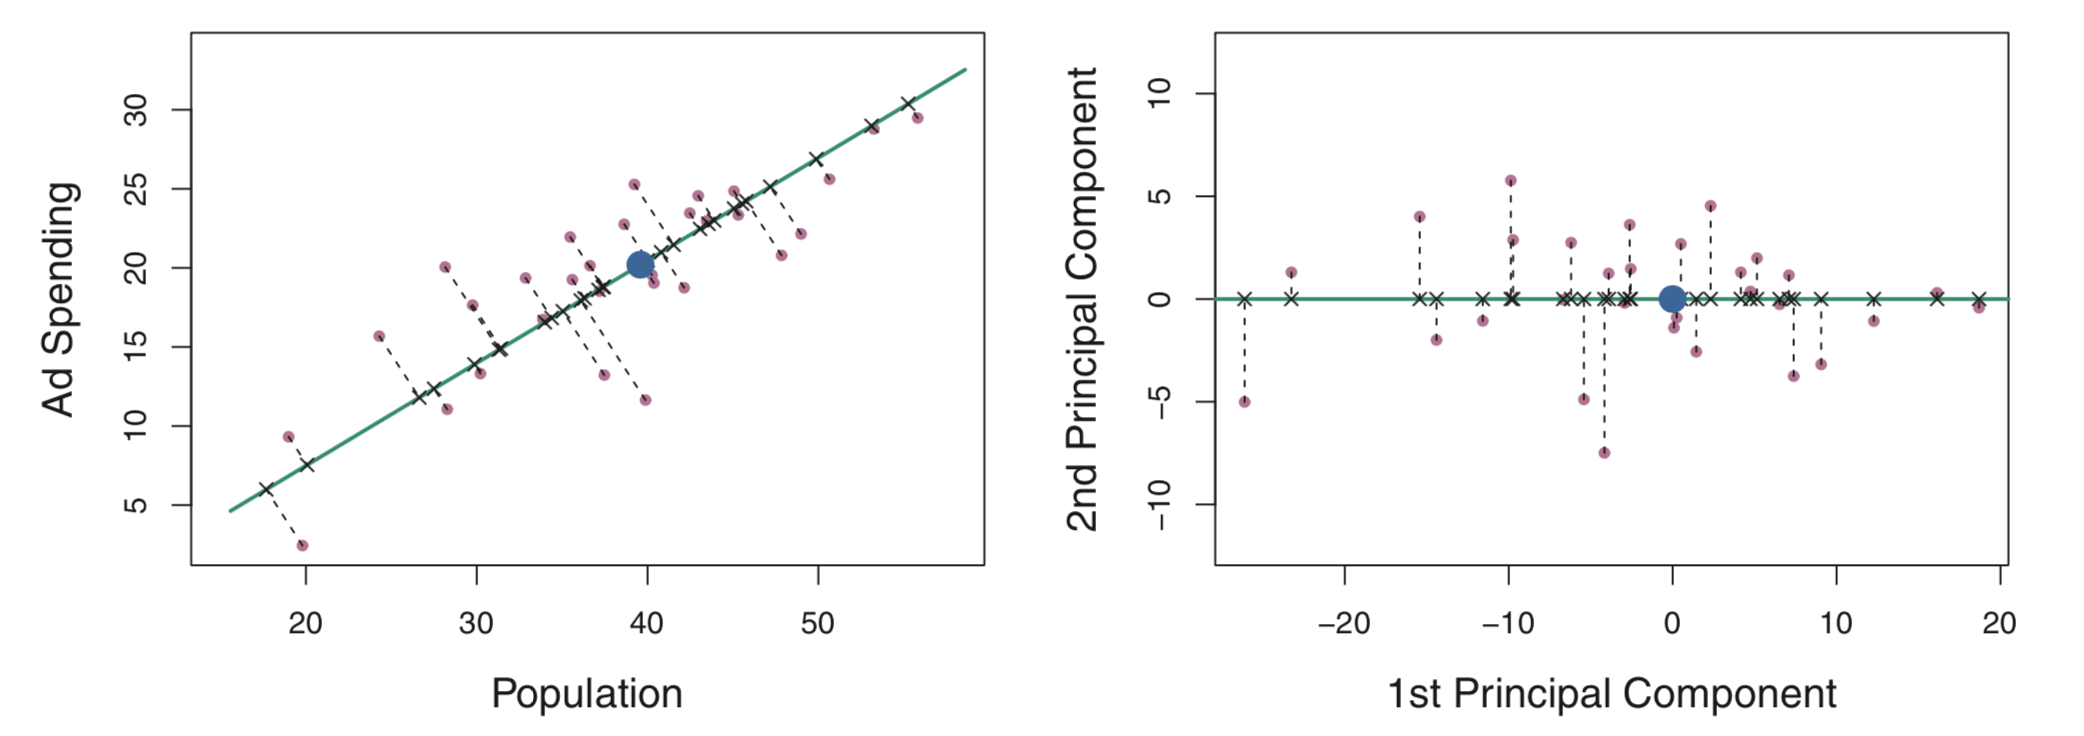
\includegraphics[scale=0.3]{src/PCA-2D-CLOSEST.png}
		\item	Donc, les erreurs (pointillés à gauche) sont minimisées;
		\item	Cette idée est la même dans les prochaines dimensions, pour exemple la 3ème :
		
		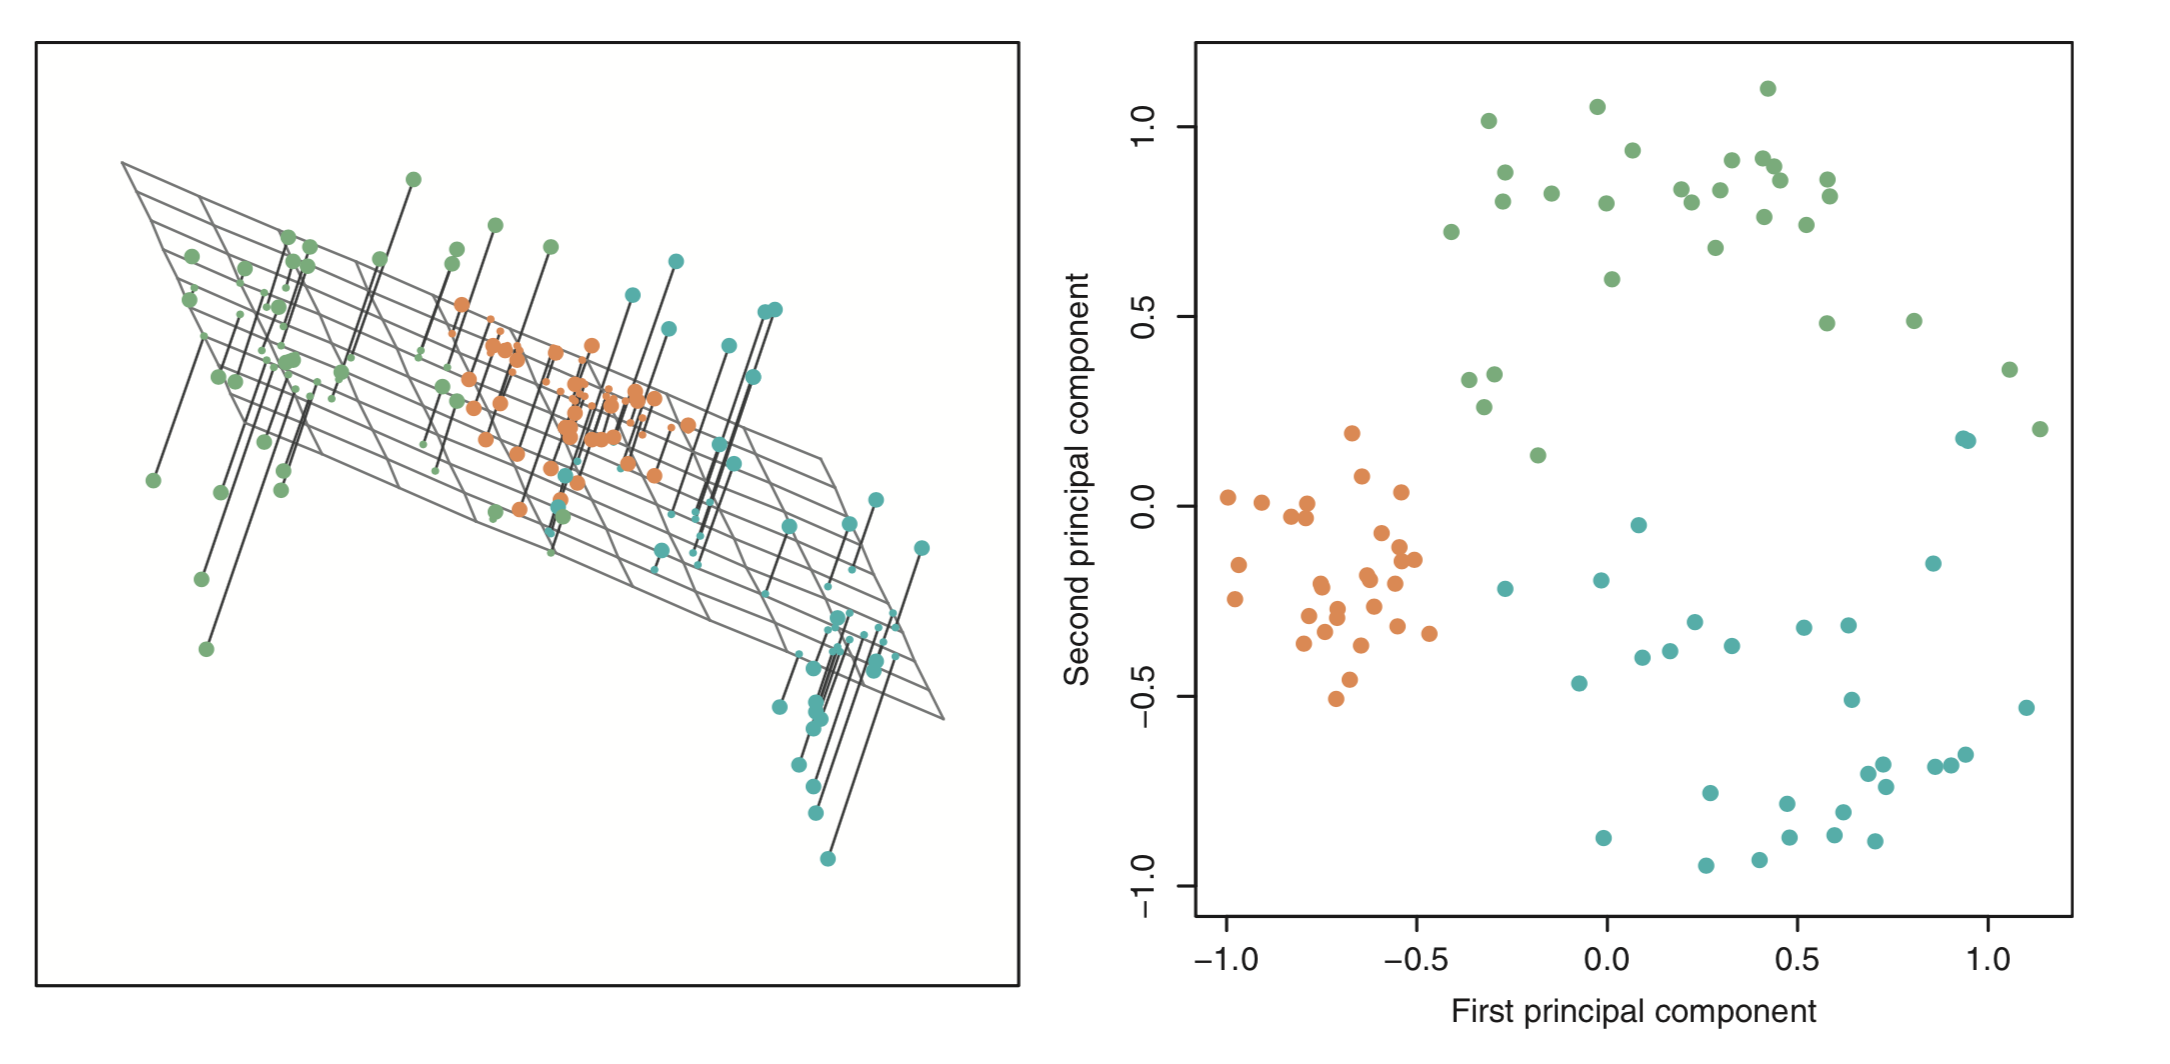
\includegraphics[scale=0.28]{src/PCA-3D-CLOSEST.png}
		\item	Ce faisant, les $k$ premières composantes principales sont la meilleure approximation à $k$ dimensions de la $i$ème observation $x_{ij}$;
		\item	Lorsque les variables sont centrées à 0, l'approximation de la $j$ème composante de la $i$ème observation est:
			\begin{align*}
			x_{ij}	&\approx	\sum_{m = 1}^{M} z_{im} \phi_{jm}
			\end{align*}
		\item	Cette approximation est donc logiquement exacte si tous les PC sont utilisés, $M = \min(n - 1, p)$, et est une bonne approximation puisque d'habitude avec 2 PCs on expliquer la majorité de la variabilité;
	\end{itemize}
	\item[]	\textbf{Unique}: On rappel que des \textit{eigenvalues sont uniques}. 
			Ce faisant, peut importe le programme utilisé, le vecteur de composantes principales sera toujours le même;
	\item[]	\textbf{Scaling}
		\begin{itemize}
		\item	L'échelle a une grande importance pour l'analyse en composantes principales;
		\item	En régression linéaire, si une variable $x$ est multipliée par $r$ on peut diviser $\beta$ par $r$;
		\item[]	Puisque nous avons des combinaisons linéaires en PCA, ceci n'est pas vrai et pourrait biaiser les résultats;
		\item	Habituellement, on \textit{pondère par l'écart-type};
		\item	Voici un exemple du live qui rend évident la distinction:
		
		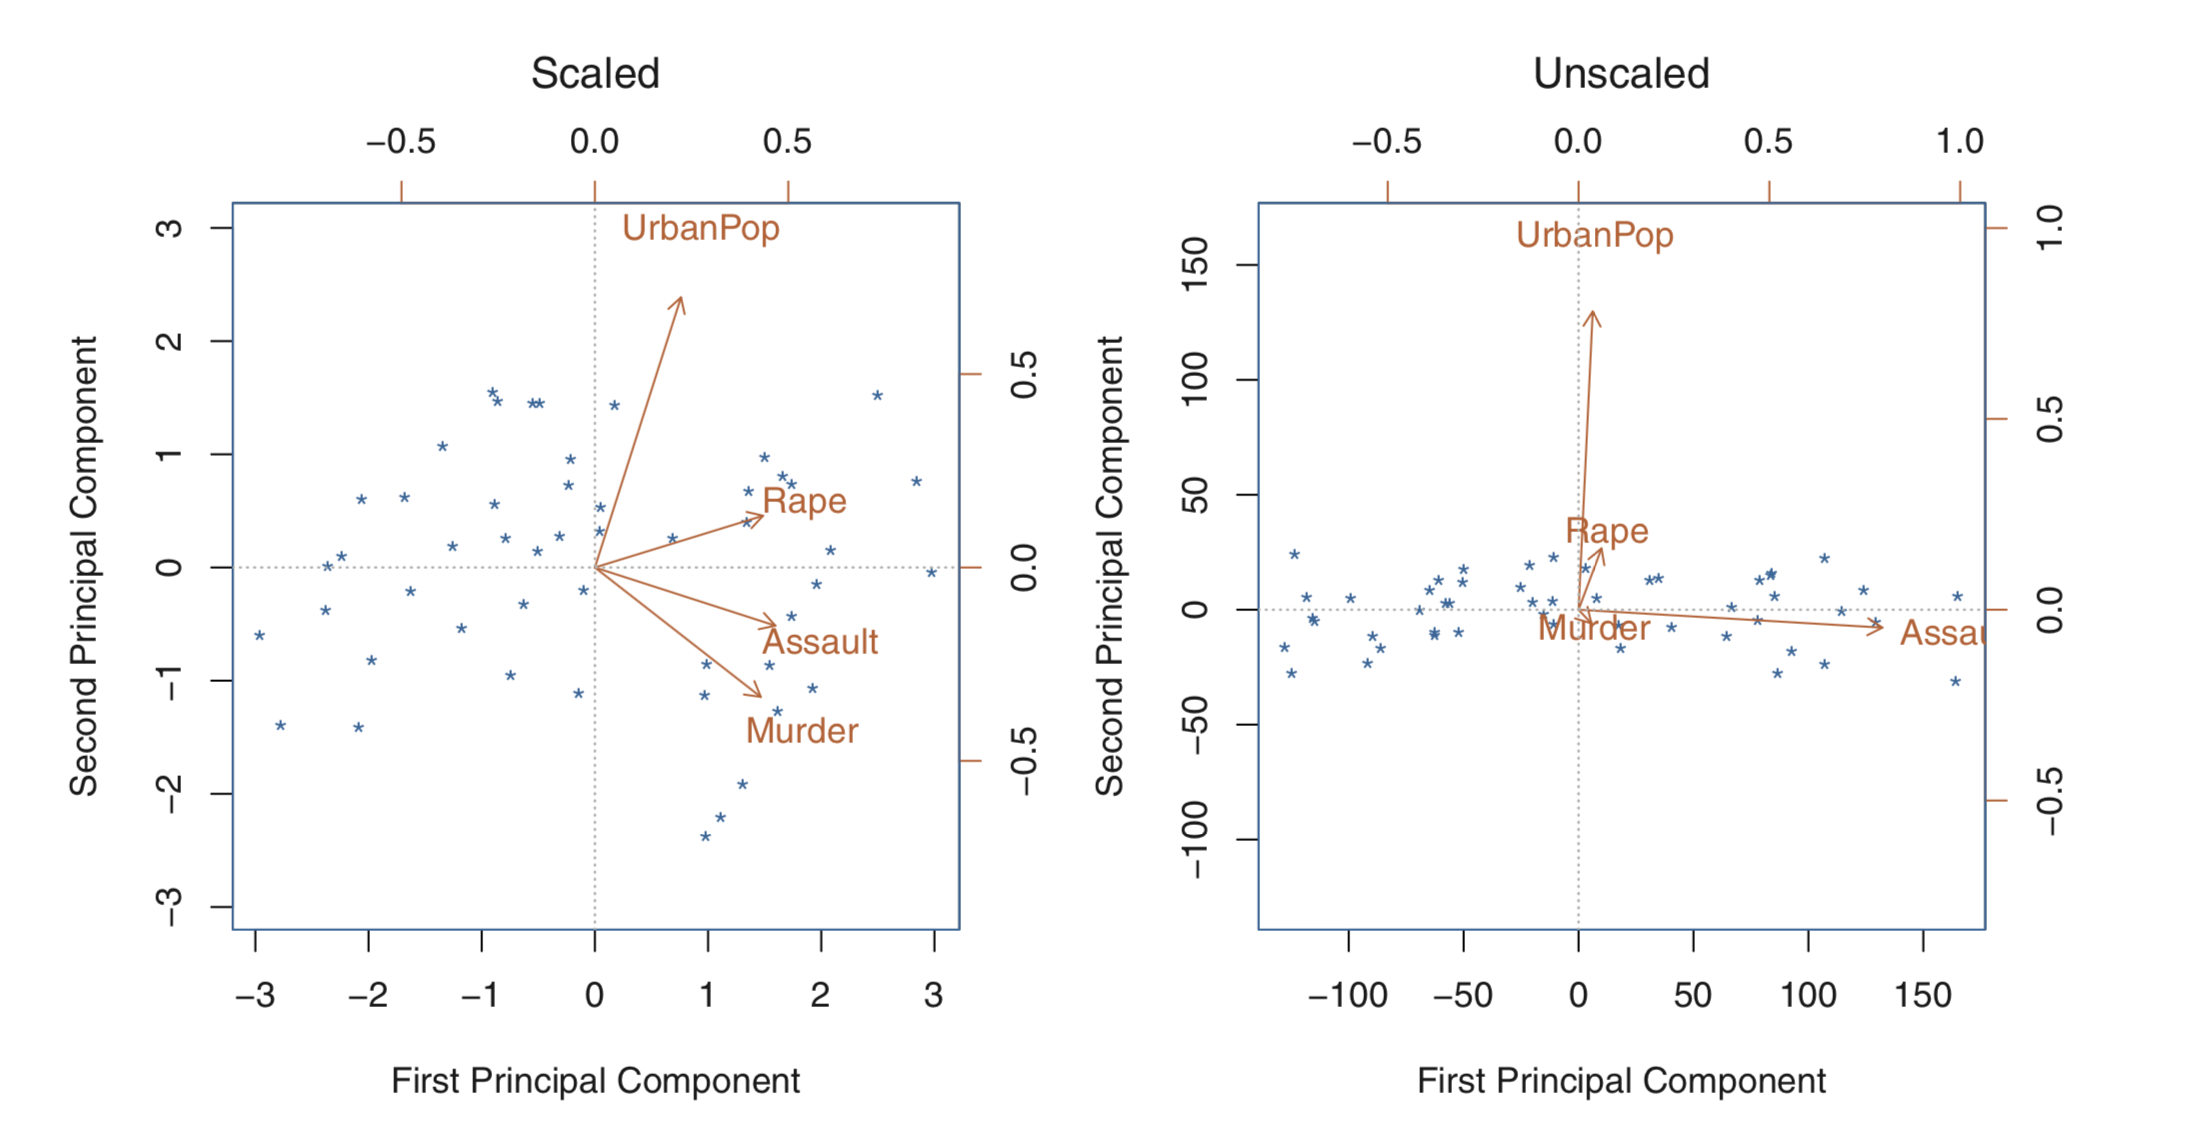
\includegraphics[scale=0.25]{src/PCA-SCALING.png}
		\end{itemize}
%%%	
	\item	\textbf{Proportion of variance explained} (PVE)
		\begin{itemize}
		\item	Puisqu'on sait qu'en réduisant on ne capture pas toute la variabilité, on veut savoir combien qu'on en perds?
		\item	Donc, on veut la \textbf{Proportion de Variance Expliquée \textit{(PVE)}} pour chacune des composantes principales;
		\item	La \textit{variance totale} d'un ensemble de données, en prenant pour acquis que les variables sont centrées à 0, est:
			\begin{align*}
			\sum_{j = 1}^{p} \text{Var}(X_{j})	&=	\sum_{j = 1}^{p} \frac{1}{n} \sum_{i = 1}^{n} x_{ij}^{2}
			\end{align*}
		\item	La \textit{variance expliquée} par la $m$ème composante principale est:
			\begin{align*}
			\text{Var}(Z_{m})
			&=	\frac{1}{n} \sum_{i = 1}^{n}	z^{2}_{im} \\
			&= \frac{1}{n} \sum_{i = 1}^{n} \left( \sum_{j = 1}^{p} \phi_{jm} x_{ij} \right)^{2}
			\end{align*}
		\item	La \textit{\textbf{proportion} de la variance expliquée} par la $m$ème composante principale est donc:
			\begin{align*}
			PVE	
			&=	\frac{\text{Var}(Z_{m})}{\sum_{j = 1}^{p} \text{Var}(X_{j})}	\\
			&=	\frac{\sum_{i = 1}^{n} \left( \sum_{j = 1}^{p} \phi_{jm} x_{ij} \right)^{2}}{\sum_{j = 1}^{p} \sum_{i = 1}^{n} x_{ij}^{2}}	
			\end{align*}
		\item	On peut calculer la PVE cumulative pour M composantes principales jusqu'à un certain seuil pour sélectionner un M;
		\item	On peut aussi regarder un screen plot jusqu'à ce qu'on ai un \textit{elbow} satisfaisant;
		\end{itemize}
\end{enumerate}

\textbf{Note sur les exercices:} 
\begin{enumerate}
	\item	Calculer des scores ou loadings de données partielles (1 à 3);
	\item	Questions qualitatives sur le PCA (4, 5);
	\item	Questions dont il faut \textbf{interpréter le graphique} comme 7;
	\item	Calculer un PVE comme 6;
	\item	Si question à, pour exemple, $p = 2$ et $\phi_{11} = 0.73$ et stipule $k < 0$ alors $\phi_{12} = -\sqrt{1 - 0.73^{2}}$. Alias, un ajoute un négatif;
\end{enumerate}
\end{CHPT_SUMM}

\subsection{Notes sur les vidéos YouTube}

\begin{YTB_SUMM}{\href{https://www.youtube.com/watch?v=FgakZw6K1QQ}{StatQuest : Principal Component Analysis (PCA) (step by step)}}
\begin{itemize}
	\item	We plot the data and find the middle of it;
	\item	Afterwards, we shift the data to center it at the origin ($0$, $0$);
	\item	From here, we want to fit a line to the data;
	\item[]	We note that the distance from the point to the origin, $a$, is constant;
	\item[]	However, both the distance from the point to the line, $b$, and from the projection of the point on the line to the origin, $c$, are variable;
	\item	Usually, we minimise the distance of the points to the line (the error);
	\item[]	However, in PCA it's actually easier to \textit{maximise} the distance of the \textit{projection to the origin} and that is \textbf{equivalent} as per the \textit{Pythagorean theorem};
	\item	To fully understand this, it's imperative to see how this image moves around in the video or \href{https://cdn-images-1.medium.com/max/800/0*XqrkXQoEQEIRe0Nm}{this gif}	:	
	
	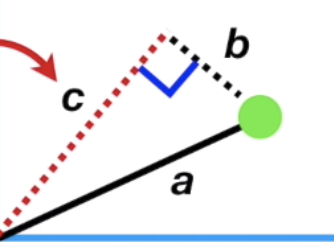
\includegraphics[scale=0.4]{src/SQ-PCA-PYTHAGOREAN.png}
	\item	The ratio 4 to 1 means the data is mostly spread out along the gene 1 axis---4 times more spread out in fact;
	\item[]	We can think of it as a cocktail mixture:
		\begin{enumerate}
		\item	Mix \textbf{4} parts gene 1;
		\item	Mix \textbf{1} part gene 2;
		\item	Pour over ice and serve;
		\end{enumerate}
	\item[]	This is called a \textit{linear combination} of genes 1 and 2;
	\item	Thus, we got the following unit vector:
	
	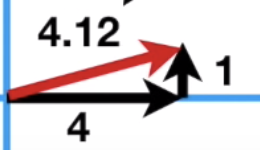
\includegraphics[scale=0.4]{src/SQ-PCA-unit-vector.png}
	\item	To get a 1 unit long vector, we scale both sides by 4.12 (length of $c$);
	\item	Thus, we get a new recipe for which the \textit{proportions are the same} but the parts changed: 
		\begin{enumerate}
		\item	Mix \textbf{0.97} part gene 1;
		\item	Mix \textbf{0.242} part gene 2;
		\item	Pour over ice and serve;
		\end{enumerate}
	\item[]	This vector is called the \textit{singular vector} or \textbf{eigenvector};
	\item[]	The proportions of each gene are the \textbf{loading scores};
	\item	Finally, the sum of squared distances from the projection to the origin is the Sum of Squared distances SS(distances):
	
	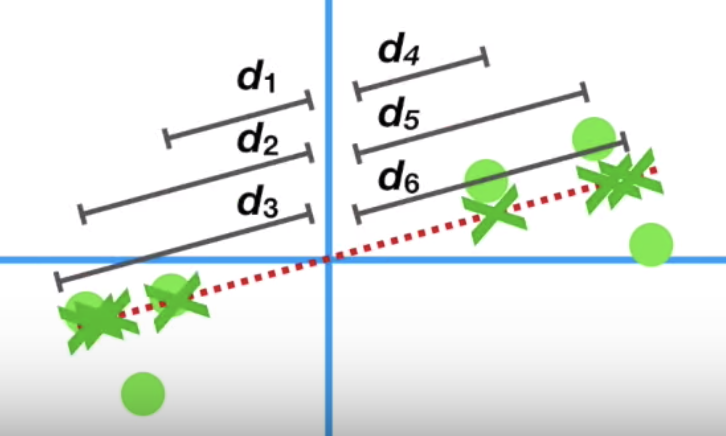
\includegraphics[scale=0.4]{src/SQ-PCA-SSD.png}
	\item	The SS(distances) for the \textit{best fit line} is then called the \textbf{eigenvalue} for the first principal component PC1;
	\item[]	It's square root, $\sqrt{\text{Eigenvalue for PC1}}$, is the \textit{singular value};
	\item	PC2 then becomes the line through the origin \textit{perpendicular} to PC1;
	\item	It's cocktail recipe and scaling is the same procedure as before:
		\begin{enumerate}
		\item	Mix \textbf{-1} part gene 1 -> -0.242 part gene 1;
		\item	Mix \textbf{4} parts gene 2 -> 0.97 part gene 2;
		\item	Pour over ice and serve;
		\end{enumerate}
	\item	The unit vector in blue is thus the \textit{singular vector}, or \textit{eigenvector}, for PC2;
	
	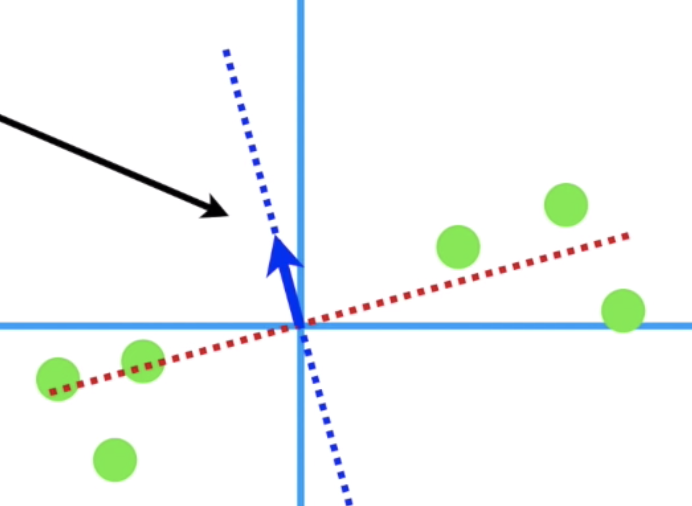
\includegraphics[scale=0.4]{src/SQ-PCA-unit-vector-PC2.png}
	\item	The interpretation, in terms of how the values are \textit{projected} onto PC2:
	
	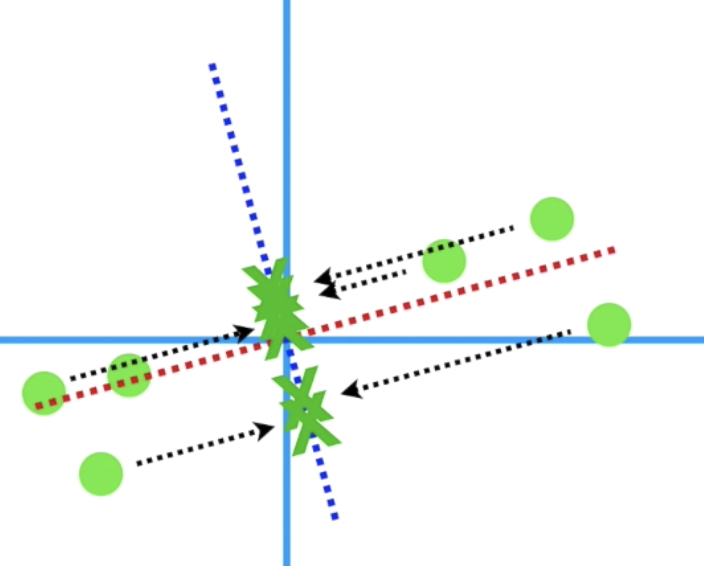
\includegraphics[scale=0.4]{src/SQ-PCA-unit-vector-PC2-projection.png}
	
	is that gene 2 is 4 times more important than gene 1;
	\item	Finally, like for PC1, the \textit{eigenvalue} is the SS(distances) between projected points and the origin:
	
	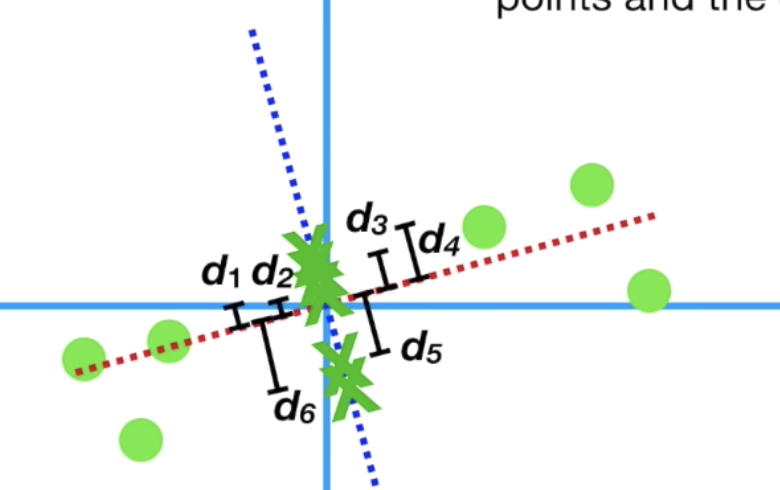
\includegraphics[scale=0.4]{src/SQ-PCA-SSD-PC2.png}
	\item	The PCA plot is thus the rotation of the graph with the principal components as the axes;
	\item[]	The samples are mapped with the loadings as the ($x$, $y$) coordinates;
	
	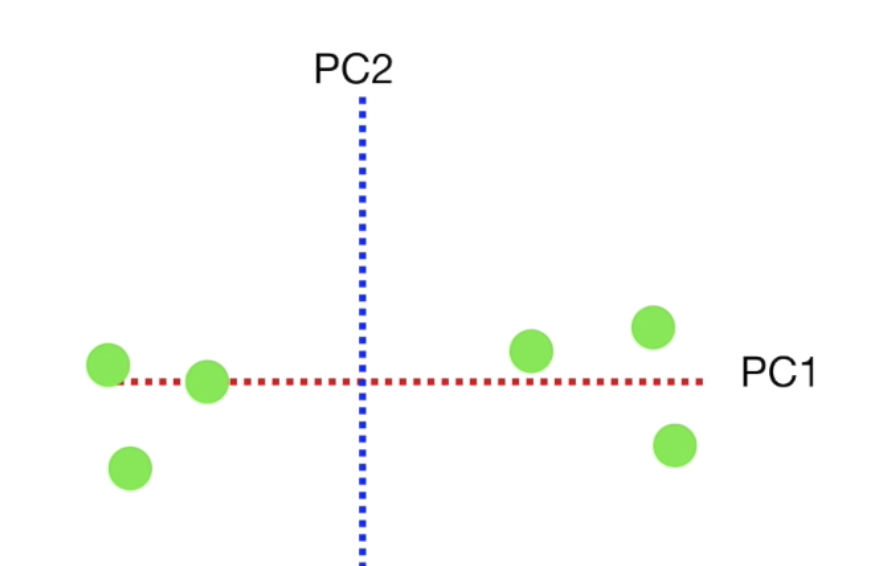
\includegraphics[scale=0.4]{src/SQ-PCA-PCA-plot.png}
	
	\item	For variation, imagine the variation of PC1 is 15 and of PC2 is 3;
	\item[]	Thus, PC1 accounts for 83\% of the variation and PC2 17\%;
	\item	We can make a plot of these percentages and that's called a \textit{scree} plot:
	
	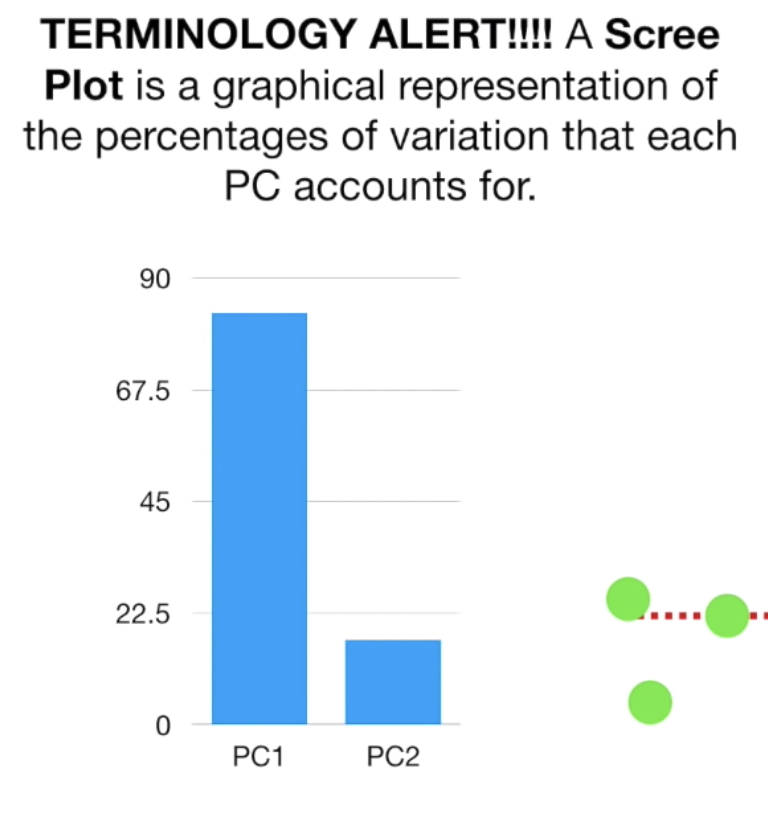
\includegraphics[scale=0.4]{src/SQ-PCA-scree-plot.png}
	\item	Example with 3 PC
	\item	The number of PCs is usually the minimum between the number of variables and observations;
	\item	Once we have all the PCs, we can use the SS(distances), a.k.a. \textit{eigenvalues}, to determine the proportion of variance each PC accounts for;
	\item	We see from the scree plot that PC1 and PC2 already explain 94\% of the variation and that just those 2 vectors would be a good approximation;
\end{itemize}
\end{YTB_SUMM}

\begin{YTB_SUMM}{\href{https://www.youtube.com/watch?v=oRvgq966yZg&list=PLblh5JKOoLUICTaGLRoHQDuF_7q2GfuJF&index=24}{StatQuest: PCA - Practical Tips}}
\begin{enumerate}
	\item	\textbf{Scaling} your data: Make sure variables are on the same scale and, if not, scale them.
		\begin{itemize}
		\item	For example, math scores between 0 and 100 vs English scores between 0 and 10;
		\item	We'd then have 99 parts math to 1 part reading;
		\item	But that's only because the math scale is 10 times that of reading scores;
		\item	In reality, it's a 1 to 1 relationship!;
		\item	Thus, ensure scales are \textit{roughly} equivalent otherwise will be biased towards one of them;
		\item	This is usually done with the standard deviation;
		\end{itemize}
	\item	Centering your data: Make sure your data is centered.
		\begin{itemize}
		\item	Not always done by default;
		\item	If I try SVD without centering, it will still try to fit a line through the origin which can become ridiculous;
		\end{itemize}
	\item	How many PC can you expect to find?
		\begin{itemize}
		\item	in 2D there's no way to draw a perpendicular line to both PC1 and PC2;
		\item	So, if we've only measured 2 things then we couldn't have more than 2 PCs;
		\item	With 2 points we can only have a line;
		\item	A plan requires at least 3;
		
		\end{itemize}
\end{enumerate}
\end{YTB_SUMM}

\begin{YTB_SUMM}[label = MDS-PCOA]{\href{https://www.youtube.com/watch?v=GEn-_dAyYME}{StatQuest: MDS and PCoA}}
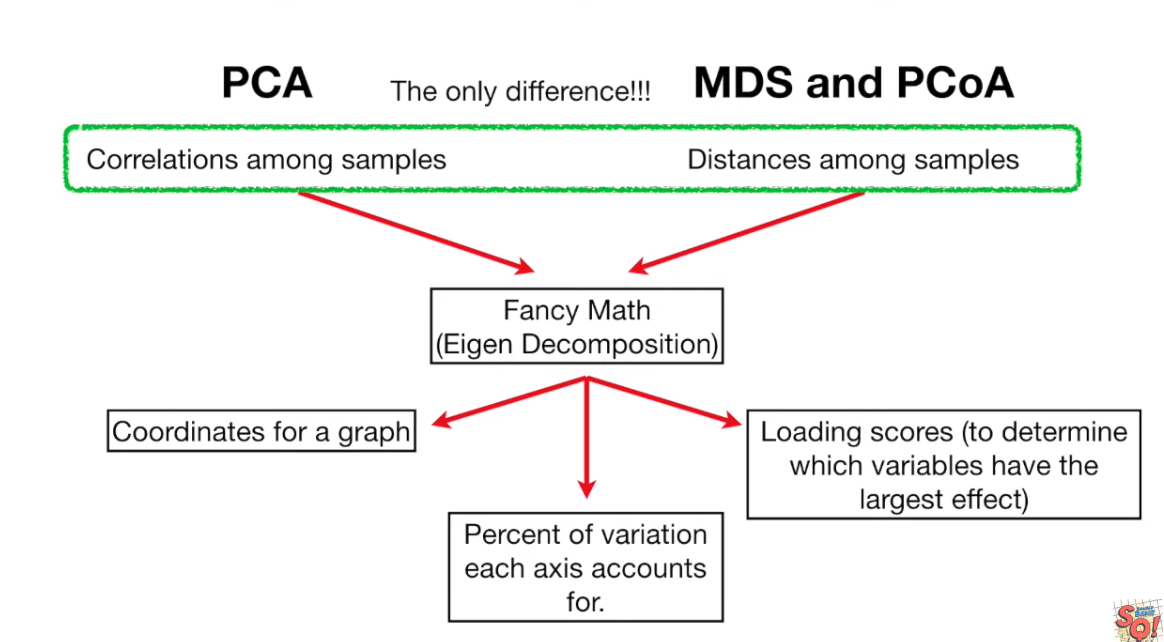
\includegraphics[scale=0.3]{src/SQ-PCA-PCOA.png}
\end{YTB_SUMM}

\newpage
\chapter[Decision Trees]{Decision Trees (10\% à 15\%)}

\subsubsection{Information}

\begin{distributions}[Objective]
Understand key concepts concerning decision tree models
\end{distributions}

\begin{outcomes}[Learning outcomes]
\begin{enumerate}
	\item	Expliquer l'utilité et les applications des arbres de décisions.
	\item	Expliquer et interpréter les arbres de décisions en considérant les arbres de régression et le \og recursive binary splitting \fg{}.
	\item	Expliquer et interpréter le \og bagging \fg{}, \og boosting \fg{} et les forêts aléatoires.
	\item	Expliquer et interpréter les arbres de classification, leur construction, le \og Gini Index \fg{} et \og entropy \fg{}.
	\item	Comparer les arbres de décisions aux modèles linéaires.
	\item	Interpréter les résultats d'une \og decision tree analysis \fg{}.
\end{enumerate}
\end{outcomes}

\begin{ASM_chapter}[Related lessons ASM]
\begin{enumerate}
  \setcounter{enumi}{15}
	\item	\hyperref[DECISION-TREES]{Decision Trees}
\end{enumerate}
\end{ASM_chapter}

\begin{YTB_vids}[Vidéos YouTube]
\begin{itemize}
	\item	\href{https://www.youtube.com/watch?v=7VeUPuFGJHk&list=PLblh5JKOoLUICTaGLRoHQDuF_7q2GfuJF&index=34}{StatQuest: Decision Trees}
%	\item	\hyperref[TREES-PART1]{StatQuest: Decision Trees}
	\item	\href{https://www.youtube.com/watch?v=wpNl-JwwplA&list=PLblh5JKOoLUICTaGLRoHQDuF_7q2GfuJF&index=35}{StatQuest: Decision Trees, Part 2 - Feature Selection and Missing Data}
%	\item	\hyperref[RANDOMFORESTS-BAGGING]{StatQuest: Decision Trees, Part 2 - Feature Selection and Missing Data}
%	\item	\href{https://www.youtube.com/watch?v=g9c66TUylZ4&list=PLblh5JKOoLUICTaGLRoHQDuF_7q2GfuJF&index=36}{StatQuest: Regression Trees, Clearly Explained!!!}
	\item	\hyperref[TREES-REGRESSION]{StatQuest: Regression Trees, Clearly Explained!!!}
%	\item	\href{https://www.youtube.com/watch?v=D0efHEJsfHo&list=PLblh5JKOoLUICTaGLRoHQDuF_7q2GfuJF&index=37}{StatQuest: How to Prune Regression Trees, Clearly Explained!!!}
	\item	\hyperref[TREES-PRUNING]{StatQuest: How to Prune Regression Trees, Clearly Explained!!!}
	\item	\href{https://www.youtube.com/watch?v=J4Wdy0Wc_xQ}{StatQuest: Random Forests Part 1 - Building, Using and Evaluating} (Bagging too)
	\item	\href{https://www.youtube.com/watch?v=sQ870aTKqiM}{StatQuest: Random Forests Part 2: Missing data and clustering}
	\item	\href{https://www.youtube.com/watch?v=6EXPYzbfLCE}{StatQuest: Random Forests in R}
	\item	\href{https://www.youtube.com/watch?v=LsK-xG1cLYA}{StatQuest: AdaBoost, Clearly Explained}
\end{itemize}
\end{YTB_vids}

\subsection{Résumés des chapitres}

\begin{CHPT_SUMM}[label = {DECISION-TREES}]{\addcontentsline{toc}{subsubsection}{16. Decision Trees}16. Decision Trees}
Les arbres de décisions sont un alternatif à la régression comme le KNN (chapitre 15). 

\begin{enumerate}
	\item	Building decision trees
%	
	\item[]	Ressemblance au KNN
		\begin{itemize}
		\item	Les arbres de décision sont non paramétriques;
		\item	Ils séparent les prédicteurs en régions;
		\item[]	Les régions sont toujours des carrés multidimensionnels (voir \hyperref[fig:KNN-3D]{l'image 3D du $K$-NN});
		\item	Dans un contexte de \textit{régression}, ils attribuent la \textit{valeur moyenne};
		\item	Dans un contexte de \textit{classification}, ils attribuent la valeur la \textit{plus courante};
		\end{itemize}
%		
	\item[]	\textbf{Liens}
		\begin{itemize}
		\item	Les arbres de décisions sont très utile pour l'interprétation, mais leur puissance de prévision n'est pas aussi bonne que celle des meilleurs approches d'apprentissage (PCA, splines, \dots);
		\item	Ce faisant, les méthodes de \textit{bagging}, \textit{random forests}, and \textit{boosting} produisent plusieurs arbres avant de les combiner et en retirer une prévision;
		\item	L'idée est que combiner beaucoup d'arbres peut significativement augmenter la puissance de prévision au dépens de la facilité d'interprétation;
		\item	Du fait, des algorithmes d'arbres de décisions sont surnommés des \textbf{CART}s \textit{(Classification and Regression Trees)};
		\end{itemize}
%		
	\item[]	\textbf{Composantes} et \textbf{termes}
		\begin{itemize}
		\item	\textbf{Nœuds};
			\begin{itemize}
%			\item	\textit{Root} node: population initiale;
			\item	Nœud \textit{terminal} (feuille): fin de l'arbre;
			\item[]	Chaque feuille correspond à une classe;
			\item	Nœud \textit{interne} (intermédiaire): Nœud se séparant en deux branches;
			\item[]	Chaque nœud interne correspond à un attribut;
			\end{itemize}
		\item	Nœuds dit \textit{Parent} et \textit{Child}: Un nœud séparé en sous-nœuds est le nœud \textit{parent} des sous-nœuds, et les sous-nœuds les nœuds \textit{child};
		\item	\textbf{Splitting} est la division d'un nœud en 2, ou plus, sous-nœuds;
		\item[]	Chaque split est \textit{binaire};
		\item	L'inverse est le \textbf{pruning}, le retrait de sous-nœuds;
		\item	\textbf{Types} de variables
			\begin{itemize}
			\item	Catégoriques:
			\item	Discrètes (count): 
			\item	Continues: 
			\item[]	Un \textit{cut point} doit être choisit dans le cas de variables continues
			\end{itemize}
		\end{itemize}
%		
	\item[]	Arbre optimal (variable continu)
		\begin{itemize}
		\item	Soit $J$ régions $R_{j}$;
		\item	Le MSE est de forme:
			\begin{align*}
			\sum_{j = 1}^{J}	\sum_{i \in R_{j}} (y_{i} - \hat{y}_{i})^{2}
			\end{align*}
				où $\hat{y}_{i}$ est la prévision pour le $i$e point dans la $j$e région;
		\item	\textit{En théorie}, l'arbre optimal est celui qui minimise le MSE;
		\item	\textit{En pratique}, il n'est pas faisable de calculer ceci pour toutes les possibilités;
		\item	Ce faisant, on fait pousser les arbres avec du \textit{recursive binary splitting};
		\end{itemize}
%		
	\item[]	Faire pousser l'arbre
		\begin{itemize}
		\item[]	L'algorithme choisit le binary split qui minimise le MSE;
		\item	L'algorithme est dit \textit{greedy} puisqu'il optimise selon l'étape présente et non le reste de l'arbre;
		\item[]	Comme avec la sélection stepwise, on n'a donc \textit{aucune garantie} d'obtenir la \textit{meilleur optimisation};
		\item	À chaque itération, on choisit: 
			\begin{enumerate}
			\item	Une région à splitter $R_{j}$;
			\item	Un prédicteur $X_{k}$;
			\item	Un cut point $s$;
			\end{enumerate}
		\item[]	tel que le split en $R_{j_{1}}$ et $R_{j_{2}}$ minimise :
			\begin{align*}
			\sum_{i:x_{i} \in R_{j_{1}}} (y_{i} - \hat{y}_{R_{j_{1}}})^{2} + 
			\sum_{x_{i} \in R_{j_{2}}} (y_{i} - \hat{y}_{R_{j_{2}}})^{2}
			\end{align*}
		\item[]	jusqu'à ce que le nombre d'observations dans une région soit inférieur à un certain nombre;
		\end{itemize}
%		
	\item[]	Réduction de l'arbre
		\begin{itemize}
		\item	L'arbre résultant sera assurément trop grand;
		\item	Plus de splits implique davantage de flexibilité, moins de biais et une variance plus élevée;
		\item[]	Ce faisant, il existe un nombre de splits optimal qui minimise le MSE de test;
		\item	Dans la même ordre d'idée que le budget alloué avec l'optimisation Lasso, on \textbf{prune} l'arbre de décision;
		\item[]	Ceci est le \textit{cost complexity}, ou \textit{weakest link}, pruning;
		\item	On spécifie un \textit{tuning parameter} $\alpha$ qui représente le \og coût \fg{} par nœud terminal de l'arbre;
		\item	Pour chacune des valeurs de $\alpha$, on \textit{prune} l'arbre pour minimiser: 
			\begin{align*}
			\sum_{m = 1}^{|T|} \sum_{i:x_{i} \in R_{m}} (y_{i} - \hat{y}_{R_{m}})^{2} + \alpha |T|
			\end{align*}
			où $|T|$ est le nombre de nœuds terminal de l'arbre;
		\item	Nous sélectionnons alors le $\alpha$ optimal selon la \textit{validation croisée};
		\end{itemize}
%		
	\item[]	Arbre optimal (classification)
		\begin{itemize}
		\item	Au lieu du MSE, on cherche à minimiser le \textit{classification error rate}:
			\begin{align*}
			\sum_{j = 1}^{J} \sum_{i \in R_{j}} \Pr(y_{i} \neq \hat{y}_{R_{j}})
			\end{align*}
		\item	Pour une région $R_{j}$ et les classes $1, 2, \dots, K$, $\hat{y}_{R_{j}}$ est la classe la plus fréquente;
		\item	Soit la proportion $p_{jk}$ des observations dans $R_{j}$ pour lesquelles $y_{i} = k$, le \textit{classification error rate} de la région $R_{j}$ est:
			\begin{align*}
			E_{j}	=	1 - \underset{k}{\max} \hat{p}_{jk}
			\end{align*}
		\item	Mais, cette mesure n'est pas assez sensible pour faire pousser les arbres;
		\item	En lieu, on utilise soit le \textit{Gini index} ou l'\textit{entropie croisée};
		\end{itemize}
%		
	\item[]	Mesures de splitting
		\begin{itemize}
		\item	Pour une région $R_{j}$, le Gini index est la variance des observations: 
			\begin{align*}
			G_{j}	&=	\sum_{k = 1}^{K} \hat{p}_{jk} (1 - \hat{p}_{jk})
			\end{align*}
		\item	Pour une région $R_{j}$, l'entropie croisée est:
			\begin{align*}
			D_{j}	&=	-\sum_{k = 1}^{K} \hat{p}_{jk} \ln (\hat{p}_{jk})
			\end{align*}
				où puisque le log sera négatif, $D_{j} > 0$
		\item	Les deux servent à mesurer l'impureté des nœuds, et se rapprochent numériquement;
		\item	Les deux sont minimisée lorsque $\hat{p}_{jk}$ est près de 0 ou 1, alias lorsque toutes les classes sont bonnes ou mauvaises;
		\item	Dans les deux cas, elles ne prennent pas en compte les fitted values;
		\end{itemize}
%		
	\item[]	Mesures de pruning
		\begin{itemize}
		\item	Pour le pruning, le classification error rate est idéal pour améliorer la puissance de prévision;
		\item[]	Le Gini index ou l'entropie croisée peut résulter en nœuds splittés avec la même classe prédite;
		\item[]	Par exemple, si nous avons 16 A et 4 B on peut avoir 2 régions avec 6A et 4B dans la une et 10A dans l'autre;
		\end{itemize}
%		
	\item[]	\textbf{Residual mean deviance}
		\begin{itemize}
		\item	Arbres de régression: $\frac{SS(residuals)}{n - |T|}$
		\item	Arbres de classification: $-\frac{\sum_{m}\sum_{k} n_{mk} \ln(\hat{p}_{mk})}{n - |T|}$
		où $n_{mk}$ est le nombre d'observations de la classe $k$ dans le nœud terminal $m$, $\hat{p}_{mk} = \frac{n_{mk}}{n}$ et $|T|$ est le nombre de nœuds terminal;
		\end{itemize}
%
	\item[]	Avantages contre la régression linéaire
		\begin{itemize}
		\item	Plus simples à expliquer;
		\item	Plus semblable à la façon dont les humains font des décisions;
		\item	Les arbres peuvent être dessinés rendant l'interprétation plus facile;
		\item	Plus facile de traiter les variables catégoriques, pas besoin de \textit{dummy} variables;
		\end{itemize}
%		 
	\item[]	Désavantages contre la régression linéaire
		\begin{itemize}
		\item	N'ont pas d'aussi bonnes prévisions;
		\item	Pas robuste---des petites modifications aux données peut avoir un gros impact;
		\end{itemize}
%%%		
	\item	\textbf{Bagging}, \textbf{random forests}, \textbf{boosting}
	\item[]	\textbf{Notes faites vite-vite}
	\item[]	Ces méthodes viennent remédier les désavantages des arbres de décision;
	\item[]	\textbf{Bagging}: \textbf{B}oostrap \textbf{Agg}regation;
		\begin{itemize}
		\item	Méthode qui sert à réduire la variance de méthodes d'apprentissage statistique;
		\item	On sait que prendre la moyenne d'un ensemble d'observations réduit la variance;
		\item[]	Pour exemple, la variance de la moyenne d'observations est $\sigma^{2}/n$;
		\item	Ce faisant, il est naturel de:
			\begin{enumerate}
			\item	Prendre plusieurs ensembles de données d'entraînement de la population;
			\item	Établir un modèle de prévision pour chaque ensemble;
			\item	Prendre la moyenne des prévisions résultantes de chaque moyenne;
			\end{enumerate}
		\item	Formellement, la procédure serait de:
			\begin{enumerate}
			\item	Créer $B$ ensembles de données d'entraînement;
			\item	Calculer les prévisions pour chacun des ensembles $\hat{f}^{1}(x), \hat{f}^{2}(x), \dots, \hat{f}^{B}(x)$;
			\item	Calculer la moyenne des prévisions :
			\begin{align*}
			\hat{f}_{\text{avg}}(x)	&=	\frac{1}{B} \sum_{b = 1}^{B} \hat{f}^{b}(x)
			\end{align*}
			et ainsi obtenir un modèle d'apprentissage à faible variance
			\end{enumerate}
		\item	Puisque nous n'avons pas assez de données pour créer autant d'ensembles de données d'entraînement, on crée des \textit{échantillons bootstrap};
		\item[]	Ce faisant, nous avons plutôt les prévisions dénotées $\hat{f}^{*b}(x)$ et la moyenne dénotée $\hat{f}_{\text{bag}}(x)	=	\frac{1}{B} \sum_{b = 1}^{B} \hat{f}^{*b}(x)$ et obtenons le \textbf{bagging}
		\item	Ce concept est appliqué aux arbres de régression en établissant $B$ arbres dont on prend la moyenne des prévisions;
		\item[]	Chaque arbre individuellement a une haute variabilité et un faible biais, donc prendre la moyenne avec le Bagging réduit la variance;
		\end{itemize}
%		
	\item[]	\textbf{Out-of-Bag} Error Estimation;
		\begin{itemize}
%		\item	Ce arbres ne seront probablement pas indépendants;
		\item	Chaque \textit{bagged} arbre n'utilise pas, environ, 1/3 des données;
		\item[]	Ces données sont connues comme l'\textbf{out-of-bag} (OOB) validation set;
		\item	On les utilise pour calculer la puissance de prévision du modèle;
		\end{itemize}
%		
	\item[]	Quantifier les variables
		\begin{itemize}
		\item	On peut quantifier l'importance des variables avec la baisse du SSE en raison de splits ou la somme des baisses du Gini index;
		\item[]	Ce faisant, le plus élevé la différence le mieux que c'est;
		\item	On peut ensuite représenter ces différences graphiquement avec un \textit{Variable importance plot}
		\end{itemize}
%		
	\item[]	\textbf{Random Forests};
		\begin{itemize}
		\item	Puisque les bagged trees peuvent être corrélés, on choisit aléatoirement un nombre $m$ des variables à considérer \textbf{à chaque split};
		\item[]	Le split peut seulement utiliser un des $m$ variables;
		\item	Typiquement, $m \approx \sqrt{p}$ ($p$ est le nombre de variables);
		\item	La logique est que si une variable est bien supérieure aux autres, alors à chaque split les bagged trees vont l'utiliser et les arbres résultat seront tous très similaire et les prévisions corrélées;
		\item[]	Et prendre la moyenne des quantités corrélées ne réduit pas autant la variance que des quantités non corrélées;
		\item	Ce faisant, les forêts aléatoires aident à réduire la corrélation entre arbres et ainsi augmenter la puissance de prévision;
		\item	Si $m = p$, alors ceci revient à du Bagging;
		\end{itemize}
	\item[]	Pour le bagging et les forêts aléatoires, \textbf{augmenter $B$ ne mène pas à du overfitting} et donc il est choisi tel que le taux d'erreur se soit stabilisé;
%		
	\item[]	\textbf{Boosting}
	\item[]	Description
		\begin{itemize}
		\item	Comme le bagging, c'est une méthode plus générale pouvant être appliquée à plusieurs autres méthodes d'apprentissage statistique;
		\item	Le boosting \og généralise \fg{} le bagging en créant les arbres de façon séquentielle;
		\item	Chaque arbre est créé avec l'information des arbres précédents;
		\item	Au lieu d'utiliser les ensembles de données bootstrap, chaque arbre est ajusté avec une version modifiée de l'ensemble de données original;
		\item	Au lieu d'ajuster un arbre avec la variable endogène $Y$ comme réponse, on ajuste avec les résidus comme variable réponse;
		\item[]	On ajoute ensuite cet arbre à la fonction ajusté pour mettre à jour les résidus;
		\item[]	Cette méthode est donc connue comme étant très lente;
		\item	Chaque arbre peut être relativement petit avec $d$ splits;
		\item[]	En ajustant des petits arbres aux résidus, on améliore graduellement $\hat{f}$ dans les endroits où il n'obtient pas de bons résultats;
		\item	La méthode peut être ralentie davantage avec le paramètre de shrinkage $\lambda$ permettant à davantage d'arbres de différentes formes de \og s'attaquer \fg{} aux résidus;
		\item	La méthode pour les arbres de classification est plus compliquée est pas dans le cadre du livre;
		\end{itemize}
	\item[]	\textbf{Tuning parameters}
		\begin{enumerate}
		\item	$B$: Le nombre d'arbres;
		\item[]	Si $B$ est trop large, le modèle \textbf{sera overfitted} inversement aux forêts aléatoires et le bagging;
		\item[]	Il est sélectionné avec la validation croisée;
		\item	$\lambda$: le \textit{shrinkage} parameter;
		\item[]	Contrôle le taux auquel l'algorithme de boosting apprends;
		\item[]	$\lambda < 1$;
		\item	$d$: le nombre de splits par arbre;
		\item[]	Contrôle la complexité du modèle de boosting;
		\item[]	Représente le \textit{depth of interaction} puisque le modèle aura au plus $d$ variables;
		\item[]	Nombre de terminal nodes, $|T|$, moins 1;
		\item[]	Si $d = 1$ alors il y a qu'un seul split;
		\end{enumerate}
	
	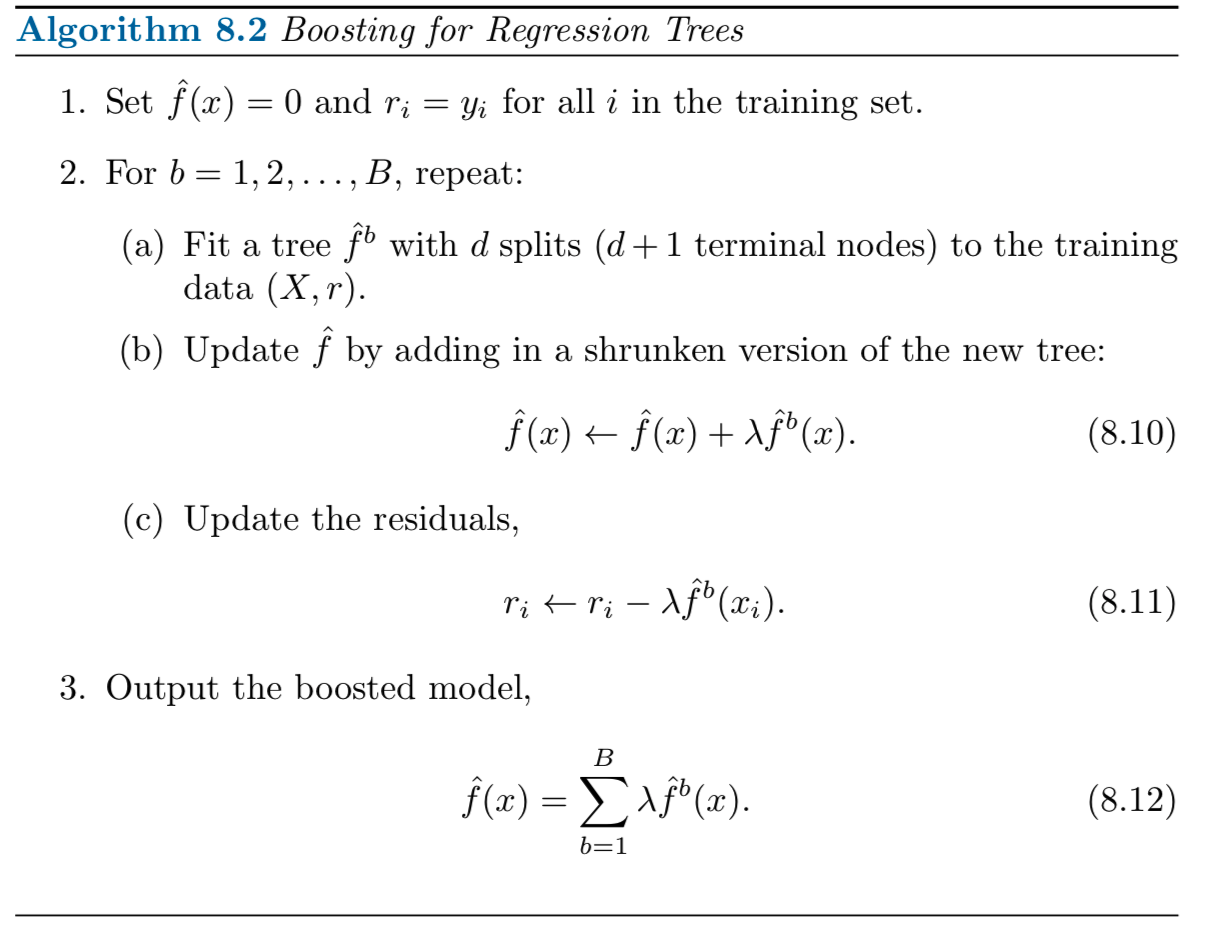
\includegraphics[scale=0.25]{src/ISLR-BOOSTING-ALGO.png}
\end{enumerate}
\textbf{Note sur les exercices:} 
	\begin{enumerate}
	\item	Des questions sur le bagging, foret aléatoires, boosting seraient qualitatives et non quantitatives puisqu'elles nécessitent beaucoup de puissance informatique;
	\end{enumerate}
\end{CHPT_SUMM}

\subsection{Notes sur les vidéos YouTube}

%\begin{YTB_SUMM}[label = TREES-PART1]{\href{https://www.youtube.com/watch?v=7VeUPuFGJHk&list=PLblh5JKOoLUICTaGLRoHQDuF_7q2GfuJF&index=34}{StatQuest: Decision Trees}}
%\begin{itemize}
%	\item	Different types of nodes;
%	\item	Binary splitting;
%	\item	Selecting first sub-node from the Root node;
%		\item[]	First test for root node's variable is to find which predictor best predicts it ;
%	\item	Nodes not perfectly predicting are \textit{impure};
%		\item[]	Gini impurity is the measure for measuring the impurity of a node with the sub-nodes;
%		\item[]	Total Gini impurity is a weighed average of the proportion of people in each sub-node;
%		\item[]	Compare total gini impurities to see which variable predicts best and should be the root node variable
%\end{itemize}
%\end{YTB_SUMM}
%
%\begin{YTB_SUMM}[label = RANDOMFORESTS-BAGGING]{\href{https://www.youtube.com/watch?v=7VeUPuFGJHk&list=PLblh5JKOoLUICTaGLRoHQDuF_7q2GfuJF&index=34}{StatQuest: Decision Trees}}
%\begin{itemize}
%	\item	Bootstrapped dataset: create new samples from an existing training set of samples which are just random combinations of them;
%	\item	Create a bunch of decision trees with a random number of the variables;
%	\item	Repeat this a bunch of times;
%	\item	This is \textbf{Bagging}---\textbf{B}ootstrapping the data and using the \textbf{agg}regrate to make a decision;
%	\item	The \textbf{Out-Of-Bag} dataset is the data that didn't wind up in the data used;
%	\item[]	Typically, around a third of the data doesn't wind up in the bootstrapped data set;
%	\item[]	Josh would've called it \textbf{Out-of-Boot} data set since it's the samples which didn't make it into the bootstrap dataset;
%	\item[]	It is used to test the tree'
%	\item	The proportion of Out-Of-Bag samples which were incorrectly labed is the \textbf{Out-Of-Bag Error}
%\end{itemize}
%\end{YTB_SUMM}

\begin{YTB_SUMM}[label = TREES-REGRESSION]{\href{https://www.youtube.com/watch?v=g9c66TUylZ4&list=PLblh5JKOoLUICTaGLRoHQDuF_7q2GfuJF&index=36}{StatQuest: Regression Trees, Clearly Explained!!!}}
\begin{itemize}
	\item	Alternative to a straight line for predictions;
	\item	Each leaf represents a numerical value;
	\item[]	In constrast, classification trees have a True/False, or a category, in their leaves;
	\item	Average value of group corresponding to the test, for example:
	
	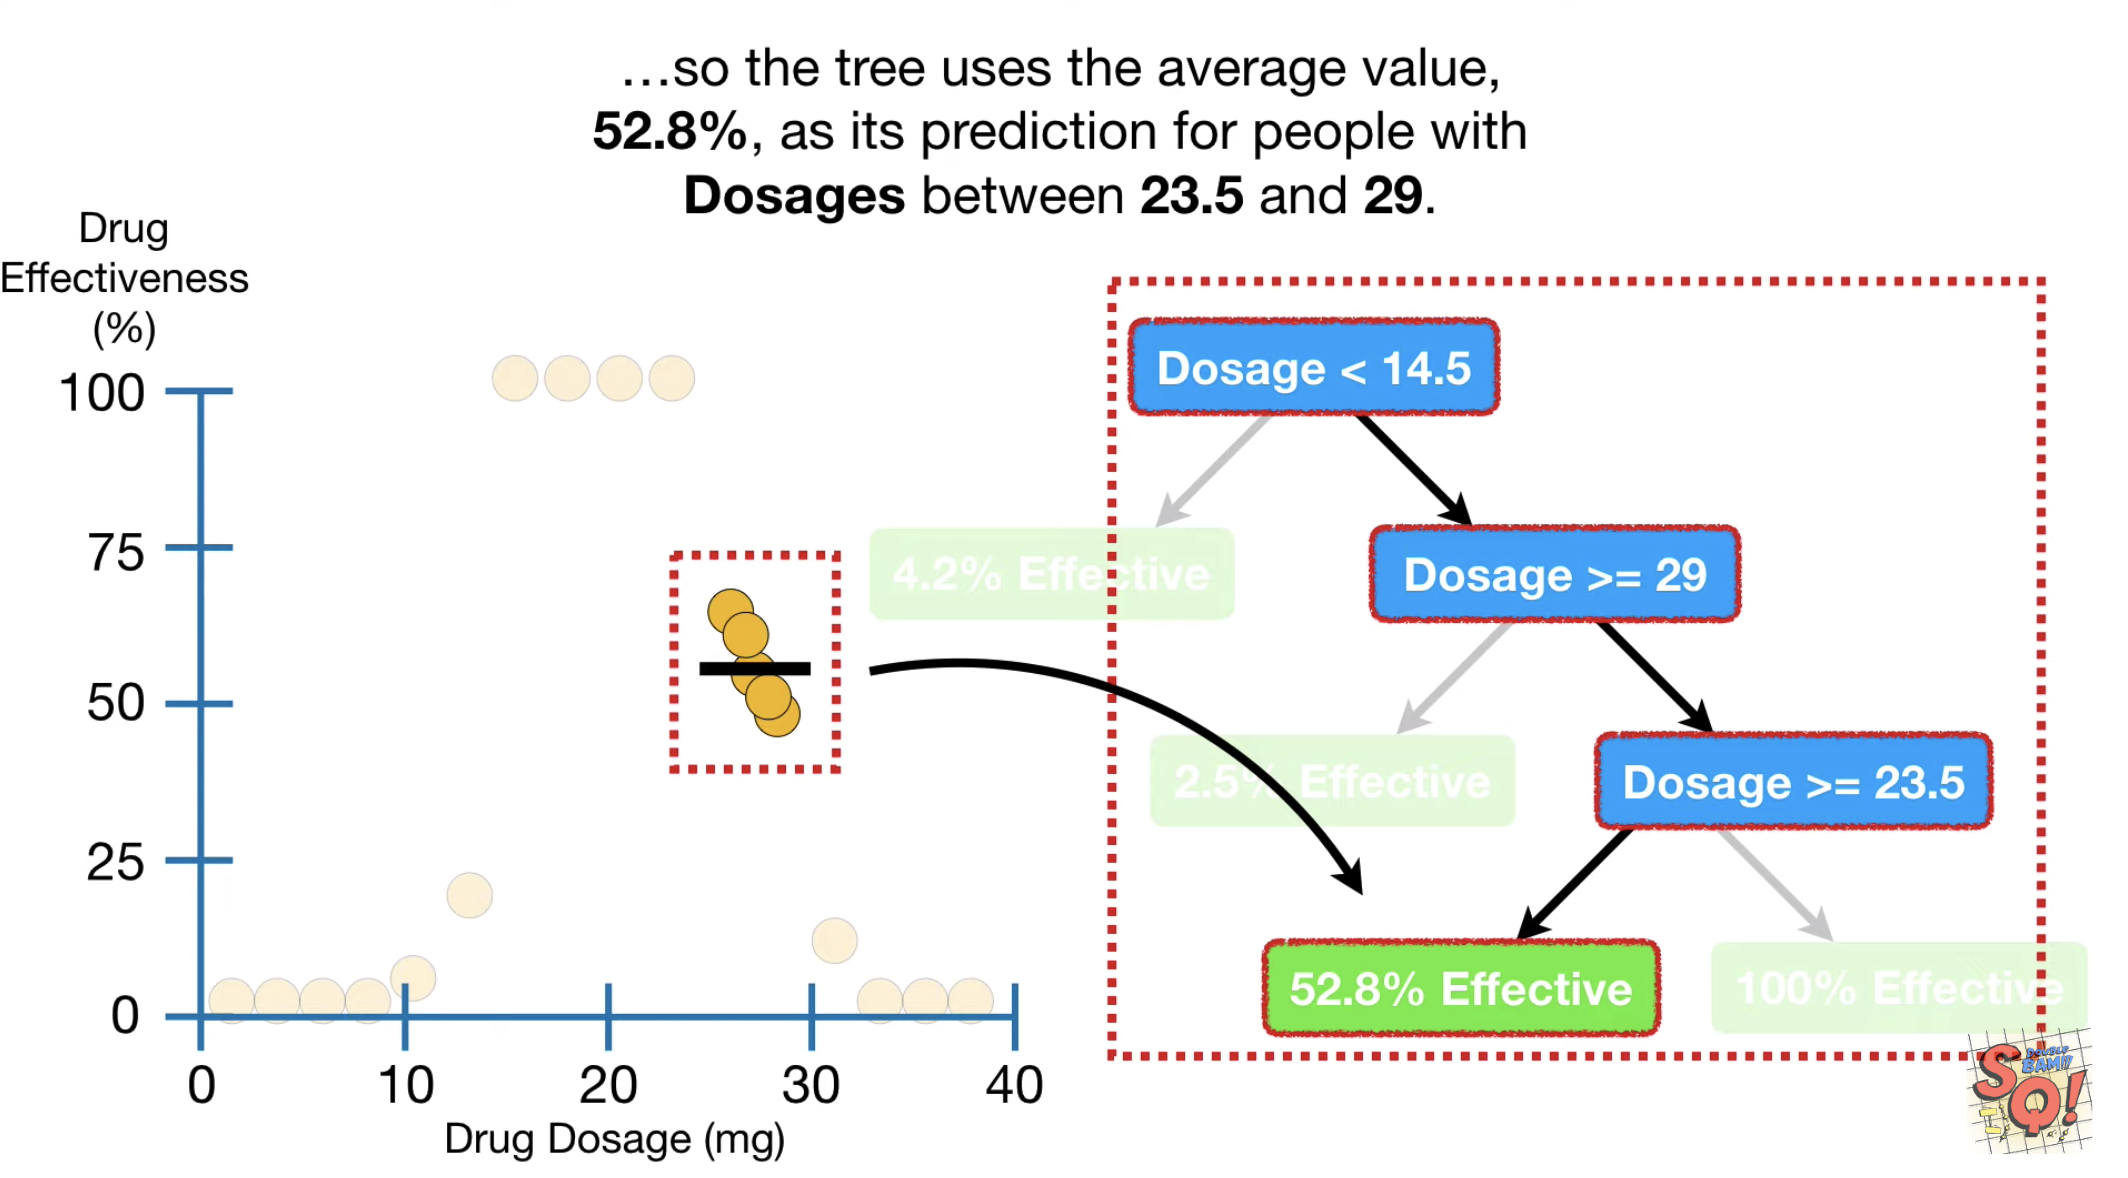
\includegraphics[scale=0.3]{src/SQ-TREES-REGRESSION.png}
	\item	Because of the way the data's formed, with clusters of information, the tree will do a better job reflecting the data than a straight line;
	\item	The graph is just as easy to use to predict with one predictor and only a bit of data but with many predictors and alot of data it becomes much less conveniant;
	\item[]	In contrast, a decision tree will be just as simple with the extra predictors;
	\item	Split data into groups by finding threshold giving the smallest SS(residuals);
	\item	When model fits training data perfectly, probably means overfit and won't perform well with testing data;
	\item[]	It has low bias and a high variance;
	\item	One way to treat is to split only above a certain number of observations;
	\item[]	For example, if there's less than 20 observations don't split the node;
%	
	\item	With several predictors?
	\item[]	Find threshold with lowest SS(residual) for each variable and pick the variable having the lowerst overall SS(residual);
	\item	In brief;
	\item[]	Regression trees are a type of decision trees;
	\item[]	Determine how to divide observations by trying different thresholds and calculating the SS(residuals) at each step;
	\item[]	With multiple, calculate most optimal threshold for each and pick lowest overall;
	\item[]	Split until we have less observations than our required minimum in a group;
\end{itemize}
\end{YTB_SUMM}

\begin{YTB_SUMM}[label = {TREES-PRUNING}]{\href{https://www.youtube.com/watch?v=D0efHEJsfHo&list=PLblh5JKOoLUICTaGLRoHQDuF_7q2GfuJF&index=37}{StatQuest: How to Prune Regression Trees, Clearly Explained!!!}}
\begin{itemize}
	\item	Each leaf corresponds to the average druf effectiveness from a different cluster of observations;
	\item	Residuals are small in some areas and large in others;
	\item[]	The 4 in the middle now look like outliers, meaning we overfit the tree;
	\item[]	One way to prevent overfitting is to remove some of the leaves and replace them with the average of a larger number of observations;
	\item	The main idea of pruning data, is preventing overfitting the training data;
	\item	Theoretically, we could keep \textit{going up} and removing leaves, but how do we decide which tree to use (how many nodes to remove)?
	\item[]	With \textbf{cost complexity pruning};
	\item	Each time we prune the tree, SS(residuals) gets larger;
	\item[]	However, we \textit{want this} as the idea is the prune tree \textit{won't fit} the data as well as the full sized tree;
	\item	So, we have the Tree Score = \textbf{SSR} + $\alpha$\textbf{T};
	\item	$\alpha$ is a tuning parameter found with cross-validation;
	\item	So select tree with smallest tree score;
	\item[]	$\alpha$ \textit{makes a big difference} on decision;
%	
		\begin{enumerate}
		\item	Fit a full-sized tree with all the data (training and testing);
		\item[]	Note $\alpha = 0$ is of course the smallest penalty possible;
		\item	Increase $\alpha$ until pruning leaves leads to a lower score;
		\item[]	We obtain $\alpha = 10 000$;
		\item	Repeat and find different threshold values for $\alpha$;
		\item	Fit trees with oonly the training data for each of the same thresholds;
		\item[]	Select tree having smallest SS(residuals) with the testing data;
		\item	Repeat 10 times with different seperations of training and testing data for 10-fold cross-validation;
		\end{enumerate}
\end{itemize}
\end{YTB_SUMM}

\newpage
\chapter[Cluster Analysis]{Cluster Analysis (10\% à 15\%)}

\subsubsection{Information}

\begin{distributions}[Objective]
Understand key concepts concerning cluster analysis
\end{distributions}

\begin{outcomes}[Learning outcomes]
\begin{enumerate}
	\item	Expliquer les utilités du \og clustering \fg{}.
	\item	Expliquer le \og $K$-means clustering \fg{}.
	\item	Expliquer le \og hierarchical clustering \fg{}.
	\item	Expliquer les méthodes pour décider le nombre de \og clusters \fg{} 
	\item	Comparer le \og hierarchical \fg{} contre le \og $K$-means clustering \fg{}.
\end{enumerate}
\end{outcomes}

\begin{ASM_chapter}[Related lessons ASM]
\begin{enumerate}
  \setcounter{enumi}{17}
	\item	\hyperref[CLUSTERS]{Cluster Analysis}
\end{enumerate}
\end{ASM_chapter}

\begin{YTB_vids}[Vidéos YouTube]
\begin{itemize}
	\item	\href{https://www.youtube.com/watch?v=4b5d3muPQmA&list=PLblh5JKOoLUICTaGLRoHQDuF_7q2GfuJF&index=32}{StatQuest: K-means clustering}
	\item	\href{https://www.youtube.com/watch?v=7xHsRkOdVwo&list=PLblh5JKOoLUICTaGLRoHQDuF_7q2GfuJF&index=31}{StatQuest: Hierarchical Clustering}
\end{itemize}
\end{YTB_vids}

\subsection{Résumés des chapitres}

\begin{CHPT_SUMM}[label = {CLUSTERS}]{\addcontentsline{toc}{subsubsection}{18. Cluster Analysis}18. Cluster Analysis}
\begin{enumerate}
	\item	\textbf{Descriptions}
		\begin{itemize}
		\item	Méthode d'apprentissage non supervisée;
		\item	Classification des observations dans un petit nombre de regroupements (clusters) avec des observations similaires entre eux;
		\item	Exemples d'applications:		
			\begin{itemize}
			\item	Marketing: classification des clients selon leurs achats afin de viser les clients plus probables d'être intéressés à des produits;
			\item	Médecine: regroupement des patients selon des mesures médicales pour déterminer le meilleur traitement;
			\item	Modélisation actuarielle: classification des polices en catégories (cells) pour la tarification;
			\end{itemize}
		\end{itemize}
%%%
	\item	\textbf{$K$-means} clustering
%	
	\item[]	\textbf{Description}
		\begin{itemize}
		\item	On pose $p$ variables vecteurs $\bm{X}_{j}$ et $n$ observations telles que $\bm{X}_{j} = \{x_{1j}, x_{2j}, \dots, x_{nj}\}$;
		\item[]	\textbf{Note}: Une observation correspond alors au vecteur des $i^{\text{e}}$ termes de chacune des $p$ variables $\{x_{ip}, x_{ip}, \dots, x_{ip}\}$;
		\item	On pose un nombre, $K$, de clusters $C_{1}, \dots, C_{K}$ avant la classification;
		\item	Toutes les observations sont assignées à un groupe, la classification est dite \textit{exhaustive};
		\item	Aucune observation n'est assignée à plus d'un cluster, la classification est dite \textit{mutuellement exclusive};
		\end{itemize}
%
	\item[]	Optimisation théorique
		\begin{itemize}
		\item	On cherche à minimiser la somme des $K$ dissemblances totales inter-cluster $W(C_{k})$: 
		\begin{align*}
			\min	\sum_{k = 1}^{K} W(C_{k})
		\end{align*}
		\item	Souvent, la mesure de dissemblance $W(C_{k})$ est définie avec la distance euclidienne des points au centroïde:
			\begin{align*}
			W(C_{k})	
			&=	\frac{1}{|C_{k}|} \sum_{i, i' \in C_{k}} \sum_{j = 1}^{p} (x_{ij} - x_{i'j})^{2}
			\end{align*}
		\item[]	$|C_{k}|$ peut être vu comme le $n$ habituel, c'est le nombre de points dans le cluster;
		\item	Le problème avec cette méthode est qu'il serait \textit{irréaliste de calculer toutes les possibilités de classification} des points en $K$ clusters afin de trouver celui avec la distance minimale;
		\item	Cependant, on utilise un algorithme qui utilise le centroïde pour trouver le minimum local;
		\end{itemize}
%		
	\item[]	\textbf{Classification}
		\begin{itemize}
		\item	Le $K$-means clustering est en fait un \textit{cas spécial} du \textit{$K$-clusters} clustering car on utilise les \textbf{centroïdes des clusters} pour la classification;
		\item	La méthode \textit{centroïde} consiste à classifier les observations en minimisant les dissemblances entre les points des clusters;
		\item	Le \textit{centroïde} d'un cluster est le point ayant comme coordonnées la moyenne des coordonnées des points dans le cluster;
		\item	Formellement, ceci est:
			\begin{align*}
				\bar{x}_{kj}	&=	\frac{1}{|C_{k}|} \sum_{i \in C_{k}} x_{ij}
			\end{align*}
			Mais il est bien plus simple de visualiser la signifiance d'un centroïde que de tenter de déchiffrer cette formule;
		\item	Avec ceci, on peut reformuler $W(C_{k})$ avec l'identité suivante:
			\begin{align*}
			W(C_{k})	
			&=	\frac{1}{|C_{k}|} \sum_{i, i' \in C_{k}} \sum_{j = 1}^{p} (x_{ij} - x_{i'j})^{2}	\\
			&\Leftrightarrow	2 \sum_{i \in C_{k}} \sum_{j = 1}^{p} (x_{ij} - \bar{x}_{kj})^{2}	\\
			\end{align*}
		\item	L'algorithme est:
			\begin{enumerate}[label = \roman*.]
			\item	Arbitrairement, classez les observations en $K$ clusters;
			\item	Pour chacun des clusters, calculer le centroïde;
			\item	Créer de nouveaux clusters en associant chaque point au centroïde le plus près;
			\item	Répéter la 2e et 3e étape jusqu'à ce que les points restent fixes;
			\end{enumerate}
		\end{itemize}
	\item[]	\textbf{Problèmes}
		\begin{itemize}
		\item	L'algorithme doit être \textit{répété plusieurs fois} pour avoir une bonne chance d'arriver à la bonne réponse;
		\item	Choisir $K$ est compliqué et arbitraire;
		\end{itemize}
%%%	
	\item	\textbf{Hierarchical} clustering
	\item[]	\textbf{Description}
		\begin{itemize}
		\item	Le \textit{hierarchical clustering} est un alternatif qui n'exige pas la spécification du nombre de clusters a priori;
		\item	C'est plutôt comme un \textit{arbre} de gros clusters composés de plus petits clusters composés de ... ;
		\item	Le \textbf{Bottom-up} clustering est nommé après le dendrogramme montrant les fusions à partir d'en bas montant jusqu'à un cluster général en haut;
		\item[]	Ce faisant, il est aussi nommé \textit{agglomerative clustering};
		\end{itemize}
	\item[]	\textbf{Liaison} \textit{(linkage)}: Sert à définir, et mesurer, la dissemblance entre groupes d'observations (clusters);
%		\item	À terme d'exemple, imaginons que nous avons les points $\{0, 1, 2, 5, 7, 10\}$ en groupes arbitraires $\{0, 5\}$, $\{7\}$ et $\{1, 3, 10\}$;
		\begin{enumerate}
		\item	\textbf{Complete} linkage: On mesure la distance maximale entre les deux points les plus éloignés de clusters et on prends la minimale de ceux ci;
%			\item[]	Par exemple, les distances de l'exemple sont $7 - 0 = 7$, $7 - 1 = 6$ et $10 - 0 = 10$;
%			\item[]	Ce faisant, les nouveaux groupes seraient $\{0, 5\}$ et $\{1, 3, 7, 10\}$;
		\item	\textbf{Single} linkage: Au lieu de mesurer la distance maximale, on mesure la distance minimal puis on regroupe;
%			\item[]	Par exemple, les distances de l'exemple sont $7 - 5 = 2$, $10 - 7 = 3$ et $5 - 3 = 2$;
%			\item[]	Ceci est un exemple d'où l'algorithme est pris dans un minimum local;
%			\item[]	Il faudrait recommencer l'algorithme avec de différents groupes
		\item	\textbf{Average} linkage: On prends la moyenne des distances entres tous les points des deux clusters et on fusionne ceux ayant la plus faible distance moyenne;
		\item	\textbf{Centroid} linkage: On assigne un point \textit{centroïde} à chaque cluster ayant comme coordonnées la moyenne des coordonnées des points du clusters et on minimise la distance entre centroïdes;
		\end{enumerate}
	\item[]	\textbf{Mesures de dissemblance}
		\begin{itemize}
		\item	Malgré que la distance euclidienne est souvent utilisée, différentes mesures sont possibles;
		\item	StatQuest explique le \textit{Manhattan Distance} et le livre la mesure basée sur la corrélation;
		\item	Ce qu'on doit en retirer est que différentes mesures ont différents impacts et donc qu'il faut considérer les applications pour décider quelle mesure choisir;
		\item	Pour exemple, on cherche à regrouper des clients d'Amazon par leurs historiques d'achats;
		\item	La distance euclidienne va regrouper les clients ayant acheté peu d'items --- des clients allant moins fréquemment au site; 
		\item	On voit donc que ceci n'est pas nécessairement ce que l'on veut;
		\item	En contraste, une mesure de corrélation va regrouper des clients avec des historiques d'achat semblables;
		\item	Il n'y a pas de solution simple, il faut songer au contexte et au but du clustering pour trancher;
		\end{itemize}
	\item[]	\textbf{Scaling}
		\begin{itemize}
		\item	Comme pour le $K$-means clustering, on doit songer à s'il est nécessaire de ramener les variables sur la même échelle;
		\item	Clairement, \textit{une} télévision est moins que \textit{dix} bas, mais est-ce qu'il est approprié de faire cette comparaison?
		\item[]	Sans scaling, les bas auront un impact beaucoup plus significatif;
		\item	Lorsque nous comparons des kilomètres contre des centimètres, la réponse est simple, mais en unités ça \textit{dépends du contexte};
		\item	Voici un bel exemple du livre:
		\end{itemize}
		
	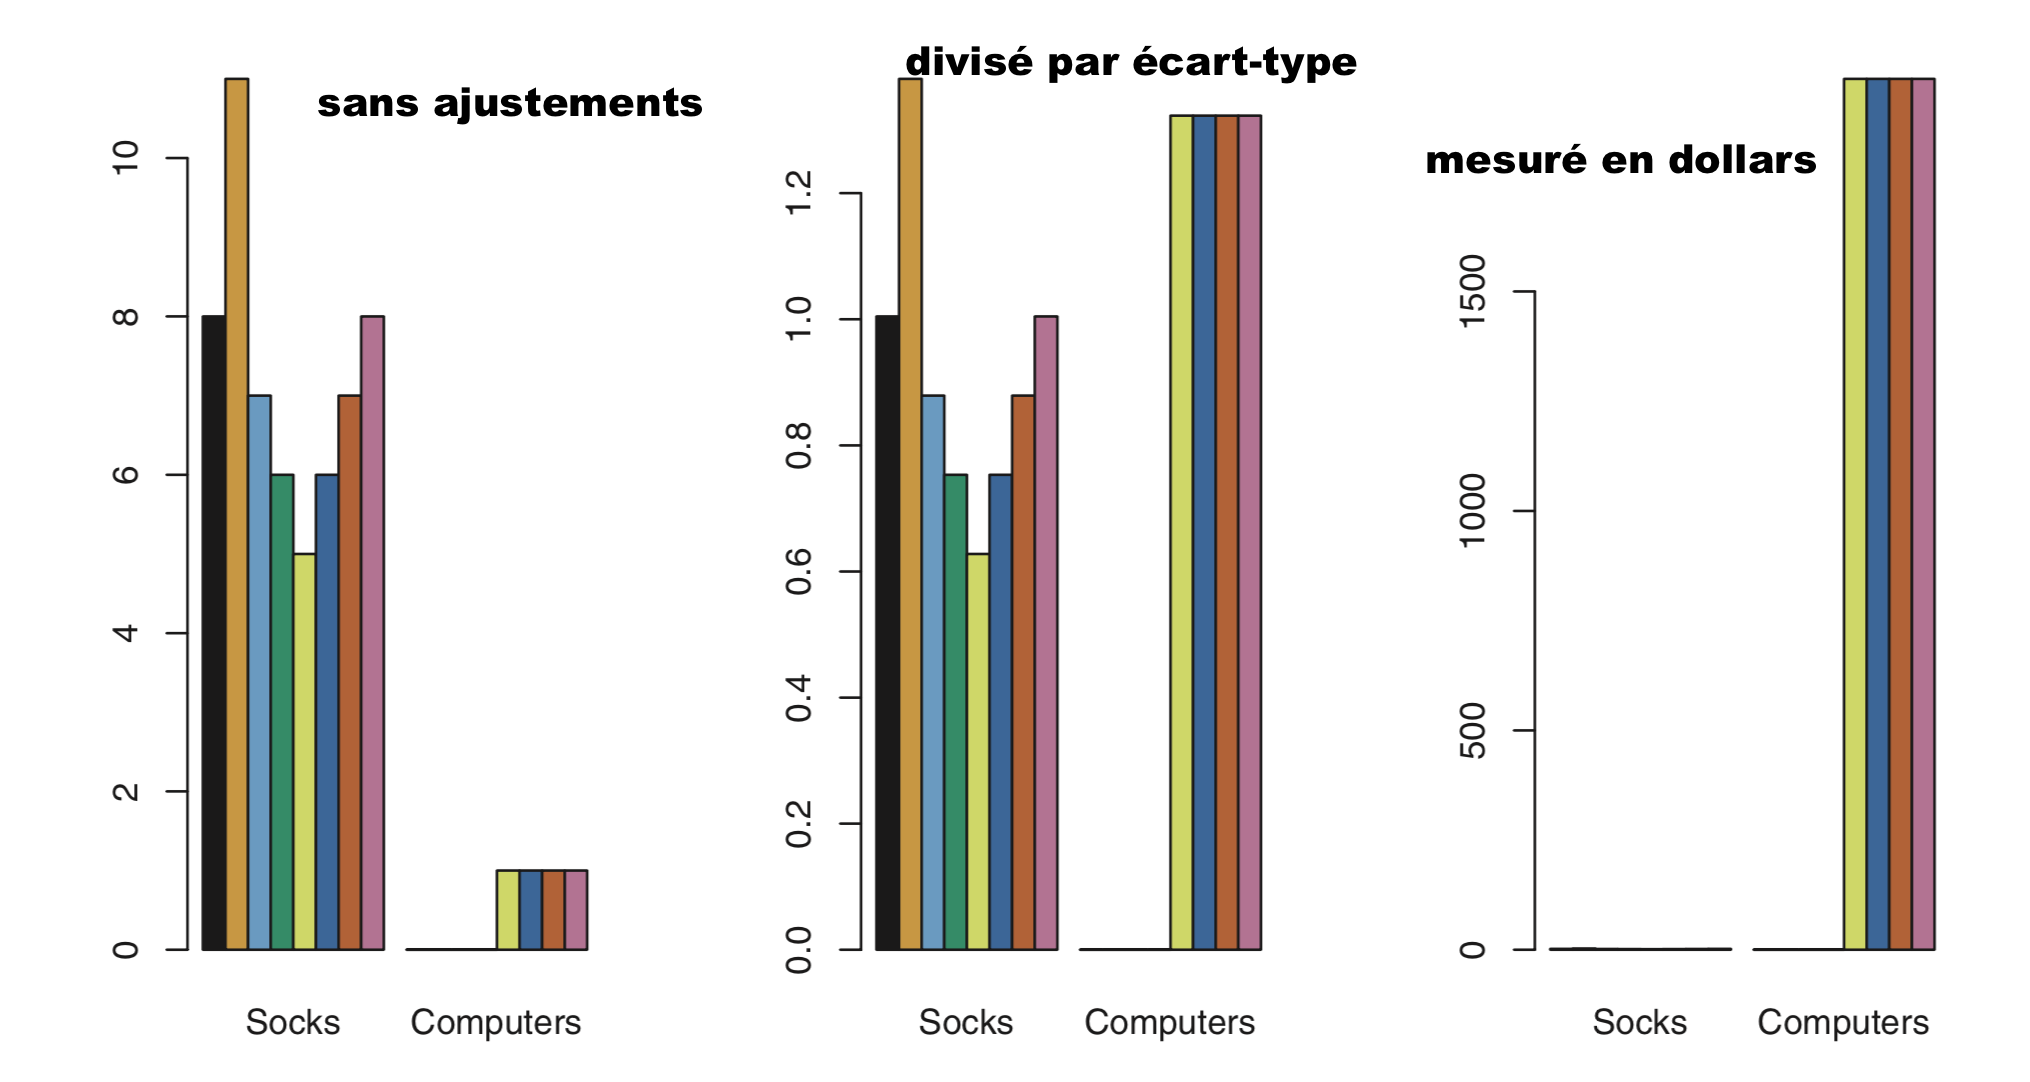
\includegraphics[scale=0.3]{src/ISLR-HIERARCH-SCALE.png}
%%%	
	\item	\textbf{Problèmes et considérations} avec le clustering
		\begin{itemize}
		\item	Le hierarchical clustering suppose qu'une hiérarchie existe;
		\item[]	Pour exemple, si les variables sont le sexe et la race, alors le $K$-means clustering sera mieux ajusté;
		\item	Il y a également les problèmes d'échelle et de mesure de dissemblance;
		\item	Il est difficile de valider les clusters, comment savoir si ce sont des vrais regroupements ou si l'on \textit{cluster the noise}?
		\item	Nous forçons \textit{tous} les observations à appartenir à un groupe, ce faisant les outliers peuvent déformer les clusters;
		\item	Le clustering n'est pas une méthode robuste;
		\item[]	On peut retirer un point, recommencer la procédure et arriver à des clusters entièrement différents;
		\end{itemize}
%		
	\item[]	Il y a également plusieurs \textbf{décisions} à prendre ayant toutes un impact sur le résultat:
		\begin{enumerate}[label = \roman*.]
		\item	Quelle méthode de clustering est plus appropriée?
		\item	Est-ce que les variables devraient être mises à l'échelle?
		\item	Combien de clusters ($K$-means)?
		\item	Quelle mesure de dissemblance devrait être utilisée (hierarchical)?
		\item	Quelle méthode de liaison (hierarchical)?
		\item	À quelle hauteur partitionner le dendrogramme (hierarchical)?
		\end{enumerate}
	\item[]	En pratique, on veut donc essayer plusieurs résultats et analyser avant de faire de décisions;
\end{enumerate}
\textbf{Note sur les exercices:} 
\begin{enumerate}
	\item	En gros ce n'est pas compliqué, faut le pratiquer un peu pour être à l'aise à le faire;
	\item	Pour les questions qualitatives faut vraiment prendre le temps de bien lire et bien saisir---vidéo de StatQuest essentiel;
	\item	Examen aura des choix multiples où il faut comparer les méthodes (voir 18.12), interpréter le clustering (18.1), etc. (18.9);
	\item	Faire une itération d'un $K$-means assurément (2, 3, 10, 11);
	\item	Faire une itération / le hierarchical clustering assurément (5, 6, 7, 8);
\end{enumerate}
\end{CHPT_SUMM}

\begin{FORMULA_SUMM}{Formules cool}
La \textbf{distance Minkowski}, entre deux variables $X$ et $Y$, est la généralisation de la distance euclidienne ($p = 2$) et Manhattan ($p = 1$):
\begin{align*}
	\left( \sum_{i = 1}^{n} | X_{i} - Y_{i} |^{p} \right)^{1/p}
\end{align*}
\end{FORMULA_SUMM}

\subsection{Notes sur les vidéos YouTube}

\begin{YTB_SUMM}{\href{https://www.youtube.com/watch?v=7xHsRkOdVwo&list=PLblh5JKOoLUICTaGLRoHQDuF_7q2GfuJF&index=31}{StatQuest: Hierarchical Clustering}}
\begin{itemize}
	\item	We have the following example:
	
	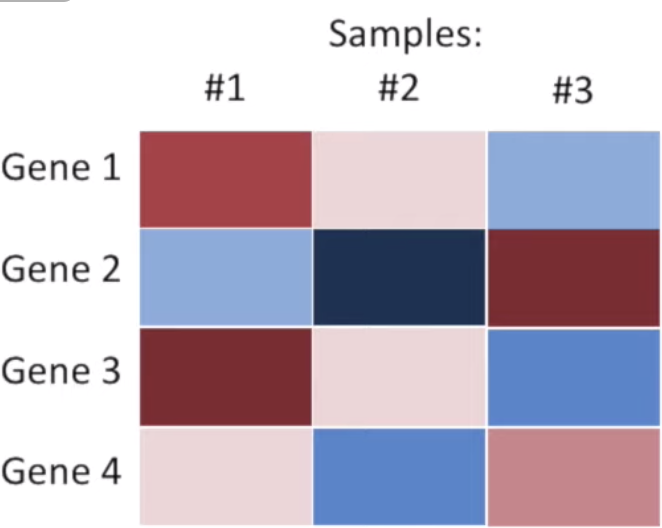
\includegraphics[scale=0.4]{src/SQ-HIERARCH-heatmap.png}
	\item[]	Red means highly expressed while blue is the opposite
	\item	Steps:
		\begin{enumerate}
		\item	Figure out which gene is most similar to gene \# 1;
		\item[]	We see \# 1 and \# 3 are very similar;
		\item	Figure out which genre is most similar to gene \# 2;
		\item[]	We see \# 2 and \# 4 are very similar;
		\item[]	We then repeat this for genes \# 3 and \# 4;
		\item	Of the possible combinations we figure out which 2 genes are the most similar and merge them into a cluster;
		\item[]	Thus, we see that genes \# 3 and \# 4 are most similar than any other combination of genes and merge them:
		
		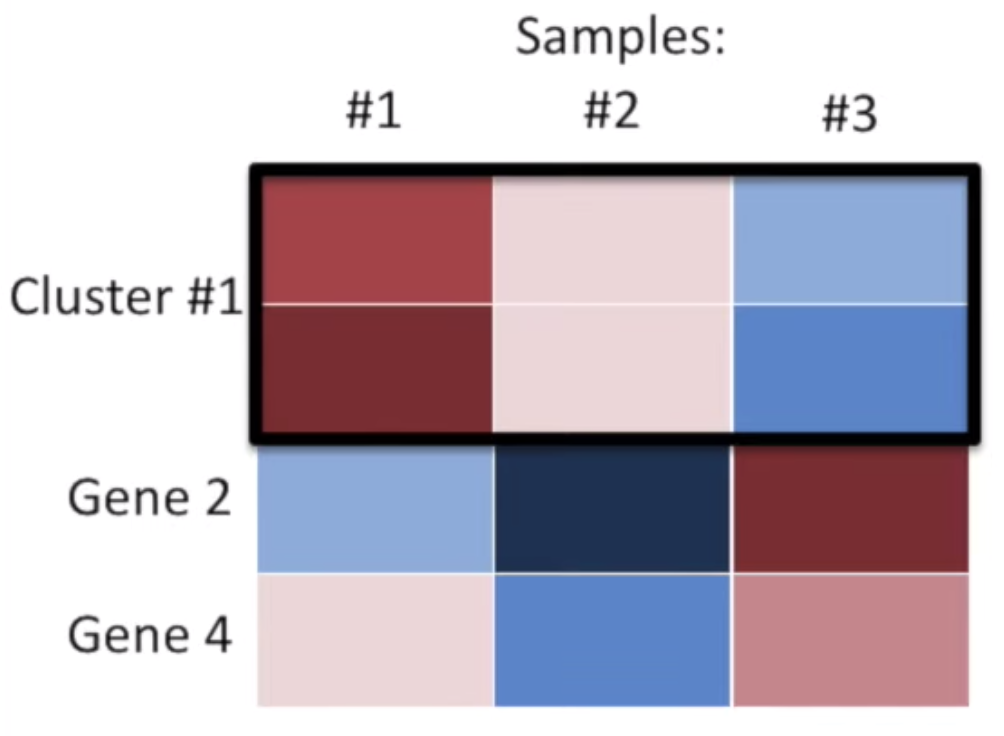
\includegraphics[scale=0.4]{src/SQ-HIERARCH-heatmap-cluster.png}
		\item	Repeat from step \# 1 treating the cluster as a single gene;
		\item[]	We see cluster number 1 is most similar to gene \# 4;
		\item	We then see gene \# 2 is most similar to gene \# 4 
		\item[]	We repeat for gene \# 4 as well;
		\item	We then merge genes \# 2 and \# 4 into one cluster as they're the most similar:
		
		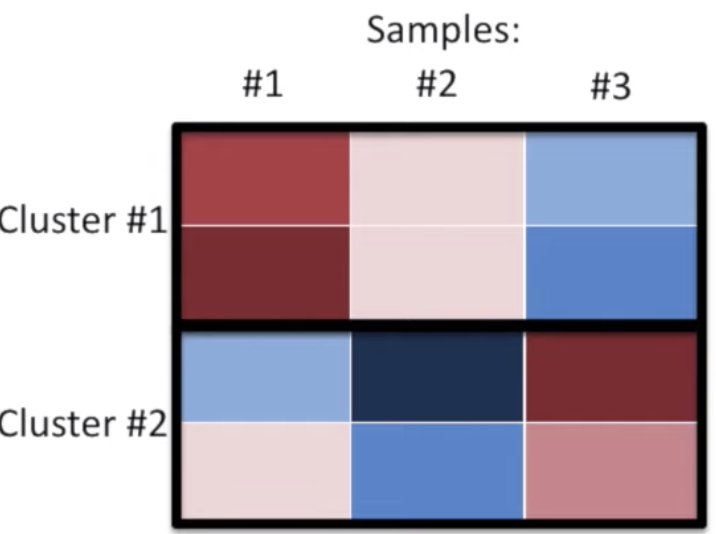
\includegraphics[scale=0.4]{src/SQ-HIERARCH-heatmap-cluster-2.png}
		\item	We go back to the first step, but since there's only 2 clusters left we merge them;
		\end{enumerate}
	\item	After clustering, we have the dendrogram indicating both order and similarity:
	
	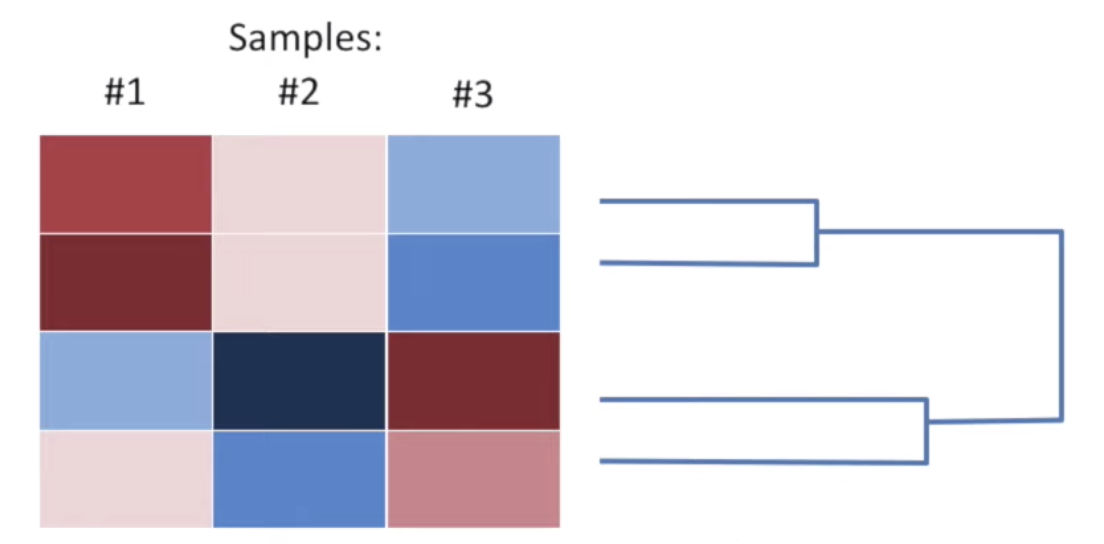
\includegraphics[scale=0.4]{src/SQ-HIERARCH-heatmap-cluster-dendrogram.png}
	\item[]	Cluster \# 1 was formed first and was the most similar, therefore it has the shortest branch;
	\item[]	Cluster \# 2 was formed second and was the second most similarity thus it has the second shortest branch;
	\item[]	Cluster \# 3 was formed last and and has the longest branch;
	\item	How do we define \textit{most similar}?
	\item[]	Often the \textit{Euclidian distance} which is just the distance between 2 points with the pythagorean theorem;
	\item[]	Alternatives to this include the \textit{Manhattan distance} which is the absolute value of the differences;
	\item[]	Unfortunately \textit{different distance metrics} \textit{have an impact} but the choice is arbitrary;
	\item	How do we \textit{merge} and compare clusters ?
	\item[]	Often the average is used (the \textit{centroid} method), but there's others;
	\item[]	For example, if we wanted to assign a point to 2 predefined groups :
	
	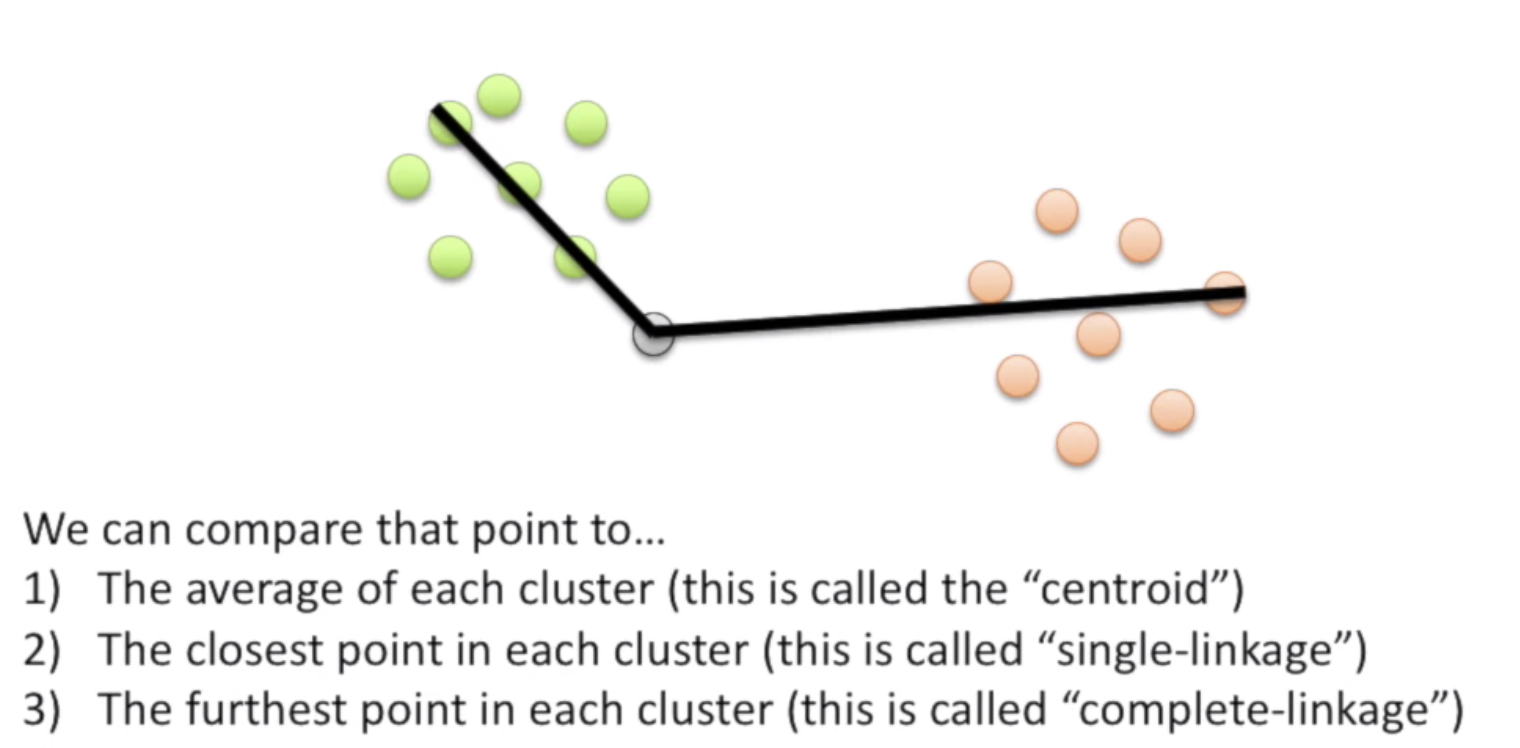
\includegraphics[scale=0.4]{src/SQ-HIERARCH-METRICS.png}
	\item[]	Like for the similarity, different measures have different impacts;
	\item[]	For example:
	
	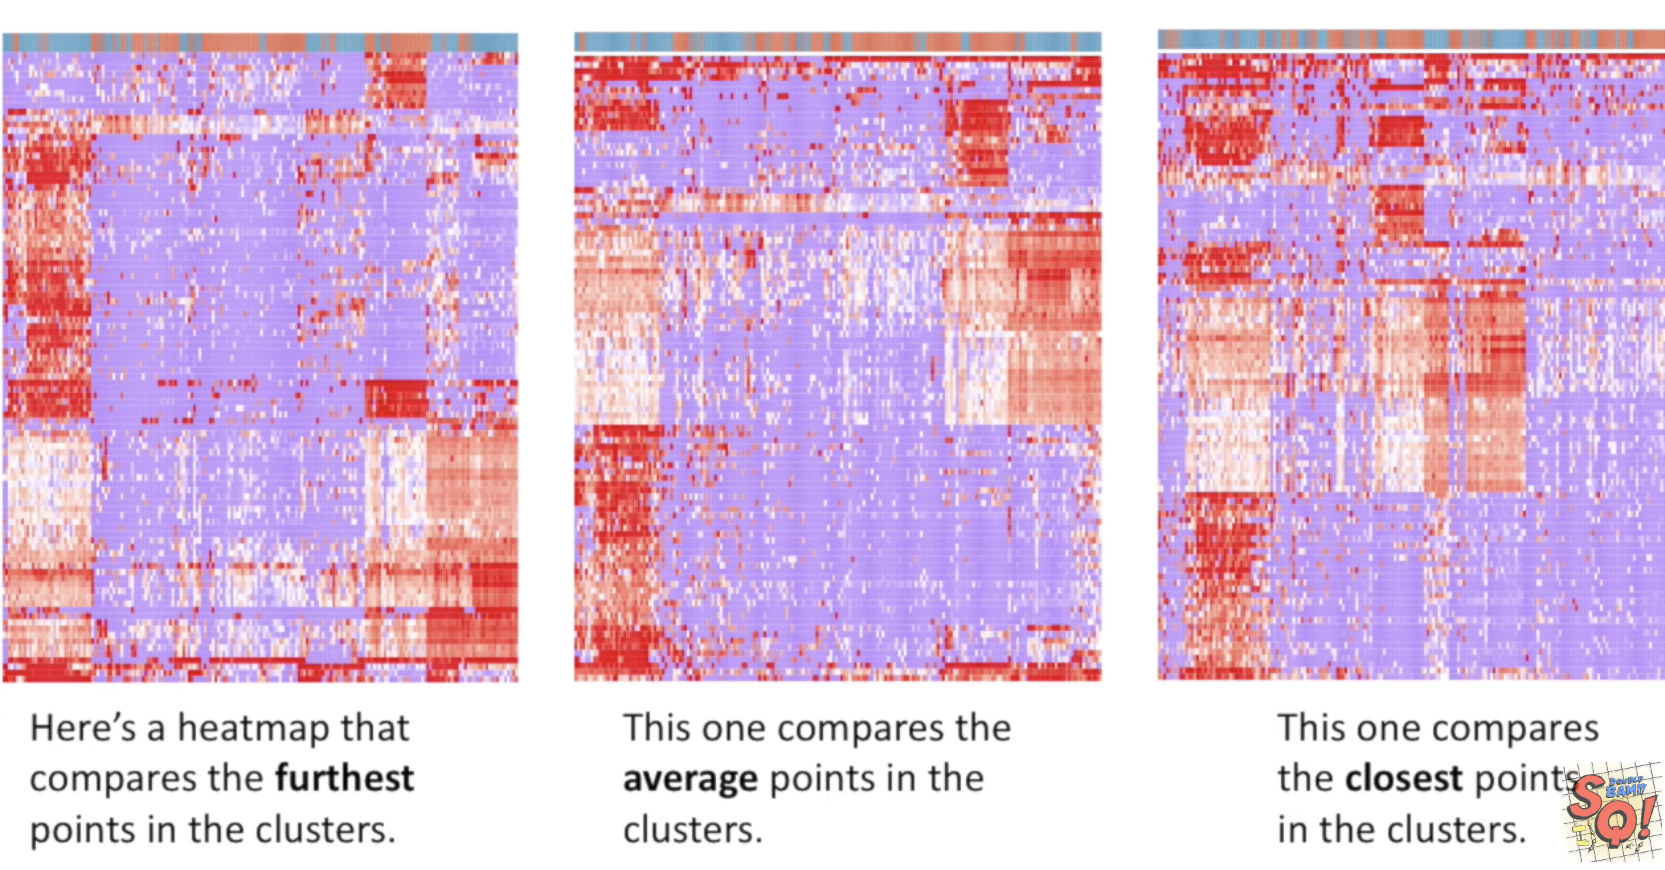
\includegraphics[scale=0.4]{src/SQ-HIERARCH-METRICS-IMPACT.png}
	\item	En bref: 
		\begin{enumerate}
		\item	Clusters are formed based on some notion of \textit{similarity};
		\item	Once we have a sub-cluster, we must decide how we \textit{compare} it to other sub-clusters/columns/rows/etc.
		\item	The \textit{height of the branches} in dendrograms show you \textit{what is most similar};
		\end{enumerate}
\end{itemize}
\end{YTB_SUMM}

\end{document}
